% Authoritative English source. Edit chapter files in en/, then run build.py.
\documentclass[11pt,a4paper,oneside]{report}
\newcommand{\EditionShort}{EN}
% Shared typography for both authoritative language editions.
\usepackage[a4paper,left=20mm,right=18mm,top=22mm,bottom=22mm,headheight=16pt,headsep=7mm]{geometry}
\usepackage{fontspec}
\usepackage{kotex}
\setmainfont{TeX Gyre Pagella}
\setsansfont{TeX Gyre Heros}
\setmonofont{DejaVu Sans Mono}[Scale=0.83]
\setmainhangulfont{Noto Serif CJK KR}
\setsanshangulfont{Noto Sans CJK KR}
\setmonohangulfont{Noto Sans CJK KR}
\setmainhanjafont{Noto Serif CJK KR}
\usepackage{amsmath,amssymb}
\usepackage{fix-cm}
\usepackage{xcolor}
\definecolor{ocrtNavy}{HTML}{18384D}
\definecolor{ocrtTeal}{HTML}{167C89}
\definecolor{ocrtLine}{HTML}{C8D5DC}
\definecolor{ocrtGray}{HTML}{52616B}
\usepackage{array,longtable,booktabs}
% LaTeX 2025 mark extraction can report infinite shrink from longtable's
% trailing \vss. Keep its stretch and replace infinite with finite shrink.
% No-op for package versions that do not contain these two occurrences.
\usepackage{etoolbox}
\usepackage{tikz}
\usetikzlibrary{arrows.meta,calc,angles,quotes,positioning,decorations.pathreplacing}
\usepackage{pgfplots}
\pgfplotsset{compat=1.18}
\usepackage{caption}
\usepackage{float}
\captionsetup{font=small,labelfont=bf,labelsep=period,justification=raggedright,singlelinecheck=false}
\usepackage[section]{placeins}
\newcommand{\FigLang}[2]{\ifdefstring{\EditionShort}{KO}{#1}{#2}}
\makeatletter
\patchcmd{\LT@output}{\vss}{\vskip 0pt plus 1fil minus \textheight\relax}{}{}
\patchcmd{\LT@output}{\vss}{\vskip 0pt plus 1fil minus \textheight\relax}{}{}
\makeatother
\usepackage{enumitem}
\setlist{nosep,leftmargin=1.5em,topsep=4pt,parsep=2pt,itemsep=2pt}
\usepackage{fvextra}
\usepackage{titlesec}
\usepackage{needspace}
\titleformat{\chapter}[display]{\sffamily\bfseries\raggedright\color{ocrtNavy}}{\fontsize{11}{14}\selectfont\chaptertitlename\ \thechapter}{5pt}{\fontsize{23}{28}\selectfont}
\titlespacing*{\chapter}{0pt}{0pt}{15pt}
\titleformat{\section}{\sffamily\bfseries\large\color{ocrtNavy}}{\thesection}{0.7em}{}
\titleformat{\subsection}{\sffamily\bfseries\normalsize\color{ocrtNavy}}{\thesubsection}{0.7em}{}
\titleformat{\subsubsection}{\sffamily\bfseries\normalsize\color{ocrtNavy}}{}{0em}{}
\titlespacing*{\section}{0pt}{14pt}{6pt}
\titlespacing*{\subsection}{0pt}{10pt}{4pt}
\usepackage{fancyhdr}
\pagestyle{fancy}
\fancyhf{}
\fancyhead[L]{\scriptsize\sffamily\color{ocrtGray}\nouppercase{\leftmark}}
\fancyhead[R]{\scriptsize\sffamily\color{ocrtGray}OCRT | \EditionShort}
\fancyfoot[C]{\small\sffamily\thepage}
\renewcommand{\headrulewidth}{0.3pt}
\fancypagestyle{plain}{\fancyhf{}\fancyfoot[C]{\small\sffamily\thepage}\renewcommand{\headrulewidth}{0pt}}
\usepackage{xurl}
\usepackage[unicode,colorlinks=true,linkcolor=ocrtTeal,urlcolor=ocrtTeal,bookmarksopen=false,pdfencoding=auto]{hyperref}
\usepackage{bookmark}
\setcounter{tocdepth}{1}
\setcounter{secnumdepth}{2}
\setlength{\parindent}{0pt}
\setlength{\parskip}{5pt}
\setlength{\emergencystretch}{3em}
\setlength{\LTpre}{6pt}
\setlength{\LTpost}{8pt}
\setlength{\tabcolsep}{4pt}
\renewcommand{\arraystretch}{1.16}
\raggedbottom
\widowpenalty=10000
\clubpenalty=10000
\newcommand{\TableFont}{\fontsize{8.5}{11.8}\selectfont}
\newcommand{\CodeFont}{\fontsize{8}{10.4}\selectfont}
\newenvironment{ManualCode}{\VerbatimEnvironment\begin{Verbatim}[fontsize=\CodeFont,breaklines=true,breakanywhere=true,breaksymbolleft={},breaksymbolright={},frame=single,rulecolor=\color{ocrtLine},framesep=2.5mm]}{\end{Verbatim}}
\newcommand{\ManualTitlePage}[4]{%
  \begin{titlepage}\thispagestyle{empty}
  {\sffamily\small\color{ocrtTeal}OCRT / USER DOCUMENTATION\par}
  \vspace{23mm}
  {\sffamily\bfseries\fontsize{46}{51}\selectfont\color{ocrtNavy}OCRT\par}
  \vspace{5mm}
  {\sffamily\bfseries\fontsize{27}{34}\selectfont\color{ocrtNavy}#1\par}
  \vspace{6mm}
  {\sffamily\large\color{ocrtGray}Ocean Colour vector Radiative Transfer\par}
  \vspace{9mm}\color{ocrtTeal}\hrule height 1.2pt\color{black}
  \vspace{8mm}{\large #2\par}
  \ifstrempty{#3}{}{\vspace{7mm}{#3\par}}
  \vfill
  {\sffamily\small\color{ocrtGray}C reference release v1.11.1\par}
  \vspace{2mm}{\sffamily\small\color{ocrtGray}2026-09-12\par}
  \ifstrempty{#4}{}{\vspace{5mm}{\small #4\par}}
  \end{titlepage}}

\hypersetup{pdftitle={OCRT User Manual},pdfsubject={Installation, geometry, complete options, LUTs, simulations and file formats},pdfauthor={OCRT project},pdflang={en}}
\begin{document}
\ManualTitlePage{User Manual}{English edition}{}{}
\pagenumbering{roman}
\chapter*{About this manual}
\addcontentsline{toc}{chapter}{About this manual}
OCRT is a radiative transfer code for ocean-colour atmospheric correction and coupled atmosphere--ocean simulations. The main chapters explain OCRT concepts, installation, options, input formats and output interpretation. The opening Quick start walks through a first calculation. Detailed applications, LUT generation, simulation data generation, Python usage and supporting code are covered in the appendices.

The documentation baseline is C reference release v1.11.1, reviewed on 2026-09-11 at source commit:

\texttt{54861c68e35ec5aaa3938fad53e93dc2dfa7eb1d}

The executable version string alone does not identify the current source revision. Python support is documented separately from C.

\textbf{In OCRT, RAA=180 degrees is the direct-sunglint branch.} Read Chapter~\ref{chap:01_concepts_geometry} before converting satellite azimuths or comparing signed Stokes U. For an atmospheric-correction Rayleigh LUT, decide first whether gas absorption, aerosol and direct sunglint are included.

This manual describes the current implementation. Outdated help text, options whose effective behaviour differs from older descriptions, unsupported combinations and untested conditions are identified in the relevant chapters. Successful example runs do not establish scientific accuracy for an entire production grid.

The Korean and English editions use the same chapter structure and option names. LaTeX files in this directory are the source for future revisions; the earlier Markdown files are retained as an initial draft record. Consult the repository \href{https://github.com/brtnt/OCRT/blob/main/LICENSE}{LICENSE} for use and citation conditions.
\tableofcontents
\clearpage
% Authoritative LaTeX quick start. Keep commands aligned with the Korean edition.
\chapter*{Quick start}
\addcontentsline{toc}{chapter}{Quick start}
\label{chap:quick_start}
\markboth{Quick start}{}
\begingroup
\setlength{\parskip}{3pt}
\textbf{Goal: calculate one viewing direction with the C executable, then create a 12-row Rayleigh LUT.}
These examples use no aerosols or underwater particles, so you can start without downloading the large Mie datasets. Choose the preparation commands for your operating system, then continue in the same terminal. If already built, change to the execution directory and start at Step 2. See \hyperref[chap:02_installation]{Chapter~\ref*{chap:02_installation}} for detailed installation instructions.

\section*{1. Prepare to run}
\textbf{Linux / Ubuntu WSL:} GCC 11 or later, Make, and Git are required. If these tools are missing on Ubuntu, first run \texttt{sudo apt-get update} and \texttt{sudo apt-get install build-essential git}. The build below targets x86-64 AVX2 CPUs. For older x86-64 CPUs, replace \texttt{-march=x86-64-v3} with \texttt{-march=x86-64}. Skip \texttt{git clone} if you have already cloned the repository.

\begin{ManualCode}
git clone https://github.com/brtnt/OCRT.git
cd OCRT/code/OCRT_C
BUILD_FLAGS='-std=c11 -O3 -march=x86-64-v3 -ffp-contract=fast'
BUILD_FLAGS+=' -fassociative-math -fno-signed-zeros -fno-trapping-math'
BUILD_FLAGS+=' -DOCRT_FAST_KERNELS -fopenmp -Isrc'
make CFLAGS="$BUILD_FLAGS"
./build/ocrt --version
export OMP_NUM_THREADS=1
GAS_OFF=(--gas-column-h2o 0 --gas-column-o3 0 --gas-column-no2 0
         --gas-column-o2 0 --gas-column-co2 0 --gas-column-ch4 0)
mkdir -p ../../task/quick_start
\end{ManualCode}

\textbf{Windows PowerShell:} Assumes Git and MSYS2 UCRT64 GCC are installed. If GCC is missing, first run \texttt{pacman -S mingw-w64-ucrt-x86\_64-gcc} in the UCRT64 terminal. The PATH below assumes the default MSYS2 installation location. The execution checks for this manual were performed on Linux/WSL.

\begin{ManualCode}
git clone https://github.com/brtnt/OCRT.git
Set-Location OCRT\code\OCRT_C
$env:Path = 'C:\msys64\ucrt64\bin;' + $env:Path
.\build_win.bat
.\build\ocrt_x86-64-v3.exe --version
$env:OMP_NUM_THREADS = '1'
$gasOff = @('--gas-column-h2o','0','--gas-column-o3','0',
  '--gas-column-no2','0','--gas-column-o2','0',
  '--gas-column-co2','0','--gas-column-ch4','0')
New-Item -ItemType Directory -Force ..\..\task\quick_start | Out-Null
\end{ManualCode}

\textbf{Ready when:} The build finishes without errors and \texttt{--version} prints a version. The version string may retain older wording, so also record the commit to identify the source version. Keep the working directory at \texttt{code/OCRT\_C}; \texttt{inputs/} is resolved relative to this directory.

\textbf{Reading guide:} In OCRT, \textbf{RAA=180 degrees is the sunglint branch}. See \hyperref[chap:01_concepts_geometry]{Chapter~\ref*{chap:01_concepts_geometry}} for satellite-azimuth conversion. This small grid checks operation; it is not a grid validated for production accuracy. Continue to \hyperref[chap:04_examples]{Appendix~\ref*{chap:04_examples}} for LUTs across wavelengths, pressures, and wind speeds, and for ocean simulations; see \hyperref[chap:05_output_formats]{Chapter~\ref*{chap:05_output_formats}} for output units and column definitions. Running again with the same filenames updates the example results, so save results you wish to retain in a new directory.

\clearpage
\section*{2. Calculate one direction}
Calculate molecular scattering at 555 nm, SZA 40 degrees, VZA 30 degrees, RAA 90 degrees, and pressure 1013.25 hPa. Gas absorption is disabled. The black boundary excludes sea-surface reflection.

\textbf{Linux / WSL:}
\begin{ManualCode}
./build/ocrt --surface black --sza 40 --vza 30 --raa 90 \
  --wavelength 555 --pressure 1013.25 "${GAS_OFF[@]}" \
  > ../../task/quick_start/single.txt 2> ../../task/quick_start/single.log
echo "exit=$?"
head -n 5 ../../task/quick_start/single.txt
\end{ManualCode}

\textbf{Windows PowerShell:}
\begin{ManualCode}
& .\build\ocrt_x86-64-v3.exe --surface black --sza 40 --vza 30 --raa 90 `
  --wavelength 555 --pressure 1013.25 @gasOff `
  > ..\..\task\quick_start\single.txt 2> ..\..\task\quick_start\single.log
if ($LASTEXITCODE -ne 0) { throw 'OCRT failed; inspect single.log' }
Get-Content ..\..\task\quick_start\single.txt -TotalCount 5
\end{ManualCode}

\textbf{Check the run:} The exit code must be 0 and \texttt{single.txt} must be nonempty. The first three values are I/Q/U, followed by \texttt{key=value} results. The verified Linux/WSL run produced I/Q/U of approximately \texttt{0.03925161}, \texttt{0.00667091}, and \texttt{-0.01252474}; the last digits may vary with the CPU and build. If I/Q/U are NaN/Inf or the process exits with an error, inspect \texttt{single.log}. In this atmosphere-only example, additional water diagnostics may be NaN with a validity flag of 0. Diagnostic messages on standard error do not by themselves indicate failure.

\section*{3. Create a small Rayleigh LUT}
Include a rough Fresnel sea surface and exclude the direct-sunglint term. \textbf{Do not add the single-direction options \texttt{--vza} or \texttt{--raa} to this command.}

\textbf{Linux / WSL:}
\begin{ManualCode}
./build/ocrt --surface black_fresnel_ocean --wind-speed 5 \
  --sza 40 --wavelength 555 --pressure 1013.25 \
  --decouple-sunglint "${GAS_OFF[@]}" \
  --lut-vza-step 30 --lut-vza-max 60 --lut-raa-step 90 \
  --output-full-grid ../../task/quick_start/rayleigh.csv \
  2> ../../task/quick_start/rayleigh.log
echo "exit=$?"
wc -l ../../task/quick_start/rayleigh.csv
head -n 2 ../../task/quick_start/rayleigh.csv
\end{ManualCode}

\textbf{Windows PowerShell:}
\begin{ManualCode}
& .\build\ocrt_x86-64-v3.exe --surface black_fresnel_ocean --wind-speed 5 `
  --sza 40 --wavelength 555 --pressure 1013.25 --decouple-sunglint @gasOff `
  --lut-vza-step 30 --lut-vza-max 60 --lut-raa-step 90 `
  --output-full-grid ..\..\task\quick_start\rayleigh.csv `
  2> ..\..\task\quick_start\rayleigh.log
if ($LASTEXITCODE -ne 0) { throw 'OCRT failed; inspect rayleigh.log' }
(Import-Csv ..\..\task\quick_start\rayleigh.csv | Measure-Object).Count
Get-Content ..\..\task\quick_start\rayleigh.csv -TotalCount 2
\end{ManualCode}

\textbf{Check the run:} Combining VZA 0/30/60 degrees with RAA 0/90/180/270 degrees produces \textbf{12 data rows and 13 columns}. Bash \texttt{wc -l} should report 13 including the header; the PowerShell data-row count should be 12. Check \texttt{rho\_I}, \texttt{rho\_Q}, and \texttt{rho\_U}. Q/U can be negative.

\endgroup

\clearpage\pagenumbering{arabic}
% Authoritative LaTeX chapter. Edit this file for future revisions.
% Initially migrated 2026-09-11; no Markdown import occurs during PDF builds.
\chapter{Basic Concepts and Observation Geometry}
\label{chap:01_concepts_geometry}
Manual contents · \hyperref[chap:05_output_formats]{Output formats}

This document is based on the public inputs and computed outputs of \texttt{code/\allowbreak{}OCRT\_\allowbreak{}C/\allowbreak{}src}. The reference is Git commit \texttt{54861c68e35ec5aa\allowbreak{}a3938fad53e93dc2\allowbreak{}dfa7eb1d}; the executable's version string alone does not establish whether it reflects the latest source. Historical validation reports document the versions used at the time.

\section{What OCRT calculates}
\label{sec:auto:01_concepts_geometry:1}
OCRT is a radiative transfer model that calculates the scattering, absorption, reflection, and transmission of sunlight in the atmosphere, at the sea surface, and underwater. It computes Stokes \texttt{I}, \texttt{Q}, and \texttt{U} for elastic scattering at the same wavelength. \texttt{I} represents total radiance, while \texttt{Q} and \texttt{U} are the linear polarization components relative to the chosen reference plane. Circular polarization \texttt{V} is not included in the public output.

Inputs describe observation geometry, wavelength, atmospheric pressure, aerosols and gases, wind at the sea surface, and the optical properties of water. The main outputs are as follows.


{\TableFont
\begin{longtable}{@{}>{\raggedright\arraybackslash}p{\dimexpr 0.3400\linewidth-4.00pt\relax}>{\raggedright\arraybackslash}p{\dimexpr 0.6600\linewidth-4.00pt\relax}@{}}
\toprule
\textbf{Location or quantity} & \textbf{Meaning} \\
\midrule
\endfirsthead
\toprule
\textbf{Location or quantity} & \textbf{Meaning} \\
\midrule
\endhead
\bottomrule
\endfoot
TOA & Signal leaving the top of the atmosphere toward the satellite \\
\texttt{0+} & Immediately above the water surface, on the air side \\
\texttt{0-\allowbreak{}} & Immediately below the water surface, on the water side \\
\texttt{rho} & Directional TOA reflectance normalized by incident solar illumination; dimensionless \\
\texttt{Rrs} & \texttt{Lu(0+)/\allowbreak{}Ed(0+)}, above-surface remote-sensing reflectance, sr\textsuperscript{-}\textsuperscript{1} \\
\texttt{rrs} & \texttt{Lu(0-\allowbreak{})/\allowbreak{}Ed(0-\allowbreak{})}, below-surface remote-sensing reflectance, sr\textsuperscript{-}\textsuperscript{1} \\
\texttt{Lu}, \texttt{Ed}, \texttt{Eu} & Upwelling radiance, downwelling irradiance, and upwelling irradiance, respectively \\
\end{longtable}
}

\texttt{Rrs} and \texttt{rho} have different denominators and units. Surface reflectance obtained by multiplying \texttt{Rrs} by \ensuremath{\pi} is also different from TOA \texttt{rho}, which includes the atmospheric path. Raw \texttt{Lu} and \texttt{Ed} values use model-specific incident-light normalization, so first consult the \hyperref[chap:05_output_formats]{output normalization rules}.

The calculation assumes horizontally uniform layers. Multiple scattering is calculated by SOS (Successive Orders of Scattering, accumulated by scattering order), and azimuthal dependence is represented by Fourier modes. Enabling \texttt{-\allowbreak{}-\allowbreak{}pssa} applies the IPSS spherical correction in the current implementation. This is not a model for fully three-dimensional terrain/cloud radiative transfer or for arbitrary seabed topography.

\section{Select the surface mode first}
\label{sec:auto:01_concepts_geometry:2}

{\TableFont
\begin{longtable}{@{}>{\raggedright\arraybackslash}p{\dimexpr 0.3000\linewidth-5.33pt\relax}>{\raggedright\arraybackslash}p{\dimexpr 0.2300\linewidth-5.33pt\relax}>{\raggedright\arraybackslash}p{\dimexpr 0.4700\linewidth-5.33pt\relax}@{}}
\toprule
\textbf{\texttt{-\allowbreak{}-\allowbreak{}surface}} & \textbf{Calculation domain} & \textbf{Typical use} \\
\midrule
\endfirsthead
\toprule
\textbf{\texttt{-\allowbreak{}-\allowbreak{}surface}} & \textbf{Calculation domain} & \textbf{Typical use} \\
\midrule
\endhead
\bottomrule
\endfoot
\texttt{black} & Atmosphere above a nonreflecting lower boundary & Pure atmospheric path; checking Rayleigh scattering \\
\texttt{flat} & Atmosphere above a flat Fresnel-reflecting boundary & Reference calculations for flat-surface Fresnel reflection \\
\texttt{black\_\allowbreak{}fresnel\_\allowbreak{}ocean} & Atmosphere and a wind-dependent Fresnel sea surface, with no water-leaving light & Rayleigh/aerosol path LUTs for ocean atmospheric correction \\
\texttt{ocean} & Coupled atmosphere--sea-surface--underwater radiative transfer & \texttt{Rrs}, \texttt{rrs}, TOA ocean signals and simulated data \\
\end{longtable}
}

For \texttt{ocean}, specify water properties with one of \texttt{-\allowbreak{}-\allowbreak{}water-\allowbreak{}model ocrt}, \texttt{ccrr}, or \texttt{iop}. \texttt{ocrt} and \texttt{ccrr} select how constituents are converted into optical properties; \texttt{iop} supplies absorption, scattering, and backscattering coefficients and the phase function directly. Even identically named concentrations can produce different optical properties under different constituent models.

For IOPs (Inherent Optical Properties), \texttt{a}, \texttt{b}, and \texttt{bb} are the absorption, scattering, and backscattering coefficients, respectively, in m\textsuperscript{-}\textsuperscript{1}. The extinction coefficient is \texttt{c=\allowbreak{}a+b}, and the single-scattering albedo is \texttt{omega=\allowbreak{}b/\allowbreak{}(a+b)}. Since \texttt{bb} is the backward-hemisphere component of \texttt{b}, do not use \texttt{a+b+bb} as the extinction coefficient.

\section{SZA, VZA, and RAA: always referenced to the ground pixel}
\label{sec:auto:01_concepts_geometry:3}

{\TableFont
\begin{longtable}{@{}>{\raggedright\arraybackslash}p{\dimexpr 0.3000\linewidth-5.33pt\relax}>{\raggedright\arraybackslash}p{\dimexpr 0.2300\linewidth-5.33pt\relax}>{\raggedright\arraybackslash}p{\dimexpr 0.4700\linewidth-5.33pt\relax}@{}}
\toprule
\textbf{Input / CSV name} & \textbf{Definition} & \textbf{Unit} \\
\midrule
\endfirsthead
\toprule
\textbf{Input / CSV name} & \textbf{Definition} & \textbf{Unit} \\
\midrule
\endhead
\bottomrule
\endfoot
\texttt{-\allowbreak{}-\allowbreak{}sza}, \texttt{sza\_\allowbreak{}deg} & Angle between the upward vertical at the ground pixel and the direction toward the Sun & Degrees \\
\texttt{-\allowbreak{}-\allowbreak{}vza}, \texttt{vza\_\allowbreak{}deg} & Angle between the upward vertical at the ground pixel and the direction toward the sensor & Degrees \\
\texttt{-\allowbreak{}-\allowbreak{}raa}, \texttt{raa\_\allowbreak{}deg} & OCRT public relative azimuth angle, following the operational definition below & Degrees \\
\end{longtable}
}

\texttt{VZA=\allowbreak{}0\textdegree{}} is nadir viewing. Distinguish VZA from the off-nadir angle viewed downward from the satellite: in spherical geometry, these angles can differ. Inputs remain referenced to the ground pixel when \texttt{-\allowbreak{}-\allowbreak{}pssa} is used. For \texttt{ocean}, VZA is the viewing angle in air, and the standard path obtains the underwater angle through an internal refraction transformation. Do not reinterpret the same numerical VZA as an underwater angle.

For daytime upward viewing, generally prepare valid geometries with \texttt{0 \ensuremath{\leq} SZA < 90} and \texttt{0 \ensuremath{\leq} VZA < 90}. The default LUT spans VZA \texttt{0--85\textdegree{}}; inspect the coordinates in the output CSV for the exact grid. Normalize input RAA to \texttt{[0,\allowbreak{}360)} where possible. \texttt{360\textdegree{}} is physically the same direction as \texttt{0\textdegree{}} and is not included in the LUT as a duplicate endpoint.

Figure~\ref{fig:geometry-zenith-refraction} distinguishes the two zenith angles from underwater refraction. Figure~\ref{fig:geometry-curvature} shows why satellite off-nadir angle must not be passed directly to \texttt{--vza}.

% Editable vector artwork. Both editions use the same physical geometry.
\begin{figure}[H]
\centering
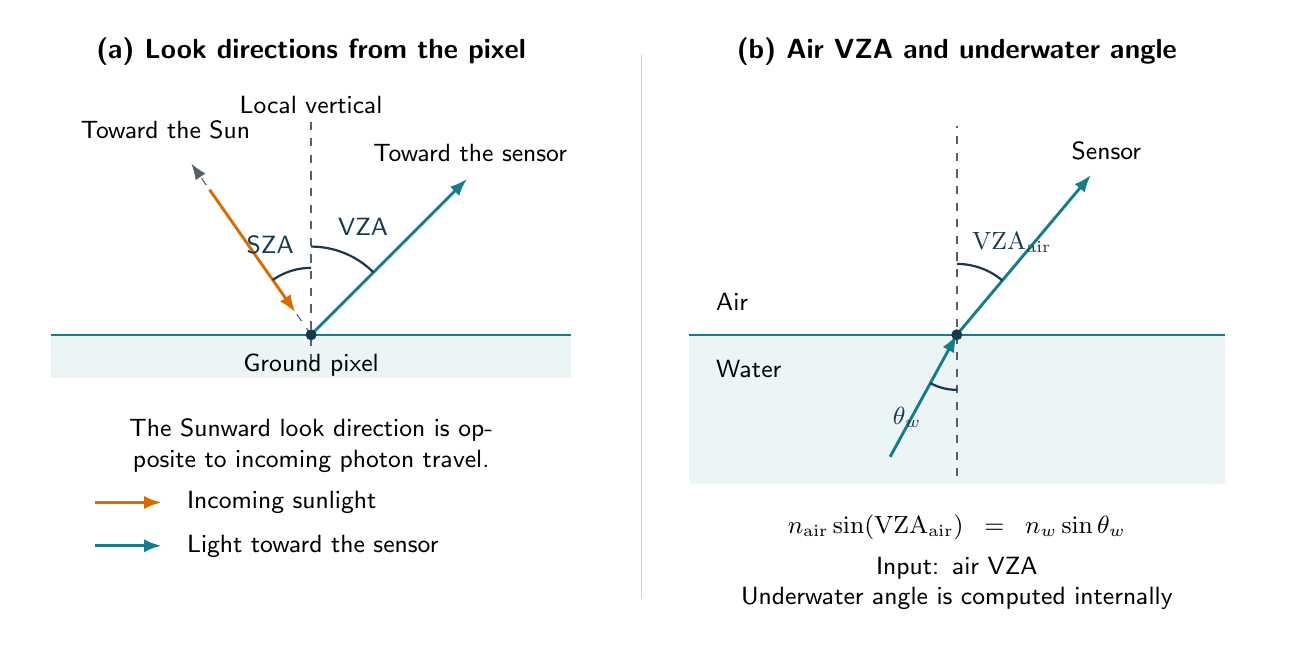
\begin{tikzpicture}[x=1cm,y=1cm,font=\sffamily\fontsize{9}{11}\selectfont,
  ray/.style={line width=1.05pt,-{Latex[length=2.2mm]}},
  axis/.style={ocrtGray,dashed,line width=.55pt},
  angle/.style={ocrtNavy,line width=.8pt},
  note/.style={align=center,text width=6.8cm}]
\path[use as bounding box] (0,-3.6) rectangle (15.8,3.9);
\begin{scope}[shift={(3.6,0)}]
  \node[anchor=north,font=\sffamily\bfseries] at (0,3.9)
    {\FigLang{(a) 화소에서 위쪽을 바라본 각도}{(a) Look directions from the pixel}};
  \fill[ocrtTeal!8] (-3.3,-.55) rectangle (3.3,0);
  \draw[ocrtTeal,line width=.8pt] (-3.3,0)--(3.3,0);
  \draw[axis] (0,-.35)--(0,2.75);
  \node[anchor=south,fill=white,inner sep=1.5pt] at (0,2.75)
    {\FigLang{국소 수직선}{Local vertical}};
  \draw[ocrtGray,dashed,-{Latex[length=2mm]}] (0,0)--(125:2.65);
  \draw[ray,orange!85!black] (125:2.25)--(125:.35);
  \draw[ray,ocrtTeal] (0,0)--(45:2.8);
  \node[anchor=south,align=center] at (-1.85,2.37)
    {\FigLang{태양을 향한 방향}{Toward the Sun}};
  \node[anchor=south,align=center] at (2.02,2.08)
    {\FigLang{센서를 향한 방향}{Toward the sensor}};
  \draw[angle] (90:.85) arc[start angle=90,end angle=125,radius=.85];
  \node[ocrtNavy] at (-.52,1.14) {SZA};
  \draw[angle] (45:1.12) arc[start angle=45,end angle=90,radius=1.12];
  \node[ocrtNavy] at (.66,1.37) {VZA};
  \fill[ocrtNavy] (0,0) circle (2pt);
  \node[anchor=north] at (0,-.12) {\FigLang{지상 화소}{Ground pixel}};
  \node[note,anchor=north] at (0,-.95)
    {\FigLang{태양을 바라보는 방향과 입사광의 진행 방향은 서로 반대다.}{The Sunward look direction is opposite to incoming photon travel.}};
  \draw[ray,orange!85!black] (-2.75,-2.13)--(-1.9,-2.13);
  \node[anchor=west] at (-1.7,-2.13) {\FigLang{입사 태양광}{Incoming sunlight}};
  \draw[ray,ocrtTeal] (-2.75,-2.68)--(-1.9,-2.68);
  \node[anchor=west] at (-1.7,-2.68) {\FigLang{센서로 나가는 빛}{Light toward the sensor}};
\end{scope}
\draw[ocrtLine] (7.8,-3.35)--(7.8,3.55);
\begin{scope}[shift={(11.8,0)}]
  \node[anchor=north,font=\sffamily\bfseries] at (0,3.9)
    {\FigLang{(b) 공기 중 VZA와 수중 각도}{(b) Air VZA and underwater angle}};
  \fill[ocrtTeal!8] (-3.4,-1.9) rectangle (3.4,0);
  \draw[ocrtTeal,line width=.8pt] (-3.4,0)--(3.4,0);
  \draw[axis] (0,-1.8)--(0,2.65);
  \draw[ray,ocrtTeal] (-.847,-1.55)--(0,0);
  \draw[ray,ocrtTeal] (0,0)--(50:2.65);
  \node[anchor=south,align=center] at (1.9,2.1)
    {\FigLang{센서}{Sensor}};
  \node[anchor=west] at (-3.18,.42) {\FigLang{공기}{Air}};
  \node[anchor=west] at (-3.18,-.43) {\FigLang{물}{Water}};
  \draw[angle] (50:.9) arc[start angle=50,end angle=90,radius=.9];
  \node[ocrtNavy] at (.7,1.17) {$\mathrm{VZA}_{\rm air}$};
  \draw[angle] (-90:.7) arc[start angle=-90,end angle=-118.66,radius=.7];
  \node[ocrtNavy] at (-.63,-1.05) {$\theta_w$};
  \fill[ocrtNavy] (0,0) circle (2pt);
  \node[note,anchor=north] at (0,-2.16)
    {$n_{\rm air}\sin(\mathrm{VZA}_{\rm air})=n_w\sin\theta_w$};
  \node[note,anchor=north] at (0,-2.7)
    {\FigLang{입력: 공기 중 VZA\\수중 각도는 내부에서 계산}{Input: air VZA\\Underwater angle is computed internally}};
\end{scope}
\end{tikzpicture}
\caption{\FigLang{SZA와 VZA는 화소의 위쪽 수직선에서 잰다. (a)는 두 look 방향을 한 단면에 배치한 예시이며 일반 기하의 RAA는 별도로 지정한다. (b)는 평탄한 경계의 굴절 도식이다. 표준 해양 경로의 VZA 입력을 수중 각도로 바꾸어 넣지 않는다.}{SZA and VZA are measured from the upward vertical at the pixel. Panel (a) places both look directions in one cross-section for illustration; RAA is specified separately for general geometry. Panel (b) shows refraction at a flat interface. Do not replace the standard ocean-path air-VZA input with an underwater angle.}}
\label{fig:geometry-zenith-refraction}
\end{figure}

% Angles drawn from exact ray endpoints; exaggerated orbital height is schematic.
\begin{figure}[H]
\centering
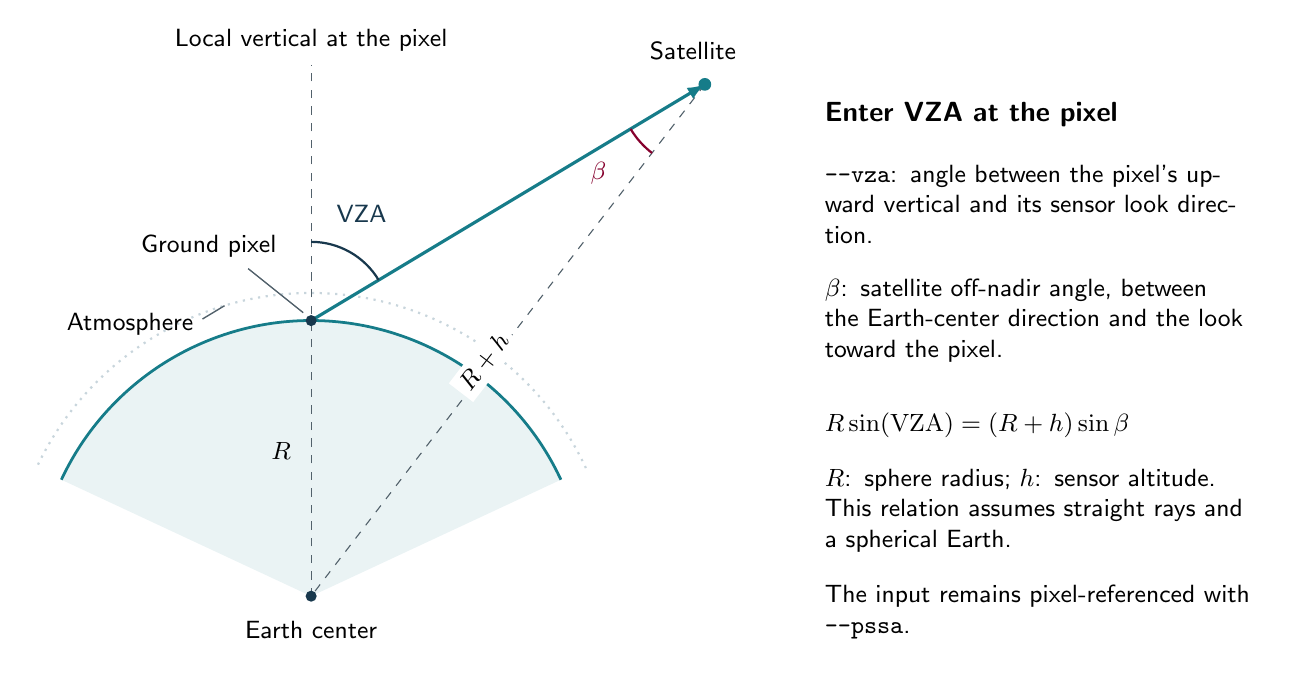
\begin{tikzpicture}[x=1cm,y=1cm,font=\sffamily\fontsize{9}{11}\selectfont,
  note/.style={align=left,text width=5.4cm}]
\path[use as bounding box] (0,-3.15) rectangle (15.8,4.72);
\coordinate (C) at (3.6,-2.5);
\coordinate (P) at (3.6,1);
\coordinate (S) at (8.6,4);
\fill[ocrtTeal!9] (C)--($(C)+(25:3.5)$)
  arc[start angle=25,end angle=155,radius=3.5]--cycle;
\draw[ocrtTeal,line width=1pt] ($(C)+(25:3.5)$)
  arc[start angle=25,end angle=155,radius=3.5];
\draw[ocrtLine,dotted,line width=.8pt] ($(C)+(25:3.85)$)
  arc[start angle=25,end angle=155,radius=3.85];
\draw[ocrtGray,dashed] (C)--(3.6,4.25);
\draw[ocrtGray,dashed] (S)--(C);
\draw[ocrtTeal,line width=1.15pt,-{Latex[length=2.2mm]}] (P)--(S);
\draw[ocrtNavy,line width=.8pt] ($(P)+(30.96376:1)$)
  arc[start angle=30.96376,end angle=90,radius=1];
\node[ocrtNavy,fill=white,inner sep=1pt] at (4.24,2.36) {VZA};
\draw[purple!70!black,line width=.8pt] ($(S)+(-149.03624:1.1)$)
  arc[start angle=-149.03624,end angle=-127.56859,radius=1.1];
\node[purple!70!black,fill=white,inner sep=1pt] at (7.25,2.87) {$\beta$};
\fill[ocrtNavy] (P) circle (2pt);
\fill[ocrtNavy] (C) circle (2pt);
\fill[ocrtTeal] (S) circle (2.3pt);
\node[anchor=south,align=center] at (3.6,4.29)
  {\FigLang{화소의 국소 수직선}{Local vertical at the pixel}};
\node[anchor=south,align=center] at (8.45,4.19)
  {\FigLang{위성}{Satellite}};
\node[align=center] at (2.3,1.95)
  {\FigLang{지상 화소}{Ground pixel}};
\draw[ocrtGray,line width=.5pt] (2.8,1.66)--(3.5,1.1);
\node[anchor=north,align=center] at (3.6,-2.69)
  {\FigLang{지구 중심}{Earth center}};
\node[align=center] at (1.3,.95)
  {\FigLang{대기층}{Atmosphere}};
\draw[ocrtGray,line width=.5pt] (2.22,1.02)--(2.5,1.189);
\node[fill=ocrtTeal!9,inner sep=2pt] at (3.22,-.65) {$R$};
\node[rotate=52.43,fill=white,inner sep=2pt] at (5.8,.47) {$R+h$};
\node[anchor=north west,note,font=\sffamily\bfseries] at (10.0,3.9)
  {\FigLang{입력하는 각도는 VZA}{Enter VZA at the pixel}};
\node[anchor=north west,note] at (10.0,3.1)
  {\FigLang{\texttt{--vza}: 화소의 위쪽 수직선과 센서 look 방향 사이의 각도.}{\texttt{--vza}: angle between the pixel's upward vertical and its sensor look direction.}};
\node[anchor=north west,note] at (10.0,1.65)
  {\FigLang{$\beta$: 위성에서 지구 중심을 향하는 천저 방향과 화소를 향하는 방향 사이의 off-nadir 각도.}{$\beta$: satellite off-nadir angle, between the Earth-center direction and the look toward the pixel.}};
\node[anchor=north west,note] at (10.0,-.05)
  {$R\sin(\mathrm{VZA})=(R+h)\sin\beta$};
\node[anchor=north west,note] at (10.0,-.76)
  {\FigLang{$R$: 구의 반지름, $h$: 센서 고도. 직선 광선·구형 지구에서의 기하 관계다.}{$R$: sphere radius; $h$: sensor altitude. This relation assumes straight rays and a spherical Earth.}};
\node[anchor=north west,note] at (10.0,-2.24)
  {\FigLang{\texttt{--pssa}에서도 입력 기준은 화소다.}{The input remains pixel-referenced with \texttt{--pssa}.}};
\end{tikzpicture}
\caption{\FigLang{구면 기하에서 지상 화소의 VZA와 위성의 off-nadir 각도는 일반적으로 다르다. 대기층 두께와 센서 고도는 구별이 쉽도록 과장했으며 비례도·계산 결과가 아니다. 현재 \texttt{--pssa}의 IPSS 보정도 지상 화소 기준 기하를 사용한다. 이 도식은 완전한 3차원 구면 다중산란 모델을 의미하지 않는다.}{In spherical geometry, ground-pixel VZA and satellite off-nadir angle generally differ. Atmospheric thickness and sensor altitude are exaggerated for clarity; this is not a scale drawing or a computed result. The current IPSS correction enabled by \texttt{--pssa} also uses ground-pixel geometry. The schematic does not imply a fully three-dimensional spherical multiple-scattering model.}}
\label{fig:geometry-curvature}
\end{figure}


\section{Operational definition of OCRT RAA}
\label{sec:auto:01_concepts_geometry:4}
\textbf{The direct sunglint direction in OCRT is \texttt{RAA=\allowbreak{}180\textdegree{}}.} For specular reflection from a flat surface, this is the specular branch when \texttt{SZA=\allowbreak{}VZA}. Wind broadens the specular signal into neighboring angles through the Cox--Munk slope distribution.


{\TableFont
\begin{longtable}{@{}>{\raggedright\arraybackslash}p{\dimexpr 0.3400\linewidth-4.00pt\relax}>{\raggedright\arraybackslash}p{\dimexpr 0.6600\linewidth-4.00pt\relax}@{}}
\toprule
\textbf{OCRT RAA} & \textbf{Interpretation} \\
\midrule
\endfirsthead
\toprule
\textbf{OCRT RAA} & \textbf{Interpretation} \\
\midrule
\endhead
\bottomrule
\endfoot
\texttt{0\textdegree{}} & Principal-plane branch opposite direct glint \\
\texttt{90\textdegree{}} & One azimuth perpendicular to the principal plane \\
\texttt{180\textdegree{}} & Direct-glint principal-plane branch; specular geometry when \texttt{SZA=\allowbreak{}VZA} \\
\texttt{270\textdegree{}} & Mirror azimuth of \texttt{90\textdegree{}}; \texttt{I/\allowbreak{}Q} are symmetric, while \texttt{U} can have the opposite sign \\
\texttt{360\textdegree{}} & Same direction as \texttt{0\textdegree{}} \\
\end{longtable}
}

Do not determine RAA from descriptions such as “on the same side as the Sun,” “forward,” or “backward” alone. The direction \textbf{looking toward the Sun} and the direction in which sunlight \textbf{propagates} differ by 180\textdegree{} in horizontal azimuth. If another radiative transfer code or LUT places glint at \texttt{RAA=\allowbreak{}0\textdegree{}}, that numerical value cannot be used directly in OCRT.

Following solar photon travel and the sensor look direction in Figure~\ref{fig:geometry-glint-branches} makes the two branches easier to distinguish. The \texttt{RAA=180\textdegree{}} branch alone does not define the specular center: \texttt{SZA=VZA} is also required.

% Equal 30-degree zenith angles. Solar-look and propagation vectors differ.
\begin{figure}[H]
\centering
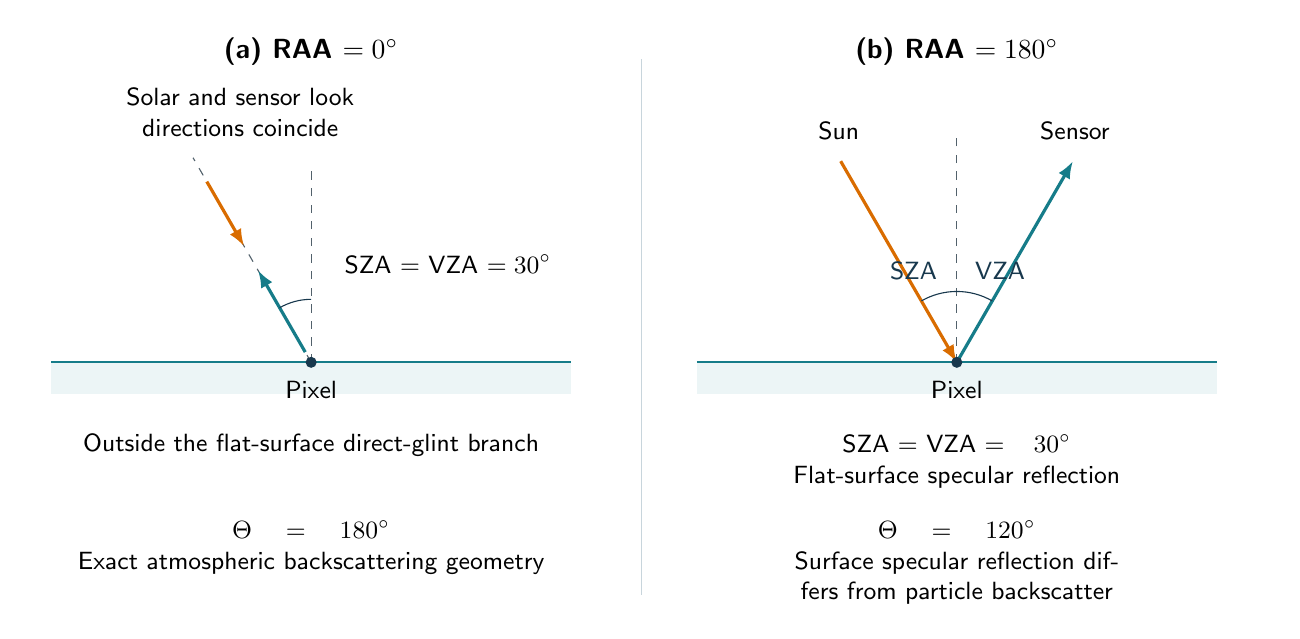
\begin{tikzpicture}[x=1cm,y=1cm,font=\sffamily\fontsize{9}{11}\selectfont,
  ray/.style={line width=1.15pt,-{Latex[length=2.2mm]}},
  note/.style={align=center,text width=6.9cm}]
\path[use as bounding box] (0,-3.15) rectangle (15.8,4.25);
\begin{scope}[shift={(3.6,0)}]
  \node[anchor=north,font=\sffamily\bfseries] at (0,4.25)
    {(a) RAA $=0^\circ$};
  \fill[ocrtTeal!8] (-3.3,-.4) rectangle (3.3,0);
  \draw[ocrtTeal,line width=.8pt] (-3.3,0)--(3.3,0);
  \draw[ocrtGray,dashed] (0,0)--(0,2.45);
  \draw[ocrtGray,dashed] (0,0)--(120:3.0);
  \draw[ray,orange!85!black] (120:2.65)--(120:1.7);
  \draw[ray,ocrtTeal] (120:.15)--(120:1.35);
  \node[anchor=south,align=center,text width=4.8cm] at (-.9,2.75)
    {\FigLang{태양과 센서의 look 방향 일치}{Solar and sensor look directions coincide}};
  \draw[ocrtNavy] (90:.8) arc[start angle=90,end angle=120,radius=.8];
  \node[anchor=west,align=left] at (.3,1.25)
    {SZA $=$ VZA $=30^\circ$};
  \fill[ocrtNavy] (0,0) circle (2pt);
  \node[anchor=north] at (0,-.12) {\FigLang{화소}{Pixel}};
  \node[note,anchor=north] at (0,-.79)
    {\FigLang{평탄면의 직접 글린트 가지가 아님}{Outside the flat-surface direct-glint branch}};
  \node[note,anchor=north] at (0,-1.88)
    {$\Theta=180^\circ$\\\FigLang{대기 입자의 정확 후방산란 기하}{Exact atmospheric backscattering geometry}};
\end{scope}
\draw[ocrtLine] (7.8,-2.95)--(7.8,3.85);
\begin{scope}[shift={(11.8,0)}]
  \node[anchor=north,font=\sffamily\bfseries] at (0,4.25)
    {(b) RAA $=180^\circ$};
  \fill[ocrtTeal!8] (-3.3,-.4) rectangle (3.3,0);
  \draw[ocrtTeal,line width=.8pt] (-3.3,0)--(3.3,0);
  \draw[ocrtGray,dashed] (0,0)--(0,2.85);
  \draw[ray,orange!85!black] (120:2.95)--(0,0);
  \draw[ray,ocrtTeal] (0,0)--(60:2.95);
  \node[anchor=south] at (-1.5,2.7) {\FigLang{태양}{Sun}};
  \node[anchor=south] at (1.5,2.7) {\FigLang{센서}{Sensor}};
  \draw[ocrtNavy] (90:.9) arc[start angle=90,end angle=120,radius=.9];
  \draw[ocrtNavy] (60:.9) arc[start angle=60,end angle=90,radius=.9];
  \node[ocrtNavy] at (-.55,1.16) {SZA};
  \node[ocrtNavy] at (.55,1.16) {VZA};
  \fill[ocrtNavy] (0,0) circle (2pt);
  \node[anchor=north] at (0,-.12) {\FigLang{화소}{Pixel}};
  \node[note,anchor=north] at (0,-.79)
    {SZA $=$ VZA $=30^\circ$\\\FigLang{평탄면 정반사}{Flat-surface specular reflection}};
  \node[note,anchor=north] at (0,-1.88)
    {$\Theta=120^\circ$\\\FigLang{수면 정반사와 입자 후방산란은 구별}{Surface specular reflection differs from particle backscatter}};
\end{scope}
\end{tikzpicture}
\caption{\FigLang{두 주평면 가지를 같은 천정각으로 비교한 단면도. 주황 화살표는 입사광, 청록 화살표는 센서 방향으로 나가는 빛이다. (a)의 두 화살표는 같은 직선 위에서 서로 반대 방향을 가리킨다. $\Theta$는 입사 태양광의 진행 방향과 상향 관측 방향 사이의 대기 산란각이며 수면 법선에서 잰 각도가 아니다. 바람이 있는 해수면의 글린트는 (b)의 중심 주변으로 넓어질 수 있다.}{Cross-sections comparing the two principal-plane branches at equal zenith angles. Orange arrows show incoming photons and teal arrows show light toward the sensor. The arrows in (a) point in opposite directions on the same line. $\Theta$ is the atmospheric scattering angle between incoming solar propagation and upward viewing, not an angle measured from the surface normal. A wind-roughened surface can broaden glint around the center shown in (b).}}
\label{fig:geometry-glint-branches}
\end{figure}


\subsection{Calculation from satellite SAA/VAA}
\label{sec:auto:01_concepts_geometry:4.1}
First check the following in the product metadata.

\begin{enumerate}
\item Verify that SAA is the azimuth \textbf{toward the Sun} from the ground pixel.
\item Verify that VAA is the azimuth \textbf{toward the sensor} from the ground pixel. If it is the azimuth from the sensor toward the surface, add \texttt{180\textdegree{}} to convert it to a ground-pixel reference.
\item Align the zero reference and positive rotation direction of SAA and VAA. Do not repeat this procedure on a value already supplied as a relative azimuth angle.
\end{enumerate}

When both values satisfy these look-azimuth definitions and use the same rotation direction, the following is an explicit conversion convention consistent with OCRT's \texttt{0/\allowbreak{}180\textdegree{}} branches.


\begin{ManualCode}
def ocrt_raa_from_look_azimuths(saa_deg, vaa_deg):
    return (vaa_deg - saa_deg) % 360.0
\end{ManualCode}


{\TableFont
\begin{longtable}{@{}>{\raggedright\arraybackslash}p{\dimexpr 0.2300\linewidth-6.00pt\relax}>{\raggedright\arraybackslash}p{\dimexpr 0.2400\linewidth-6.00pt\relax}>{\raggedright\arraybackslash}p{\dimexpr 0.2300\linewidth-6.00pt\relax}>{\raggedright\arraybackslash}p{\dimexpr 0.3000\linewidth-6.00pt\relax}@{}}
\toprule
\textbf{SAA} & \textbf{VAA} & \textbf{OCRT RAA from the equation above} & \textbf{Meaning} \\
\midrule
\endfirsthead
\toprule
\textbf{SAA} & \textbf{VAA} & \textbf{OCRT RAA from the equation above} & \textbf{Meaning} \\
\midrule
\endhead
\bottomrule
\endfoot
30\textdegree{} & 30\textdegree{} & 0\textdegree{} & Solar look azimuth and sensor look azimuth coincide \\
30\textdegree{} & 210\textdegree{} & 180\textdegree{} & Glint branch; the specular center also requires SZA=VZA \\
350\textdegree{} & 10\textdegree{} & 20\textdegree{} & Difference crossing the 0\textdegree{} boundary \\
10\textdegree{} & 350\textdegree{} & 340\textdegree{} & Mirror azimuth of the preceding row \\
\end{longtable}
}

This equation is a transformation derived in the coordinates declared above; it does not automatically align the Stokes reference plane of a particular satellite product. Reversing the product's positive azimuth rotation direction changes \texttt{RAA} to \texttt{360-RAA}, reversing the sign of \texttt{U} even when \texttt{I/\allowbreak{}Q} remain the same. For polarized data, record the original SAA/VAA, conversion equation, reference plane, and rotation direction together, and compare signed \texttt{U} at an off-principal-plane geometry. If the product's azimuth and Stokes definitions are unknown, agreement in \texttt{I/\allowbreak{}Q} alone does not validate the \texttt{U} transformation.

Figure~\ref{fig:geometry-azimuth} shows the rotation from SAA to VAA. The right panel rotates the same coordinates to the solar look azimuth and illustrates why mirror azimuths need to remain distinguishable in stored data.

% Clockwise is an explicitly declared illustrative coordinate convention.
\begin{figure}[H]
\centering
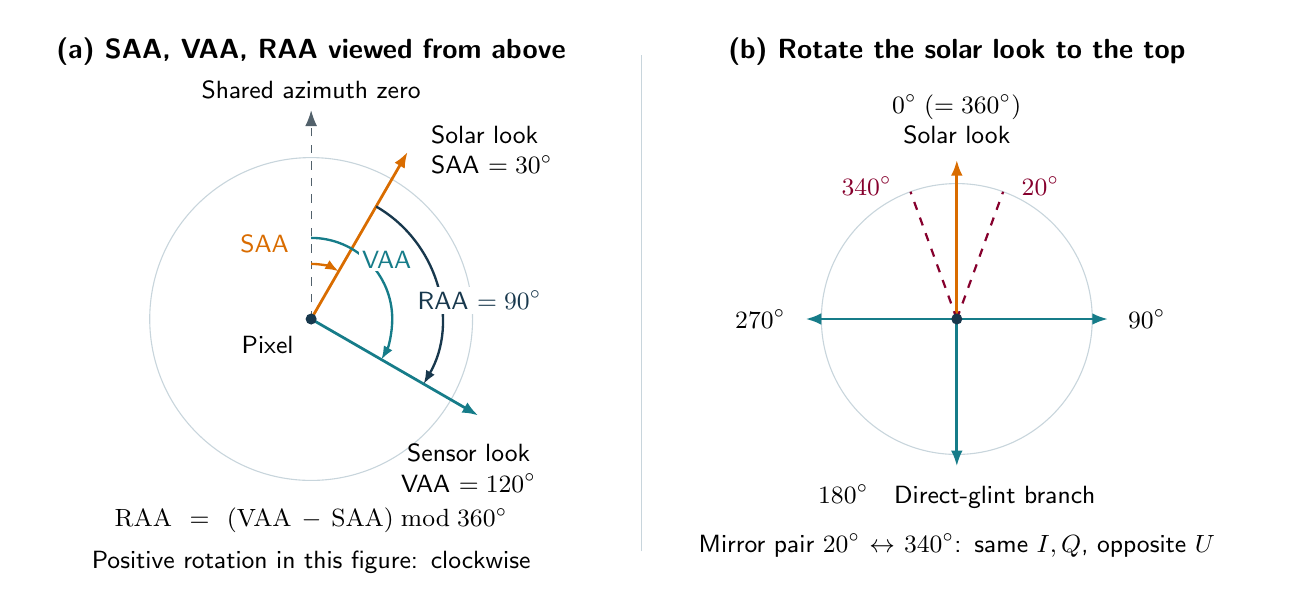
\begin{tikzpicture}[x=1cm,y=1cm,font=\sffamily\fontsize{9}{11}\selectfont,
  ray/.style={line width=1pt,-{Latex[length=2mm]}},
  arcarr/.style={line width=.85pt,-{Latex[length=1.7mm]}},
  note/.style={align=center,text width=6.9cm}]
\path[use as bounding box] (0,-3.1) rectangle (15.8,3.7);
\begin{scope}[shift={(3.6,0)}]
  \node[anchor=north,font=\sffamily\bfseries] at (0,3.7)
    {\FigLang{(a) 위에서 본 SAA, VAA, RAA}{(a) SAA, VAA, RAA viewed from above}};
  \draw[ocrtLine] (0,0) circle (2.05);
  \draw[ocrtGray,dashed,-{Latex[length=2mm]}] (0,0)--(0,2.65);
  \node[anchor=south,align=center] at (0,2.68)
    {\FigLang{공통 방위 영점}{Shared azimuth zero}};
  \draw[ray,orange!85!black] (0,0)--(60:2.45);
  \draw[ray,ocrtTeal] (0,0)--(-30:2.45);
  \node[anchor=west,align=left] at (1.4,2.15)
    {\FigLang{태양 look}{Solar look}\\SAA $=30^\circ$};
  \node[anchor=north,align=center] at (2.0,-1.47)
    {\FigLang{센서 look}{Sensor look}\\VAA $=120^\circ$};
  \draw[arcarr,orange!85!black] (90:.7) arc[start angle=90,end angle=60,radius=.7];
  \node[anchor=east,orange!85!black] at (-.16,.95) {SAA};
  \draw[arcarr,ocrtTeal] (90:1.03) arc[start angle=90,end angle=-30,radius=1.03];
  \node[ocrtTeal,fill=white,inner sep=1pt] at (.96,.75) {VAA};
  \draw[arcarr,ocrtNavy] (60:1.65) arc[start angle=60,end angle=-30,radius=1.65];
  \node[ocrtNavy,fill=white,inner sep=1.5pt] at (2.14,.24) {RAA $=90^\circ$};
  \fill[ocrtNavy] (0,0) circle (2pt);
  \node[anchor=north east] at (-.1,-.1) {\FigLang{화소}{Pixel}};
  \node[note,anchor=north] at (0,-2.28)
    {$\mathrm{RAA}=(\mathrm{VAA}-\mathrm{SAA})\bmod 360^\circ$};
  \node[note,anchor=north] at (0,-2.83)
    {\FigLang{이 그림의 양의 회전: 시계 방향}{Positive rotation in this figure: clockwise}};
\end{scope}
\draw[ocrtLine] (7.8,-2.95)--(7.8,3.35);
\begin{scope}[shift={(11.8,0)}]
  \node[anchor=north,font=\sffamily\bfseries] at (0,3.7)
    {\FigLang{(b) 태양 look을 위쪽으로 맞춘 좌표}{(b) Rotate the solar look to the top}};
  \draw[ocrtLine] (0,0) circle (1.72);
  \draw[ray,orange!85!black] (0,0)--(0,2.02);
  \draw[ray,ocrtTeal] (0,0)--(1.92,0);
  \draw[ray,ocrtTeal] (0,0)--(0,-1.87);
  \draw[ray,ocrtTeal] (0,0)--(-1.92,0);
  \draw[purple!70!black,dashed,line width=.8pt] (0,0)--(70:1.72);
  \draw[purple!70!black,dashed,line width=.8pt] (0,0)--(110:1.72);
  \node[purple!70!black,anchor=west] at (.7,1.69) {$20^\circ$};
  \node[purple!70!black,anchor=east] at (-.7,1.69) {$340^\circ$};
  \node[anchor=south,align=center] at (0,2.1)
    {$0^\circ\;(=360^\circ)$\\\FigLang{태양 look}{Solar look}};
  \node[anchor=west] at (2.05,0) {$90^\circ$};
  \node[anchor=east] at (-2.05,0) {$270^\circ$};
  \node[anchor=north,align=center] at (0,-1.98)
    {$180^\circ$\quad\FigLang{직접 글린트 가지}{Direct-glint branch}};
  \fill[ocrtNavy] (0,0) circle (2pt);
  \node[note,anchor=north] at (0,-2.6)
    {\FigLang{거울 방위 $20^\circ\leftrightarrow340^\circ$: 같은 $I,Q$, 반대 $U$}{Mirror pair $20^\circ\leftrightarrow340^\circ$: same $I,Q$, opposite $U$}};
\end{scope}
\end{tikzpicture}
\caption{\FigLang{위에서 본 수평 look 방위의 차이로 RAA를 정한다. 영점과 시계 방향은 이 그림에서 선택한 규약이다. 제품의 SAA/VAA를 같은 영점·회전 방향으로 맞춘 후 변환한다. 축대칭 조건에서 $20^\circ$와 $340^\circ$를 모두 $20^\circ$로 접으면 signed $U$에 필요한 거울 방향 정보가 사라진다. 실제 편광 비교에는 Stokes 기준면도 맞춘다.}{RAA is the difference between horizontal look azimuths viewed from above. The zero reference and clockwise rotation are choices declared for this figure. Align the product's SAA/VAA origins and rotation directions before conversion. Under axisymmetric conditions, folding both $20^\circ$ and $340^\circ$ to $20^\circ$ discards the mirror-direction information needed for signed $U$. Polarization comparisons also require aligned Stokes reference planes.}}
\label{fig:geometry-azimuth}
\end{figure}


\subsection{When only RAA folded into 0--180\textdegree{} is available}
\label{sec:auto:01_concepts_geometry:4.2}
A folded value is commonly generated as follows.


\begin{ManualCode}
raa_360 = (vaa_deg - saa_deg) % 360.0
raa_folded = min(raa_360, 360.0 - raa_360)
\end{ManualCode}

Under axisymmetric conditions, a half-circle grid can be used for LUTs containing only \texttt{I} and \texttt{Q}. However, retaining only \texttt{raa\_\allowbreak{}folded=\allowbreak{}20\textdegree{}} loses whether the original direction was \texttt{20\textdegree{}} or \texttt{340\textdegree{}}. To preserve \texttt{U}, also store the original 0--360\textdegree{} direction or an indication of the mirror direction. Storing the absolute value \texttt{abs(U)} discards directional information.

\section{Matching Phi in other codes}
\label{sec:auto:01_concepts_geometry:5}
The current \texttt{rt\_\allowbreak{}raa\_\allowbreak{}convention.\allowbreak{}h} defines \textbf{one of the following two equivalent alternatives} for OCRT--OSOAA comparisons.


{\TableFont
\begin{longtable}{@{}>{\raggedright\arraybackslash}p{\dimexpr 0.3000\linewidth-5.33pt\relax}>{\raggedright\arraybackslash}p{\dimexpr 0.2300\linewidth-5.33pt\relax}>{\raggedright\arraybackslash}p{\dimexpr 0.4700\linewidth-5.33pt\relax}@{}}
\toprule
\textbf{Conversion method} & \textbf{Azimuth passed to OSOAA} & \textbf{U comparison with OCRT} \\
\midrule
\endfirsthead
\toprule
\textbf{Conversion method} & \textbf{Azimuth passed to OSOAA} & \textbf{U comparison with OCRT} \\
\midrule
\endhead
\bottomrule
\endfoot
A & \texttt{Phi\_\allowbreak{}OSOAA=\allowbreak{}(180-RAA\_\allowbreak{}OCRT) mod 360} & \texttt{U\_\allowbreak{}OCRT=\allowbreak{}-U\_\allowbreak{}OSOAA} \\
B & \texttt{Phi\_\allowbreak{}OSOAA=\allowbreak{}(RAA\_\allowbreak{}OCRT+180) mod 36\allowbreak{}0} & \texttt{U\_\allowbreak{}OCRT=\allowbreak{}U\_\allowbreak{}OSOAA} \\
\end{longtable}
}

Both methods construct the same physical comparison for \texttt{I/\allowbreak{}Q}. Do not apply method A's U sign reversal together with method B's angle transformation. This rule assumes the output conventions of the corresponding comparison harness; it is not a universal formula for arbitrary codes.

Current OCRT atmospheric outputs, above-surface \texttt{Rrs}, and below-surface \texttt{rrs} are Fourier-reconstructed using \textbf{the same public RAA}. The historical no-conversion rule \texttt{Phi\_\allowbreak{}OSOAA,\allowbreak{}water=\allowbreak{}RAA\_\allowbreak{}OCRT} corresponded to water outputs before the correction. Do not use it for water outputs from the current source.

When reading a CCRR reference CSV, \texttt{-\allowbreak{}-\allowbreak{}ccrr-\allowbreak{}compare} internally applies \texttt{RAA\_\allowbreak{}OCRT=\allowbreak{}(180-RAA\_\allowbreak{}CCRR) mod 360}. If the CSV's \texttt{raa\_\allowbreak{}deg} already follows the OCRT convention, do not feed it directly into this comparison mode and transform it twice. Check \texttt{raa\_\allowbreak{}ccrr\_\allowbreak{}deg}, \texttt{raa\_\allowbreak{}ocrt\_\allowbreak{}deg}, and \texttt{raa\_\allowbreak{}mapping} in the results.

\section{Stokes signs and off-principal-plane validation}
\label{sec:auto:01_concepts_geometry:6}
The public default path uses Stokes components aligned with the viewing-direction meridian plane (the plane containing the viewing direction and the vertical). The default surface Q convention is \texttt{q\_\allowbreak{}convention=\allowbreak{}1}, with the Fresnel core component \texttt{Q\_\allowbreak{}kernel=\allowbreak{}(Rp-Rs)/\allowbreak{}2}. \texttt{Q} and \texttt{U} are signed quantities, and negative values are normal. Comparison with sensor coordinates or scattering-plane coordinates may require a reference-plane rotation.

For an axisymmetric surface and medium, using the same reference plane, the following symmetries hold.


\begin{ManualCode}
I(RAA) =  I(360−RAA)
Q(RAA) =  Q(360−RAA)
U(RAA) = −U(360−RAA)
\end{ManualCode}

In the principal plane at \texttt{RAA=\allowbreak{}0/\allowbreak{}180\textdegree{}}, U is zero or at the numerical-error level, so errors in the U sign are not exposed. Also check off-principal-plane pairs such as \texttt{RAA=\allowbreak{}45/\allowbreak{}315\textdegree{}}. At exactly \texttt{VZA=\allowbreak{}0\textdegree{}}, the meridian plane is geometrically degenerate, so Q/U as a function of RAA may not correspond to intuitive left/right directions. Include small positive VZA values in model comparisons rather than using only nadir values.

\section{Scattering angle and conflicting historical comments}
\label{sec:auto:01_concepts_geometry:7}
Taking the dot product of the actual solar propagation vector and the upward viewing vector derived from the look directions declared above gives the atmospheric scattering angle:


\begin{ManualCode}
mu_s = cos(SZA), mu_v = cos(VZA)
cos(Theta) = −mu_s*mu_v − sin(SZA)*sin(VZA)*cos(RAA_OCRT)
\end{ManualCode}

This matches the expression currently used by \texttt{rt\_\allowbreak{}ipss\_\allowbreak{}cos\_\allowbreak{}scattering\_\allowbreak{}angle()}. For \texttt{SZA=\allowbreak{}VZA=\allowbreak{}30\textdegree{}}, \texttt{Theta=\allowbreak{}180\textdegree{}} at \texttt{RAA=\allowbreak{}0\textdegree{}}, whereas \texttt{Theta=\allowbreak{}120\textdegree{}} at the glint branch, \texttt{RAA=\allowbreak{}180\textdegree{}}. \textbf{The surface specular-reflection direction and exact backscattering by atmospheric particles are different concepts.}

The current repository also contains an unresolved inconsistency in its internal descriptions. The helper \texttt{rt\_\allowbreak{}atm\_\allowbreak{}scatter\_\allowbreak{}cos\_\allowbreak{}from\_\allowbreak{}public\_\allowbreak{}raa()} in \texttt{rt\_\allowbreak{}raa\_\allowbreak{}convention.\allowbreak{}h} uses \texttt{+sin(SZA)*sin(VZ\allowbreak{}A)*cos(RAA)}, opposite to the sign above, and associated comments and \texttt{test\_\allowbreak{}raa\_\allowbreak{}convention.\allowbreak{}c} describe \texttt{RAA=\allowbreak{}180\textdegree{}} as exact backscattering. At the time this manual was prepared, no production \texttt{src} calls to this helper were found; actual Fourier reconstruction uses \texttt{public\_\allowbreak{}RAA+\ensuremath{\pi}}, and IPSS uses the \texttt{-cos(RAA)} expression above. Therefore, do not use this helper or the “exact backscattering” wording in historical audit reports as the basis for satellite-geometry conversion. This manual does not change the source code.

\subsection{Implementation references}
\label{sec:auto:01_concepts_geometry:7.1}
\begin{itemize}
\item \href{https://github.com/brtnt/OCRT/blob/54861c68e35ec5aaa3938fad53e93dc2dfa7eb1d/code/OCRT_C/src/rt_raa_convention.h}{Public RAA helpers and current OSOAA mapping}
\item \href{https://github.com/brtnt/OCRT/blob/54861c68e35ec5aaa3938fad53e93dc2dfa7eb1d/code/OCRT_C/src/rt_fourier.c}{Internal +\ensuremath{\pi} conversion in Fourier reconstruction}
\item \href{https://github.com/brtnt/OCRT/blob/54861c68e35ec5aaa3938fad53e93dc2dfa7eb1d/code/OCRT_C/src/rt_ipss.c}{IPSS scattering angle and pixel-referenced geometry}
\item \href{https://github.com/brtnt/OCRT/blob/54861c68e35ec5aaa3938fad53e93dc2dfa7eb1d/code/OCRT_C/src/main.c}{CLI mode selection and CCRR conversion}
\item \href{https://github.com/brtnt/OCRT/blob/54861c68e35ec5aaa3938fad53e93dc2dfa7eb1d/code/OCRT_C/src/shared/surface.c}{Surface Stokes components and meridian-plane rotation}
\end{itemize}

Before changing input parameters, first align these three features: glint at \texttt{RAA=\allowbreak{}180\textdegree{}}, the opposite branch at \texttt{0\textdegree{}}, and the off-principal-plane U sign. This reduces common 180\textdegree{} and sign errors in comparisons.


% Authoritative LaTeX chapter. Edit this file for future revisions.
% Initially migrated 2026-09-11; no Markdown import occurs during PDF builds.
\chapter{Installation and First Run}
\label{chap:02_installation}
Contents · \hyperref[chap:03_options]{Next: C options}

\section{Components and prerequisites}
\label{sec:auto:02_installation:1}
The recommended starting point is the C reference implementation. It requires a C11-capable GCC, OpenMP, and Git. The repository's Linux guidance specifies GCC 11 or later; Windows uses MinGW-w64 GCC. See \hyperref[chap:06_python_batch]{Appendix~\ref*{chap:06_python_batch}} for the Python batch package's dependencies and supported scope.


{\TableFont
\begin{longtable}{@{}>{\raggedright\arraybackslash}p{\dimexpr 0.3400\linewidth-4.00pt\relax}>{\raggedright\arraybackslash}p{\dimexpr 0.6600\linewidth-4.00pt\relax}@{}}
\toprule
\textbf{Location} & \textbf{Role} \\
\midrule
\endfirsthead
\toprule
\textbf{Location} & \textbf{Role} \\
\midrule
\endhead
\bottomrule
\endfoot
\texttt{code/\allowbreak{}OCRT\_\allowbreak{}C/\allowbreak{}src/\allowbreak{}} & C source \\
\texttt{code/\allowbreak{}OCRT\_\allowbreak{}C/\allowbreak{}inputs/\allowbreak{}} & AFGL, absorption cross sections, seawater IOPs, and Mie data read by C \\
\texttt{code/\allowbreak{}OCRT\_\allowbreak{}C/\allowbreak{}build/\allowbreak{}} & Executables built locally \\
\texttt{code/\allowbreak{}OCRT\_\allowbreak{}Python/\allowbreak{}} & Python implementation \\
\texttt{scripts/\allowbreak{}} & Public Mie data installers and hash lists \\
\end{longtable}
}

The command examples assume that the repository is cloned into a folder named \texttt{OCRT}. They do not hard-code absolute paths that vary by account or computer.


\par\noindent\begin{minipage}{\linewidth}
\begin{ManualCode}
git clone https://github.com/brtnt/OCRT.git
cd OCRT
git rev-parse HEAD
\end{ManualCode}
\end{minipage}\par

If the repository is already cloned, inspect any changes to the existing source and decide which version to use. Executables are not distributed through Git, so build after obtaining the source.

\section{Installing input data}
\label{sec:auto:02_installation:2}
Small data files are included in Git. The 181 FR631 Mie files needed for aerosol and particulate-ocean calculations are distributed in four archives in the \href{https://github.com/brtnt/OCRT/releases/tag/data-v1}{data-v1 release}. Allow approximately 1.3 GB for the download, approximately 4.3 GB for the C inputs, and approximately 4.3 GB for the Python copy. Also reserve space for the archive cache.

Run from the repository root.

Linux/Bash:


\par\noindent\begin{minipage}{\linewidth}
\begin{ManualCode}
bash scripts/fetch_data.sh
\end{ManualCode}
\end{minipage}\par

Windows/PowerShell:


\par\noindent\begin{minipage}{\linewidth}
\begin{ManualCode}
powershell -ExecutionPolicy Bypass -File scripts\fetch_data.ps1
\end{ManualCode}
\end{minipage}\par

The scripts verify the archives' SHA-256 hashes and install the data in the C and Python input folders. Do not use \texttt{-\allowbreak{}NoVerify} for a normal installation. Existing input files with the same names may be updated during installation, so keep modified user data separately.

To verify individual C Mie files on Linux as well:


\par\noindent\begin{minipage}{\linewidth}
\begin{ManualCode}
cd code/OCRT_C/inputs
sha256sum -c ../../../scripts/MIE_SHA256SUMS_data-v1.txt
cd ../../..
\end{ManualCode}
\end{minipage}\par

C Rayleigh examples without aerosols or underwater-particle calculations can be run without downloading the large Mie data set. Calculations with gas absorption enabled require the small AFGL and cross-section files. \textbf{Python has paths that preload additional data in constructors, so the C conditions for running without those data do not transfer directly to Python.}

\section{Building on Linux}
\label{sec:auto:02_installation:3}
The default CPU option in the \texttt{Makefile} is \texttt{-\allowbreak{}march=\allowbreak{}cascadelake} (AVX-512). Execution fails if the CPU does not support it. For a typical x86-64 AVX2 environment, specify the options explicitly:


\par\noindent\begin{minipage}{\linewidth}
\begin{ManualCode}
cd code/OCRT_C
make CFLAGS='-std=c11 -O3 -march=x86-64-v3 -ffp-contract=fast -fassociative-math -fno-signed-zeros -fno-trapping-math -DOCRT_FAST_KERNELS -fopenmp -Isrc'
./build/ocrt --version
./build/ocrt --help
\end{ManualCode}
\end{minipage}\par

When rebuilding with a different CPU option, force a rebuild with the same \textbf{complete} CFLAGS, for example \texttt{make -\allowbreak{}B CFLAGS=\allowbreak{}'\ldots{}'}. Replace \texttt{\ldots{}} in that command with the actual options. Make does not automatically regenerate an existing executable merely because CFLAGS changed.

An x86-64 CPU without AVX2 can use a build with \texttt{-\allowbreak{}march=\allowbreak{}x86-\allowbreak{}64}, but performance and numerical differences must be checked again. The x86-specific options above cannot be used on ARM/macOS, which is outside this manual's verified execution scope. Do not treat Apple Clang as equivalent to the GCC/OpenMP environment.

\section{Building on Windows}
\label{sec:auto:02_installation:4}
Install a GCC environment following the \href{https://www.msys2.org/}{official MSYS2 installation guidance}. The current official default environment is UCRT64. In a UCRT64 terminal, install GCC with:


\par\noindent\begin{minipage}{\linewidth}
\begin{ManualCode}
pacman -S mingw-w64-ucrt-x86_64-gcc
gcc --version
\end{ManualCode}
\end{minipage}\par

Existing OCRT Windows scripts were written for MinGW64 GCC. Consistently use the \texttt{bin} path of your MinGW64 or UCRT64 environment, and do not mix GCC/DLL environments. The following is \textbf{an example for UCRT64 with MSYS2 installed in its default location}. If your installation is elsewhere, change the corresponding PATH entry.

In PowerShell, starting at the repository root:


\par\noindent\begin{minipage}{\linewidth}
\begin{ManualCode}
$env:Path = 'C:\msys64\ucrt64\bin;' + $env:Path
gcc --version
Set-Location code\OCRT_C
.\build_win.bat
.\build\ocrt_x86-64-v3.exe --version
.\build\ocrt_x86-64-v3.exe --help
\end{ManualCode}
\end{minipage}\par

\texttt{build\_\allowbreak{}win.\allowbreak{}bat} includes the Windows compatibility source files, and its default output is \texttt{build\textbackslash{}ocrt\_\allowbreak{}x86-\allowbreak{}64-\allowbreak{}v3.\allowbreak{}exe}. It waits for a keypress after running. \texttt{build\_\allowbreak{}win.\allowbreak{}bat native} targets the current computer's CPU. Use \texttt{cascadelake} only after confirming AVX-512 support. An old \texttt{ocrt.\allowbreak{}exe} remaining in the folder is not automatically replaced by the new build.

The \texttt{build/\allowbreak{}run\_\allowbreak{}star.\allowbreak{}py} mentioned in the script's final message is not a required distribution file in the public repository. Its absence does not indicate a compilation failure. Verify the build using the first calculation in Appendix~\ref{sec:example_first_run} and the validation procedure in Appendix~\ref{sec:example_ipss_gates}.

This manual verified building and running on Linux/WSL. Native Windows and UCRT64 builds require a separate environment check.

\section{Working directory at runtime}
\label{sec:auto:02_installation:5}
\textbf{Set the current working directory to \texttt{code/\allowbreak{}OCRT\_\allowbreak{}C} when running.} Specifying the executable's location alone does not automatically change the internal \texttt{inputs/\allowbreak{}} relative paths.

Bash and PowerShell commands for a single calculation, with output guidance, are provided in Appendix~\ref{sec:example_first_run}. For a first installation, begin with the Quick start at the front of the manual.

\section{Validation and reproducibility}
\label{sec:auto:02_installation:6}
Geometry and Rayleigh numerical checks can be run after installation. The validation script and its completion markers are described in Appendix~\ref{sec:example_ipss_gates}.

With the outputs, retain the commit, build command and GCC version, CPU, executable hash, input-data version, complete options, environment variables, output headers, and standard-error logs. Perform scientific comparisons under matching conditions, distinguishing last-digit differences caused by the compiler/CPU from model differences.

Also pay attention to case sensitivity, paths containing spaces, and UTF-8 handling in inputs and outputs. Save input CSV files as UTF-8 without a BOM, with \texttt{.\allowbreak{}} as the decimal separator and \texttt{,\allowbreak{}} as the field delimiter.


% Authoritative LaTeX chapter. Edit this file for future revisions.
% Initially migrated 2026-09-11; no Markdown import occurs during PDF builds.
\chapter{Complete C Executable Option Reference}
\label{chap:03_options}
Manual contents · \href{https://github.com/brtnt/OCRT/blob/54861c68e35ec5aaa3938fad53e93dc2dfa7eb1d/code/OCRT_C/src/main.c}{Source: main.c} · \href{https://github.com/brtnt/OCRT/blob/54861c68e35ec5aaa3938fad53e93dc2dfa7eb1d/code/OCRT_C/src/rt_types.h}{Numerical defaults}

This chapter is based on the C executable's argument parser and actual execution paths checked on 2026-09-11. It distinguishes general options, aliases, numerical experiment options, diagnostic options, and removed names. Older \texttt{-\allowbreak{}-\allowbreak{}help} text and change records retain descriptions that differ from the current implementation; the \textbf{current behavior} described below takes precedence. See Appendix~\ref{chap:06_python_batch} for the Python interface.

\section{Input Rules and Execution Modes}
\label{sec:auto:03_options:1}
Run commands from the \texttt{code/\allowbreak{}OCRT\_\allowbreak{}C} directory. Separate options and values with spaces: for example, \texttt{-\allowbreak{}-\allowbreak{}wavelength 443}; the \texttt{-\allowbreak{}-\allowbreak{}wavelength=\allowbreak{}443} form is unsupported. Enclose the entire path in quotes if it contains spaces. Values are case-sensitive. Use a decimal point \texttt{.\allowbreak{}} and scientific notation (\texttt{1e-\allowbreak{}7}) for numbers.

The parser does not rigorously check every number's syntax, finiteness, or physical range. Follow the physical ranges and units below, and do not enter \texttt{NaN}, infinity, or unit strings in numeric positions. Recognition of an argument alone does not guarantee a physically valid run.


{\TableFont
\begin{longtable}{@{}>{\raggedright\arraybackslash}p{\dimexpr 0.2300\linewidth-6.00pt\relax}>{\raggedright\arraybackslash}p{\dimexpr 0.2400\linewidth-6.00pt\relax}>{\raggedright\arraybackslash}p{\dimexpr 0.2300\linewidth-6.00pt\relax}>{\raggedright\arraybackslash}p{\dimexpr 0.3000\linewidth-6.00pt\relax}@{}}
\toprule
\textbf{Mode} & \textbf{Selection} & \textbf{Required common inputs} & \textbf{Output} \\
\midrule
\endfirsthead
\toprule
\textbf{Mode} & \textbf{Selection} & \textbf{Required common inputs} & \textbf{Output} \\
\midrule
\endhead
\bottomrule
\endfoot
Single geometry & Specify both \texttt{-\allowbreak{}-\allowbreak{}vza} and \texttt{-\allowbreak{}-\allowbreak{}raa} & \texttt{-\allowbreak{}-\allowbreak{}surface}, \texttt{-\allowbreak{}-\allowbreak{}sza}, \texttt{-\allowbreak{}-\allowbreak{}wavelength}; wind speed for a sea surface & One case result on standard output \\
Angular grid & Omit both \texttt{-\allowbreak{}-\allowbreak{}vza} and \texttt{-\allowbreak{}-\allowbreak{}raa} & Same as above & \texttt{-\allowbreak{}-\allowbreak{}output-\allowbreak{}full-\allowbreak{}grid} file; \texttt{result<N>.\allowbreak{}csv} if omitted \\
Atmospheric case batch & \texttt{-\allowbreak{}-\allowbreak{}batch IN.\allowbreak{}csv -\allowbreak{}-\allowbreak{}output OUT.\allowbreak{}csv} & \texttt{-\allowbreak{}-\allowbreak{}surface}; row geometry/wavelength and common optical properties & CSV with one row per case \\
Ocean grid batch & \texttt{-\allowbreak{}-\allowbreak{}batch-\allowbreak{}full-\allowbreak{}grid IN.\allowbreak{}csv} & \texttt{-\allowbreak{}-\allowbreak{}surface ocean}, complete baseline water properties on the CLI, \texttt{-\allowbreak{}-\allowbreak{}sza}, \texttt{-\allowbreak{}-\allowbreak{}wavelength}; wind on the CLI or in each row & Angular grid in each file specified by the input row's \texttt{out} \\
\end{longtable}
}

Single geometry cannot be combined with grid or batch directives. Specifying only one of \texttt{-\allowbreak{}-\allowbreak{}vza} and \texttt{-\allowbreak{}-\allowbreak{}raa} is an error. \texttt{-\allowbreak{}-\allowbreak{}batch} and \texttt{-\allowbreak{}-\allowbreak{}batch-\allowbreak{}full-\allowbreak{}grid} are also mutually exclusive. Specify ocean \texttt{-\allowbreak{}-\allowbreak{}water-\allowbreak{}model} exactly once, and do not mix water-property options whose prefixes belong to another model.

\texttt{-\allowbreak{}-\allowbreak{}batch} follows a separate atmospheric case path. In particular, the current \texttt{main.\allowbreak{}c} returns through this path before initializing gas absorption. Therefore, do not assume that the gas-absorption defaults and gas-column settings of normal single/grid runs also apply to \texttt{-\allowbreak{}-\allowbreak{}batch}. To generate atmospheric data including gas absorption, repeat single-geometry or angular-grid commands. See the output/file-format chapter for exact batch CSV columns and limitations.

\Needspace{7\baselineskip}
\section{Geometry, Wavelength, and Surface}
\label{sec:auto:03_options:2}
% Conceptual boundary/path schematic; dimensions are not physical scales.
\begin{figure}[H]
\centering
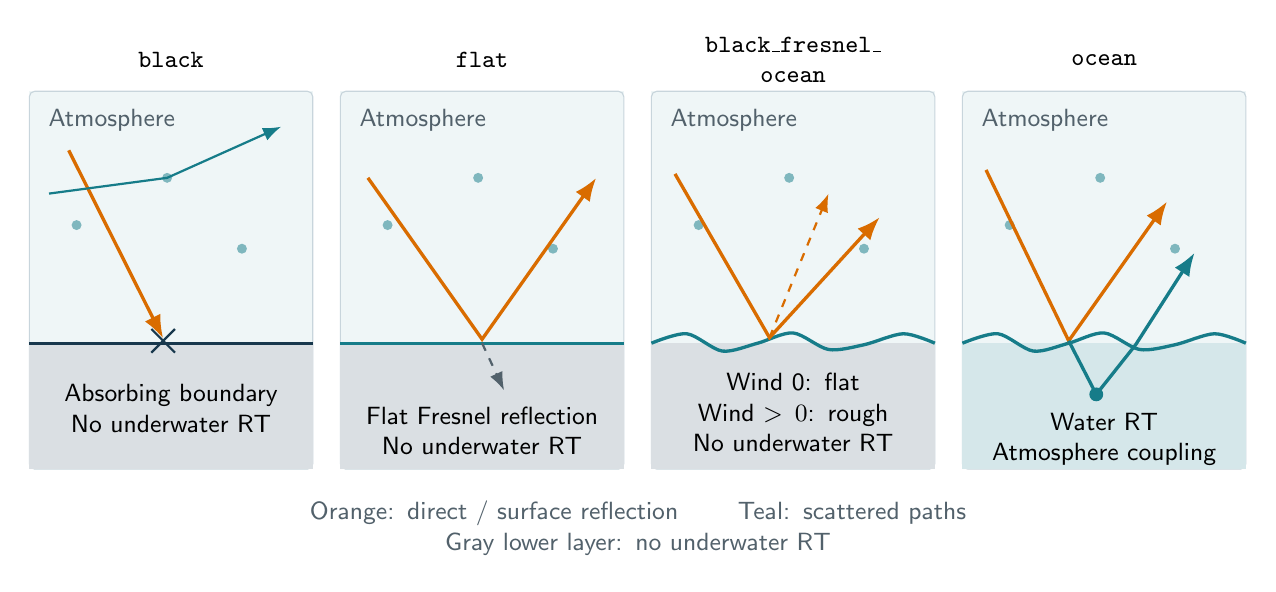
\begin{tikzpicture}[x=1cm,y=1cm,font=\sffamily\fontsize{9}{11}\selectfont,>=Latex]
\foreach \x in {0,3.95,7.9,11.85}{
  \fill[ocrtTeal!7] (\x,1.6) rectangle +(3.6,3.2);
  \draw[ocrtLine,rounded corners=2pt] (\x,0) rectangle +(3.6,4.8);
  \node[anchor=north west,text=ocrtGray] at (\x+0.12,4.7) {\FigLang{대기}{Atmosphere}};
  \foreach \px/\py in {0.6/3.1,1.75/3.7,2.7/2.8}{\fill[ocrtTeal!55] (\x+\px,\py) circle (1.8pt);}
}
\node[align=center,font=\sffamily\bfseries\fontsize{9}{11}\selectfont] at (1.8,5.2) {\texttt{black}};
\node[align=center,font=\sffamily\bfseries\fontsize{9}{11}\selectfont] at (5.75,5.2) {\texttt{flat}};
\node[align=center,font=\sffamily\bfseries\fontsize{9}{11}\selectfont] at (9.7,5.2) {\texttt{black\_fresnel\_}\vphantom{g}\\\texttt{ocean}};
\node[align=center,font=\sffamily\bfseries\fontsize{9}{11}\selectfont] at (13.65,5.2) {\texttt{ocean}};
% Absorbing lower boundary; atmospheric scattering remains active.
\fill[ocrtNavy!16] (0,0) rectangle (3.6,1.6);
\draw[ocrtNavy,very thick] (0,1.6)--(3.6,1.6);
\draw[->,orange!85!black,very thick] (0.5,4.05)--(1.7,1.66);
\draw[ocrtNavy,thick] (1.55,1.48)--(1.85,1.78) (1.55,1.78)--(1.85,1.48);
\draw[->,ocrtTeal,thick] (0.25,3.5)--(1.75,3.7)--(3.2,4.35);
\node[align=center,text width=3.15cm] at (1.8,0.77) {\FigLang{반사 없는 하부 경계\\수중 RT 없음}{Absorbing boundary\\No underwater RT}};
% Flat Fresnel, with absorption below.
\fill[ocrtNavy!16] (3.95,0) rectangle +(3.6,1.6);
\draw[ocrtTeal,very thick] (3.95,1.6)--+(3.6,0);
\draw[->,orange!85!black,very thick] (4.3,3.7)--(5.75,1.65)--(7.2,3.7);
\draw[->,ocrtGray,dashed,thick] (5.75,1.6)--(6.03,1.0);
\node[align=center,text width=3.15cm] at (5.75,0.49) {\FigLang{평면 Fresnel 반사\\수중 RT 없음}{Flat Fresnel reflection\\No underwater RT}};
% Rough Fresnel, with absorption below.
\fill[ocrtNavy!16] (7.9,0) rectangle +(3.6,1.6);
\draw[ocrtTeal,very thick] plot[smooth] coordinates {(7.9,1.6)(8.35,1.72)(8.8,1.5)(9.25,1.6)(9.7,1.73)(10.15,1.52)(10.6,1.58)(11.1,1.72)(11.5,1.6)};
\draw[->,orange!85!black,very thick] (8.2,3.75)--(9.4,1.67)--(10.8,3.2);
\draw[->,orange!85!black,thick,dashed] (9.4,1.67)--(10.15,3.5);
\node[align=center,text width=3.25cm] at (9.7,0.72) {\FigLang{풍속 0: 평면\\양수: 거친 해면\\수중 RT 없음}{Wind 0: flat\\Wind $>0$: rough\\No underwater RT}};
% Coupled atmosphere, rough surface, and water scattering.
\fill[ocrtTeal!18] (11.85,0) rectangle +(3.6,1.6);
\draw[ocrtTeal,very thick] plot[smooth] coordinates {(11.85,1.6)(12.3,1.72)(12.75,1.5)(13.2,1.6)(13.65,1.73)(14.1,1.52)(14.55,1.58)(15.05,1.72)(15.45,1.6)};
\draw[->,orange!85!black,very thick] (12.15,3.8)--(13.2,1.63)--(14.45,3.4);
\draw[->,ocrtTeal,very thick] (13.2,1.63)--(13.55,0.95)--(14.05,1.58)--(14.8,2.75);
\fill[ocrtTeal] (13.55,0.95) circle (2.5pt);
\node[align=center,text width=3.25cm] at (13.65,0.38) {\FigLang{수중 흡수·산란\\결합 RT}{Water RT\\Atmosphere coupling}};
\node[anchor=north,align=center,text width=15.1cm,text=ocrtGray] at (7.73,-0.28) {\FigLang{주황: 직달 입사·표면 반사 \qquad 청록: 산란을 거친 경로\\회색 하부: 수중 복사장 미계산}{Orange: direct / surface reflection \qquad Teal: scattered paths\\Gray lower layer: no underwater RT}};
\end{tikzpicture}
\caption{\FigLang{\texttt{--surface}는 하부 경계와 수중 계산의 범위를 선택한다. 거친 해면은 경사 분포를 개념적으로 그린 것으로 실제 파도를 공간적으로 추적하는 계산이 아니다. \texttt{ocean}만 수질/IOP를 이용해 수중 복사전달을 결합한다. 직달 glint의 출력 포함 여부는 다음 그림의 분리 규칙을 따른다.}{\texttt{--surface} selects the lower boundary and whether underwater RT is solved. The rough surface depicts a statistical slope distribution, not spatially resolved wave tracing. Only \texttt{ocean} couples underwater RT using water constituents/IOPs. Direct-glint inclusion follows the output separation rules in the next figure.}}
\label{fig:options-surfaces}
\end{figure}



{\TableFont
\begin{longtable}{@{}>{\raggedright\arraybackslash}p{\dimexpr 0.3000\linewidth-5.33pt\relax}>{\raggedright\arraybackslash}p{\dimexpr 0.2300\linewidth-5.33pt\relax}>{\raggedright\arraybackslash}p{\dimexpr 0.4700\linewidth-5.33pt\relax}@{}}
\toprule
\textbf{Option} & \textbf{Value / default} & \textbf{Description and conditions} \\
\midrule
\endfirsthead
\toprule
\textbf{Option} & \textbf{Value / default} & \textbf{Description and conditions} \\
\midrule
\endhead
\bottomrule
\endfoot
\texttt{-\allowbreak{}-\allowbreak{}sza DEG} & Degrees; required for normal runs; \texttt{0 \ensuremath{\leq} SZA < 90} & Zenith angle toward the Sun from the pixel. This is not an option for nighttime calculations. \\
\texttt{-\allowbreak{}-\allowbreak{}vza DEG} & Degrees; required for single geometry; \texttt{0 \ensuremath{\leq} VZA < 90} & Viewing zenith angle on the air side. Do not enter the underwater refracted angle directly. \\
\texttt{-\allowbreak{}-\allowbreak{}raa DEG} & Degrees; required for single geometry & OCRT relative azimuth angle. Normally enter \texttt{0 \ensuremath{\leq} RAA < 360}. \textbf{RAA=180\textdegree{} is the direct sunglint branch; 0\textdegree{} is the opposite principal-plane branch.} Do not copy RAA from another model or satellite product without conversion. \\
\texttt{-\allowbreak{}-\allowbreak{}wavelength NM} & nm; required for normal runs; \texttt{330 \ensuremath{\leq} \ensuremath{\lambda} \ensuremath{\leq} 1100} & Monochromatic calculation wavelength. External \texttt{.\allowbreak{}mie} files and LUTs must also support this wavelength. There is no option for extrapolation beyond the supported range. \\
\texttt{-\allowbreak{}-\allowbreak{}surface STR} & Required & Select one of the four surfaces below. \\
\texttt{-\allowbreak{}-\allowbreak{}wind-\allowbreak{}speed MS} & m s\textsuperscript{-}\textsuperscript{1}; nonnegative & Required for \texttt{ocean} and \texttt{black\_\allowbreak{}fresnel\_\allowbreak{}ocean}. Explicitly enter \texttt{0} for calm conditions. \\
\texttt{-\allowbreak{}-\allowbreak{}n-\allowbreak{}water X} & Dimensionless; default \texttt{1.\allowbreak{}34} & Real refractive index at the air--water interface. Use a physical seawater value (\texttt{>1}). This default does not automatically vary the interface index with temperature, salinity, or wavelength. \\
\texttt{-\allowbreak{}-\allowbreak{}decouple-\allowbreak{}sunglint} & Flag without a value; normally OFF & Separates and excludes the direct sunglint single-reflection term from non-ocean target results. It does not remove all surface reflection or atmosphere--surface interactions. The direct IOP path internally forces this flag ON. The default ocean TOA separates direct glint in a distinct composition path, so do not interpret OFF simply as inclusion (\hyperref[chap:05_output_formats]{output definitions}). \\
\texttt{-\allowbreak{}-\allowbreak{}pssa} & Flag without a value; default OFF & Enables the current implementation's spherical correction, \textbf{IPSS}. Angles refer to the ground pixel. Applies to atmospheric/black-ocean paths; it is unsupported for coupled \texttt{-\allowbreak{}-\allowbreak{}surface ocean} runs and produces an error. \\
\end{longtable}
}

Read the geometry/output interpretation chapter for RAA conversion equations, scattering angle, and polarization signs. In particular, calculating only \texttt{abs(sensor\_\allowbreak{}azimuth -\allowbreak{} solar\_\allowbreak{}azimuth)} and calling it OCRT RAA can reverse the glint direction.


{\TableFont
\begin{longtable}{@{}>{\raggedright\arraybackslash}p{\dimexpr 0.3400\linewidth-4.00pt\relax}>{\raggedright\arraybackslash}p{\dimexpr 0.6600\linewidth-4.00pt\relax}@{}}
\toprule
\textbf{\texttt{-\allowbreak{}-\allowbreak{}surface} value} & \textbf{Meaning} \\
\midrule
\endfirsthead
\toprule
\textbf{\texttt{-\allowbreak{}-\allowbreak{}surface} value} & \textbf{Meaning} \\
\midrule
\endhead
\bottomrule
\endfoot
\texttt{black} & Nonreflecting lower boundary. Used to calculate the atmospheric signal excluding water-surface reflection. \\
\texttt{flat} & Flat Fresnel boundary over a black ocean. Does not solve underwater scattering or a water-property model. \\
\texttt{black\_\allowbreak{}fresnel\_\allowbreak{}ocean} & Path with a black ocean beneath a Fresnel-reflecting sea surface. \texttt{-\allowbreak{}-\allowbreak{}wind-\allowbreak{}speed 0} gives a flat surface; positive wind gives a rough surface. Used for atmospheric and surface terms in ocean atmospheric correction. \\
\texttt{ocean} & Coupled atmosphere--sea-surface--underwater radiative transfer. Requires \texttt{-\allowbreak{}-\allowbreak{}water-\allowbreak{}model ocrt\textbackslash{}|ccrr\allowbreak{}\textbackslash{}|iop} and the corresponding water-property inputs. \\
\end{longtable}
}

\texttt{black-\allowbreak{}fresnel-\allowbreak{}ocean} is a current alias of \texttt{black\_\allowbreak{}fresnel\_\allowbreak{}ocean}. \texttt{coxmunk} is also recognized but is interpreted as \texttt{black\_\allowbreak{}fresnel\_\allowbreak{}ocean} with a deprecation warning. \texttt{lambert} produces an error because its boundary condition is not implemented.

\Needspace{7\baselineskip}
% Direct glint is attenuated but has no atmospheric scattering along its path.
\begin{figure}[H]
\centering
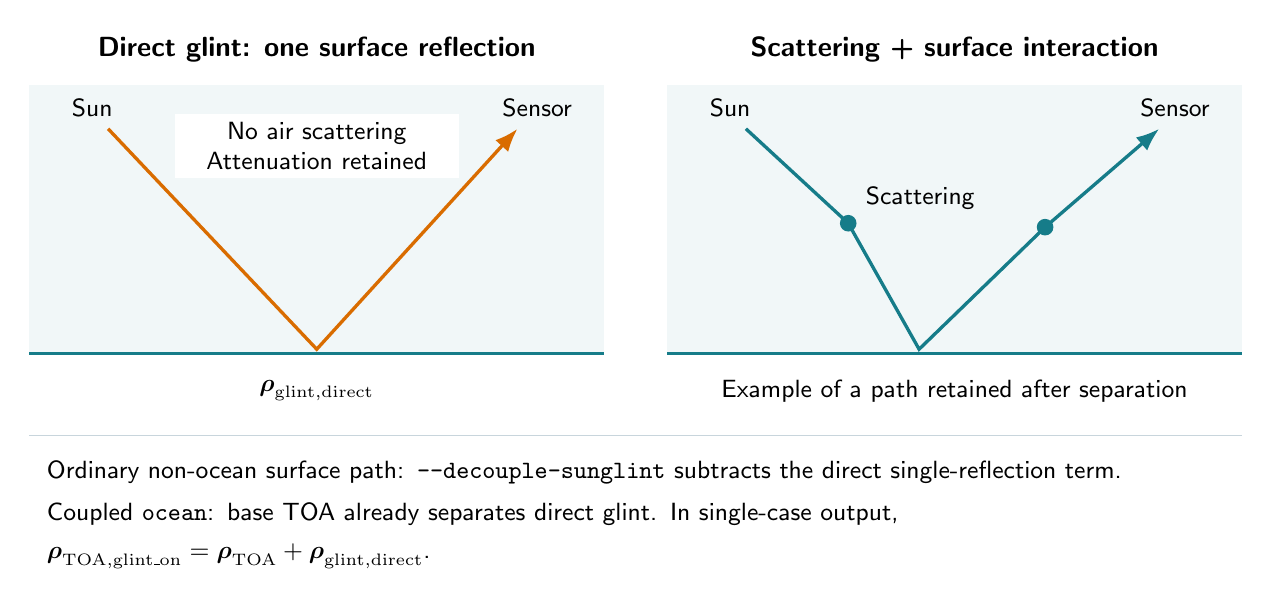
\begin{tikzpicture}[x=1cm,y=1cm,font=\sffamily\fontsize{9}{11}\selectfont,>=Latex]
\fill[ocrtTeal!6] (0,1) rectangle (7.3,4.4);
\fill[ocrtTeal!6] (8.1,1) rectangle (15.4,4.4);
\draw[ocrtTeal,very thick] (0,1)--(7.3,1) (8.1,1)--(15.4,1);
\node[anchor=south,align=center,font=\sffamily\bfseries\fontsize{10}{12}\selectfont] at (3.65,4.58) {\FigLang{직달 glint: 수면에서 한 번 반사}{Direct glint: one surface reflection}};
\node[anchor=south,align=center,font=\sffamily\bfseries\fontsize{10}{12}\selectfont] at (11.75,4.58) {\FigLang{산란 + 표면 상호작용}{Scattering + surface interaction}};
\node at (0.8,4.12) {\FigLang{태양}{Sun}};
\node at (6.45,4.12) {\FigLang{센서}{Sensor}};
\draw[->,orange!85!black,very thick] (1.0,3.85)--(3.65,1.05)--(6.2,3.85);
\node[align=center,text width=3.4cm,fill=white,inner sep=3pt] at (3.65,3.63) {\FigLang{대기 산란 0회\\대기 감쇠는 적용}{No air scattering\\Attenuation retained}};
\node[anchor=north,align=center,text width=7.1cm] at (3.65,0.78) {$\boldsymbol{\rho}_{\mathrm{glint,direct}}$};
\node at (8.9,4.12) {\FigLang{태양}{Sun}};
\node at (14.55,4.12) {\FigLang{센서}{Sensor}};
\draw[->,ocrtTeal,very thick] (9.1,3.85)--(10.4,2.65)--(11.3,1.05)--(12.9,2.6)--(14.35,3.85);
\fill[ocrtTeal] (10.4,2.65) circle (3pt);
\fill[ocrtTeal] (12.9,2.6) circle (3pt);
\node[anchor=south west] at (10.5,2.7) {\FigLang{산란}{Scattering}};
\node[anchor=north,align=center,text width=7.1cm] at (11.75,0.78) {\FigLang{분리 후에도 남는 경로의 예}{Example of a path retained after separation}};
\draw[ocrtLine] (0,-0.05)--(15.4,-0.05);
\node[anchor=north west,align=left,text width=15cm] at (0.1,-0.25) {\FigLang{일반 비해양 표면 경로: \texttt{--decouple-sunglint}가 직달 단일반사 항을 사후 제외한다.}{Ordinary non-ocean surface path: \texttt{--decouple-sunglint} subtracts the direct single-reflection term.}\\[4pt]
\FigLang{결합 \texttt{ocean}: 기본 TOA는 이미 직달 glint를 분리한다. 단일 결과에서}{Coupled \texttt{ocean}: base TOA already separates direct glint. In single-case output,}\\[3pt]
$\displaystyle \boldsymbol{\rho}_{\mathrm{TOA,glint\_on}}=\boldsymbol{\rho}_{\mathrm{TOA}}+\boldsymbol{\rho}_{\mathrm{glint,direct}}$.};
\end{tikzpicture}
\caption{\FigLang{\texttt{--decouple-sunglint}는 모든 표면 반사를 끄는 옵션이 아니다. 수면 반사와 대기 산란이 섞인 경로는 남는다. 해양 TOA의 기본 합성과 직접 IOP 경로의 강제 분리 때문에 단순히 플래그 OFF를 ``직달 glint 포함''으로 읽을 수 없다. 벡터 표기는 해당 I, Q, U 성분을 함께 뜻한다.}{\texttt{--decouple-sunglint} does not disable every surface reflection: paths involving both atmospheric scattering and surface reflection remain. The ocean TOA composition and forced separation in the direct-IOP path prevent a universal ``flag OFF means included'' rule. Bold reflectances denote the corresponding I, Q, and U components.}}
\label{fig:options-glint}
\end{figure}


\section{Rayleigh Atmosphere and Gas Absorption}
\label{sec:auto:03_options:3}
% Vertical profiles are conceptual normalized shapes, not AFGL measurements.
\begin{figure}[H]
\centering
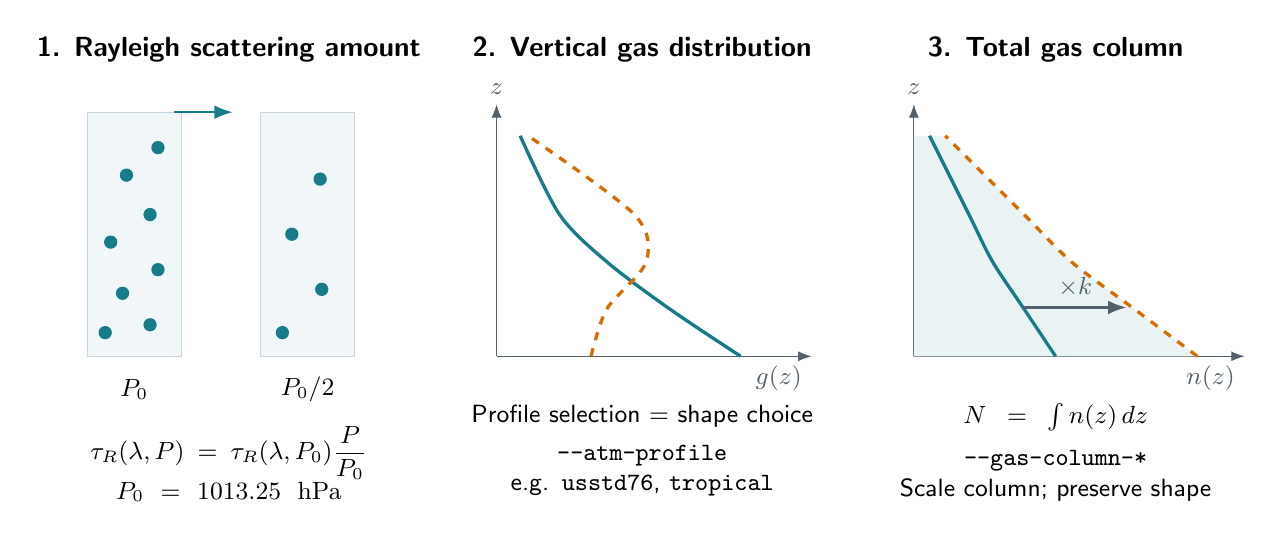
\begin{tikzpicture}[x=1cm,y=1cm,font=\sffamily\fontsize{9}{11}\selectfont,>=Latex]
\node[align=center,font=\sffamily\bfseries\fontsize{10}{12}\selectfont] at (2.4,5.7) {\FigLang{1. Rayleigh 산란의 크기}{1. Rayleigh scattering amount}};
\node[align=center,font=\sffamily\bfseries\fontsize{10}{12}\selectfont] at (7.65,5.7) {\FigLang{2. 기체의 수직 분포}{2. Vertical gas distribution}};
\node[align=center,font=\sffamily\bfseries\fontsize{10}{12}\selectfont] at (12.9,5.7) {\FigLang{3. 기체의 총량}{3. Total gas column}};
\foreach \x in {0.6,2.8}{\fill[ocrtTeal!6] (\x,1.8) rectangle +(1.2,3.1);\draw[ocrtLine] (\x,1.8) rectangle +(1.2,3.1);}
\foreach \px/\py in {0.83/2.1,1.4/2.2,1.05/2.6,1.5/2.9,0.9/3.25,1.4/3.6,1.1/4.1,1.5/4.45}{\fill[ocrtTeal] (\px,\py) circle (2.4pt);}
\foreach \px/\py in {3.08/2.1,3.58/2.65,3.2/3.35,3.56/4.05}{\fill[ocrtTeal] (\px,\py) circle (2.4pt);}
\node[align=center] at (1.2,1.38) {$P_0$};
\node[align=center] at (3.4,1.38) {$P_0/2$};
\draw[->,ocrtTeal,thick] (1.7,4.9)--(2.45,4.9);
\node[align=center,text width=4.6cm] at (2.4,0.43) {$\tau_R(\lambda,P)=\tau_R(\lambda,P_0)\dfrac{P}{P_0}$\\$P_0=1013.25\;\mathrm{hPa}$};
% Two alternative normalized shape sketches; equal column is merely illustrative.
\draw[->,ocrtGray] (5.8,1.8)--(9.8,1.8) node[below left] {$g(z)$};
\draw[->,ocrtGray] (5.8,1.8)--(5.8,5.0) node[above] {$z$};
\draw[ocrtTeal,very thick] plot[smooth] coordinates {(8.9,1.8)(8.0,2.4)(7.2,3.0)(6.6,3.6)(6.1,4.6)};
\draw[orange!85!black,very thick,dashed] plot[smooth] coordinates {(7.0,1.8)(7.2,2.4)(7.7,3.0)(7.55,3.6)(6.2,4.6)};
\node[align=center,text width=4.75cm] at (7.65,1.04) {\FigLang{프로파일 선택 = 형태 선택}{Profile selection = shape choice}};
\node[align=center,text width=4.7cm] at (7.65,0.35) {\texttt{--atm-profile}\\\FigLang{예: \texttt{usstd76}, \texttt{tropical}}{e.g. \texttt{usstd76}, \texttt{tropical}}};
% Scaling the same shape preserves height-dependent relative distribution.
\draw[->,ocrtGray] (11.1,1.8)--(15.3,1.8) node[below left] {$n(z)$};
\draw[->,ocrtGray] (11.1,1.8)--(11.1,5.0) node[above] {$z$};
\fill[ocrtTeal!9] (11.1,1.8)--(14.7,1.8)--(13.9,2.4)--(13.1,3.0)--(12.5,3.6)--(11.5,4.6)--(11.1,4.6)--cycle;
\draw[ocrtTeal,very thick] plot[smooth] coordinates {(12.9,1.8)(12.5,2.4)(12.1,3.0)(11.8,3.6)(11.3,4.6)};
\draw[orange!85!black,very thick,dashed] plot[smooth] coordinates {(14.7,1.8)(13.9,2.4)(13.1,3.0)(12.5,3.6)(11.5,4.6)};
\draw[->,ocrtGray,thick] (12.5,2.42)--(13.8,2.42) node[midway,above] {$\times k$};
\node[align=center,text width=4.8cm] at (12.9,1.02) {$N=\int n(z)\,dz$};
\node[align=center,text width=4.85cm] at (12.9,0.28) {\texttt{--gas-column-*}\\\FigLang{형태를 보존하며 총량 조절}{Scale column; preserve shape}};
\end{tikzpicture}
\caption{\FigLang{\texttt{--pressure}는 Rayleigh 광학두께를, \texttt{--atm-profile}은 기체흡수 프로파일을, \texttt{--gas-column-*}는 각 기체의 총량을 조절한다. 그림의 점·곡선은 개념도이며 실제 AFGL 값이 아니다. 압력 0만으로 기체흡수는 꺼지지 않는다. 컬럼 단위는 H$_2$O: g cm$^{-2}$, O$_3$/NO$_2$: DU, O$_2$/CO$_2$/CH$_4$: molecules cm$^{-2}$다.}{\texttt{--pressure} scales Rayleigh optical depth, \texttt{--atm-profile} selects the gas-absorption profile, and \texttt{--gas-column-*} sets each gas column. Dots and curves are conceptual, not AFGL data. Pressure 0 does not disable gas absorption. Column units are g cm$^{-2}$ for H$_2$O, DU for O$_3$/NO$_2$, and molecules cm$^{-2}$ for O$_2$/CO$_2$/CH$_4$.}}
\label{fig:options-gas}
\end{figure}



{\TableFont
\begin{longtable}{@{}>{\raggedright\arraybackslash}p{\dimexpr 0.3000\linewidth-5.33pt\relax}>{\raggedright\arraybackslash}p{\dimexpr 0.2300\linewidth-5.33pt\relax}>{\raggedright\arraybackslash}p{\dimexpr 0.4700\linewidth-5.33pt\relax}@{}}
\toprule
\textbf{Option} & \textbf{Value / default} & \textbf{Description} \\
\midrule
\endfirsthead
\toprule
\textbf{Option} & \textbf{Value / default} & \textbf{Description} \\
\midrule
\endhead
\bottomrule
\endfoot
\texttt{-\allowbreak{}-\allowbreak{}pressure P} & hPa; default \texttt{1013.\allowbreak{}25}; \texttt{P \ensuremath{\geq} 0} & Scales Rayleigh optical thickness by \texttt{P/\allowbreak{}1013.\allowbreak{}25} relative to standard pressure. \texttt{0} removes Rayleigh scattering. Independent of gas absorption and aerosols. \\
\texttt{-\allowbreak{}-\allowbreak{}surface-\allowbreak{}pressure P} & Same as above & Alias of \texttt{-\allowbreak{}-\allowbreak{}pressure}. \\
\texttt{-\allowbreak{}-\allowbreak{}no-\allowbreak{}rayleigh} & Flag without a value & Compatibility option retained in the current parser. Sets pressure to \texttt{0}. Use \texttt{-\allowbreak{}-\allowbreak{}pressure 0} in new commands. \\
\texttt{-\allowbreak{}-\allowbreak{}rayleigh on\textbackslash{}|off\allowbreak{}} & Pressure-based by default & \texttt{off} sets pressure to \texttt{0}. \texttt{on} restores \texttt{1013.\allowbreak{}25} if the current pressure is \texttt{\ensuremath{\leq}0}, retaining an existing positive pressure. A later \texttt{-\allowbreak{}-\allowbreak{}pressure} takes precedence. \\
\texttt{-\allowbreak{}-\allowbreak{}atm-\allowbreak{}profile STR} & Default \texttt{usstd76} & AFGL vertical profile for gas absorption: \texttt{usstd76}, \texttt{tropical}, \texttt{mlsumm}, \texttt{mlwint}, \texttt{sasumm}, \texttt{sawint}, \texttt{userdef}. \\
\texttt{-\allowbreak{}-\allowbreak{}gas-\allowbreak{}profile STR} & Same as above & Alias of \texttt{-\allowbreak{}-\allowbreak{}atm-\allowbreak{}profile}. \\
\texttt{-\allowbreak{}-\allowbreak{}gas-\allowbreak{}column-\allowbreak{}h2o G} & g cm\textsuperscript{-}\textsuperscript{2}; default AFGL integral & Total water vapor. \texttt{G \ensuremath{\geq} 0}. Converted to a water-molecule column, then scaled to the total while preserving the selected vertical profile's shape. \\
\texttt{-\allowbreak{}-\allowbreak{}pwv-\allowbreak{}g-\allowbreak{}cm G} & Same as above & Alias of \texttt{-\allowbreak{}-\allowbreak{}gas-\allowbreak{}column-\allowbreak{}h2o}. \\
\texttt{-\allowbreak{}-\allowbreak{}gas-\allowbreak{}column-\allowbreak{}o3 DU} & DU; default AFGL integral & Total ozone. \texttt{DU \ensuremath{\geq} 0}. \texttt{1 DU =\allowbreak{} 2.\allowbreak{}6868\ensuremath{\times}10\textsuperscript{1}\textsuperscript{6} molecu\allowbreak{}les cm\textsuperscript{-}\textsuperscript{2}}. \\
\texttt{-\allowbreak{}-\allowbreak{}gas-\allowbreak{}column-\allowbreak{}no2 DU} & DU; default AFGL integral & Total nitrogen dioxide. Uses the same DU conversion as O\textsubscript{3}. \\
\texttt{-\allowbreak{}-\allowbreak{}gas-\allowbreak{}column-\allowbreak{}o2 N} & \textbf{molecules cm\textsuperscript{-}\textsuperscript{2}}; default AFGL integral & Oxygen molecule column. Nonnegative. \\
\texttt{-\allowbreak{}-\allowbreak{}gas-\allowbreak{}column-\allowbreak{}co2 N} & \textbf{molecules cm\textsuperscript{-}\textsuperscript{2}}; default AFGL integral & Carbon dioxide molecule column. Do not enter a ppm value directly. \\
\texttt{-\allowbreak{}-\allowbreak{}gas-\allowbreak{}column-\allowbreak{}ch4 N} & \textbf{molecules cm\textsuperscript{-}\textsuperscript{2}}; default AFGL integral & Methane molecule column. Nonnegative. \\
\end{longtable}
}

\textbf{Unit correction:} The \texttt{mol/\allowbreak{}cm\textsuperscript{2}} notation in older help and standard-error logs means \textbf{molecules/cm\textsuperscript{2}}, not moles. The actual H\textsubscript{2}O conversion is \texttt{G \ensuremath{\times} 6.\allowbreak{}02214076e23 /\allowbreak{} 18.\allowbreak{}01528}. Entering mol cm\textsuperscript{-}\textsuperscript{2} for O\textsubscript{2}, CO\textsubscript{2}, or CH\textsubscript{4} produces an input error by a factor of Avogadro's number.

Gas absorption is enabled by default in single/grid runs. For a pure Rayleigh reference calculation, explicitly set all six values below.


\begin{ManualCode}
--gas-column-h2o 0 --gas-column-o3 0 --gas-column-no2 0 --gas-column-o2 0 --gas-column-co2 0 --gas-column-ch4 0
\end{ManualCode}

Each gas's default column depends on the profile and distributed data. Record the actual log's \texttt{column=\allowbreak{}} and \texttt{overridden} indicators. Negative values may be treated internally as unspecified-value markers, so do not use them to disable absorption. Put a user profile in \texttt{inputs/\allowbreak{}afgl\_\allowbreak{}atm/\allowbreak{}afgl\_\allowbreak{}userdef.\allowbreak{}dat} and select it with \texttt{-\allowbreak{}-\allowbreak{}atm-\allowbreak{}profile userdef}. \texttt{-\allowbreak{}-\allowbreak{}atm-\allowbreak{}profile} selects a gas profile; it does not select one of seven models for the Rayleigh molecular atmosphere itself.

\section{Aerosols}
\label{sec:auto:03_options:4}
\begin{figure}[H]
\centering
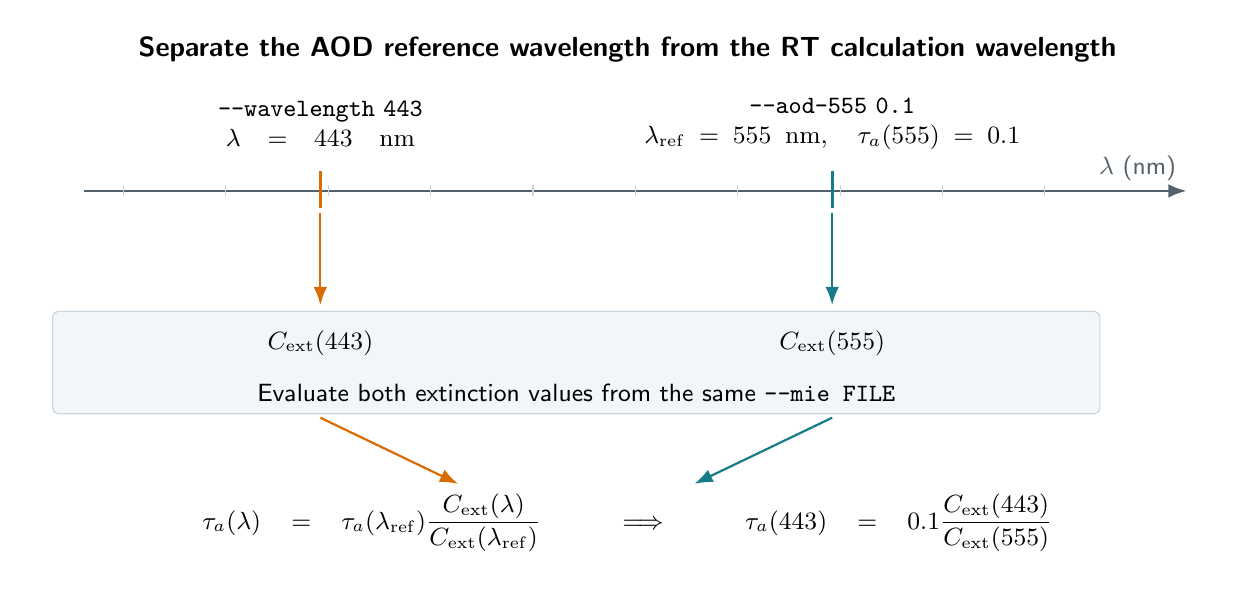
\begin{tikzpicture}[x=1cm,y=1cm,font=\sffamily\fontsize{9}{11}\selectfont,>=Latex]
\node[align=center,font=\sffamily\bfseries\fontsize{10}{12}\selectfont] at (7.7,5.3) {\FigLang{AOD를 지정하는 파장과 복사전달 계산 파장을 구분한다}{Separate the AOD reference wavelength from the RT calculation wavelength}};
\draw[->,ocrtGray,thick] (0.8,3.5)--(14.8,3.5) node[above left] {$\lambda$ (nm)};
\foreach \x in {1.3,2.6,3.9,5.2,6.5,7.8,9.1,10.4,11.7,13.0}{\draw[ocrtLine] (\x,3.43)--(\x,3.57);}
\draw[orange!85!black,very thick] (3.8,3.28)--(3.8,3.75);
\draw[ocrtTeal,very thick] (10.3,3.28)--(10.3,3.75);
\node[align=center,text width=6cm] at (3.8,4.35) {\texttt{--wavelength 443}\\$\lambda=443\;\mathrm{nm}$};
\node[align=center,text width=6cm] at (10.3,4.35) {\texttt{--aod-555 0.1}\\$\lambda_{\rm ref}=555\;\mathrm{nm},\quad \tau_a(555)=0.1$};
\draw[->,orange!85!black,thick] (3.8,3.22)--(3.8,2.05);
\draw[->,ocrtTeal,thick] (10.3,3.22)--(10.3,2.05);
\node[draw=ocrtLine,fill=ocrtTeal!6,rounded corners=2pt,minimum width=13.3cm,minimum height=1.3cm] at (7.05,1.32) {};
\node at (3.8,1.57) {$C_{\rm ext}(443)$};
\node at (10.3,1.57) {$C_{\rm ext}(555)$};
\node[align=center] at (7.05,0.94) {\FigLang{같은 \texttt{--mie FILE}에서 두 파장의 소광값을 평가}{Evaluate both extinction values from the same \texttt{--mie FILE}}};
\draw[->,orange!85!black,thick] (3.8,0.62)--(5.55,-0.22);
\draw[->,ocrtTeal,thick] (10.3,0.62)--(8.55,-0.22);
\node[align=center,text width=15cm] at (7.7,-0.72) {$\displaystyle \tau_a(\lambda)=\tau_a(\lambda_{\rm ref})\frac{C_{\rm ext}(\lambda)}{C_{\rm ext}(\lambda_{\rm ref})}\qquad\Longrightarrow\qquad \tau_a(443)=0.1\frac{C_{\rm ext}(443)}{C_{\rm ext}(555)}$};
\end{tikzpicture}
\caption{\FigLang{\texttt{--aod-555}, \texttt{--aod-865}, 또는 \texttt{--aod}와 \texttt{--aod-ref-wavelength}는 기준 AOD를 지정한다. \texttt{--wavelength}는 실제 계산 파장이다. 그림은 두 입력의 역할을 보여 주는 개념 축이며 수치 간격은 축척이 아니다. 파장별 AOD 비율은 사용한 Mie 파일에서 계산하므로 443 nm에서도 AOD가 자동으로 0.1이라고 가정하지 않는다.}{\texttt{--aod-555}, \texttt{--aod-865}, or \texttt{--aod} with \texttt{--aod-ref-wavelength} sets reference AOD; \texttt{--wavelength} sets the calculation wavelength. The axis distinguishes their roles and is not to scale. The Mie file determines the spectral extinction ratio, so the AOD at 443 nm is not automatically 0.1.}}
\label{fig:options-aod}
\end{figure}



{\TableFont
\begin{longtable}{@{}>{\raggedright\arraybackslash}p{\dimexpr 0.3000\linewidth-5.33pt\relax}>{\raggedright\arraybackslash}p{\dimexpr 0.2300\linewidth-5.33pt\relax}>{\raggedright\arraybackslash}p{\dimexpr 0.4700\linewidth-5.33pt\relax}@{}}
\toprule
\textbf{Option} & \textbf{Value / default} & \textbf{Description and conditions} \\
\midrule
\endfirsthead
\toprule
\textbf{Option} & \textbf{Value / default} & \textbf{Description and conditions} \\
\midrule
\endhead
\bottomrule
\endfoot
\texttt{-\allowbreak{}-\allowbreak{}mie FILE} & Aerosol \texttt{.\allowbreak{}mie}; none by default & Required if \texttt{AOD>0}. Its purpose differs from \texttt{-\allowbreak{}-\allowbreak{}iop-\allowbreak{}mie-\allowbreak{}phase}, the underwater particle phase-function file. \\
\texttt{-\allowbreak{}-\allowbreak{}aod-\allowbreak{}555 X} & Dimensionless; default \texttt{0}; \texttt{X \ensuremath{\geq} 0} & AOD referenced to 555 nm. AOD at the calculation wavelength is converted using the \texttt{.\allowbreak{}mie} extinction-coefficient ratio. \\
\texttt{-\allowbreak{}-\allowbreak{}aod-\allowbreak{}865 X} & Dimensionless & AOD referenced to 865 nm. \\
\texttt{-\allowbreak{}-\allowbreak{}aod X} & Dimensionless; default \texttt{0} & Compatibility input. AOD referenced to \texttt{-\allowbreak{}-\allowbreak{}aod-\allowbreak{}ref-\allowbreak{}wavelength}, not AOD at the current calculation wavelength. \\
\texttt{-\allowbreak{}-\allowbreak{}aod-\allowbreak{}ref-\allowbreak{}wavelength NM} & nm; default \texttt{555} & Reference wavelength for \texttt{-\allowbreak{}-\allowbreak{}aod}. The aerosol file must support both this reference wavelength and the calculation wavelength. \\
\texttt{-\allowbreak{}-\allowbreak{}aer-\allowbreak{}h-\allowbreak{}km H} & km; default \texttt{2.\allowbreak{}0}; \texttt{H>0} & Scale height of the aerosol vertical distribution \texttt{exp(-\allowbreak{}z/\allowbreak{}H)}. The current CLI checks positivity but implements no ADVANCED gate, unlike the older help's “advanced only” description. \\
\texttt{-\allowbreak{}-\allowbreak{}aer-\allowbreak{}l-\allowbreak{}max L} & Integer \texttt{L\ensuremath{\geq}2}; default \texttt{80} for active aerosols & Maximum order of aerosol phase moments. Requires \texttt{OCRT\_\allowbreak{}ADVANCED=\allowbreak{}1} when different from the default. \\
\end{longtable}
}

Use only one AOD input form to avoid confusing reference wavelengths. Combining multiple \texttt{-\allowbreak{}-\allowbreak{}aod-\allowbreak{}*} options changes the AOD value and reference wavelength according to parsing order. For example, \texttt{-\allowbreak{}-\allowbreak{}aod-\allowbreak{}555 0.\allowbreak{}1 -\allowbreak{}-\allowbreak{}aod-\allowbreak{}ref-\allowbreak{}wavelength 865} ultimately means AOD 0.1 at 865 nm.

In non-batch runs with AOD 0, you cannot also specify \texttt{-\allowbreak{}-\allowbreak{}mie}, \texttt{-\allowbreak{}-\allowbreak{}aer-\allowbreak{}h-\allowbreak{}km}, \texttt{-\allowbreak{}-\allowbreak{}aer-\allowbreak{}l-\allowbreak{}max}, or aerosol truncation options. For AOD>0, the default choices are the value kernel, physical-angle log10-linear forward-peak truncation, \texttt{L=\allowbreak{}80}, atmospheric Fourier \texttt{m=\allowbreak{}16}, and 400 atmospheric layers. Distinguish this default aerosol truncation from the underwater particle FR631 policy of truncation OFF by default.

\texttt{T50}, \texttt{C50}, and \texttt{M80C} are the officially validated subset identified by the code. If a filename contains \texttt{M50C}, the current parser requires \texttt{OCRT\_\allowbreak{}DEBUG=\allowbreak{}1} and issues a diagnostic-use warning. See the \href{https://github.com/brtnt/OCRT/blob/54861c68e35ec5aaa3938fad53e93dc2dfa7eb1d/code/OCRT_C/inputs/deprecated/DEPRECATED_M50C.md}{M50C record} for the model's provenance issue.

\section{Common Underwater Model Inputs}
\label{sec:auto:03_options:5}
\begin{figure}[H]
\centering
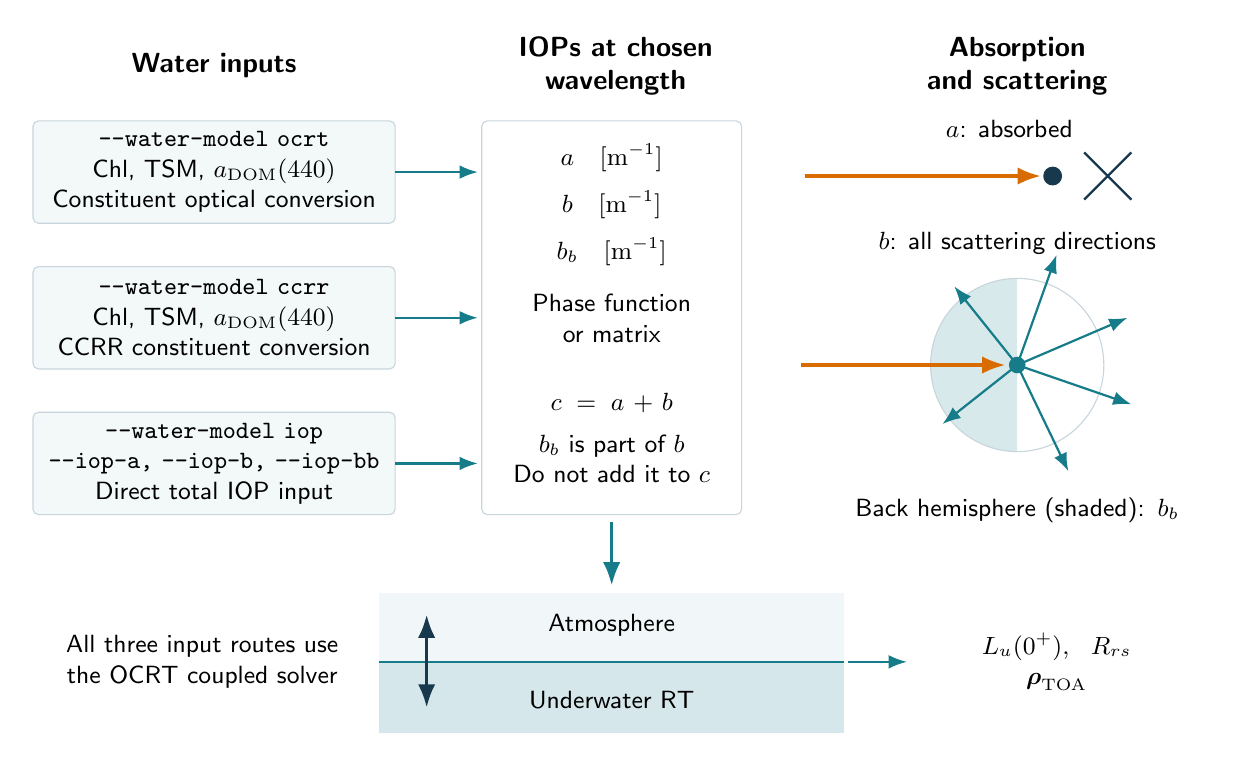
\begin{tikzpicture}[x=1cm,y=1cm,font=\sffamily\fontsize{9}{11}\selectfont,>=Latex]
\node[align=center,text width=4.5cm,font=\sffamily\bfseries\fontsize{10}{12}\selectfont] at (2.5,7.45) {\FigLang{수질 입력}{Water inputs}};
\node[align=center,text width=4.5cm,font=\sffamily\bfseries\fontsize{10}{12}\selectfont] at (7.6,7.45) {\FigLang{선택한 파장의 IOP}{IOPs at chosen\\wavelength}};
\node[align=center,text width=4.5cm,font=\sffamily\bfseries\fontsize{10}{12}\selectfont] at (12.7,7.45) {\FigLang{흡수와 산란의 의미}{Absorption\\and scattering}};
\foreach \y in {6.1,4.25,2.4}{\draw[ocrtLine,rounded corners=2pt,fill=ocrtTeal!5] (0.2,\y-0.65) rectangle (4.8,\y+0.65);}
\node[align=center,text width=4.3cm] at (2.5,6.1) {\texttt{--water-model ocrt}\\Chl, TSM, $a_{\rm DOM}(440)$\\\FigLang{성분별 물성으로 변환}{Constituent optical conversion}};
\node[align=center,text width=4.3cm] at (2.5,4.25) {\texttt{--water-model ccrr}\\Chl, TSM, $a_{\rm DOM}(440)$\\\FigLang{CCRR 구성성분 변환}{CCRR constituent conversion}};
\node[align=center,text width=4.3cm] at (2.5,2.4) {\texttt{--water-model iop}\\\texttt{--iop-a, --iop-b, --iop-bb}\\\FigLang{총 IOP를 직접 입력}{Direct total IOP input}};
\draw[ocrtLine,rounded corners=2pt,fill=white] (5.9,1.75) rectangle (9.2,6.75);
\foreach \y in {6.1,4.25,2.4}{\draw[->,ocrtTeal,thick] (4.8,\y)--(5.85,\y);}
\node[align=center,text width=3.1cm] at (7.55,5.2) {$a\quad[\mathrm{m}^{-1}]$\\[6pt]$b\quad[\mathrm{m}^{-1}]$\\[6pt]$b_b\quad[\mathrm{m}^{-1}]$\\[8pt]\FigLang{위상함수 / 행렬}{Phase function\\or matrix}};
\node[align=center,text width=2.95cm] at (7.55,2.72) {$c=a+b$\\[4pt]\FigLang{$b_b$는 $b$의 일부\\추가 소광항이 아님}{$b_b$ is part of $b$\\Do not add it to $c$}};
% Absorption terminates a ray.
\draw[->,orange!85!black,very thick] (10.0,6.05)--(13.0,6.05);
\fill[ocrtNavy] (13.15,6.05) circle (3.4pt);
\draw[ocrtNavy,thick] (13.55,5.75)--(14.15,6.35) (13.55,6.35)--(14.15,5.75);
\node[align=center] at (12.6,6.65) {$a$: \FigLang{흡수되어 소멸}{absorbed}};
% Scattering angular redistribution; back hemisphere is a subset.
\fill[ocrtTeal!17] (12.7,3.65)--(12.7,4.75) arc[start angle=90,end angle=270,radius=1.1]--cycle;
\draw[ocrtLine] (12.7,3.65) circle (1.1);
\draw[->,orange!85!black,very thick] (9.95,3.65)--(12.55,3.65);
\foreach \dx/\dy in {1.4/0.6,1.45/-0.5,0.5/1.4,0.65/-1.35,-0.8/1.0,-0.95/-0.75}{\draw[->,ocrtTeal,thick] (12.7,3.65)--+(\dx,\dy);}
\fill[ocrtTeal] (12.7,3.65) circle (3pt);
\node[align=center] at (12.7,5.2) {$b$: \FigLang{모든 산란 방향}{all scattering directions}};
\node[align=center,text width=4.9cm] at (12.7,1.8) {\FigLang{색칠한 뒤쪽 반구의 산란이 $b_b$}{Back hemisphere (shaded): $b_b$}};
\draw[->,ocrtTeal,very thick] (7.55,1.65)--(7.55,0.85);
% A physical stack, not a fourth alternative water model.
\fill[ocrtTeal!6] (4.6,-0.12) rectangle (10.5,0.75);
\fill[ocrtTeal!18] (4.6,-1.02) rectangle (10.5,-0.12);
\draw[ocrtTeal,thick] (4.6,-0.12)--(10.5,-0.12);
\node at (7.55,0.35) {\FigLang{대기}{Atmosphere}};
\node at (7.55,-0.6) {\FigLang{수중 복사전달}{Underwater RT}};
\draw[<->,ocrtNavy,very thick] (5.2,0.48)--(5.2,-0.7);
\node[align=center,text width=3.8cm] at (2.35,-0.12) {\FigLang{세 입력 경로 모두\\OCRT 결합 해석기 사용}{All three input routes use\\the OCRT coupled solver}};
\draw[->,ocrtTeal,thick] (10.55,-0.12)--(11.3,-0.12);
\node[align=center,text width=3.7cm] at (13.2,-0.12) {$L_u(0^+),\; R_{rs}$\\$\boldsymbol{\rho}_{\rm TOA}$};
\end{tikzpicture}
\caption{\FigLang{\texttt{--water-model}은 수질에서 광학 입력을 만드는 경로를 선택한다. OCRT/CCRR는 구성성분을 변환하고 IOP 모드는 순수 해수 기여까지 포함한 총 $a,b,b_b$를 직접 받는다. $b_b$는 후방 산란 부분이므로 소광계수는 $a+b$이며 $a+b+b_b$가 아니다. 위상함수는 산란 에너지가 각 방향으로 분배되는 모양을 정한다.}{\texttt{--water-model} selects the route from water properties to optical inputs. OCRT/CCRR convert constituents; IOP mode receives total $a,b,b_b$, already including pure seawater. Backscattering is a subset of scattering, so extinction is $a+b$, not $a+b+b_b$. The phase function describes how scattered energy is distributed over direction.}}
\label{fig:options-water}
\end{figure}



{\TableFont
\begin{longtable}{@{}>{\raggedright\arraybackslash}p{\dimexpr 0.3000\linewidth-5.33pt\relax}>{\raggedright\arraybackslash}p{\dimexpr 0.2300\linewidth-5.33pt\relax}>{\raggedright\arraybackslash}p{\dimexpr 0.4700\linewidth-5.33pt\relax}@{}}
\toprule
\textbf{Option} & \textbf{Value / default} & \textbf{Description} \\
\midrule
\endfirsthead
\toprule
\textbf{Option} & \textbf{Value / default} & \textbf{Description} \\
\midrule
\endhead
\bottomrule
\endfoot
\texttt{-\allowbreak{}-\allowbreak{}water-\allowbreak{}model M} & \texttt{ocrt}, \texttt{ccrr}, \texttt{iop} & Required exactly once with \texttt{-\allowbreak{}-\allowbreak{}surface ocean}. Cannot be used with another surface. \\
\texttt{-\allowbreak{}-\allowbreak{}water-\allowbreak{}temperature C} & \textdegree{}C; default \texttt{20} & Temperature correction input for pure-seawater IOPs. Separate from the interface refractive index \texttt{-\allowbreak{}-\allowbreak{}n-\allowbreak{}water}. \\
\texttt{-\allowbreak{}-\allowbreak{}water-\allowbreak{}salinity G} & g kg\textsuperscript{-}\textsuperscript{1}; default \texttt{38.\allowbreak{}4} & Salinity input for pure-seawater IOPs. Do not use negative values. \\
\end{longtable}
}

The CLI does not block every extrapolation range for temperature and salinity. Assess the range used in an experiment together with the sources and correction equations of the distributed pure-seawater data. All three models allow separate settings for atmospheric pressure, gas absorption, wind speed, and aerosols. For underwater-only calculations, use \texttt{-\allowbreak{}-\allowbreak{}pressure 0}, AOD 0, and all six gas columns set to 0 together.

\subsection{OCRT Constituent Model}
\label{sec:auto:03_options:5.1}

{\TableFont
\begin{longtable}{@{}>{\raggedright\arraybackslash}p{\dimexpr 0.3000\linewidth-5.33pt\relax}>{\raggedright\arraybackslash}p{\dimexpr 0.2300\linewidth-5.33pt\relax}>{\raggedright\arraybackslash}p{\dimexpr 0.4700\linewidth-5.33pt\relax}@{}}
\toprule
\textbf{Option} & \textbf{Value / default} & \textbf{Description and conditions} \\
\midrule
\endfirsthead
\toprule
\textbf{Option} & \textbf{Value / default} & \textbf{Description and conditions} \\
\midrule
\endhead
\bottomrule
\endfoot
\texttt{-\allowbreak{}-\allowbreak{}ocrt-\allowbreak{}chl X} & mg m\textsuperscript{-}\textsuperscript{3}; required; \texttt{X\ensuremath{\geq}0} & Chlorophyll-a concentration. The current production path uses phytoplankton absorption and detritus scattering; EAP species-specific scattering is inactive. \\
\texttt{-\allowbreak{}-\allowbreak{}ocrt-\allowbreak{}tsm X} & g m\textsuperscript{-}\textsuperscript{3}; required; \texttt{X\ensuremath{\geq}0} & Dry mass concentration of inorganic suspended matter. Distinguish this from general total suspended matter comprising all underwater constituents. \\
\texttt{-\allowbreak{}-\allowbreak{}ocrt-\allowbreak{}adom440 X} & m\textsuperscript{-}\textsuperscript{1}; required; \texttt{X\ensuremath{\geq}0} & Dissolved organic matter absorption coefficient at 440 nm. \\
\texttt{-\allowbreak{}-\allowbreak{}ocrt-\allowbreak{}adom-\allowbreak{}slope X} & nm\textsuperscript{-}\textsuperscript{1}; default \texttt{0.\allowbreak{}014}; \texttt{X>0} & \texttt{aDOM(\ensuremath{\lambda})=\allowbreak{}aDOM(440) exp[-\allowbreak{}X(\ensuremath{\lambda}-440)]}. \\
\texttt{-\allowbreak{}-\allowbreak{}ocrt-\allowbreak{}tsm-\allowbreak{}species N} & Default \texttt{red\_\allowbreak{}clay} & \texttt{red\_\allowbreak{}clay}, \texttt{brown\_\allowbreak{}earth}, \texttt{yellow\_\allowbreak{}clay}, \texttt{calcareous\_\allowbreak{}sand}. Explicit use requires \texttt{-\allowbreak{}-\allowbreak{}ocrt-\allowbreak{}tsm>0}. \\
\texttt{-\allowbreak{}-\allowbreak{}ocrt-\allowbreak{}detritus-\allowbreak{}a440 X} & m\textsuperscript{-}\textsuperscript{1}; default \texttt{0}; \texttt{X\ensuremath{\geq}0} & Organic detritus absorption input at 440 nm. Explicit use requires \texttt{-\allowbreak{}-\allowbreak{}ocrt-\allowbreak{}chl>0}. This is not an interface for independently enabling detritus at Chl=0. \textbf{0 means detritus absorption of 0; it does not also disable the detritus scattering derived from Chl.} \\
\texttt{-\allowbreak{}-\allowbreak{}ocrt-\allowbreak{}detritus-\allowbreak{}slope X} & nm\textsuperscript{-}\textsuperscript{1}; default \texttt{0.\allowbreak{}0109}; \texttt{X>0} & Exponential slope of the detritus absorption spectrum. Explicit use requires \texttt{-\allowbreak{}-\allowbreak{}ocrt-\allowbreak{}chl>0}. Positive values outside the source range \texttt{[0.\allowbreak{}0024,\allowbreak{}0.\allowbreak{}0170]} produce a warning and proceed. \\
\texttt{-\allowbreak{}-\allowbreak{}ocrt-\allowbreak{}phyto-\allowbreak{}group G} & Unavailable in current production runs & The parser recognizes \texttt{pico}, \texttt{nano}, \texttt{micro}, and canonical \texttt{eap\_\allowbreak{}*} species names, but exits with an unsupported-feature error for Chl>0. Chl=0 also fails a dependency check. Therefore, omit this option currently. \\
\end{longtable}
}

When \texttt{Chl=\allowbreak{}TSM=\allowbreak{}aDOM440=\allowbreak{}0}, both OCRT and CCRR descend to the same native pure-seawater path. All three values must be \textbf{explicitly specified even when 0}. Duplicate specifications of Chl, TSM, aDOM440, or aDOM slope are errors.

\subsection{CCRR Constituent Adapter}
\label{sec:auto:03_options:5.2}

{\TableFont
\begin{longtable}{@{}>{\raggedright\arraybackslash}p{\dimexpr 0.3000\linewidth-5.33pt\relax}>{\raggedright\arraybackslash}p{\dimexpr 0.2300\linewidth-5.33pt\relax}>{\raggedright\arraybackslash}p{\dimexpr 0.4700\linewidth-5.33pt\relax}@{}}
\toprule
\textbf{Option} & \textbf{Value / default} & \textbf{Description and conditions} \\
\midrule
\endfirsthead
\toprule
\textbf{Option} & \textbf{Value / default} & \textbf{Description and conditions} \\
\midrule
\endhead
\bottomrule
\endfoot
\texttt{-\allowbreak{}-\allowbreak{}ccrr-\allowbreak{}chl X} & mg m\textsuperscript{-}\textsuperscript{3}; required; \texttt{X\ensuremath{\geq}0} & Chl used in CCRR constituent conversion. Positive Chl uses the distributed Morel (1988)/MM01 Case-1 absorption relationship. \\
\texttt{-\allowbreak{}-\allowbreak{}ccrr-\allowbreak{}tsm X} & g m\textsuperscript{-}\textsuperscript{3}; required; \texttt{X\ensuremath{\geq}0} & CCRR constituent TSM concentration. \\
\texttt{-\allowbreak{}-\allowbreak{}ccrr-\allowbreak{}adom440 X} & m\textsuperscript{-}\textsuperscript{1}; required; \texttt{X\ensuremath{\geq}0} & aDOM absorption at 440 nm. \\
\texttt{-\allowbreak{}-\allowbreak{}ccrr-\allowbreak{}adom-\allowbreak{}slope X} & nm\textsuperscript{-}\textsuperscript{1}; default \texttt{0.\allowbreak{}014}; \texttt{X>0} & aDOM exponential slope. \\
\texttt{-\allowbreak{}-\allowbreak{}ccrr-\allowbreak{}phase-\allowbreak{}moments FILE} & None by default & Replacement file for CCRR particle phase moments. Requires positive Chl or TSM and cannot be combined with \texttt{-\allowbreak{}-\allowbreak{}ccrr-\allowbreak{}particle-\allowbreak{}phase-\allowbreak{}lut}. \\
\end{longtable}
}

CCRR is an adapter that converts constituents into OCRT IOP/phase inputs. This option does not run a separate CCRR radiative-transfer solver.

\subsection{Direct Total IOP Input}
\label{sec:auto:03_options:5.3}

{\TableFont
\begin{longtable}{@{}>{\raggedright\arraybackslash}p{\dimexpr 0.3000\linewidth-5.33pt\relax}>{\raggedright\arraybackslash}p{\dimexpr 0.2300\linewidth-5.33pt\relax}>{\raggedright\arraybackslash}p{\dimexpr 0.4700\linewidth-5.33pt\relax}@{}}
\toprule
\textbf{Option} & \textbf{Value / default} & \textbf{Description and conditions} \\
\midrule
\endfirsthead
\toprule
\textbf{Option} & \textbf{Value / default} & \textbf{Description and conditions} \\
\midrule
\endhead
\bottomrule
\endfoot
\texttt{-\allowbreak{}-\allowbreak{}iop-\allowbreak{}a A} & m\textsuperscript{-}\textsuperscript{1}; required; \texttt{A\ensuremath{\geq}0} & Total absorption coefficient, including pure seawater, particles, and other contributions. \\
\texttt{-\allowbreak{}-\allowbreak{}iop-\allowbreak{}b B} & m\textsuperscript{-}\textsuperscript{1}; required; \texttt{B>0} & Total scattering coefficient. \\
\texttt{-\allowbreak{}-\allowbreak{}iop-\allowbreak{}bb BB} & m\textsuperscript{-}\textsuperscript{1}; required; \texttt{0<BB<0.\allowbreak{}5 B} & Total backscattering coefficient. Do not add the pure-seawater contribution again. \\
\texttt{-\allowbreak{}-\allowbreak{}iop-\allowbreak{}phase-\allowbreak{}lut FILE} & None by default & Scalar P11 phase LUT. Default processing uses weak-cap \texttt{lut-\allowbreak{}deltam}. \\
\texttt{-\allowbreak{}-\allowbreak{}iop-\allowbreak{}mie-\allowbreak{}phase FILE} & None by default & Vector P11/P12/P33 phase \texttt{.\allowbreak{}mie}. IOP a,b,bb still come from the three inputs above. \\
\texttt{-\allowbreak{}-\allowbreak{}iop-\allowbreak{}phase-\allowbreak{}nphi N} & Default \texttt{720} & Number of azimuthal integration points for the scalar phase kernel. \textbf{Explicit use requires \texttt{OCRT\_\allowbreak{}ADVANCED=\allowbreak{}1} even for the default value 720.} Use a positive integer. \\
\end{longtable}
}

The two phase-file options are mutually exclusive. If both are omitted, an internal scalar bulk phase representation fitted to the backscattering ratio \texttt{bb/\allowbreak{}b} is used. With a user-supplied phase function, the user must also verify physical consistency between bulk \texttt{bb/\allowbreak{}b} and the phase-function backscattering integral. This path internally forces direct sunglint separation.

\section{Underwater Mie Phase Processing}
\label{sec:auto:03_options:6}
Below, \texttt{-\allowbreak{}-\allowbreak{}ocrt-\allowbreak{}mie-\allowbreak{}*} applies to \texttt{-\allowbreak{}-\allowbreak{}water-\allowbreak{}model ocrt} cases with Chl or TSM>0; \texttt{-\allowbreak{}-\allowbreak{}iop-\allowbreak{}mie-\allowbreak{}*} applies to \texttt{-\allowbreak{}-\allowbreak{}water-\allowbreak{}model iop -\allowbreak{}-\allowbreak{}iop-\allowbreak{}mie-\allowbreak{}phase FILE}. Mixing the two prefixes or using them with CCRR produces an error.


{\TableFont
\begin{longtable}{@{}>{\raggedright\arraybackslash}p{\dimexpr 0.3000\linewidth-5.33pt\relax}>{\raggedright\arraybackslash}p{\dimexpr 0.2300\linewidth-5.33pt\relax}>{\raggedright\arraybackslash}p{\dimexpr 0.4700\linewidth-5.33pt\relax}@{}}
\toprule
\textbf{Option} & \textbf{Value / default} & \textbf{Description} \\
\midrule
\endfirsthead
\toprule
\textbf{Option} & \textbf{Value / default} & \textbf{Description} \\
\midrule
\endhead
\bottomrule
\endfoot
\texttt{-\allowbreak{}-\allowbreak{}ocrt-\allowbreak{}mie-\allowbreak{}moment-\allowbreak{}mode M}, \texttt{-\allowbreak{}-\allowbreak{}iop-\allowbreak{}mie-\allowbreak{}moment-\allowbreak{}mode M} & Default \texttt{gauss} & Integration method for computing moments from \texttt{.\allowbreak{}mie}. Aliases of \texttt{gauss}: \texttt{quadrature}, \texttt{gauss-\allowbreak{}mu}. Alias of \texttt{dense}: \texttt{pchip-\allowbreak{}theta}; changing the default requires \texttt{OCRT\_\allowbreak{}ADVANCED=\allowbreak{}1}. \\
\texttt{-\allowbreak{}-\allowbreak{}ocrt-\allowbreak{}mie-\allowbreak{}moment-\allowbreak{}nmu N}, \texttt{-\allowbreak{}-\allowbreak{}iop-\allowbreak{}mie-\allowbreak{}moment-\allowbreak{}nmu N} & Default \texttt{400}; integer \texttt{N>1} & Number of \ensuremath{\mu} quadrature points for moment integration. Different from atmospheric/underwater RT quadrature counts. Values other than 400 require \texttt{OCRT\_\allowbreak{}ADVANCED=\allowbreak{}1}. \\
\texttt{-\allowbreak{}-\allowbreak{}ocrt-\allowbreak{}mie-\allowbreak{}truncation} & Default OFF & Explicitly enables broad forward-peak truncation of the OCRT particle phase function. Always requires \texttt{OCRT\_\allowbreak{}ADVANCED=\allowbreak{}1}. \\
\texttt{-\allowbreak{}-\allowbreak{}iop-\allowbreak{}mie-\allowbreak{}truncation} & Default OFF & Enables truncation of the directly supplied underwater vector phase function. The current parser does not require a separate ADVANCED environment variable. \\
\texttt{-\allowbreak{}-\allowbreak{}ocrt-\allowbreak{}mie-\allowbreak{}ss-\allowbreak{}mode N}, \texttt{-\allowbreak{}-\allowbreak{}iop-\allowbreak{}mie-\allowbreak{}ss-\allowbreak{}mode N} & \texttt{0}, \texttt{1}, \texttt{2}; default \texttt{0} & Single-scattering source correction after truncation. \texttt{0}: none; \texttt{1}: IMS; \texttt{2}: NT-TMS. 1 or 2 must accompany the same model's truncation flag. \\
\end{longtable}
}

The underwater FR631 scientific baseline is the raw phase function with \textbf{truncation OFF}. Broad truncation does more than change calculation speed: it changes b, single-scattering albedo, optical thickness, and source terms. Comparisons with another model must align truncation, physical depth, optical-property transformations, and source corrections as well as phase functions. See the \href{https://github.com/brtnt/OCRT/blob/54861c68e35ec5aaa3938fad53e93dc2dfa7eb1d/code/OCRT_C/docs/OCRT_MIE_GRID_TRUNCATION_AND_VALIDATION_ARTIFACT_POLICY_2026-08-21.md}{Mie/truncation policy} for the detailed baseline.

\clearpage
\section{Angular Grids, Batches, and Output}
\label{sec:auto:03_options:7}

{\TableFont
\begin{longtable}{@{}>{\raggedright\arraybackslash}p{\dimexpr 0.3000\linewidth-5.33pt\relax}>{\raggedright\arraybackslash}p{\dimexpr 0.2300\linewidth-5.33pt\relax}>{\raggedright\arraybackslash}p{\dimexpr 0.4700\linewidth-5.33pt\relax}@{}}
\toprule
\textbf{Option} & \textbf{Value / default} & \textbf{Description and conditions} \\
\midrule
\endfirsthead
\toprule
\textbf{Option} & \textbf{Value / default} & \textbf{Description and conditions} \\
\midrule
\endhead
\bottomrule
\endfoot
\texttt{-\allowbreak{}-\allowbreak{}output-\allowbreak{}full-\allowbreak{}grid FILE} & Automatic default \texttt{result<N>.\allowbreak{}csv} & Explicitly selects angular-grid mode and its file. In non-batch runs, \texttt{.\allowbreak{}csv} is appended if no extension is supplied; any extension other than lowercase \texttt{.\allowbreak{}csv} is an error. An existing specified file may be overwritten. Create the parent directory first. \\
\texttt{-\allowbreak{}-\allowbreak{}lut-\allowbreak{}vza-\allowbreak{}step DEG}, \texttt{-\allowbreak{}-\allowbreak{}vza-\allowbreak{}gap DEG} & Default \texttt{2.\allowbreak{}5\textdegree{}} & Output viewing-zenith-angle spacing. For ocean grids, \texttt{(0,\allowbreak{}90]}, with at most 512 VZA values. Does not change the integration quadrature count. \\
\texttt{-\allowbreak{}-\allowbreak{}lut-\allowbreak{}raa-\allowbreak{}step DEG}, \texttt{-\allowbreak{}-\allowbreak{}raa-\allowbreak{}gap DEG} & Default \texttt{2.\allowbreak{}5\textdegree{}} & Output relative-azimuth-angle spacing. For ocean grids, \texttt{(0,\allowbreak{}180]}. A value that divides 360 exactly is recommended. \\
\texttt{-\allowbreak{}-\allowbreak{}lut-\allowbreak{}vza-\allowbreak{}max DEG} & Default \texttt{85\textdegree{}} & Upper output VZA limit. Physically, \texttt{0<value<90}. The ocean path replaces out-of-range values with 85, so invalid inputs do not always produce errors. \\
\texttt{-\allowbreak{}-\allowbreak{}batch FILE} & None by default & Atmospheric case input CSV. Requires \texttt{-\allowbreak{}-\allowbreak{}output}. Does not parse water-property CSVs. \\
\texttt{-\allowbreak{}-\allowbreak{}output FILE} & None by default & Result CSV for \texttt{-\allowbreak{}-\allowbreak{}batch} or diagnostic comparison. It is not a flag for saving ordinary single-case results; redirect standard output to a file for single runs. \\
\texttt{-\allowbreak{}-\allowbreak{}batch-\allowbreak{}full-\allowbreak{}grid FILE} & None by default & Ocean angular-grid batch. Produces one full-grid file for each input row's conditions. Empty cells inherit CLI defaults. \\
\texttt{-\allowbreak{}-\allowbreak{}output-\allowbreak{}advanced} & Default OFF & Adds detailed columns to \texttt{-\allowbreak{}-\allowbreak{}batch} CSVs, including errors against reference values, scattering orders, convergence, and timing. Does not change the ordinary ocean grid's 60-column format. \\
\end{longtable}
}

In the current uniform ocean grid, VZA is \texttt{0,\allowbreak{} step,\allowbreak{} \ldots{},\allowbreak{} floor(max/\allowbreak{}step)\ensuremath{\times}step}. The RAA count is \texttt{floor(360/\allowbreak{}step+0.\allowbreak{}5)}; values are generated as \texttt{0,\allowbreak{} step,\allowbreak{} \ldots{}}, without a duplicate 360\textdegree{} endpoint. For example, with VZA spacing 15\textdegree{} and maximum 85\textdegree{}, the last VZA is 75\textdegree{}.

\textbf{Why an explicit output filename is recommended:} The current \texttt{main.\allowbreak{}c} raises the underwater quadrature count to 96 when it parses \texttt{-\allowbreak{}-\allowbreak{}output-\allowbreak{}full-\allowbreak{}grid}. If grid mode is inferred later only because VZA/RAA were omitted, that promotion step may already have passed. Always include \texttt{-\allowbreak{}-\allowbreak{}output-\allowbreak{}full-\allowbreak{}grid FILE.\allowbreak{}csv} in scientific data-generation commands, and record the underwater quadrature count for comparison runs.

The combination \texttt{-\allowbreak{}-\allowbreak{}batch} and \texttt{-\allowbreak{}-\allowbreak{}output-\allowbreak{}full-\allowbreak{}grid DIR} interprets the latter as an \textbf{output directory, not a file}, in the legacy supplemental batch LUT path. Its meaning differs from normal file output, so independent angular-grid runs are recommended for atmospheric LUT generation.

\section{Numerical Convergence and Surface Experiment Options}
\label{sec:auto:03_options:8}
\begin{figure}[H]
\centering
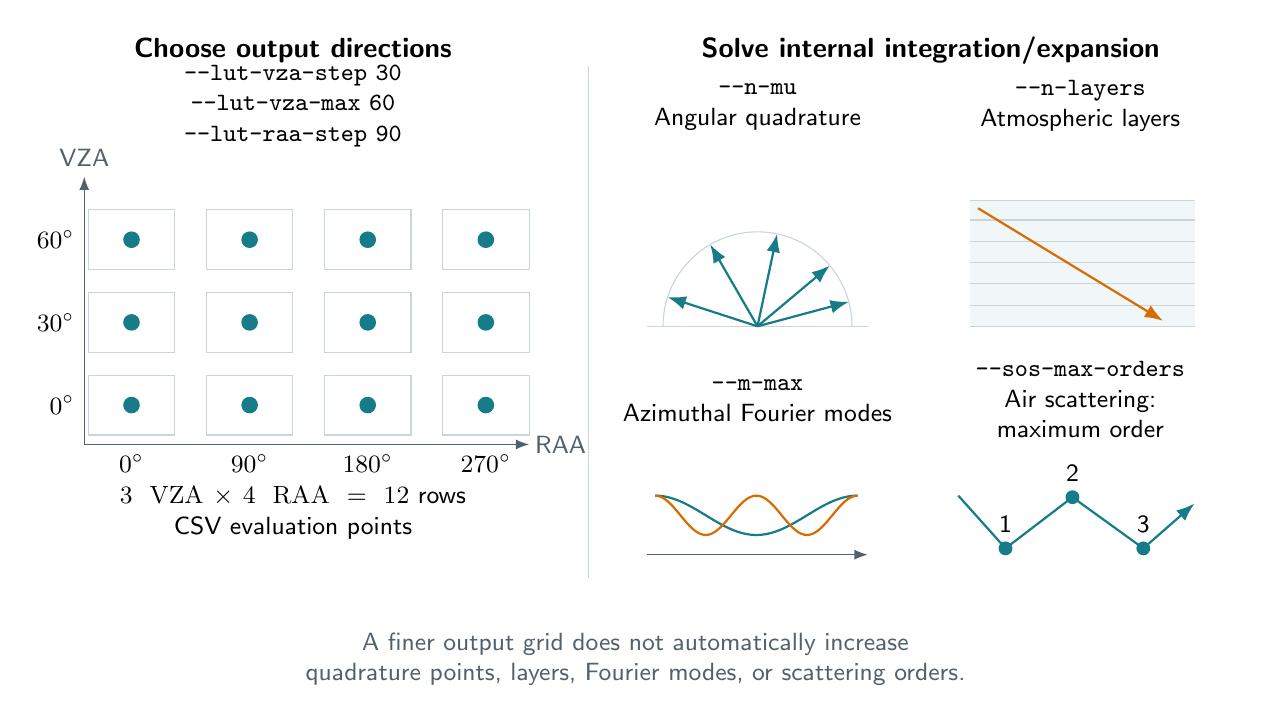
\begin{tikzpicture}[x=1cm,y=1cm,font=\sffamily\fontsize{9}{11}\selectfont,>=Latex]
\node[align=center,font=\sffamily\bfseries\fontsize{10}{12}\selectfont] at (3.35,7.15) {\FigLang{출력할 방향 선택}{Choose output directions}};
\node[align=center,font=\sffamily\bfseries\fontsize{10}{12}\selectfont] at (11.45,7.15) {\FigLang{내부 적분과 전개 계산}{Solve internal integration/expansion}};
\node[align=center,text width=6.4cm] at (3.35,6.45) {\texttt{--lut-vza-step 30}\\\texttt{--lut-vza-max 60}\\\texttt{--lut-raa-step 90}};
\draw[->,ocrtGray] (0.7,2.15)--(6.35,2.15) node[right,inner xsep=2pt] {RAA};
\draw[->,ocrtGray] (0.7,2.15)--(0.7,5.55) node[above] {VZA};
\foreach \x/\labelx in {1.3/0,2.8/90,4.3/180,5.8/270}{\node[below] at (\x,2.15) {$\labelx^\circ$};}
\foreach \y/\labely in {2.65/0,3.7/30,4.75/60}{\node[left] at (0.7,\y) {$\labely^\circ$};}
\foreach \x in {1.3,2.8,4.3,5.8}{\foreach \y in {2.65,3.7,4.75}{\draw[ocrtLine] (\x-0.55,\y-0.38) rectangle +(1.1,0.76);\fill[ocrtTeal] (\x,\y) circle (3pt);}}
\node[align=center,text width=6.2cm] at (3.35,1.28) {$3\;\mathrm{VZA}\times4\;\mathrm{RAA}=12$\FigLang{행}{ rows}\\\FigLang{CSV 평가점}{CSV evaluation points}};
\draw[ocrtLine] (7.1,0.45)--(7.1,6.95);
% Internal quadrature nodes: illustrative positions, not actual Gauss nodes.
\node[align=center] at (9.25,6.45) {\texttt{--n-mu}\\\FigLang{각도 적분점}{Angular quadrature}};
\draw[ocrtLine] (7.85,3.65)--(10.65,3.65);
\draw[ocrtLine] (10.45,3.65) arc[start angle=0,end angle=180,radius=1.2];
\foreach \ang in {15,40,78,120,162}{\draw[->,ocrtTeal,thick] (9.25,3.65)--+(\ang:1.2);}
\node[align=center] at (13.35,6.45) {\texttt{--n-layers}\\\FigLang{대기 수직층}{Atmospheric layers}};
\fill[ocrtTeal!6] (11.95,3.65) rectangle (14.8,5.25);
\foreach \yy in {3.65,3.92,4.19,4.46,4.73,5.0,5.25}{\draw[ocrtLine] (11.95,\yy)--(14.8,\yy);}
\draw[->,orange!85!black,thick] (12.05,5.15)--(14.4,3.72);
\node[align=center,text width=3.9cm] at (9.25,2.72) {\texttt{--m-max}\\\FigLang{방위각 Fourier 모드}{Azimuthal Fourier modes}};
\draw[->,ocrtGray] (7.85,0.75)--(10.65,0.75);
\draw[ocrtTeal,thick,domain=0:360,samples=50] plot ({7.95+\x/140},{1.25+0.25*cos(\x)});
\draw[orange!85!black,thick,domain=0:360,samples=65] plot ({7.95+\x/140},{1.25+0.25*cos(2*\x)});
\node[align=center,text width=4.1cm] at (13.35,2.72) {\texttt{--sos-max-orders}\\\FigLang{최대 대기 산란 차수}{Air scattering:\\maximum order}};
\draw[->,ocrtTeal,thick] (11.8,1.5)--(12.4,0.83)--(13.25,1.48)--(14.15,0.83)--(14.8,1.4);
\foreach \x/\y/\num in {12.4/0.83/1,13.25/1.48/2,14.15/0.83/3}{\fill[ocrtTeal] (\x,\y) circle (2.5pt);\node[above] at (\x,\y+0.08) {\num};}
\node[anchor=north,align=center,text width=15.2cm,text=ocrtGray] at (7.7,-0.12) {\FigLang{출력 격자를 촘촘하게 해도 적분점·층수·Fourier 차수·산란 차수가 자동으로 늘어나지는 않는다.}{A finer output grid does not automatically increase\\quadrature points, layers, Fourier modes, or scattering orders.}};
\end{tikzpicture}
\caption{\FigLang{\texttt{--lut-*}는 CSV에서 평가할 기하를, 수치 옵션은 내부 계산의 해상도와 반복 한계를 정한다. 왼쪽은 12행의 예이며 VZA=0의 네 RAA는 같은 천정 관측을 다른 방위 라벨로 나타낸다. 오른쪽 적분점·층·곡선은 개념도다. \texttt{--n-mu-water}와 \texttt{--water-m-max}는 별도 수중 제어이며 \texttt{--sos-max-orders}가 수중 차수 한계를 바꾸지는 않는다. 명시적인 해양 격자 파일 지정 시 수중 기본 적분점이 96으로 승격되는 현재 구현의 예외는 본문의 설명을 함께 따른다.}{\texttt{--lut-*} chooses geometries evaluated in the CSV; numerical options control internal resolution and iteration limits. The left panel has 12 rows; its four RAA labels at VZA=0 share the zenith viewing direction. Internal nodes, layers, and curves are schematic. \texttt{--n-mu-water} and \texttt{--water-m-max} control underwater calculations separately; \texttt{--sos-max-orders} does not set the underwater order limit. See the text for the current implementation's promotion to 96 underwater nodes when an explicit ocean-grid filename is parsed.}}
\label{fig:options-grids}
\end{figure}


Start ordinary work with the defaults. \texttt{OCRT\_\allowbreak{}ADVANCED=\allowbreak{}1} permits numerical experiments beyond the validated default configuration; it does not automatically guarantee the accuracy of altered settings. Enabling the flag does not automatically change other option values.


\begin{ManualCode}
$env:OCRT_ADVANCED = "1"
\end{ManualCode}


\begin{ManualCode}
export OCRT_ADVANCED=1
\end{ManualCode}


{\TableFont
\begin{longtable}{@{}>{\raggedright\arraybackslash}p{\dimexpr 0.3000\linewidth-5.33pt\relax}>{\raggedright\arraybackslash}p{\dimexpr 0.2300\linewidth-5.33pt\relax}>{\raggedright\arraybackslash}p{\dimexpr 0.4700\linewidth-5.33pt\relax}@{}}
\toprule
\textbf{Option} & \textbf{Default} & \textbf{Actual application / gate} \\
\midrule
\endfirsthead
\toprule
\textbf{Option} & \textbf{Default} & \textbf{Actual application / gate} \\
\midrule
\endhead
\bottomrule
\endfoot
\texttt{-\allowbreak{}-\allowbreak{}n-\allowbreak{}mu N} & \texttt{24} & Atmospheric Gauss--Legendre quadrature count per hemisphere. Integer \texttt{N\ensuremath{\geq}2}. Values other than 24 require ADVANCED. Different from the number of output VZA points. \\
\texttt{-\allowbreak{}-\allowbreak{}n-\allowbreak{}layers N} & \texttt{40} for AOD 0; \texttt{400} for AOD>0 & Atmospheric layer count. Integer \texttt{N\ensuremath{\geq}2}. Departures from the applicable default require ADVANCED. Does not change the underwater layer count. \\
\texttt{-\allowbreak{}-\allowbreak{}m-\allowbreak{}max M} & \texttt{2} for AOD 0; \texttt{16} for AOD>0 & Maximum atmospheric azimuthal Fourier mode. Integer \texttt{0\ensuremath{\leq}M\ensuremath{\leq}32}. Departures from the applicable default require ADVANCED. \\
\texttt{-\allowbreak{}-\allowbreak{}sos-\allowbreak{}max-\allowbreak{}orders N} & \texttt{20} & \textbf{Actual maximum atmospheric SOS scattering order}. \texttt{N\ensuremath{\geq}1}. Values other than 20 require ADVANCED. Separate from automatic underwater order limits. \\
\texttt{-\allowbreak{}-\allowbreak{}sos-\allowbreak{}tolerance X} & \texttt{1e-\allowbreak{}7} & \textbf{Actual atmospheric SOS convergence tolerance}, positive. Departures from the default require ADVANCED. \\
\texttt{-\allowbreak{}-\allowbreak{}sos-\allowbreak{}acceleration STR\allowbreak{}} & \texttt{plain} & Only \texttt{plain} is implemented. \texttt{geometric} produces an explicit not-implemented error. \\
\texttt{-\allowbreak{}-\allowbreak{}integration-\allowbreak{}method STR} & \texttt{linear} & Linear integration of the source within a layer. \texttt{constant} is diagnostic and requires DEBUG. \\
\texttt{-\allowbreak{}-\allowbreak{}n-\allowbreak{}mu-\allowbreak{}water N} & \texttt{48} for ordinary underwater runs; \texttt{96} for explicit ocean grids & Underwater \ensuremath{\mu} quadrature count per hemisphere. Positive integer. \textbf{Explicit use always requires ADVANCED}. Do not reduce the count for large-scale calculations without checking convergence. \\
\texttt{-\allowbreak{}-\allowbreak{}n-\allowbreak{}mu-\allowbreak{}water-\allowbreak{}sky N} & \texttt{0} = default underwater grid & Diagnostic numerical option selecting a smaller underwater quadrature count only for the coupling path of incoming atmospheric sky beams. Separate from the direct solar-beam grid, and consumed only by some coupled paths. No current CLI gate. \\
\texttt{-\allowbreak{}-\allowbreak{}water-\allowbreak{}m-\allowbreak{}max M} & Automatic & Overrides the underwater Fourier-mode upper limit with a positive value. Explicit use always requires ADVANCED. 0 does not override the actual solver. \\
\texttt{-\allowbreak{}-\allowbreak{}water-\allowbreak{}shared-\allowbreak{}grid} & OFF & Matches the underwater quadrature count to atmospheric \texttt{-\allowbreak{}-\allowbreak{}n-\allowbreak{}mu}. Sharing the default atmospheric value 24 reduces it below the independent underwater defaults 48/96, so convergence must be checked for comparisons. Do not combine with \texttt{-\allowbreak{}-\allowbreak{}n-\allowbreak{}mu-\allowbreak{}water}. \\
\texttt{-\allowbreak{}-\allowbreak{}water-\allowbreak{}view-\allowbreak{}as-\allowbreak{}node} & Currently ON in the CLI & Enables node extraction for the requested underwater viewing direction. The help's “default OFF” differs from the current initial value. \\
\texttt{-\allowbreak{}-\allowbreak{}water-\allowbreak{}view-\allowbreak{}as-\allowbreak{}node-\allowbreak{}off} & Default OFF & Diagnostic option disabling node extraction in a single case to compare the continuous reconstruction/interpolation path. Distinguish this from the grid's own multiple-viewing-node processing. \\
\texttt{-\allowbreak{}-\allowbreak{}sigma-\allowbreak{}model STR} & \texttt{ocrt-\allowbreak{}floor} & Sea-surface slope-variance formula. \texttt{ocrt\_\allowbreak{}floor} is also recognized. \texttt{nakajima-\allowbreak{}tanaka}/\texttt{nakajima\_\allowbreak{}tanaka} requires ADVANCED. \\
\texttt{-\allowbreak{}-\allowbreak{}sigma-\allowbreak{}type N} & \texttt{1} & Compatible numeric selection of the model above. \texttt{1}: OCRT floor; \texttt{0}: Nakajima--Tanaka. Values other than 1 require ADVANCED. Use the string option in new commands. \\
\texttt{-\allowbreak{}-\allowbreak{}q-\allowbreak{}convention N} & \texttt{1} & Fresnel-boundary Q convention. \texttt{1}: \texttt{(Rp-Rs)/\allowbreak{}2}; \texttt{0}: the older \texttt{(Rs-Rp)/\allowbreak{}2}. Values other than 1 require ADVANCED. Do not treat this as a post-processing option that simply reverses every output Q. \\
\end{longtable}
}

The implemented slope variance is \texttt{0.\allowbreak{}003+0.\allowbreak{}00512\ensuremath{\times}max(0.\allowbreak{}01,\allowbreak{}U)} for OCRT floor and \texttt{(0.\allowbreak{}0731\ensuremath{\sqrt{}}max(0,\allowbreak{}U))\textsuperscript{2}} for Nakajima--Tanaka. The upper-level path selects the flat Fresnel branch at wind speed 0, so do not interpret results at wind speed 0 solely through the rough-surface slope-variance formula.

The following three options remain in the parser, but \textbf{their effect in current runs is not equivalent to that of other numerical options}.


{\TableFont
\begin{longtable}{@{}>{\raggedright\arraybackslash}p{\dimexpr 0.3000\linewidth-5.33pt\relax}>{\raggedright\arraybackslash}p{\dimexpr 0.2300\linewidth-5.33pt\relax}>{\raggedright\arraybackslash}p{\dimexpr 0.4700\linewidth-5.33pt\relax}@{}}
\toprule
\textbf{Option} & \textbf{Default / gate} & \textbf{Current status} \\
\midrule
\endfirsthead
\toprule
\textbf{Option} & \textbf{Default / gate} & \textbf{Current status} \\
\midrule
\endhead
\bottomrule
\endfoot
\texttt{-\allowbreak{}-\allowbreak{}max-\allowbreak{}orders N} & Default \texttt{20}; changes require ADVANCED & Stored in the legacy \texttt{opts.\allowbreak{}max\_\allowbreak{}orders} field. The current atmospheric solver limits orders with \texttt{opts.\allowbreak{}sos.\allowbreak{}max\_\allowbreak{}iterations}. Use \texttt{-\allowbreak{}-\allowbreak{}sos-\allowbreak{}max-\allowbreak{}orders} for actual control. \\
\texttt{-\allowbreak{}-\allowbreak{}conv-\allowbreak{}tol X} & Default \texttt{1e-\allowbreak{}6}; changes require ADVANCED & Stored in legacy \texttt{opts.\allowbreak{}conv\_\allowbreak{}tol}. Current atmospheric SOS uses \texttt{-\allowbreak{}-\allowbreak{}sos-\allowbreak{}tolerance}. \\
\texttt{-\allowbreak{}-\allowbreak{}l-\allowbreak{}max auto\textbackslash{}|N} & Default \texttt{auto}; numeric specification requires ADVANCED & The current atmospheric solver determines its working order from the Fourier upper limit, Rayleigh order, and aerosol L rather than \texttt{opts.\allowbreak{}l\_\allowbreak{}max}. Do not confuse this with \texttt{-\allowbreak{}-\allowbreak{}aer-\allowbreak{}l-\allowbreak{}max}. \\
\end{longtable}
}

The default maximum underwater order depends on the medium. The ordinary pure-water path starts at 20, the constituent path at a minimum of 140, and the direct IOP path at a minimum of 160. Positive particulate constituents, direct IOP \texttt{b>0.\allowbreak{}02 m\textsuperscript{-}\textsuperscript{1}}, or \texttt{bb>0.\allowbreak{}0005 m\textsuperscript{-}\textsuperscript{1}} raise it again to the current code's high-particle safety floor of \textbf{10000}. The older comment's 100 differs from the actual constant. The solver need not iterate to the limit: it exits early upon convergence. Additional automatic policies apply to depth and phase processing. Check the actual \texttt{water\_\allowbreak{}orders} and \texttt{water\_\allowbreak{}converged} in logs/output. Do not expect increasing only \texttt{-\allowbreak{}-\allowbreak{}sos-\allowbreak{}max-\allowbreak{}orders} to resolve underwater nonconvergence.

\section{Complete Diagnostic Option List}
\label{sec:auto:03_options:9}
DEBUG options are allowed by the \texttt{OCRT\_\allowbreak{}DEBUG=\allowbreak{}1} environment variable or \texttt{-\allowbreak{}-\allowbreak{}debug} at the beginning of the command. \texttt{-\allowbreak{}-\allowbreak{}debug} takes effect when encountered, so put it before related options. DEBUG and ADVANCED are separate; set both when both gates are required.


{\TableFont
\begin{longtable}{@{}>{\raggedright\arraybackslash}p{\dimexpr 0.3000\linewidth-5.33pt\relax}>{\raggedright\arraybackslash}p{\dimexpr 0.2300\linewidth-5.33pt\relax}>{\raggedright\arraybackslash}p{\dimexpr 0.4700\linewidth-5.33pt\relax}@{}}
\toprule
\textbf{Option} & \textbf{Value / default} & \textbf{Purpose / conditions} \\
\midrule
\endfirsthead
\toprule
\textbf{Option} & \textbf{Value / default} & \textbf{Purpose / conditions} \\
\midrule
\endhead
\bottomrule
\endfoot
\texttt{-\allowbreak{}-\allowbreak{}debug} & Flag & Sets \texttt{OCRT\_\allowbreak{}DEBUG=\allowbreak{}1} for the process. Omit from ordinary production data-generation commands. \\
\texttt{-\allowbreak{}-\allowbreak{}debug-\allowbreak{}fixed-\allowbreak{}bulk-\allowbreak{}lmax N} & 0 = automatic for each path & Maximum moment order of the IOP fixed bulk phase function. DEBUG; IOP model. Automatic values include 200 for Mie paths and 30 for LUT paths, so do not assume equal orders. \\
\texttt{-\allowbreak{}-\allowbreak{}debug-\allowbreak{}fixed-\allowbreak{}bulk-\allowbreak{}phase-\allowbreak{}model M} & Internal \texttt{delta2bb} & IOP diagnostic phase selection. Aliases of \texttt{delta2bb}: \texttt{delta}, \texttt{bb2}; of \texttt{hg-\allowbreak{}lut}: \texttt{hg\_\allowbreak{}direct}, \texttt{hg}; of \texttt{lut}: \texttt{table}, \texttt{p11-\allowbreak{}lut}; of \texttt{lut-\allowbreak{}deltam}: \texttt{deltam}, \texttt{delta-\allowbreak{}m}. DEBUG. LUT selections require a phase file. \\
\texttt{-\allowbreak{}-\allowbreak{}debug-\allowbreak{}high-\allowbreak{}particle-\allowbreak{}water-\allowbreak{}max-\allowbreak{}orders N} & Current safety floor \texttt{10000} when unspecified & Minimum SOS order limit for a particulate medium. Positive integer; DEBUG. Does not lower a model already requiring 140/160 below that requirement. \\
\texttt{-\allowbreak{}-\allowbreak{}debug-\allowbreak{}water-\allowbreak{}max-\allowbreak{}orders N} & Automatic & Directly changes the underwater SOS upper order limit. Positive integer; DEBUG. If reduced, check actual results for nonconvergence. \\
\texttt{-\allowbreak{}-\allowbreak{}debug-\allowbreak{}water-\allowbreak{}tau-\allowbreak{}max-\allowbreak{}target X} & Automatic by medium & Baseline target total underwater optical thickness. Positive, dimensionless; DEBUG. Deep-water policy may adjust final depth further. \\
\texttt{-\allowbreak{}-\allowbreak{}debug-\allowbreak{}water-\allowbreak{}max-\allowbreak{}tau X} & Automatic by medium & Final upper limit on underwater optical thickness. Positive, dimensionless; DEBUG. \\
\texttt{-\allowbreak{}-\allowbreak{}debug-\allowbreak{}water-\allowbreak{}max-\allowbreak{}depth X} & Automatic by medium & Upper limit on physical underwater depth, m, positive; DEBUG. Not a general water-depth/seabed-reflection model input. \\
\texttt{-\allowbreak{}-\allowbreak{}debug-\allowbreak{}water-\allowbreak{}min-\allowbreak{}depth X} & Same as above & Legacy alias stored in exactly the same field as \texttt{-\allowbreak{}-\allowbreak{}debug-\allowbreak{}water-\allowbreak{}max-\allowbreak{}depth} in the current code. Despite its name, it does not specify a minimum depth. \\
\texttt{-\allowbreak{}-\allowbreak{}debug-\allowbreak{}water-\allowbreak{}bottom-\allowbreak{}tol X} & \texttt{1e-\allowbreak{}8} & Target transport attenuation to the bottom. \texttt{0<X<1}; DEBUG. \\
\texttt{-\allowbreak{}-\allowbreak{}debug-\allowbreak{}water-\allowbreak{}layer-\allowbreak{}dtau X} & \texttt{0.\allowbreak{}05} & Target optical thickness per layer, positive; DEBUG. \\
\texttt{-\allowbreak{}-\allowbreak{}debug-\allowbreak{}water-\allowbreak{}n-\allowbreak{}layers N} & Automatic & Fixes the underwater layer count, positive integer; DEBUG. Disables automatic \ensuremath{\Delta}\ensuremath{\tau}-based layer-count increases when specified. \\
\texttt{-\allowbreak{}-\allowbreak{}ccrr-\allowbreak{}particle-\allowbreak{}phase-\allowbreak{}lut FILE} & None & Replacement scalar LUT for the CCRR particle phase. DEBUG. Chl or TSM>0; mutually exclusive with \texttt{-\allowbreak{}-\allowbreak{}ccrr-\allowbreak{}phase-\allowbreak{}moments}. \\
\texttt{-\allowbreak{}-\allowbreak{}ccrr-\allowbreak{}particle-\allowbreak{}phase-\allowbreak{}case-\allowbreak{}id ID} & None & Case ID to select in the LUT above. DEBUG; requires the LUT option. \\
\texttt{-\allowbreak{}-\allowbreak{}ccrr-\allowbreak{}particle-\allowbreak{}phase-\allowbreak{}lmax N} & \texttt{10} & Moment order for the LUT above, positive; DEBUG; requires the LUT option. \\
\texttt{-\allowbreak{}-\allowbreak{}ccrr-\allowbreak{}particle-\allowbreak{}phase-\allowbreak{}nphi N} & \texttt{720} & Azimuthal integration count for the LUT above, positive; DEBUG; requires the LUT option. \\
\texttt{-\allowbreak{}-\allowbreak{}trunc-\allowbreak{}aer-\allowbreak{}fit DEG} & OFF & Boundary angle in degrees for research aerosol delta-fit truncation. DEBUG; AOD>0. \\
\texttt{-\allowbreak{}-\allowbreak{}trunc-\allowbreak{}aer-\allowbreak{}m N} & OFF & Research aerosol delta-M truncation order. DEBUG; AOD>0. Use as an experiment distinct from the option above. \\
\texttt{-\allowbreak{}-\allowbreak{}nt-\allowbreak{}tau} & OFF & NT optical-thickness/albedo transformation for research truncation. DEBUG; AOD>0. Do not assume the same physics as the normal automatic loglin path. \\
\texttt{-\allowbreak{}-\allowbreak{}sos-\allowbreak{}save-\allowbreak{}orders} & OFF & DEBUG. The current parser sets the \texttt{save\_\allowbreak{}orders} field, but production SOS does not read it to write separate files by order. Do not expect this option alone to create order-resolved output files. \\
\texttt{-\allowbreak{}-\allowbreak{}ccrr-\allowbreak{}compare FILE}, \texttt{-\allowbreak{}-\allowbreak{}simple-\allowbreak{}compare FILE} & None & Diagnostic comparison against CCRR reference CSV. DEBUG. Cannot be mixed with a single \texttt{-\allowbreak{}-\allowbreak{}water-\allowbreak{}model} branch. \\
\texttt{-\allowbreak{}-\allowbreak{}ccrr-\allowbreak{}output FILE}, \texttt{-\allowbreak{}-\allowbreak{}simple-\allowbreak{}output FILE} & None & Output file for the comparison above. Uses \texttt{-\allowbreak{}-\allowbreak{}output} if unspecified. Errors if neither path is provided. \\
\end{longtable}
}

\subsection{Fournier--Forand Scalar Phase Research Path}
\label{sec:auto:03_options:9.1}
The following is a research path within \texttt{-\allowbreak{}-\allowbreak{}water-\allowbreak{}model iop}, not an independent model added to the ordinary water-model choices. It can read a,b from a table and calculate bb from a user-specified backscattering ratio.


{\TableFont
\begin{longtable}{@{}>{\raggedright\arraybackslash}p{\dimexpr 0.3000\linewidth-5.33pt\relax}>{\raggedright\arraybackslash}p{\dimexpr 0.2300\linewidth-5.33pt\relax}>{\raggedright\arraybackslash}p{\dimexpr 0.4700\linewidth-5.33pt\relax}@{}}
\toprule
\textbf{Option and all aliases} & \textbf{Value / default} & \textbf{Description} \\
\midrule
\endfirsthead
\toprule
\textbf{Option and all aliases} & \textbf{Value / default} & \textbf{Description} \\
\midrule
\endhead
\bottomrule
\endfoot
\texttt{-\allowbreak{}-\allowbreak{}scalar-\allowbreak{}ff-\allowbreak{}iop FILE}, \texttt{-\allowbreak{}-\allowbreak{}ff-\allowbreak{}iop FILE}, \texttt{-\allowbreak{}-\allowbreak{}ff-\allowbreak{}scalar-\allowbreak{}iop FILE} & None & \texttt{wavelength\_\allowbreak{}nm,\allowbreak{}a,\allowbreak{}b} table. DEBUG. The run wavelength must lie within the table range; interpolation is linear, without extrapolation. This file replaces the requirement for \texttt{-\allowbreak{}-\allowbreak{}iop-\allowbreak{}a/\allowbreak{}b/\allowbreak{}bb}. \\
\texttt{-\allowbreak{}-\allowbreak{}scalar-\allowbreak{}ff-\allowbreak{}bbfrac X}, \texttt{-\allowbreak{}-\allowbreak{}scalar-\allowbreak{}ff-\allowbreak{}bb-\allowbreak{}over-\allowbreak{}b X}, \texttt{-\allowbreak{}-\allowbreak{}ff-\allowbreak{}bbfrac X} & Unspecified \texttt{0} & bb/b with \texttt{0<X<0.\allowbreak{}5}. Required for the file path. \\
\texttt{-\allowbreak{}-\allowbreak{}scalar-\allowbreak{}ff-\allowbreak{}n X}, \texttt{-\allowbreak{}-\allowbreak{}ff-\allowbreak{}n X} & \texttt{1.\allowbreak{}18} & FF particle relative refractive index \texttt{>1}. \\
\texttt{-\allowbreak{}-\allowbreak{}scalar-\allowbreak{}ff-\allowbreak{}mu X}, \texttt{-\allowbreak{}-\allowbreak{}ff-\allowbreak{}mu X} & Automatic & Junge exponent. Estimated from bb/b if unspecified; when supplied directly, use a valid FF exponent (\texttt{>3}). \\
\texttt{-\allowbreak{}-\allowbreak{}scalar-\allowbreak{}ff-\allowbreak{}lmax N}, \texttt{-\allowbreak{}-\allowbreak{}ff-\allowbreak{}lmax N} & \texttt{10} in the file path & Retained FF moment order. Positive integer. \\
\texttt{-\allowbreak{}-\allowbreak{}scalar-\allowbreak{}ff-\allowbreak{}phase-\allowbreak{}nphi N}, \texttt{-\allowbreak{}-\allowbreak{}scalar-\allowbreak{}ff-\allowbreak{}nphi N}, \texttt{-\allowbreak{}-\allowbreak{}ff-\allowbreak{}phase-\allowbreak{}nphi N}, \texttt{-\allowbreak{}-\allowbreak{}ff-\allowbreak{}nphi N} & \texttt{720} & FF azimuthal integration count. Explicit use always requires ADVANCED. \\
\end{longtable}
}

The current implementation requires DEBUG for the FF file option and ADVANCED for nphi, but has no individual DEBUG gates for the other FF parameters. Nevertheless, this group is a diagnostic path: do not mix only some of its flags into ordinary IOP calculations and expect them to apply.

\section{Run Information and Environment Variables}
\label{sec:auto:03_options:10}

{\TableFont
\begin{longtable}{@{}>{\raggedright\arraybackslash}p{\dimexpr 0.3400\linewidth-4.00pt\relax}>{\raggedright\arraybackslash}p{\dimexpr 0.6600\linewidth-4.00pt\relax}@{}}
\toprule
\textbf{Option} & \textbf{Behavior} \\
\midrule
\endfirsthead
\toprule
\textbf{Option} & \textbf{Behavior} \\
\midrule
\endhead
\bottomrule
\endfoot
\texttt{-\allowbreak{}-\allowbreak{}help}, \texttt{-\allowbreak{}h} & Prints general help and exits. Does not enumerate every hidden numerical/diagnostic option. \\
\texttt{-\allowbreak{}-\allowbreak{}examples} & Prints older validation run examples embedded in the program and exits. Prefer Appendix~\ref{chap:04_examples} for current reproducible examples. \\
\texttt{-\allowbreak{}-\allowbreak{}version} & Prints the build string and exits. The repository release number may differ from the string's old \texttt{v1.\allowbreak{}2} label, so also record the source revision. \\
\texttt{-\allowbreak{}-\allowbreak{}verbose} & Prints additional run information, default-selection details, and aerosol diagnostics to standard error. Store file data separately from logs. \\
\end{longtable}
}

The following environment variables are used in actual operation. Unless stated otherwise, set them before starting the program. Variables left in the same shell can affect later runs. Some internal diagnostic variables treat even the string \texttt{0} as “present,” so remove the variable to turn them off.


{\TableFont
\begin{longtable}{@{}>{\raggedright\arraybackslash}p{\dimexpr 0.3000\linewidth-5.33pt\relax}>{\raggedright\arraybackslash}p{\dimexpr 0.2300\linewidth-5.33pt\relax}>{\raggedright\arraybackslash}p{\dimexpr 0.4700\linewidth-5.33pt\relax}@{}}
\toprule
\textbf{Environment variable} & \textbf{Value / default} & \textbf{Purpose} \\
\midrule
\endfirsthead
\toprule
\textbf{Environment variable} & \textbf{Value / default} & \textbf{Purpose} \\
\midrule
\endhead
\bottomrule
\endfoot
\texttt{OMP\_\allowbreak{}NUM\_\allowbreak{}THREADS} & Positive integer; OpenMP runtime default & Number of OpenMP workers. Start reproducibility comparisons at \texttt{1}. The build must support OpenMP. \\
\texttt{OCRT\_\allowbreak{}ADVANCED} & OFF when unset; usually \texttt{1} & ADVANCED gate in the tables above. \\
\texttt{OCRT\_\allowbreak{}DEBUG} & OFF when unset; usually \texttt{1} & DEBUG gate in the tables above. Can also be set with \texttt{-\allowbreak{}-\allowbreak{}debug}. \\
\texttt{OCRT\_\allowbreak{}TSM\_\allowbreak{}DIR} & Searches distributed TSM locations when unset & Overrides the Ahn inorganic-particle data directory. All required coefficients and phase files for the four species must be present. \\
\texttt{OCRT\_\allowbreak{}ORGANIC\_\allowbreak{}DIR} & Searches distributed organic-particle locations when unset & Overrides the organic-particle data directory. Requires common phytoplankton absorption and detritus data. \\
\texttt{OCRT\_\allowbreak{}SURFACE\_\allowbreak{}PERSIST\_\allowbreak{}CACHE\_\allowbreak{}MODE} & Default \texttt{off} & Sea-surface kernel disk cache. \texttt{readonly}: reads, calculates on a miss; \texttt{required}: errors if a required cache is absent; \texttt{build}: calculates and saves. Aliases: \texttt{0}; \texttt{read-\allowbreak{}only/\allowbreak{}ro/\allowbreak{}optional}; \texttt{require/\allowbreak{}strict}; \texttt{prime/\allowbreak{}prebuild}. \\
\texttt{OCRT\_\allowbreak{}SURFACE\_\allowbreak{}PERSIST\_\allowbreak{}CACHE\_\allowbreak{}DIR} & Required when cache is ON & Cache directory. Create it and check write permission before use. \\
\texttt{OCRT\_\allowbreak{}SURFACE\_\allowbreak{}PERSIST\_\allowbreak{}CACHE\_\allowbreak{}TRACE} & Default OFF; \texttt{1} & Cache hit/miss and configuration diagnostics. \\
\texttt{OCRT\_\allowbreak{}WATER\_\allowbreak{}VALUE\_\allowbreak{}GEOM\_\allowbreak{}CACHE\_\allowbreak{}MAX\_\allowbreak{}MB} & Default \texttt{64} MiB; maximum \texttt{4096} & Value-kernel geometry cache size. \texttt{0} suppresses allocation. \\
\texttt{OCRT\_\allowbreak{}COXMUNK\_\allowbreak{}FOURIER\_\allowbreak{}NPHI} & Default \texttt{1024} & Azimuthal quadrature count for rough-surface Fourier integration. Integer override \texttt{64.\allowbreak{}.\allowbreak{}4096}. For convergence comparisons. \\
\texttt{OCRT\_\allowbreak{}IPSS\_\allowbreak{}NQUAD} & Current default \texttt{2} per layer panel & IPSS path-integration convergence comparisons. Does not mean only 2 points along the entire line of sight. Overrides accept integers \texttt{8.\allowbreak{}.\allowbreak{}4096} only; out-of-range values retain the default. \\
\texttt{OCRT\_\allowbreak{}IPSS\_\allowbreak{}TRACE} & OFF when unset & IPSS correction diagnostics. \\
\texttt{OCRT\_\allowbreak{}IPSS\_\allowbreak{}DUMP} & None when unset; output file path & Appends IPSS grid diagnostics to a file. 6 columns without a header: \texttt{vza,\allowbreak{}raa,\allowbreak{}kappa,\allowbreak{}i\_\allowbreak{}nadir/\allowbreak{}i\_\allowbreak{}pp,\allowbreak{}i\_\allowbreak{}spherical,\allowbreak{}i\_\allowbreak{}pp}. Use a new filename for each run to avoid mixing with previous results. \\
\texttt{OCRT\_\allowbreak{}IPSS\_\allowbreak{}PROFILE\_\allowbreak{}DUMP} & None when unset; output file path & Writes IPSS atmospheric-profile and phase-function diagnostics to the specified file. \\
\end{longtable}
}

Performance/regression diagnostic variables include \texttt{OCRT\_\allowbreak{}TRANSPORT\_\allowbreak{}CACHE\_\allowbreak{}OFF}, \texttt{OCRT\_\allowbreak{}SOS\_\allowbreak{}ZERO\_\allowbreak{}COL\_\allowbreak{}SKIP\_\allowbreak{}OFF}, \texttt{OCRT\_\allowbreak{}DISABLE\_\allowbreak{}MIE\_\allowbreak{}MODEL\_\allowbreak{}CACHE}, \texttt{OCRT\_\allowbreak{}DISABLE\_\allowbreak{}WATER\_\allowbreak{}COMPONENT\_\allowbreak{}PHASE\_\allowbreak{}CACHE}, \texttt{OCRT\_\allowbreak{}AIR\_\allowbreak{}SURFACE\_\allowbreak{}CACHE\_\allowbreak{}OFF}, \texttt{OCRT\_\allowbreak{}AIR\_\allowbreak{}FKC\_\allowbreak{}OFF}, \texttt{OCRT\_\allowbreak{}TWA\_\allowbreak{}FKC\_\allowbreak{}OFF}, and \texttt{OCRT\_\allowbreak{}NO\_\allowbreak{}PHASE\_\allowbreak{}CACHE}. They disable specific caches or skip optimizations to compare result equivalence and timing. \texttt{OCRT\_\allowbreak{}MIE\_\allowbreak{}MODEL\_\allowbreak{}CACHE\_\allowbreak{}TRACE}, \texttt{OCRT\_\allowbreak{}DUMP\_\allowbreak{}WATER\_\allowbreak{}COMPONENT\_\allowbreak{}PHASE\_\allowbreak{}CACHE}, \texttt{OCRT\_\allowbreak{}DUMP\_\allowbreak{}SOS\_\allowbreak{}PHASE\_\allowbreak{}CACHE}, \texttt{OCRT\_\allowbreak{}AIR\_\allowbreak{}SURFACE\_\allowbreak{}CACHE\_\allowbreak{}DIAG}, \texttt{OCRT\_\allowbreak{}VALUE\_\allowbreak{}GEOM\_\allowbreak{}CACHE\_\allowbreak{}TRACE}, \texttt{OCRT\_\allowbreak{}VALUE\_\allowbreak{}KERNEL\_\allowbreak{}CACHE\_\allowbreak{}TRACE}, and \texttt{OCRT\_\allowbreak{}BATCH\_\allowbreak{}DIAG} produce the corresponding diagnostics.

Other source variables such as \texttt{OCRT\_\allowbreak{}DUMP\_\allowbreak{}*}, \texttt{OCRT\_\allowbreak{}D3\_\allowbreak{}*}, \texttt{OCRT\_\allowbreak{}TWA\_\allowbreak{}*}, \texttt{OCRT\_\allowbreak{}DTP\_\allowbreak{}*}, and \texttt{OCRT\_\allowbreak{}FINAL\_\allowbreak{}MODE\_\allowbreak{}QUEUE\_\allowbreak{}*} serve internal cause-isolation and modification experiments; they are not stable user options. Some change solver paths or physical terms rather than merely adding output. Do not copy all environment variables from an old validation script into a new production command. The \hyperref[chap:03_environment_index]{environment-variable source index} lists the read locations of all internal variables.

\section{Removed Options and Replacements}
\label{sec:auto:03_options:11}
The current parser explicitly rejects the names below. Reproducing commands from older documents requires checking surface and physical defaults as well as substituting names.


{\TableFont
\begin{longtable}{@{}>{\raggedright\arraybackslash}p{\dimexpr 0.3400\linewidth-4.00pt\relax}>{\raggedright\arraybackslash}p{\dimexpr 0.6600\linewidth-4.00pt\relax}@{}}
\toprule
\textbf{Rejected name} & \textbf{Replacement or current meaning} \\
\midrule
\endfirsthead
\toprule
\textbf{Rejected name} & \textbf{Replacement or current meaning} \\
\midrule
\endhead
\bottomrule
\endfoot
\texttt{-\allowbreak{}-\allowbreak{}cdom-\allowbreak{}a440}, \texttt{-\allowbreak{}-\allowbreak{}cdom-\allowbreak{}slope}, \texttt{-\allowbreak{}-\allowbreak{}cdom-\allowbreak{}ref-\allowbreak{}lambda} & \texttt{-\allowbreak{}-\allowbreak{}water-\allowbreak{}model ocrt}/\texttt{ccrr} with \texttt{-\allowbreak{}-\allowbreak{}ocrt-\allowbreak{}adom440}/\texttt{-\allowbreak{}-\allowbreak{}ccrr-\allowbreak{}adom440} and the corresponding slope. Reference wavelength fixed at 440 nm. \\
\texttt{-\allowbreak{}-\allowbreak{}simple-\allowbreak{}mode}, \texttt{-\allowbreak{}-\allowbreak{}ccrr-\allowbreak{}mode} & \texttt{-\allowbreak{}-\allowbreak{}water-\allowbreak{}model ocrt\textbackslash{}|ccrr\allowbreak{}\textbackslash{}|iop} \\
\texttt{-\allowbreak{}-\allowbreak{}chl}, \texttt{-\allowbreak{}-\allowbreak{}simple-\allowbreak{}chl}, \texttt{-\allowbreak{}-\allowbreak{}ccrr-\allowbreak{}chl-\allowbreak{}mg-\allowbreak{}m3} & Model-appropriate \texttt{-\allowbreak{}-\allowbreak{}ocrt-\allowbreak{}chl} or \texttt{-\allowbreak{}-\allowbreak{}ccrr-\allowbreak{}chl} \\
\texttt{-\allowbreak{}-\allowbreak{}tsm}, \texttt{-\allowbreak{}-\allowbreak{}simple-\allowbreak{}min}, \texttt{-\allowbreak{}-\allowbreak{}ccrr-\allowbreak{}min}, \texttt{-\allowbreak{}-\allowbreak{}ccrr-\allowbreak{}min-\allowbreak{}g-\allowbreak{}m3} & \texttt{-\allowbreak{}-\allowbreak{}ocrt-\allowbreak{}tsm} or \texttt{-\allowbreak{}-\allowbreak{}ccrr-\allowbreak{}tsm} \\
\texttt{-\allowbreak{}-\allowbreak{}adom440}, \texttt{-\allowbreak{}-\allowbreak{}simple-\allowbreak{}adom440}, \texttt{-\allowbreak{}-\allowbreak{}ccrr-\allowbreak{}adom-\allowbreak{}440} & \texttt{-\allowbreak{}-\allowbreak{}ocrt-\allowbreak{}adom440} or \texttt{-\allowbreak{}-\allowbreak{}ccrr-\allowbreak{}adom440} \\
\texttt{-\allowbreak{}-\allowbreak{}adom-\allowbreak{}slope}, \texttt{-\allowbreak{}-\allowbreak{}simple-\allowbreak{}adom-\allowbreak{}s}, \texttt{-\allowbreak{}-\allowbreak{}simple-\allowbreak{}adom-\allowbreak{}slope}, \texttt{-\allowbreak{}-\allowbreak{}ccrr-\allowbreak{}adom-\allowbreak{}s} & \texttt{-\allowbreak{}-\allowbreak{}ocrt-\allowbreak{}adom-\allowbreak{}slope} or \texttt{-\allowbreak{}-\allowbreak{}ccrr-\allowbreak{}adom-\allowbreak{}slope} \\
\texttt{-\allowbreak{}-\allowbreak{}phyto-\allowbreak{}group}, \texttt{-\allowbreak{}-\allowbreak{}chl-\allowbreak{}group} & Older names for species selection. Omit: current \texttt{-\allowbreak{}-\allowbreak{}ocrt-\allowbreak{}phyto-\allowbreak{}group} is also inactive in the production path. \\
\texttt{-\allowbreak{}-\allowbreak{}tsm-\allowbreak{}species} & \texttt{-\allowbreak{}-\allowbreak{}ocrt-\allowbreak{}tsm-\allowbreak{}species} \\
\texttt{-\allowbreak{}-\allowbreak{}detritus-\allowbreak{}a440}, \texttt{-\allowbreak{}-\allowbreak{}detritus-\allowbreak{}slope} & \texttt{-\allowbreak{}-\allowbreak{}ocrt-\allowbreak{}detritus-\allowbreak{}a440}, \texttt{-\allowbreak{}-\allowbreak{}ocrt-\allowbreak{}detritus-\allowbreak{}slope} \\
\texttt{-\allowbreak{}-\allowbreak{}fixed-\allowbreak{}bulk-\allowbreak{}iop}, \texttt{-\allowbreak{}-\allowbreak{}water-\allowbreak{}fixed-\allowbreak{}bulk-\allowbreak{}iop} & \texttt{-\allowbreak{}-\allowbreak{}water-\allowbreak{}model iop -\allowbreak{}-\allowbreak{}iop-\allowbreak{}a A -\allowbreak{}-\allowbreak{}iop-\allowbreak{}b B -\allowbreak{}-\allowbreak{}iop-\allowbreak{}bb BB} \\
\texttt{-\allowbreak{}-\allowbreak{}fixed-\allowbreak{}bulk-\allowbreak{}phase-\allowbreak{}lut}, \texttt{-\allowbreak{}-\allowbreak{}fixed-\allowbreak{}bulk-\allowbreak{}phase-\allowbreak{}nphi} & \texttt{-\allowbreak{}-\allowbreak{}iop-\allowbreak{}phase-\allowbreak{}lut}, \texttt{-\allowbreak{}-\allowbreak{}iop-\allowbreak{}phase-\allowbreak{}nphi} \\
\texttt{-\allowbreak{}-\allowbreak{}water-\allowbreak{}mie-\allowbreak{}phase} & \texttt{-\allowbreak{}-\allowbreak{}iop-\allowbreak{}mie-\allowbreak{}phase} \\
\texttt{-\allowbreak{}-\allowbreak{}water-\allowbreak{}mie-\allowbreak{}moment-\allowbreak{}mode}, \texttt{-\allowbreak{}-\allowbreak{}water-\allowbreak{}mie-\allowbreak{}moment-\allowbreak{}nmu}, \texttt{-\allowbreak{}-\allowbreak{}water-\allowbreak{}mie-\allowbreak{}truncation}, \texttt{-\allowbreak{}-\allowbreak{}water-\allowbreak{}mie-\allowbreak{}ss-\allowbreak{}mode} & Selected model's \texttt{-\allowbreak{}-\allowbreak{}ocrt-\allowbreak{}mie-\allowbreak{}*} or \texttt{-\allowbreak{}-\allowbreak{}iop-\allowbreak{}mie-\allowbreak{}*} \\
\texttt{-\allowbreak{}-\allowbreak{}aod-\allowbreak{}band} & \texttt{-\allowbreak{}-\allowbreak{}aod-\allowbreak{}555}, \texttt{-\allowbreak{}-\allowbreak{}aod-\allowbreak{}865}, or \texttt{-\allowbreak{}-\allowbreak{}aod} with an explicit reference wavelength \\
\texttt{-\allowbreak{}-\allowbreak{}pssa-\allowbreak{}mode} & Removed Chapman PSSA selection. Currently \texttt{-\allowbreak{}-\allowbreak{}pssa} enables IPSS. \\
\end{longtable}
}

The following older names have no branch in the current parser and produce an \texttt{unknown argument\allowbreak{}} error.

\begin{itemize}
\item \texttt{-\allowbreak{}-\allowbreak{}use-\allowbreak{}absorption}, \texttt{-\allowbreak{}-\allowbreak{}afgl-\allowbreak{}dir}, \texttt{-\allowbreak{}-\allowbreak{}xsec-\allowbreak{}dir}: Gas absorption is enabled by default in normal runs, and input directories are fixed.
\item \texttt{-\allowbreak{}-\allowbreak{}water-\allowbreak{}aw-\allowbreak{}lut}, \texttt{-\allowbreak{}-\allowbreak{}water-\allowbreak{}psi-\allowbreak{}T-\allowbreak{}lut}, \texttt{-\allowbreak{}-\allowbreak{}f-\allowbreak{}sun}: Uses distributed pure-seawater inputs and the internal solar-normalization convention.
\item \texttt{-\allowbreak{}-\allowbreak{}trunc-\allowbreak{}aer-\allowbreak{}loglin}, \texttt{-\allowbreak{}-\allowbreak{}aer-\allowbreak{}phase-\allowbreak{}kernel}, \texttt{-\allowbreak{}-\allowbreak{}no-\allowbreak{}aerosol}: Uses automatic aerosol settings for positive AOD; AOD 0 disables aerosols.
\item \texttt{-\allowbreak{}-\allowbreak{}output-\allowbreak{}mode}, \texttt{-\allowbreak{}-\allowbreak{}lut}, \texttt{-\allowbreak{}-\allowbreak{}lut-\allowbreak{}output}: Current output controls are \texttt{-\allowbreak{}-\allowbreak{}output-\allowbreak{}advanced}, grid selection by omitting angles, and \texttt{-\allowbreak{}-\allowbreak{}output-\allowbreak{}full-\allowbreak{}grid}.
\item \texttt{-\allowbreak{}-\allowbreak{}tau-\allowbreak{}r}, \texttt{-\allowbreak{}-\allowbreak{}tau-\allowbreak{}r-\allowbreak{}from-\allowbreak{}input}, \texttt{-\allowbreak{}-\allowbreak{}with-\allowbreak{}rayleigh}: Rayleigh optical thickness is calculated from \texttt{-\allowbreak{}-\allowbreak{}pressure} and the internal model. Do not confuse these with current compatibility options \texttt{-\allowbreak{}-\allowbreak{}no-\allowbreak{}rayleigh}/\texttt{-\allowbreak{}-\allowbreak{}rayleigh}.
\item \texttt{-\allowbreak{}-\allowbreak{}view-\allowbreak{}as-\allowbreak{}node}, \texttt{-\allowbreak{}-\allowbreak{}vector}, \texttt{-\allowbreak{}-\allowbreak{}no-\allowbreak{}decouple-\allowbreak{}sunglint}: Viewing nodes for single geometry and vector calculations are default behavior, and direct glint inclusion is the default in the ordinary path.
\end{itemize}

\section{Source Review Scope for This Chapter}
\label{sec:auto:03_options:12}
Option names were exhaustively extracted from names compared by \texttt{strcmp(a,\allowbreak{}".\allowbreak{}.\allowbreak{}.\allowbreak{}")} in the argument loop of \texttt{main.\allowbreak{}c}. There are \textbf{168} in total, including aliases and explicitly rejected older names. The tables above include all 168. Execution semantics were cross-checked in \texttt{rt\_\allowbreak{}solver.\allowbreak{}c}, \texttt{rt\_\allowbreak{}water\_\allowbreak{}rt.\allowbreak{}c}, \texttt{rt\_\allowbreak{}absorption.\allowbreak{}c}, \texttt{rt\_\allowbreak{}atm.\allowbreak{}c}, \texttt{rt\_\allowbreak{}ipss.\allowbreak{}c}, \texttt{shared/\allowbreak{}surface.\allowbreak{}c}, and other sources.

This document does not imply new scientific validation of every combination of numerical options. Where older help and actual code differ, the behavior is explicitly explained. Follow Appendix~\ref{chap:04_examples} for reproducible baseline commands and output checks.


% Authoritative LaTeX chapter. Edit this file for future revisions.
% Initially migrated 2026-09-11; no Markdown import occurs during PDF builds.
\chapter{Input Files and Batch CSV Contracts}
\label{chap:08_input_formats}
Manual contents · \hyperref[chap:03_options]{C options} · \hyperref[chap:04_examples]{Run examples} · \hyperref[chap:05_output_formats]{Output formats}

This chapter is based on the C parser at commit \texttt{54861c68e35ec5aa\allowbreak{}a3938fad53e93dc2\allowbreak{}dfa7eb1d}. \texttt{-\allowbreak{}-\allowbreak{}batch-\allowbreak{}full-\allowbreak{}grid} and \texttt{-\allowbreak{}-\allowbreak{}batch} use \textbf{different CSV formats and execution paths}. Do not take a CSV produced by another program and supply it merely by renaming the file or approximating its column names.

\Needspace{12\baselineskip}
\section{Choosing an Input Method}
\label{sec:auto:08_input_formats:1}

{\TableFont
\begin{longtable}{@{}>{\raggedright\arraybackslash}p{\dimexpr 0.3400\linewidth-4.00pt\relax}>{\raggedright\arraybackslash}p{\dimexpr 0.6600\linewidth-4.00pt\relax}@{}}
\toprule
\textbf{Purpose} & \textbf{Input method} \\
\midrule
\endfirsthead
\toprule
\textbf{Purpose} & \textbf{Input method} \\
\midrule
\endhead
\bottomrule
\endfoot
Atmospheric/Rayleigh LUT with explicit control of gas absorption, pressure, and aerosols & Repeat the ordinary C grid command in \hyperref[chap:04_examples]{Appendix~\ref*{chap:04_examples}} for each case \\
Angular grids for multiple ocean water properties, wavelengths, and SZAs under common atmospheric/surface settings & \texttt{-\allowbreak{}-\allowbreak{}batch-\allowbreak{}full-\allowbreak{}grid} in this chapter \\
Reproduction of parser/output structures for older atmospheric validation CSVs & Legacy \texttt{-\allowbreak{}-\allowbreak{}batch} in this chapter; check its current pressure and gas-absorption limitations \\
Python model/batch input & Separate API contract in the \hyperref[chap:06_python_batch]{Python appendix (\ref*{chap:06_python_batch})} \\
\end{longtable}
}

Save CSVs as UTF-8 \textbf{without a BOM}, using decimal point \texttt{.\allowbreak{}} and comma separators. These OCRT C loaders are not general CSV parsers with Excel-level capabilities. Do not use quoted cells, commas or newlines inside cells, or thousands-separator commas. Units are interpreted as described for the header; do not append units such as \texttt{555 nm} or \texttt{5 m/\allowbreak{}s} to numeric cells.

\Needspace{12\baselineskip}
\section{Ocean Angular-Grid Batch: \texttt{-\allowbreak{}-\allowbreak{}batch-\allowbreak{}full-\allowbreak{}grid}}
\label{sec:auto:08_input_formats:2}
\subsection{Meaning of a Row and CLI Defaults}
\label{sec:auto:08_input_formats:2.1}
One row represents a \textbf{complete VZA\ensuremath{\times}RAA grid for one wavelength, one SZA, one water-property set, and one atmosphere/wind condition}. It does not represent one viewing direction. \texttt{out} is the file that stores the entire grid.

The baseline CLI case must be valid before execution. Supply \texttt{-\allowbreak{}-\allowbreak{}surface ocean}, one \texttt{-\allowbreak{}-\allowbreak{}water-\allowbreak{}model}, the model's three required water-property values, \texttt{-\allowbreak{}-\allowbreak{}sza}, and \texttt{-\allowbreak{}-\allowbreak{}wavelength}. Required CLI checks cannot be skipped even if every row specifies wavelength, SZA, and water properties. Specify wind speed with \texttt{-\allowbreak{}-\allowbreak{}wind-\allowbreak{}speed} or each row's \texttt{wind}.

\begin{enumerate}
\item The executable prepares the baseline CLI case and gas absorption.
\item Each row copies the baseline case and overrides \textbf{only nonempty cells}.
\item The grid file for that row is written using the merged conditions.
\end{enumerate}

An empty cell is neither 0 nor an instruction to reset to default optical properties. It retains the baseline CLI value. Explicitly enter a valid numeric \texttt{0} for a quantity you want to disable. An empty path cell cannot clear an existing CLI phase or Mie file. Branch changes follow the separate rules below.

\subsection{All 26 Supported Columns}
\label{sec:auto:08_input_formats:2.2}
Header names must exactly match the spelling and case below. Header order is flexible, but do not repeat a name. Do not put values in columns other than those listed. In particular, \texttt{case\_\allowbreak{}id}, \texttt{pressure}, \texttt{pressure\_\allowbreak{}hpa}, \texttt{aod\_\allowbreak{}555}, \texttt{aod\_\allowbreak{}865}, \texttt{vza\_\allowbreak{}step}, \texttt{vza\_\allowbreak{}max}, \texttt{iop\_\allowbreak{}phase\_\allowbreak{}lut}, and \texttt{gas\_\allowbreak{}column\_\allowbreak{}h2o} are not supported columns in this format.


{\TableFont
\begin{longtable}{@{}>{\raggedright\arraybackslash}p{\dimexpr 0.2300\linewidth-6.00pt\relax}>{\raggedright\arraybackslash}p{\dimexpr 0.2400\linewidth-6.00pt\relax}>{\raggedright\arraybackslash}p{\dimexpr 0.2300\linewidth-6.00pt\relax}>{\raggedright\arraybackslash}p{\dimexpr 0.3000\linewidth-6.00pt\relax}@{}}
\toprule
\textbf{Column} & \textbf{Units / allowed input} & \textbf{When empty or omitted} & \textbf{Role / conditions} \\
\midrule
\endfirsthead
\toprule
\textbf{Column} & \textbf{Units / allowed input} & \textbf{When empty or omitted} & \textbf{Role / conditions} \\
\midrule
\endhead
\bottomrule
\endfoot
\texttt{out} & Output file path & \textbf{Not allowed} & Required in every row. Must not duplicate another row's path. \\
\texttt{wavelength} & nm, 330--1100 & CLI \texttt{-\allowbreak{}-\allowbreak{}wavelength} & Calculation wavelength. The column name is not \texttt{wavelength\_\allowbreak{}nm}. See below for row-specific refractive-index behavior. \\
\texttt{sza} & Degrees, \texttt{0\ensuremath{\leq}SZA<90} & CLI \texttt{-\allowbreak{}-\allowbreak{}sza} & Solar zenith angle. \\
\texttt{wind} & m s\textsuperscript{-}\textsuperscript{1}, \texttt{\ensuremath{\geq}0} & CLI \texttt{-\allowbreak{}-\allowbreak{}wind-\allowbreak{}speed} & The row fails if neither is present. 0 is also an explicit input. \\
\texttt{aod} & Dimensionless, \texttt{\ensuremath{\geq}0} & CLI AOD & AOD at the \textbf{reference wavelength selected by the CLI}. No per-row column changes the reference wavelength. \\
\texttt{aer\_\allowbreak{}h\_\allowbreak{}km} & km, \texttt{>0} & CLI \texttt{-\allowbreak{}-\allowbreak{}aer-\allowbreak{}h-\allowbreak{}km}, normally 2 & Aerosol exponential-distribution scale height. \\
\texttt{mie} & Aerosol \texttt{.\allowbreak{}mie} path & CLI \texttt{-\allowbreak{}-\allowbreak{}mie} & Required if AOD>0 after merging. \\
\texttt{water\_\allowbreak{}model} & \texttt{ocrt}, \texttt{ccrr}, \texttt{iop} & CLI \texttt{-\allowbreak{}-\allowbreak{}water-\allowbreak{}model} & Underwater input branch. Changing it requires complete replacement of the mandatory water properties. \\
\texttt{ocrt\_\allowbreak{}chl} & mg m\textsuperscript{-}\textsuperscript{3}, \texttt{\ensuremath{\geq}0} & OCRT CLI Chl & Only for \texttt{water\_\allowbreak{}model=\allowbreak{}ocrt}. \\
\texttt{ocrt\_\allowbreak{}tsm} & g m\textsuperscript{-}\textsuperscript{3}, \texttt{\ensuremath{\geq}0} & OCRT CLI TSM & Inorganic TSM dry mass concentration. \\
\texttt{ocrt\_\allowbreak{}adom440} & m\textsuperscript{-}\textsuperscript{1}, \texttt{\ensuremath{\geq}0} & OCRT CLI aDOM440 & Dissolved organic matter absorption at 440 nm. \\
\texttt{ocrt\_\allowbreak{}adom\_\allowbreak{}slope} & nm\textsuperscript{-}\textsuperscript{1}, \texttt{>0} & OCRT CLI slope, normally 0.014 & aDOM exponential slope. \\
\texttt{ocrt\_\allowbreak{}tsm\_\allowbreak{}species} & \texttt{red\_\allowbreak{}clay}, \texttt{brown\_\allowbreak{}earth}, \texttt{yellow\_\allowbreak{}clay}, \texttt{calcareous\_\allowbreak{}sand} & CLI species, normally \texttt{red\_\allowbreak{}clay} & Explicit use requires TSM>0 after merging. \\
\texttt{ocrt\_\allowbreak{}phyto\_\allowbreak{}group} & Older \texttt{pico}, \texttt{nano}, \texttt{micro}, and recognized EAP species names & CLI default internal species & \textbf{Do not use currently.} Acceptance by the row parser does not activate production EAP species-specific scattering. Its rejection point also differs from the single CLI. \\
\texttt{ocrt\_\allowbreak{}detritus\_\allowbreak{}a440} & m\textsuperscript{-}\textsuperscript{1}, \texttt{\ensuremath{\geq}0} & CLI value, normally 0 & Explicit use requires OCRT Chl>0 after merging. 0 sets only absorption to 0; it does not remove detritus scattering determined by Chl. \\
\texttt{ocrt\_\allowbreak{}detritus\_\allowbreak{}slope} & nm\textsuperscript{-}\textsuperscript{1}, \texttt{>0} & CLI value, normally 0.0109 & Explicit use requires OCRT Chl>0 after merging. \\
\texttt{ccrr\_\allowbreak{}chl} & mg m\textsuperscript{-}\textsuperscript{3}, \texttt{\ensuremath{\geq}0} & CCRR CLI Chl & Only for \texttt{water\_\allowbreak{}model=\allowbreak{}ccrr}. \\
\texttt{ccrr\_\allowbreak{}tsm} & g m\textsuperscript{-}\textsuperscript{3}, \texttt{\ensuremath{\geq}0} & CCRR CLI TSM & CCRR constituent TSM input. \\
\texttt{ccrr\_\allowbreak{}adom440} & m\textsuperscript{-}\textsuperscript{1}, \texttt{\ensuremath{\geq}0} & CCRR CLI aDOM440 & aDOM absorption at 440 nm. \\
\texttt{ccrr\_\allowbreak{}adom\_\allowbreak{}slope} & nm\textsuperscript{-}\textsuperscript{1}, \texttt{>0} & CCRR CLI slope, normally 0.014 & aDOM exponential slope. \\
\texttt{iop\_\allowbreak{}a} & m\textsuperscript{-}\textsuperscript{1}, \texttt{a\ensuremath{\geq}0} & IOP CLI a & Total absorption. The b,bb cells below must also be filled in the same row. \\
\texttt{iop\_\allowbreak{}b} & m\textsuperscript{-}\textsuperscript{1}, \texttt{b>0} & IOP CLI b & Total scattering. \\
\texttt{iop\_\allowbreak{}bb} & m\textsuperscript{-}\textsuperscript{1}, \texttt{0<bb<0.\allowbreak{}5b} & IOP CLI bb & Total backscattering. Fill all three IOP cells or leave all three empty. \\
\texttt{iop\_\allowbreak{}mie\_\allowbreak{}phase} & Underwater vector \texttt{.\allowbreak{}mie} path & IOP CLI \texttt{-\allowbreak{}-\allowbreak{}iop-\allowbreak{}mie-\allowbreak{}phase} & Phase shape for the IOP model. a,b,bb come from the three values above. Separate from aerosol \texttt{mie}. \\
\texttt{n\_\allowbreak{}mu\_\allowbreak{}water} & Positive integer & CLI underwater quadrature setting & Any supplied value always requires \texttt{OCRT\_\allowbreak{}ADVANCED=\allowbreak{}1}. Conflicts with \texttt{-\allowbreak{}-\allowbreak{}water-\allowbreak{}shared-\allowbreak{}grid}. \\
\texttt{raa\_\allowbreak{}step} & Degrees, \texttt{(0,\allowbreak{}180]} and the grid-size limits below & CLI \texttt{-\allowbreak{}-\allowbreak{}lut-\allowbreak{}raa-\allowbreak{}step}, normally 2.5 & Output RAA spacing. Not the underwater RT quadrature count. \\
\end{longtable}
}

Numbers are read through \texttt{atof}/\texttt{atoi}-family functions, so invalid strings may be treated as 0. Check finiteness and actual physical ranges when generating the file. The program does not guarantee the scientific validity of every value that passes format checks.

\subsection{Partial Changes Within a Model and Model Switching}
\label{sec:auto:08_input_formats:2.3}
If the baseline CLI uses the OCRT model, a row can change only \texttt{ocrt\_\allowbreak{}adom440} and inherit the remaining water properties. Independent constituent overrides are possible within the same model. Direct IOP a,b,bb, however, cannot be partially overridden.

A row switching to a different model requires all of the following inputs.


{\TableFont
\begin{longtable}{@{}>{\raggedright\arraybackslash}p{\dimexpr 0.3400\linewidth-4.00pt\relax}>{\raggedright\arraybackslash}p{\dimexpr 0.6600\linewidth-4.00pt\relax}@{}}
\toprule
\textbf{Model change in row} & \textbf{Columns that must be filled in that row} \\
\midrule
\endfirsthead
\toprule
\textbf{Model change in row} & \textbf{Columns that must be filled in that row} \\
\midrule
\endhead
\bottomrule
\endfoot
OCRT or IOP \ensuremath{\rightarrow} CCRR & \texttt{water\_\allowbreak{}model=\allowbreak{}ccrr}, \texttt{ccrr\_\allowbreak{}chl}, \texttt{ccrr\_\allowbreak{}tsm}, \texttt{ccrr\_\allowbreak{}adom440} \\
CCRR or IOP \ensuremath{\rightarrow} OCRT & \texttt{water\_\allowbreak{}model=\allowbreak{}ocrt}, \texttt{ocrt\_\allowbreak{}chl}, \texttt{ocrt\_\allowbreak{}tsm}, \texttt{ocrt\_\allowbreak{}adom440} \\
OCRT or CCRR \ensuremath{\rightarrow} IOP & \texttt{water\_\allowbreak{}model=\allowbreak{}iop}, \texttt{iop\_\allowbreak{}a}, \texttt{iop\_\allowbreak{}b}, \texttt{iop\_\allowbreak{}bb} \\
\end{longtable}
}

On a switch, principal properties such as constituent values, direct IOPs, and phase files are reset to neutral states. Baseline water properties from another model are not simply reused. However, the contract does not reset every low-level numerical/phase-control field, so \textbf{separate CSVs and runs for each model} are easier to reproduce in production work.

All nonempty water-property columns in a row must share the selected model's prefix. For example, even \texttt{ccrr\_\allowbreak{}chl=\allowbreak{}0} is a prohibited mixture in a \texttt{water\_\allowbreak{}model=\allowbreak{}ocrt} row. If the header must accommodate different models, leave every cell for other models completely empty in that row.

\subsection{Three Defaults That Can Differ from a Single Run}
\label{sec:auto:08_input_formats:2.4}
\textbf{Refractive index:} If the \texttt{wavelength} cell is filled and the CLI does not specify \texttt{-\allowbreak{}-\allowbreak{}n-\allowbreak{}water}, the wavelength-dependent refractive index is recalculated during row preparation. This differs from the ordinary CLI's default interface index of 1.34. To compare against a single run under the same conditions, \textbf{explicitly specify \texttt{-\allowbreak{}-\allowbreak{}n-\allowbreak{}water 1.\allowbreak{}34}}. Merely duplicating the same wavelength on the CLI and in the cell triggers this recalculation condition.

\textbf{Underwater quadrature count:} Explicit \texttt{-\allowbreak{}-\allowbreak{}output-\allowbreak{}full-\allowbreak{}grid FILE} in an ordinary ocean grid promotes the underwater quadrature count to 96, but each \texttt{out} cell in \texttt{-\allowbreak{}-\allowbreak{}batch-\allowbreak{}full-\allowbreak{}grid} does not activate that option in its place. Without an explicit underwater override, the batch may inherit the default 48. Align comparison conditions with \texttt{OCRT\_\allowbreak{}ADVANCED=\allowbreak{}1 -\allowbreak{}-\allowbreak{}n-\allowbreak{}mu-\allowbreak{}water 96} or \texttt{n\_\allowbreak{}mu\_\allowbreak{}water=\allowbreak{}96} in every row. Do not induce promotion by adding a dummy common output file to \texttt{-\allowbreak{}-\allowbreak{}output-\allowbreak{}full-\allowbreak{}grid}.

\textbf{Aerosol numerical defaults:} After overriding a row's AOD, the program does not reselect atmospheric \texttt{m}, aerosol \texttt{L}, atmospheric layer count, or loglin truncation as a single CLI run would. Starting with CLI AOD=0 and enabling AOD>0 in a row can inherit a configuration different from the automatic defaults of an ordinary positive-AOD command. Separate aerosol-free and aerosol-containing batches; for aerosol batches, also supply a \textbf{positive baseline AOD and Mie file on the CLI}. Override each row's AOD with the actual desired value.

Pressure, gas-absorption profile/columns, refractive index, temperature, salinity, and VZA spacing/maximum have no supported per-row columns and therefore are common CLI settings. To vary them, split the runs into groups or use the \hyperref[chap:04_examples]{iteration tool in Appendix~\ref*{chap:04_examples}}.

\subsection{Grid Size and the 512-RAA Limit}
\label{sec:auto:08_input_formats:2.5}
The current ocean grid is generated as follows.


\begin{ManualCode}
n_vza = floor(vza_max / vza_step + 1e-9) + 1
n_raa = floor(360 / raa_step + 0.5)
vza[i] = i * vza_step
raa[j] = j * raa_step
\end{ManualCode}

At most 512 VZA values are allowed; exceeding this produces an error. \textbf{The current native ocean path also has RAA arrays of size 512, so \texttt{n\_\allowbreak{}raa\ensuremath{\leq}512} is required.} Unlike VZA, preventive checks for exceeding the RAA limit are incomplete. Passing only the \texttt{raa\_\allowbreak{}step>0} check does not make a grid safe.

In practice, use RAA spacings of \textbf{at least 1\textdegree{}} that divide 360 exactly, such as 1, 2, 2.5, 5, 10, 15, 30, 45, 60, 90, or 180\textdegree{}. A 0.5\textdegree{} spacing gives 720 values and exceeds current support. Do not bypass this limit through internal environment variables to obtain a very fine RAA grid. Standard spacings of at least 1\textdegree{} also avoid unnecessary length problems in the internal RAA string buffer.

\subsection{File Paths and CSV-Writing Limits}
\label{sec:auto:08_input_formats:2.6}
\begin{itemize}
\item Relative \texttt{out}, \texttt{mie}, and \texttt{iop\_\allowbreak{}mie\_\allowbreak{}phase} paths are resolved against \textbf{the process's current directory, not the CSV's folder}. Run from \texttt{code/\allowbreak{}OCRT\_\allowbreak{}C} as in the examples.
\item \texttt{out} is used as the literal filename. Include \texttt{.\allowbreak{}csv}; do not expect the automatic \texttt{.\allowbreak{}csv} addition or extension checks of ordinary \texttt{-\allowbreak{}-\allowbreak{}output-\allowbreak{}full-\allowbreak{}grid}.
\item Create the parent folder of \texttt{out} in advance. Different rows pointing to the same \texttt{out} cause parallel-write conflicts, and existing files may be overwritten.
\item The first row must be the header. Do not put comments or explanations before it. Do not add whitespace around cells or headers. Distinguish numeric 0 from an empty cell.
\item Data rows whose first character is \texttt{\#} are skipped as comments. Remove blank lines in operational files, and match each row's cell count to the header.
\item The current buffer is 4096 bytes per line, with at most 32 header columns. There are 26 supported columns; an unknown column causes an error \textbf{when a nonempty cell is encountered}. Do not rely on empty unknown columns passing accidentally.
\item \texttt{out}, \texttt{mie}, and \texttt{iop\_\allowbreak{}mie\_\allowbreak{}phase} are strings of at most 511 bytes each. \texttt{water\_\allowbreak{}model} is limited to 15 bytes, \texttt{ocrt\_\allowbreak{}phyto\_\allowbreak{}group} to 31 bytes, and \texttt{ocrt\_\allowbreak{}tsm\_\allowbreak{}species} to 63 bytes. Shorten long paths.
\end{itemize}

The batch preloads common TSM and organic-matter data at startup. Therefore, even if every row is pure water or aDOM-only, do not assume it can start with the same minimal data as an ordinary single C Rayleigh run. Complete the data installation in the \hyperref[chap:02_installation]{installation chapter}.

Rows run in parallel with OpenMP, and completion order may differ from input order. Check each row's \texttt{rc} and the failure count in stdout/stderr run logs. Files for other rows may be created even if some rows fail, so check both the final exit code and the expected output-file list. The disk sea-surface cache's \texttt{build} mode is blocked in this batch; prepare required caches separately and read them with \texttt{readonly}/\texttt{required}.

\subsection{Minimal input format}
\label{sec:auto:08_input_formats:2.7}
\label{sec:input_batch_sample}
The following CSV illustrates a minimal structure with \texttt{out} and selected state columns. Relative output paths are interpreted against the \texttt{code/\allowbreak{}OCRT\_\allowbreak{}C} working directory.

\begin{ManualCode}
out,wavelength,sza,wind,ocrt_adom440
../../task/manual_examples/adom_443_s30.csv,443,30,3,0.05
../../task/manual_examples/adom_555_s40.csv,555,40,5,0.10
\end{ManualCode}

Each data row defines one state. Appendix~\ref{sec:example_input_batch} provides the command and output checks for saving this input and generating its angular grids.

\Needspace{12\baselineskip}
\section{Legacy Atmospheric Case CSV: \texttt{-\allowbreak{}-\allowbreak{}batch}}
\label{sec:auto:08_input_formats:3}
\subsection{Current Usage Limitations}
\label{sec:auto:08_input_formats:3.1}
\textbf{Do not treat this path as ordinary single commands grouped for parallel execution.} The current \texttt{rt\_\allowbreak{}io\_\allowbreak{}run\_\allowbreak{}batch()} creates new case structures without copying the CLI pressure field. \texttt{pressure\_\allowbreak{}hpa} remains 0, and 0 is also passed to the Rayleigh optical-thickness calculation. Therefore, even CLI \texttt{-\allowbreak{}-\allowbreak{}pressure 1013.\allowbreak{}25} does not guarantee Rayleigh results for a normal atmosphere. Supplying \texttt{tau\_\allowbreak{}R\_\allowbreak{}ref} cannot fix this: it is a comparison reference value, and the current CLI has no option to inject it as the actual optical thickness.

In addition, \texttt{main.\allowbreak{}c} returns through the \texttt{-\allowbreak{}-\allowbreak{}batch} path before ordinary gas-absorption initialization. Specifying \texttt{-\allowbreak{}-\allowbreak{}atm-\allowbreak{}profile} or \texttt{-\allowbreak{}-\allowbreak{}gas-\allowbreak{}column-\allowbreak{}*} does not justify assuming they apply as in a normal single run. The water model and complete \texttt{-\allowbreak{}-\allowbreak{}surface ocean} properties are also not passed to this batch structure. Use \texttt{-\allowbreak{}-\allowbreak{}batch-\allowbreak{}full-\allowbreak{}grid} for oceans and repeat ordinary single/grid commands for atmospheric/Rayleigh production data.

The exact format is retained below for cases where old files must be read without modifying current code. If results already exist for a paper comparison, verify the source, executable, pressure, and absorption path used at the time before using them.

\subsection{The Header Selects a Position-Based Format}
\label{sec:auto:08_input_formats:3.2}
The first row is a header, and \textbf{column order is fixed}. Supported column counts are 5, 6, 7, and 9; 8 is rejected. Every data cell is numeric, and the first \texttt{case\_\allowbreak{}id} is an integer. Empty-cell inheritance is unavailable. Renaming headers does not change the position of each numeric value.

The first five columns are common to all formats.


\begin{ManualCode}
case_id,sza_deg,vza_deg,raa_deg,wavelength_nm
\end{ManualCode}

Angles are in degrees and wavelength in nm. RAA uses the \hyperref[chap:01_concepts_geometry]{OCRT convention}; entering a reference model's RAA in the CSV does not convert it automatically.


{\TableFont
\begin{longtable}{@{}>{\raggedright\arraybackslash}p{\dimexpr 0.3400\linewidth-4.00pt\relax}>{\raggedright\arraybackslash}p{\dimexpr 0.6600\linewidth-4.00pt\relax}@{}}
\toprule
\textbf{Column count / selection} & \textbf{Fixed order} \\
\midrule
\endfirsthead
\toprule
\textbf{Column count / selection} & \textbf{Fixed order} \\
\midrule
\endhead
\bottomrule
\endfoot
5 columns & \texttt{case\_\allowbreak{}id,\allowbreak{}sza\_\allowbreak{}deg,\allowbreak{}vza\_\allowbreak{}deg,\allowbreak{}raa\_\allowbreak{}deg,\allowbreak{}wavelength\_\allowbreak{}nm} \\
6 columns, header contains \texttt{rho\_\allowbreak{}I} & Common 5 columns followed by \texttt{rho\_\allowbreak{}I\_\allowbreak{}ref} \\
6 columns, header does not contain that string & Common 5 columns followed by \texttt{tau\_\allowbreak{}R\_\allowbreak{}ref} \\
7 columns & Common 5 columns followed by \texttt{tau\_\allowbreak{}R\_\allowbreak{}ref,\allowbreak{}rho\_\allowbreak{}I\_\allowbreak{}ref} \\
9 columns, non-aerosol format & Common 5 columns followed by \texttt{tau\_\allowbreak{}R\_\allowbreak{}ref,\allowbreak{}rho\_\allowbreak{}I\_\allowbreak{}ref,\allowbreak{}rho\_\allowbreak{}Q\_\allowbreak{}ref,\allowbreak{}rho\_\allowbreak{}U\_\allowbreak{}ref} \\
9 columns, aerosol format & Common 5 columns followed by \texttt{aod\_\allowbreak{}ref,\allowbreak{}rho\_\allowbreak{}I\_\allowbreak{}ref,\allowbreak{}rho\_\allowbreak{}Q\_\allowbreak{}ref,\allowbreak{}rho\_\allowbreak{}U\_\allowbreak{}ref} \\
\end{longtable}
}

With 9 columns, any occurrence of lowercase \texttt{aod}, \texttt{os\_\allowbreak{}I}, \texttt{osoaa}, or \texttt{decoup\_\allowbreak{}I} anywhere in the header selects the \textbf{aerosol format}. This is a case-sensitive string search. A word added like a comment can therefore change the format. Use an unambiguous header exactly as below.


\begin{ManualCode}
case_id,sza_deg,vza_deg,raa_deg,wavelength_nm,aod_555,rho_I_ref,rho_Q_ref,rho_U_ref
1,40,30,90,555,0.1,0.05,-0.01,0
\end{ManualCode}

These are \textbf{arbitrary reference values for format illustration}, not validation reference values. Supply substantiated reference calculations for actual comparisons. In the aerosol format, the reference wavelength is 865 nm if the header contains \texttt{aod\_\allowbreak{}865}, otherwise 555 nm. There is no separate column for an arbitrary reference wavelength.

\subsection{Additional Conditions for the Aerosol Format}
\label{sec:auto:08_input_formats:3.3}
The 9-column aerosol CSV requires a common \texttt{-\allowbreak{}-\allowbreak{}mie}. To pass batch aerosol settings in the current \texttt{main.\allowbreak{}c}, the \textbf{CLI must also include a positive \texttt{-\allowbreak{}-\allowbreak{}aod-\allowbreak{}555} or \texttt{-\allowbreak{}-\allowbreak{}aod-\allowbreak{}865}}. The actual row AOD is replaced by the CSV value. Putting AOD only in the 9-column CSV while leaving CLI AOD at its default 0 can produce a missing-aerosol-configuration error.

Each row's AOD must also be positive in this format. The contract does not automatically switch AOD 0 rows to the ordinary Rayleigh path, and aerosol preparation may fail. Adding CLI \texttt{-\allowbreak{}-\allowbreak{}mie} to a non-aerosol 5--7-column or other 9-column format does not have the same effect.

One Mie model is shared by the entire batch; only geometry, wavelength, AOD, and reference values vary by row. Columns such as \texttt{wind}, \texttt{pressure}, and \texttt{surface} cannot be added to make a general-purpose job table. Surface and wind copy CLI defaults to a limited extent, but the pressure and absorption defects described above remain.

\subsection{Read Failures and Result Checks}
\label{sec:auto:08_input_formats:3.4}
Data rows are read sequentially with \texttt{sscanf}. Quotes, string case IDs, empty intermediate cells, and mismatched column counts are unsupported. Rows beginning with \texttt{\#} and empty rows are skipped. Each line must fit in a 2048-byte buffer.

Malformed rows may be \textbf{skipped after a message}, so check that the output row count equals the number of input cases. Some solver errors may not all be reflected in the process exit code. \texttt{-\allowbreak{}-\allowbreak{}output-\allowbreak{}advanced} adds optical thickness, scattering orders, and comparison errors, but does not write a per-case \texttt{rc} or an explicit convergence flag. Do not infer success of every row solely from exit code 0; compare logs/output values against independent single runs. Do not cite relative errors from rows filled with 0 in the absence of reference values as validation accuracy.

\texttt{-\allowbreak{}-\allowbreak{}batch IN.\allowbreak{}csv -\allowbreak{}-\allowbreak{}output SUMMARY.\allowbreak{}csv -\allowbreak{}-\allowbreak{}output-\allowbreak{}full-\allowbreak{}grid DIR} is an older supplemental grid path. The last argument is a directory, not a filename; each case is written to \texttt{DIR/\allowbreak{}case\_\allowbreak{}<case\_\allowbreak{}id>.\allowbreak{}csv}. Duplicate \texttt{case\_\allowbreak{}id} values cause file collisions. This does not avoid the current pressure and absorption limitations.

\Needspace{12\baselineskip}
\section{Direct IOP Phase Files}
\label{sec:auto:08_input_formats:4}
\subsection{Scalar P11 CSV}
\label{sec:auto:08_input_formats:4.1}
Used with \texttt{-\allowbreak{}-\allowbreak{}water-\allowbreak{}model iop -\allowbreak{}-\allowbreak{}iop-\allowbreak{}a A -\allowbreak{}-\allowbreak{}iop-\allowbreak{}b B -\allowbreak{}-\allowbreak{}iop-\allowbreak{}bb BB -\allowbreak{}-\allowbreak{}iop-\allowbreak{}phase-\allowbreak{}lut FILE}. The minimal header is:


\begin{ManualCode}
theta_deg,P11
\end{ManualCode}


{\TableFont
\begin{longtable}{@{}>{\raggedright\arraybackslash}p{\dimexpr 0.3400\linewidth-4.00pt\relax}>{\raggedright\arraybackslash}p{\dimexpr 0.6600\linewidth-4.00pt\relax}@{}}
\toprule
\textbf{Column} & \textbf{Meaning} \\
\midrule
\endfirsthead
\toprule
\textbf{Column} & \textbf{Meaning} \\
\midrule
\endhead
\bottomrule
\endfoot
\texttt{theta\_\allowbreak{}deg} & Scattering angle, degrees, 0--180. Alias \texttt{theta}. \\
\texttt{P11} & Dimensionless phase-function value, 0 or greater. Alias \texttt{p11}. \\
\texttt{case\_\allowbreak{}id} & Selection string for the low-level/diagnostic loader. Do not expect automatic case selection in the ordinary IOP CLI. \\
\texttt{wavelength\_\allowbreak{}nm} & Wavelength-selection column for the low-level/diagnostic loader. Note that the ordinary IOP CLI does not automatically select by the run wavelength. \\
\end{longtable}
}

The current loader requires at least two valid angle/P11 pairs and sorts them by angle. This does not mean two points can reproduce a real particle's forward peak. Resolve the full angular range sufficiently, remove duplicate angles, and check phase-integral normalization and physical consistency with the input bb/b. Use real phase data; do not fabricate two arbitrary P11 points as scientific input.

\textbf{The public IOP CLI currently does not set wavelength/case filters automatically.} A table containing multiple cases/wavelengths with \texttt{case\_\allowbreak{}id} and \texttt{wavelength\_\allowbreak{}nm} columns may be read as merged curves if supplied directly. Prepare a file with \textbf{the single phase curve to be used extracted in advance}. \texttt{-\allowbreak{}-\allowbreak{}iop-\allowbreak{}phase-\allowbreak{}lut} and \texttt{-\allowbreak{}-\allowbreak{}iop-\allowbreak{}mie-\allowbreak{}phase} are mutually exclusive. The default scalar weak-cap \texttt{lut-\allowbreak{}deltam} processing and diagnostic phase selections are described in the \hyperref[chap:03_options]{options chapter}.

For the source contract, see the \href{https://github.com/brtnt/OCRT/blob/54861c68e35ec5aaa3938fad53e93dc2dfa7eb1d/code/OCRT_C/src/rt_water_rt.c\#L1469}{phase LUT loader}; for optical-property model background, see the \href{https://github.com/brtnt/OCRT/blob/54861c68e35ec5aaa3938fad53e93dc2dfa7eb1d/code/OCRT_C/docs/WATER_INPUT_INTERFACE_v1.19_2026-07-18.md}{water input specification}; for phase angles and representation policy, see the \href{https://github.com/brtnt/OCRT/blob/54861c68e35ec5aaa3938fad53e93dc2dfa7eb1d/code/OCRT_C/docs/PHASE_ANGLE_GRID_FR631_SPEC_KO.md}{FR631 angle specification} and \href{https://github.com/brtnt/OCRT/blob/54861c68e35ec5aaa3938fad53e93dc2dfa7eb1d/code/OCRT_C/docs/PHASE_REPRESENTATION_POLICY_KO.md}{phase representation policy}. The current limitations in this manual take precedence over older specifications on species-specific scattering support.

\subsection{Vector \texttt{.\allowbreak{}mie}}
\label{sec:auto:08_input_formats:4.2}
Aerosol \texttt{-\allowbreak{}-\allowbreak{}mie} and underwater \texttt{-\allowbreak{}-\allowbreak{}iop-\allowbreak{}mie-\allowbreak{}phase} both read \texttt{.\allowbreak{}mie} files, but use different properties. The former supplies aerosol extinction, single-scattering albedo, polarized phase functions, and AOD conversion between wavelengths; the latter provides the underwater vector phase shape for directly specified total IOPs.

\texttt{.\allowbreak{}mie} is not an ordinary \texttt{theta,\allowbreak{}P11} CSV. Use the distributed input data, \href{https://github.com/brtnt/OCRT/blob/54861c68e35ec5aaa3938fad53e93dc2dfa7eb1d/code/OCRT_C/src/shared/mie_io.c}{Mie reader source}, and \href{https://github.com/brtnt/OCRT/blob/54861c68e35ec5aaa3938fad53e93dc2dfa7eb1d/code/OCRT_C/docs/PHASE_ANGLE_GRID_FR631_SPEC_KO.md}{FR631 specification} as references. Changing a CSV's extension alone does not make it a \texttt{.\allowbreak{}mie} file. Also check that the calculation wavelength and AOD reference wavelength lie within the actual data range.

\Needspace{12\baselineskip}
\section{AFGL User Gas Profile}
\label{sec:auto:08_input_formats:5}
\texttt{-\allowbreak{}-\allowbreak{}atm-\allowbreak{}profile userdef} reads \texttt{inputs/\allowbreak{}afgl\_\allowbreak{}atm/\allowbreak{}afgl\_\allowbreak{}userdef.\allowbreak{}dat} beneath the current working directory. There is no CLI option for an arbitrary path. The distributed user file may have a history of diagnostic modifications, so do not assume it represents an actual observed atmosphere as supplied. Keep a copy before editing and record the source, conversion method, and hash.

The data consist of \textbf{10 whitespace-separated numbers}, not CSV. One row describes the state at one altitude boundary. Altitude must increase strictly from bottom to top.


\begin{ManualCode}
z_km P_mbar T_K n_cm-3 mr_H2O_ppmv mr_O3_ppmv mr_O2_ppmv mr_CO2_ppmv mr_NO2_ppmv mr_CH4_ppmv
\end{ManualCode}

Do not add the string above as an uncommented data row. To include a header, make its first character \texttt{\#}.


{\TableFont
\begin{longtable}{@{}>{\raggedright\arraybackslash}p{\dimexpr 0.3000\linewidth-5.33pt\relax}>{\raggedright\arraybackslash}p{\dimexpr 0.2300\linewidth-5.33pt\relax}>{\raggedright\arraybackslash}p{\dimexpr 0.4700\linewidth-5.33pt\relax}@{}}
\toprule
\textbf{Position} & \textbf{Value} & \textbf{Unit} \\
\midrule
\endfirsthead
\toprule
\textbf{Position} & \textbf{Value} & \textbf{Unit} \\
\midrule
\endhead
\bottomrule
\endfoot
1 & Altitude z & km \\
2 & Pressure P & mbar = hPa \\
3 & Temperature T & K \\
4 & Total molecular number density & molecules cm\textsuperscript{-}\textsuperscript{3} \\
5 & H\textsubscript{2}O volume mixing ratio & ppmv \\
6 & O\textsubscript{3} volume mixing ratio & ppmv \\
7 & O\textsubscript{2} volume mixing ratio & ppmv \\
8 & CO\textsubscript{2} volume mixing ratio & ppmv \\
9 & NO\textsubscript{2} volume mixing ratio & ppmv \\
10 & CH\textsubscript{4} volume mixing ratio & ppmv \\
\end{longtable}
}

Profile mixing-ratio units (ppmv) differ from total gas-column CLI units (g cm\textsuperscript{-}\textsuperscript{2}, DU, molecules cm\textsuperscript{-}\textsuperscript{2}). Gas number density is formed as \texttt{mr\ensuremath{\times}1e-\allowbreak{}6\ensuremath{\times}n\_\allowbreak{}total}, and the default column is calculated by vertical integration. Overriding a CLI column adjusts that gas's total while preserving the profile shape.

Number density must agree with the ideal-gas relationship \texttt{n\_\allowbreak{}total\ensuremath{\approx}P[mbar]\ensuremath{\times}7.\allowbreak{}2429e18/\allowbreak{}T[K]}. The loader warns about discrepancies of 1\% or more and unphysical P/T, but does not stop on every invalid dataset. Leaving invalid rows uncommented can cause the loader's two-stage row count and actual read to disagree, so make every uncommented row exactly 10 finite numbers.

This is a \textbf{gas-absorption profile}. Do not interpret it as a general interface for replacing the Rayleigh molecular atmosphere's structure with an arbitrary AFGL profile. Detailed sources are the \href{https://github.com/brtnt/OCRT/blob/54861c68e35ec5aaa3938fad53e93dc2dfa7eb1d/code/OCRT_C/inputs/afgl_atm/README.md}{distributed AFGL description} and \href{https://github.com/brtnt/OCRT/blob/54861c68e35ec5aaa3938fad53e93dc2dfa7eb1d/code/OCRT_C/src/rt_absorption.c\#L46}{absorption loader}. Gas cross sections use the fixed \texttt{inputs/\allowbreak{}xsec} location; see the \href{https://github.com/brtnt/OCRT/blob/54861c68e35ec5aaa3938fad53e93dc2dfa7eb1d/code/OCRT_C/inputs/xsec/README.md}{cross-section data description}.

\Needspace{12\baselineskip}
\section{Input Contract Verification Record}
\label{sec:auto:08_input_formats:6}
All 26 \texttt{-\allowbreak{}-\allowbreak{}batch-\allowbreak{}full-\allowbreak{}grid} columns were checked exhaustively against the \href{https://github.com/brtnt/OCRT/blob/54861c68e35ec5aaa3938fad53e93dc2dfa7eb1d/code/OCRT_C/src/main.c\#L685}{\texttt{fg\_\allowbreak{}col} branches in main.c}. \texttt{-\allowbreak{}-\allowbreak{}batch} column-count/string detection and case copying were checked against \href{https://github.com/brtnt/OCRT/blob/54861c68e35ec5aaa3938fad53e93dc2dfa7eb1d/code/OCRT_C/src/rt_io.c\#L60}{rt\_io.c}, and the 512-element RAA arrays against the \href{https://github.com/brtnt/OCRT/blob/54861c68e35ec5aaa3938fad53e93dc2dfa7eb1d/code/OCRT_C/src/main.c\#L1222}{native ocean grid call site}.

This chapter documents current limitations; it does not modify production code. When changing inputs for comparisons, retain the same execution method, source, data, and numerical settings, and preserve the headers, CSVs, CLI commands, and logs used for final results together.


% Authoritative LaTeX chapter. Edit this file for future revisions.
% Initially migrated 2026-09-11; no Markdown import occurs during PDF builds.
\chapter{Output Formats and Interpretation}
\label{chap:05_output_formats}
Manual contents · \hyperref[chap:01_concepts_geometry]{Basic concepts and RAA}

This chapter is based on the headers and output statements actually used by the C executable at Git commit \texttt{54861c68e35ec5aa\allowbreak{}a3938fad53e93dc2\allowbreak{}dfa7eb1d}. Older files may use different column names for the same quantities. Read columns by their \textbf{actual header names}, rather than by position.

\section{Outputs by execution mode}
\label{sec:auto:05_output_formats:1}

{\TableFont
\begin{longtable}{@{}>{\raggedright\arraybackslash}p{\dimexpr 0.3000\linewidth-5.33pt\relax}>{\raggedright\arraybackslash}p{\dimexpr 0.2300\linewidth-5.33pt\relax}>{\raggedright\arraybackslash}p{\dimexpr 0.4700\linewidth-5.33pt\relax}@{}}
\toprule
\textbf{Mode} & \textbf{Main output} & \textbf{Destination} \\
\midrule
\endfirsthead
\toprule
\textbf{Mode} & \textbf{Main output} & \textbf{Destination} \\
\midrule
\endhead
\bottomrule
\endfoot
Single geometry: both \texttt{-\allowbreak{}-\allowbreak{}vza} and \texttt{-\allowbreak{}-\allowbreak{}raa} specified & One line beginning with three I/Q/U numbers, followed by \texttt{key=\allowbreak{}value} entries & Standard output (stdout); redirect to a file if needed \\
Non-ocean angular grid: \texttt{black}, \texttt{flat}, \texttt{black\_\allowbreak{}fresnel\_\allowbreak{}ocean} & Atmosphere--surface LUT CSV & \texttt{-\allowbreak{}-\allowbreak{}output-\allowbreak{}full-\allowbreak{}grid FILE.\allowbreak{}csv}; if omitted, \texttt{result<N>.\allowbreak{}csv} in the current directory \\
Ocean angular grid: \texttt{ocean} & CSV containing \texttt{Rrs}, \texttt{rrs}, TOA, irradiance, transmittance, and IOPs & The same file option \\
\texttt{-\allowbreak{}-\allowbreak{}batch CSV -\allowbreak{}-\allowbreak{}output FILE.\allowbreak{}csv} & Specified-geometry results in input order, as CSV & \texttt{-\allowbreak{}-\allowbreak{}output} \\
\texttt{-\allowbreak{}-\allowbreak{}batch} requested together with grid output & Summary CSV and one \texttt{case\_\allowbreak{}<case\_\allowbreak{}id>.\allowbreak{}csv} per row & \texttt{-\allowbreak{}-\allowbreak{}output} and the directory specified by \texttt{-\allowbreak{}-\allowbreak{}output-\allowbreak{}full-\allowbreak{}grid} \\
\texttt{-\allowbreak{}-\allowbreak{}batch-\allowbreak{}full-\allowbreak{}grid JOBS.\allowbreak{}csv} & Ocean grid CSV for each job & Each job's \texttt{out} column \\
\texttt{-\allowbreak{}-\allowbreak{}ccrr-\allowbreak{}compare} & CSV containing OCRT values, reference values, and relative errors & \texttt{-\allowbreak{}-\allowbreak{}ccrr-\allowbreak{}output} or \texttt{-\allowbreak{}-\allowbreak{}output} for that comparison \\
\end{longtable}
}

The public C executable writes CSV files or single-geometry text. JSON, NetCDF, and HDF5 are not native formats of this output writer. Validation JSON files in the repository and consolidated files created by tools are separate outputs of those tools.

A CSV has a header on the first line and one result per subsequent line. The delimiter is a comma, the decimal separator is \texttt{.\allowbreak{}}, and small values use scientific notation such as \texttt{1.\allowbreak{}234e-\allowbreak{}05}. \texttt{nan} may indicate an uncomputable or undefined value. Check the column definition and validity flags before replacing missing values with zero. Most diagnostic and progress messages go to stderr, independently of file output. Batch summaries also appear on stdout, so do not treat the entire batch stdout stream as CSV.

\textbf{Preserve the case of column names.} Ocean CSV fields \texttt{Rrs\_\allowbreak{}I} and \texttt{rrs\_\allowbreak{}I} are different physical quantities. Do not convert all column names to lowercase. Reader selection and a Python example are provided in Appendix~\ref{sec:example_csv_reader}.

Grid CSV files use \textbf{VZA as the outer loop and RAA as the inner loop}. RAA increases at a fixed VZA before the next VZA is processed. There is no duplicate RAA endpoint at \texttt{360\textdegree{}}. If the spacing does not divide 360 or the VZA upper limit exactly, the final output coordinate may differ from the requested upper limit; use the coordinates recorded in the file. Angular output spacing and the number of Gauss nodes used for SOS integration are separate settings.

\Needspace{0.60\textheight}
\section{Units and incident-light normalization}
\label{sec:auto:05_output_formats:2}
Use Figure~\ref{fig:output-levels} to identify the output level and the denominator of each ratio.
% Height conventions and normalization, schematic rather than a ray solver.
\begin{figure}[H]
\centering
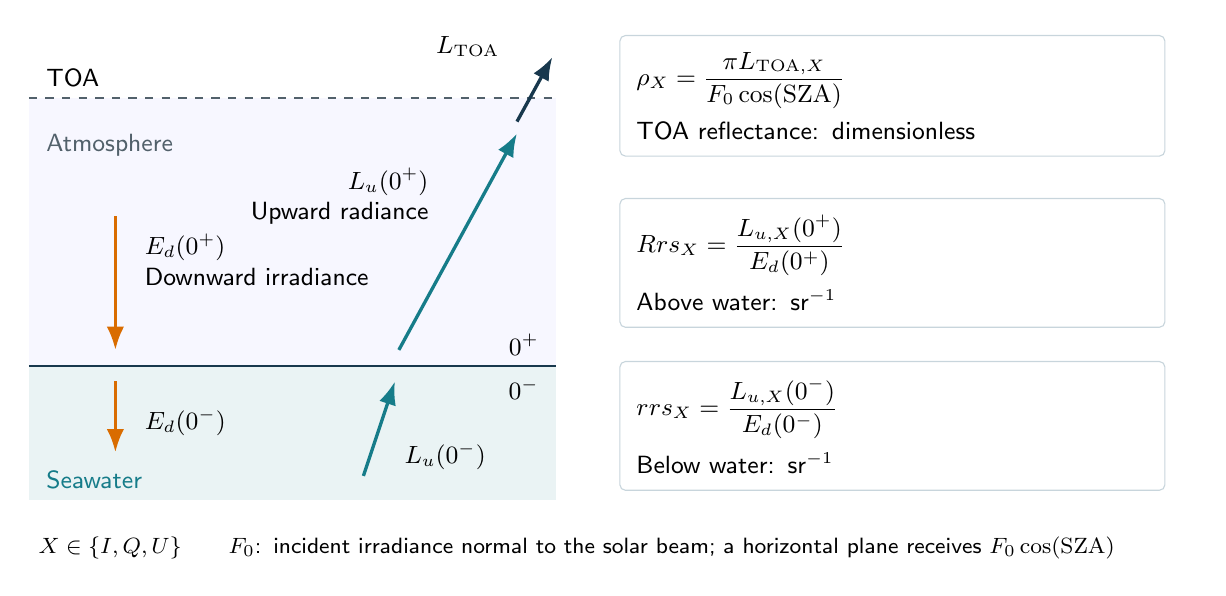
\begin{tikzpicture}[x=1cm,y=1cm,>=Latex,
 every node/.style={font=\sffamily\fontsize{9}{11}\selectfont},
 quantity/.style={draw=ocrtLine,rounded corners=2pt,fill=white,text width=6.5cm,align=left,inner sep=6pt}]
\fill[ocrtTeal!9] (0,0) rectangle (6.7,1.7);
\fill[blue!3] (0,1.7) rectangle (6.7,5.1);
\draw[ocrtNavy,thick] (0,1.7)--(6.7,1.7);
\draw[ocrtGray,dashed] (0,5.1)--(6.7,5.1);
\node[anchor=west] at (0.1,5.35) {TOA};
\node[anchor=west,text=ocrtGray] at (0.1,4.5) {\FigLang{대기}{Atmosphere}};
\node[anchor=west,text=ocrtTeal] at (0.1,0.25) {\FigLang{해수}{Seawater}};
\node[anchor=east] at (6.6,1.97) {$0^+$};
\node[anchor=east] at (6.6,1.40) {$0^-$};
\draw[->,very thick,orange!85!black] (1.1,3.6)--(1.1,1.9);
\node[anchor=west,align=left] at (1.35,3.05) {$E_d(0^+)$\\\FigLang{하향 조도}{Downward irradiance}};
\draw[->,very thick,orange!85!black] (1.1,1.5)--(1.1,0.6);
\node[anchor=west] at (1.35,0.98) {$E_d(0^-)$};
\draw[->,very thick,ocrtTeal] (4.25,0.3)--(4.65,1.5);
\node[anchor=west] at (4.65,0.55) {$L_u(0^-)$};
\draw[->,very thick,ocrtTeal] (4.7,1.9)--(6.2,4.65);
\node[anchor=east,align=right] at (5.2,3.85) {$L_u(0^+)$\\\FigLang{상향 휘도}{Upward radiance}};
\draw[->,very thick,ocrtNavy] (6.2,4.8)--(6.65,5.62);
\node[anchor=east] at (6.1,5.75) {$L_{\rm TOA}$};
\node[quantity,anchor=north west] at (7.5,5.9)
 {$\displaystyle \rho_X=\frac{\pi L_{{\rm TOA},X}}{F_0\cos({\rm SZA})}$\\[4pt]
  \FigLang{TOA 반사도: 무차원}{TOA reflectance: dimensionless}};
\node[quantity,anchor=north west] at (7.5,3.83)
 {$\displaystyle Rrs_X=\frac{L_{u,X}(0^+)}{E_d(0^+)}$\\[4pt]
  \FigLang{수면 위: sr$^{-1}$}{Above water: sr$^{-1}$}};
\node[quantity,anchor=north west] at (7.5,1.76)
 {$\displaystyle rrs_X=\frac{L_{u,X}(0^-)}{E_d(0^-)}$\\[4pt]
  \FigLang{수면 아래: sr$^{-1}$}{Below water: sr$^{-1}$}};
\node[anchor=north west,text width=14.6cm,align=left,font=\sffamily\footnotesize] at (0,-0.35)
 {$X\in\{I,Q,U\}$\qquad
  \FigLang{$F_0$: 태양광에 수직인 면의 입사량; 수평면에서는 $F_0\cos({\rm SZA})$}{$F_0$: incident irradiance normal to the solar beam; a horizontal plane receives $F_0\cos({\rm SZA})$}};
\end{tikzpicture}
\caption{\FigLang{출력 위치와 정규화의 구분. $0^+$와 $0^-$는 수면을 사이에 둔 서로 다른 위치다. 대문자 \texttt{Rrs}와 소문자 \texttt{rrs}는 교환할 수 없고, 둘에 $\pi$를 곱해도 대기 경로를 포함한 TOA \texttt{rho}가 되지 않는다. 화살표는 물리량의 방향과 평가 위치를 설명하는 도식이며 모든 산란 경로를 그린 것은 아니다.}{Output levels and their normalizations. $0^+$ and $0^-$ are distinct positions on opposite sides of the interface. Uppercase \texttt{Rrs} and lowercase \texttt{rrs} are not interchangeable. Multiplying either by $\pi$ does not produce TOA \texttt{rho}, which includes the atmosphere. Arrows identify directions and sampling levels schematically; they do not enumerate every scattering path.}}
\label{fig:output-levels}
\end{figure}

\FloatBarrier
Let \texttt{F0} denote the TOA spectral incident flux on a plane perpendicular to the solar propagation direction, and let \texttt{mu\_\allowbreak{}s=\allowbreak{}cos(SZA)}. The incident flux on a horizontal plane is then \texttt{F0*mu\_\allowbreak{}s}.


\begin{ManualCode}
rho_X = pi * L_TOA_X / (F0 * mu_s)          X = I, Q, U
Rrs_X = Lu_X(0+) / Ed(0+)                  [sr^-1]
rrs_X = Lu_X(0-) / Ed(0-)                  [sr^-1]
BRF0plus_X  = pi * Rrs_X                   [dimensionless]
BRF0minus_X = pi * rrs_X                   [dimensionless]
\end{ManualCode}

The atmospheric SOS solver includes \texttt{F0=\allowbreak{}\ensuremath{\pi}} in its source normalization, so it converts internal TOA intensity using \texttt{rho=\allowbreak{}I\_\allowbreak{}TOA/\allowbreak{}mu\_\allowbreak{}s}. Do not multiply the output \texttt{rho} by \ensuremath{\pi} or \texttt{1/\allowbreak{}mu\_\allowbreak{}s} again.

The underwater quantities \texttt{Lu/\allowbreak{}Qu/\allowbreak{}Uu} and \texttt{Ed/\allowbreak{}Eu} have radiance and irradiance dimensions, respectively, but \textbf{they are not absolute radiometric values obtained by reading a solar spectrum for an actual date or sensor.} The incident-light scales in the current C source are:


{\TableFont
\begin{longtable}{@{}>{\raggedright\arraybackslash}p{\dimexpr 0.3400\linewidth-4.00pt\relax}>{\raggedright\arraybackslash}p{\dimexpr 0.6600\linewidth-4.00pt\relax}@{}}
\toprule
\textbf{Water calculation path} & \textbf{Internal \texttt{F\_\allowbreak{}sun}} \\
\midrule
\endfirsthead
\toprule
\textbf{Water calculation path} & \textbf{Internal \texttt{F\_\allowbreak{}sun}} \\
\midrule
\endhead
\bottomrule
\endfoot
Original pure-seawater path; path switched to pure seawater by setting all OCRT/CCRR constituents to 0 & \ensuremath{\pi} \\
OCRT/CCRR path with nonzero constituents & 1 \\
Direct IOP path & 1 \\
Dedicated CCRR reference comparison & 1 \\
\end{longtable}
}

Direct comparison of raw \texttt{Lu/\allowbreak{}Ed} values from different paths can therefore include normalization differences. \texttt{Rrs}, \texttt{rrs}, and \texttt{rho} are normalized by their respective incident fluxes. To scale raw water radiance and irradiance to an actual \texttt{F0\_\allowbreak{}actual}, identify the \texttt{F\_\allowbreak{}sun} used and apply the factor \texttt{F0\_\allowbreak{}actual/\allowbreak{}F\_\allowbreak{}sun} in consistent physical units. Recover absolute TOA radiance from normalized \texttt{rho} using \texttt{L\_\allowbreak{}TOA=\allowbreak{}rho*F0\_\allowbreak{}actual*cos(SZA)/\allowbreak{}\ensuremath{\pi}}. The historical CLI option \texttt{-\allowbreak{}-\allowbreak{}f-\allowbreak{}sun} has been removed.


{\TableFont
\begin{longtable}{@{}>{\raggedright\arraybackslash}p{\dimexpr 0.3400\linewidth-4.00pt\relax}>{\raggedright\arraybackslash}p{\dimexpr 0.6600\linewidth-4.00pt\relax}@{}}
\toprule
\textbf{Quantity} & \textbf{Units and interpretation} \\
\midrule
\endfirsthead
\toprule
\textbf{Quantity} & \textbf{Units and interpretation} \\
\midrule
\endhead
\bottomrule
\endfoot
\texttt{rho}, \texttt{BRF}, \texttt{omega}, AOD, \texttt{tau\_\allowbreak{}R}, \texttt{T\_\allowbreak{}*} & Dimensionless; directional reflectances and transfer ratios are not energy probabilities necessarily bounded by 0--1 \\
\texttt{Rrs}, \texttt{rrs} & sr\textsuperscript{-}\textsuperscript{1} \\
\texttt{Lu}, \texttt{Qu}, \texttt{Uu}, \texttt{TOA\_\allowbreak{}water\_\allowbreak{}signal\_\allowbreak{}I} & Spectral radiance at the incident-light scale above; W m\textsuperscript{-}\textsuperscript{2} sr\textsuperscript{-}\textsuperscript{1} nm\textsuperscript{-}\textsuperscript{1} when given an actual physical scale \\
\texttt{Ed}, \texttt{Eu} & Spectral irradiance at the incident-light scale above; W m\textsuperscript{-}\textsuperscript{2} nm\textsuperscript{-}\textsuperscript{1} when given an actual physical scale \\
\texttt{a}, \texttt{b}, \texttt{bb}, \texttt{Kd}, \texttt{Ku} & m\textsuperscript{-}\textsuperscript{1} \\
Geometry & Degrees; \texttt{mu\_\allowbreak{}view} is dimensionless because it is \texttt{cos(VZA)} \\
\texttt{wavelength\_\allowbreak{}nm}, \texttt{AOD\_\allowbreak{}ref\_\allowbreak{}nm} & nm \\
\texttt{wind\_\allowbreak{}speed\_\allowbreak{}ms} & m s\textsuperscript{-}\textsuperscript{1} \\
\end{longtable}
}

\section{Distinguishing sunglint from TOA components}
\label{sec:auto:05_output_formats:3}
Single-geometry output for \texttt{ocean} provides both a base TOA quantity with direct sunglint separated out and a TOA quantity with direct sunglint added. \texttt{X} denotes each of \texttt{I/\allowbreak{}Q/\allowbreak{}U}.


\begin{ManualCode}
TOA_rho_water_total_X = TOA_rho_water_direct_X + TOA_rho_water_sky_X
TOA_rho_X = TOA_rho_atm_X + TOA_rho_water_total_X
TOA_rho_glint_on_X = TOA_rho_X + TOA_rho_glint_direct_X
\end{ManualCode}


{\TableFont
\begin{longtable}{@{}>{\raggedright\arraybackslash}p{\dimexpr 0.3400\linewidth-4.00pt\relax}>{\raggedright\arraybackslash}p{\dimexpr 0.6600\linewidth-4.00pt\relax}@{}}
\toprule
\textbf{Column or key} & \textbf{Meaning} \\
\midrule
\endfirsthead
\toprule
\textbf{Column or key} & \textbf{Meaning} \\
\midrule
\endhead
\bottomrule
\endfoot
\texttt{TOA\_\allowbreak{}rho\_\allowbreak{}atm\_\allowbreak{}I/\allowbreak{}Q/\allowbreak{}U} & Component calculated through a separate atmosphere--surface path in the coupled calculation; does not mean pure Rayleigh alone \\
\texttt{TOA\_\allowbreak{}rho\_\allowbreak{}water\_\allowbreak{}direct\_\allowbreak{}I/\allowbreak{}Q/\allowbreak{}U} & Underwater signal originating from direct sunlight, emerging through the surface and propagating through the atmosphere to TOA \\
\texttt{TOA\_\allowbreak{}rho\_\allowbreak{}water\_\allowbreak{}sky\_\allowbreak{}I/\allowbreak{}Q/\allowbreak{}U} & TOA component of the underwater signal originating from atmospheric downward diffuse light \\
\texttt{TOA\_\allowbreak{}rho\_\allowbreak{}water\_\allowbreak{}total\_\allowbreak{}I/\allowbreak{}Q/\allowbreak{}U} & Sum of the two water-origin components above \\
\texttt{TOA\_\allowbreak{}rho\_\allowbreak{}glint\_\allowbreak{}direct\_\allowbreak{}I/\allowbreak{}Q/\allowbreak{}U} & Direct-sunlight specular-reflection term at the water surface \\
\texttt{TOA\_\allowbreak{}rho\_\allowbreak{}glint\_\allowbreak{}on\_\allowbreak{}I/\allowbreak{}Q/\allowbreak{}U} & Base TOA plus direct sunglint \\
\end{longtable}
}

The word direct in \texttt{water\_\allowbreak{}direct} describes the \textbf{origin of the incident light}. It does not mean that the water signal has never scattered underwater or in the atmosphere. In contrast, direct in \texttt{Ed0plus\_\allowbreak{}direct} and \texttt{Ed0minus\_\allowbreak{}direct} below means \textbf{the unscattered parallel solar beam at that location}.

The ocean grid CSV columns \texttt{TOA\_\allowbreak{}rho\_\allowbreak{}I/\allowbreak{}Q/\allowbreak{}U} also represent this base ocean TOA. However, the current grid writer does not write \texttt{TOA\_\allowbreak{}rho\_\allowbreak{}glint\_\allowbreak{}on\_\allowbreak{}*} or the TOA decomposition columns above. For simulated datasets requiring these components, collect the named keys from single-geometry output.

For non-ocean \texttt{black\_\allowbreak{}fresnel\_\allowbreak{}ocean}, whether \texttt{rho\_\allowbreak{}I/\allowbreak{}Q/\allowbreak{}U} includes direct sunglint depends on \texttt{-\allowbreak{}-\allowbreak{}decouple-\allowbreak{}sunglint}. Do not confuse this with the corresponding ocean CSV \texttt{rho} definition. Specular reflection from a perfectly flat surface at wind speed 0 differs from finite-width Cox--Munk glint; a value at the exact specular direction cannot be interpreted in the same way as a case with wind.

\textbf{Caution about current non-ocean U diagnostics:} \texttt{rt\_\allowbreak{}solver.\allowbreak{}c} adds direct glint as \texttt{-U\_\allowbreak{}kernel} to the non-ocean total but records \texttt{+U\_\allowbreak{}kernel} in non-ocean \texttt{TOA\_\allowbreak{}rho\_\allowbreak{}glint\_\allowbreak{}direct\_\allowbreak{}U}. For \texttt{ocean}, the same-named key has the sign actually added to the total. Therefore, do not obtain glint-free U by directly subtracting the non-ocean diagnostic key from the total. Verify non-ocean polarization separation using a run with \texttt{-\allowbreak{}-\allowbreak{}decouple-\allowbreak{}sunglint}. This document records the output-sign inconsistency; it does not modify the code.

\section{Single-geometry text}
\label{sec:auto:05_output_formats:4}
The format is shown below. This is a format example, not a numerical prediction.


\begin{ManualCode}
<rho_I> <rho_Q> <rho_U>  TOA_rho_I=<value> ... sza=<value> vza=<value> raa=<value> wl=<value> orders=<integer> conv=<0-or-1>
\end{ManualCode}

The first three numbers equal the named \texttt{TOA\_\allowbreak{}rho\_\allowbreak{}I/\allowbreak{}Q/\allowbreak{}U} values. New analysis code should parse \texttt{key=\allowbreak{}value} entries instead of positional indices. \texttt{-\allowbreak{}-\allowbreak{}output-\allowbreak{}advanced} adds columns to batch CSV output; it does not change this single-geometry format.

\subsection{Keys common to all surfaces}
\label{sec:auto:05_output_formats:4.1}

{\TableFont
\begin{longtable}{@{}>{\raggedright\arraybackslash}p{\dimexpr 0.3400\linewidth-4.00pt\relax}>{\raggedright\arraybackslash}p{\dimexpr 0.6600\linewidth-4.00pt\relax}@{}}
\toprule
\textbf{Key} & \textbf{Meaning} \\
\midrule
\endfirsthead
\toprule
\textbf{Key} & \textbf{Meaning} \\
\midrule
\endhead
\bottomrule
\endfoot
\texttt{TOA\_\allowbreak{}rho\_\allowbreak{}I}, \texttt{TOA\_\allowbreak{}rho\_\allowbreak{}Q}, \texttt{TOA\_\allowbreak{}rho\_\allowbreak{}U} & TOA directional Stokes reflectance; see Section~\ref{sec:auto:05_output_formats:3} for glint inclusion \\
\texttt{TOA\_\allowbreak{}rho\_\allowbreak{}glint\_\allowbreak{}direct\_\allowbreak{}I/\allowbreak{}Q/\allowbreak{}U} & Direct-sunglint diagnostic; observe the non-ocean U-sign caution \\
\texttt{T\_\allowbreak{}dir\_\allowbreak{}dn}, \texttt{T\_\allowbreak{}diff\_\allowbreak{}dn\_\allowbreak{}hemi}, \texttt{T\_\allowbreak{}total\_\allowbreak{}dn\_\allowbreak{}hemi}, \texttt{T\_\allowbreak{}diff\_\allowbreak{}dn\_\allowbreak{}dir} & Downward transmittance definitions below \\
\texttt{T\_\allowbreak{}dir\_\allowbreak{}up\_\allowbreak{}view}, \texttt{T\_\allowbreak{}diff\_\allowbreak{}up\_\allowbreak{}view}, \texttt{T\_\allowbreak{}total\_\allowbreak{}up\_\allowbreak{}view} & Upward transmittance definitions below \\
\texttt{TOA\_\allowbreak{}water\_\allowbreak{}signal\_\allowbreak{}I}, \texttt{T\_\allowbreak{}up\_\allowbreak{}rt\_\allowbreak{}valid} & Water-origin TOA radiance and validity of the upward-transfer calculation \\
\texttt{AOD\_\allowbreak{}ref} & Aerosol optical depth at the specified reference wavelength \\
\texttt{AOD\_\allowbreak{}ref\_\allowbreak{}nm} & AOD reference wavelength, 555 or 865 nm \\
\texttt{AOD\_\allowbreak{}band} & AOD at the execution wavelength, calculated using the \texttt{.\allowbreak{}mie} extinction ratio \\
\texttt{AOD\_\allowbreak{}ext\_\allowbreak{}ratio} & Extinction at the execution wavelength divided by extinction at the reference wavelength; \texttt{AOD\_\allowbreak{}band=\allowbreak{}AOD\_\allowbreak{}ref*AOD\_\allowbreak{}ext\_\allowbreak{}ratio} \\
\texttt{sza}, \texttt{vza}, \texttt{raa}, \texttt{wl} & Execution geometry and wavelength; RAA follows the OCRT convention \\
\texttt{orders} & Non-ocean: maximum SOS order used across atmospheric Fourier modes; ocean: maximum order used by the underwater solution \\
\texttt{conv} & Non-ocean: logical AND of atmospheric-mode convergence; ocean: the underwater solution's \texttt{all\_\allowbreak{}converged} value \\
\end{longtable}
}

\texttt{conv=\allowbreak{}1} means that the applicable convergence criterion in the code was met. It does not establish spatial or angular grid independence, accuracy against other models, or independent validation of every atmospheric and underwater path in the full ocean calculation.

\subsection{Additional non-ocean keys}
\label{sec:auto:05_output_formats:4.2}

{\TableFont
\begin{longtable}{@{}>{\raggedright\arraybackslash}p{\dimexpr 0.3400\linewidth-4.00pt\relax}>{\raggedright\arraybackslash}p{\dimexpr 0.6600\linewidth-4.00pt\relax}@{}}
\toprule
\textbf{Key} & \textbf{Meaning} \\
\midrule
\endfirsthead
\toprule
\textbf{Key} & \textbf{Meaning} \\
\midrule
\endhead
\bottomrule
\endfoot
\texttt{tau\_\allowbreak{}R} & Total vertical Rayleigh optical depth used in the calculation \\
\texttt{diag\_\allowbreak{}sunglint\_\allowbreak{}up\_\allowbreak{}flux\_\allowbreak{}ratio} & Direct-glint diagnostic \texttt{rho\_\allowbreak{}I*cos(SZA)} \\
\texttt{diag\_\allowbreak{}TOA\_\allowbreak{}up\_\allowbreak{}flux\_\allowbreak{}ratio} & Base-TOA diagnostic \texttt{rho\_\allowbreak{}I*cos(SZA)} \\
\end{longtable}
}

Non-ocean calculations do not separately propagate an upward source supplied from the water. It is therefore normal for \texttt{T\_\allowbreak{}diff\_\allowbreak{}up\_\allowbreak{}view}, \texttt{T\_\allowbreak{}total\_\allowbreak{}up\_\allowbreak{}view}, and \texttt{TOA\_\allowbreak{}water\_\allowbreak{}signal\_\allowbreak{}I} to be \texttt{nan}, with \texttt{T\_\allowbreak{}up\_\allowbreak{}rt\_\allowbreak{}valid=\allowbreak{}0}.

\subsection{Additional ocean keys}
\label{sec:auto:05_output_formats:4.3}

{\TableFont
\begin{longtable}{@{}>{\raggedright\arraybackslash}p{\dimexpr 0.3400\linewidth-4.00pt\relax}>{\raggedright\arraybackslash}p{\dimexpr 0.6600\linewidth-4.00pt\relax}@{}}
\toprule
\textbf{Key} & \textbf{Meaning} \\
\midrule
\endfirsthead
\toprule
\textbf{Key} & \textbf{Meaning} \\
\midrule
\endhead
\bottomrule
\endfoot
\texttt{TOA\_\allowbreak{}rho\_\allowbreak{}atm\_\allowbreak{}I/\allowbreak{}Q/\allowbreak{}U}, \texttt{TOA\_\allowbreak{}rho\_\allowbreak{}water\_\allowbreak{}direct\_\allowbreak{}I/\allowbreak{}Q/\allowbreak{}U}, \texttt{TOA\_\allowbreak{}rho\_\allowbreak{}water\_\allowbreak{}sky\_\allowbreak{}I/\allowbreak{}Q/\allowbreak{}U}, \texttt{TOA\_\allowbreak{}rho\_\allowbreak{}water\_\allowbreak{}total\_\allowbreak{}I/\allowbreak{}Q/\allowbreak{}U}, \texttt{TOA\_\allowbreak{}rho\_\allowbreak{}glint\_\allowbreak{}on\_\allowbreak{}I/\allowbreak{}Q/\allowbreak{}U} & TOA decomposition in Section~\ref{sec:auto:05_output_formats:3} \\
\texttt{Lu0plus}, \texttt{Qu0plus}, \texttt{Uu0plus} & Water-origin Stokes radiance emerging into air at the surface \\
\texttt{Ed0plus} & Total downward irradiance on the air side of the surface \\
\texttt{Ed0plus\_\allowbreak{}direct}, \texttt{Ed0plus\_\allowbreak{}diffuse} & Decomposition of that irradiance into unscattered sunlight and the remaining hemispherically integrated contribution \\
\texttt{Rrs0plus\_\allowbreak{}I}, \texttt{Rrs0plus\_\allowbreak{}Q}, \texttt{Rrs0plus\_\allowbreak{}U} & The above radiances divided by \texttt{Ed0plus} \\
\texttt{BRF0plus\_\allowbreak{}I}, \texttt{BRF0plus\_\allowbreak{}Q}, \texttt{BRF0plus\_\allowbreak{}U} & \texttt{\ensuremath{\pi}*Rrs0plus\_\allowbreak{}X} for each component \\
\texttt{Lu0minus}, \texttt{Qu0minus}, \texttt{Uu0minus} & Upward Stokes radiance immediately below the surface \\
\texttt{Ed0minus}, \texttt{Eu0minus} & Total downward and upward irradiance immediately below the surface \\
\texttt{Ed0minus\_\allowbreak{}direct}, \texttt{Ed0minus\_\allowbreak{}diffuse} & Decomposition of underwater downward irradiance \\
\texttt{Eu0minus\_\allowbreak{}direct}, \texttt{Eu0minus\_\allowbreak{}diffuse} & Decomposition of underwater upward irradiance; in the current deep-water/black-bottom model, direct=0 and diffuse=Eu0minus \\
\texttt{rrs0minus\_\allowbreak{}I}, \texttt{rrs0minus\_\allowbreak{}Q}, \texttt{rrs0minus\_\allowbreak{}U} & Underwater upward Stokes radiance divided by \texttt{Ed0minus} \\
\texttt{BRF0minus\_\allowbreak{}I}, \texttt{BRF0minus\_\allowbreak{}Q}, \texttt{BRF0minus\_\allowbreak{}U} & \texttt{\ensuremath{\pi}*rrs0minus\_\allowbreak{}X} for each component \\
\texttt{Kd0minus}, \texttt{Ku0minus} & Near-surface logarithmic attenuation diagnostics for downward/upward irradiance, m\textsuperscript{-}\textsuperscript{1} \\
\texttt{a\_\allowbreak{}w}, \texttt{b\_\allowbreak{}w}, \texttt{bb\_\allowbreak{}w}, \texttt{a\_\allowbreak{}dom}, \texttt{a\_\allowbreak{}chl}, \texttt{a\_\allowbreak{}pig}, \texttt{b\_\allowbreak{}pig}, \texttt{bb\_\allowbreak{}pig}, \texttt{a\_\allowbreak{}min}, \texttt{b\_\allowbreak{}min}, \texttt{bb\_\allowbreak{}min}, \texttt{a\_\allowbreak{}total}, \texttt{b\_\allowbreak{}total}, \texttt{bb\_\allowbreak{}total}, \texttt{omega\_\allowbreak{}total} & IOP mapping in Section~\ref{sec:auto:05_output_formats:7} \\
\end{longtable}
}

\texttt{Kd/\allowbreak{}Ku} are near-surface diagnostics obtained from the finite difference \texttt{-ln(E(z1)/\allowbreak{}E(0))/\allowbreak{}z1} between the surface and the first calculation depth. In particular, \texttt{Ku} can be small or negative because of the near-surface irradiance gradient. Do not treat these as intrinsic attenuation coefficients constant at arbitrary depths or as validated satellite Kd products.

Ocean single-geometry output has no \texttt{tau\_\allowbreak{}R} key, and ocean grid output has no \texttt{Ku0minus}. Distinguish values present as internal object fields from values actually stored in public output files.

\section{Transmittance columns: what is divided by what?}
\label{sec:auto:05_output_formats:5}

{\TableFont
\begin{longtable}{@{}>{\raggedright\arraybackslash}p{\dimexpr 0.3400\linewidth-4.00pt\relax}>{\raggedright\arraybackslash}p{\dimexpr 0.6600\linewidth-4.00pt\relax}@{}}
\toprule
\textbf{Name} & \textbf{Definition and interpretation} \\
\midrule
\endfirsthead
\toprule
\textbf{Name} & \textbf{Definition and interpretation} \\
\midrule
\endhead
\bottomrule
\endfoot
\texttt{T\_\allowbreak{}dir\_\allowbreak{}dn} / \texttt{direct\_\allowbreak{}transmittance} & Attenuation of downward unscattered direct light. In plane-parallel geometry, \texttt{exp(-tau\_\allowbreak{}total/\allowbreak{}mu\_\allowbreak{}s)}; with IPSS, the corresponding spherical-path integral for direct light is applied \\
\texttt{T\_\allowbreak{}diff\_\allowbreak{}dn\_\allowbreak{}hemi} / \texttt{diffuse\_\allowbreak{}dn\_\allowbreak{}hemi} & Downward diffuse irradiance on the air side of the surface divided by TOA horizontal incident flux \\
\texttt{T\_\allowbreak{}total\_\allowbreak{}dn\_\allowbreak{}hemi} / \texttt{irradiance\_\allowbreak{}transmittance} & \texttt{T\_\allowbreak{}dir\_\allowbreak{}dn+T\_\allowbreak{}diff\_\allowbreak{}dn\_\allowbreak{}hemi}; total downward irradiance above the surface divided by TOA horizontal incident flux \\
\texttt{T\_\allowbreak{}diff\_\allowbreak{}dn\_\allowbreak{}dir} / \texttt{diffuse\_\allowbreak{}dn\_\allowbreak{}dir} & Directional diagnostic defined using downward diffuse radiance in the requested direction: \texttt{2*pi*mu\_\allowbreak{}v*L\_\allowbreak{}dn\_\allowbreak{}diff/\allowbreak{}(F0*mu\_\allowbreak{}s)} \\
\texttt{T\_\allowbreak{}dir\_\allowbreak{}up\_\allowbreak{}view} & Upward unscattered attenuation at the requested VZA, \texttt{exp(-tau\_\allowbreak{}total/\allowbreak{}mu\_\allowbreak{}v)} \\
\texttt{T\_\allowbreak{}total\_\allowbreak{}up\_\allowbreak{}view} & Result of transferring the actual angular distribution of water-leaving light through the atmosphere, \texttt{TOA\_\allowbreak{}water\_\allowbreak{}signal\_\allowbreak{}I/\allowbreak{}Lu(0+)} \\
\texttt{T\_\allowbreak{}diff\_\allowbreak{}up\_\allowbreak{}view} & \texttt{T\_\allowbreak{}total\_\allowbreak{}up\_\allowbreak{}view-T\_\allowbreak{}dir\_\allowbreak{}up\_\allowbreak{}view} \\
\texttt{TOA\_\allowbreak{}water\_\allowbreak{}signal\_\allowbreak{}I} & TOA radiance from the water signal alone; numerator of the upward transfer ratio \\
\texttt{T\_\allowbreak{}up\_\allowbreak{}rt\_\allowbreak{}valid} & 1 when the required atmospheric bottom-source SOS propagation of water-origin light has completed, or the atmosphere is absent, and the denominator is valid; otherwise 0 \\
\end{longtable}
}

\texttt{T\_\allowbreak{}diff\_\allowbreak{}dn\_\allowbreak{}dir} is not a hemispheric integral. Simply summing RAA samples does not produce \texttt{T\_\allowbreak{}diff\_\allowbreak{}dn\_\allowbreak{}hemi}; directions and integration weights must be included. \texttt{T\_\allowbreak{}total\_\allowbreak{}up\_\allowbreak{}view} depends on the scene's angular distribution of water-leaving light. Do not reuse it as an “atmosphere-only upward-transmittance LUT” independent of water IOPs and geometry. Do not automatically clip directional transfer ratios greater than 1.

When \texttt{T\_\allowbreak{}up\_\allowbreak{}rt\_\allowbreak{}valid=\allowbreak{}0}, do not apply corrections using the upward diffuse or total transfer ratio. Do not automatically substitute \texttt{T\_\allowbreak{}diff\_\allowbreak{}dn\_\allowbreak{}hemi} as an up/down symmetry approximation simply because a numerical value is needed.

The following quantities are not transmittances.


{\TableFont
\begin{longtable}{@{}>{\raggedright\arraybackslash}p{\dimexpr 0.3000\linewidth-5.33pt\relax}>{\raggedright\arraybackslash}p{\dimexpr 0.2300\linewidth-5.33pt\relax}>{\raggedright\arraybackslash}p{\dimexpr 0.4700\linewidth-5.33pt\relax}@{}}
\toprule
\textbf{LUT column} & \textbf{Single-geometry key} & \textbf{Definition} \\
\midrule
\endfirsthead
\toprule
\textbf{LUT column} & \textbf{Single-geometry key} & \textbf{Definition} \\
\midrule
\endhead
\bottomrule
\endfoot
\texttt{sunglint\_\allowbreak{}up\_\allowbreak{}flux\_\allowbreak{}ratio\_\allowbreak{}diag} & \texttt{diag\_\allowbreak{}sunglint\_\allowbreak{}up\_\allowbreak{}flux\_\allowbreak{}ratio} & \texttt{rho\_\allowbreak{}glint\_\allowbreak{}I*mu\_\allowbreak{}s} \\
\texttt{toa\_\allowbreak{}up\_\allowbreak{}flux\_\allowbreak{}ratio\_\allowbreak{}diag} & \texttt{diag\_\allowbreak{}TOA\_\allowbreak{}up\_\allowbreak{}flux\_\allowbreak{}ratio} & \texttt{rho\_\allowbreak{}TOA\_\allowbreak{}I*mu\_\allowbreak{}s} \\
\end{longtable}
}

Although their names contain flux, these are \textbf{legacy diagnostics based on directional radiance}, not integrals of upward flux over the full hemisphere. Do not interpret them as \texttt{T\_\allowbreak{}total\_\allowbreak{}up\_\allowbreak{}view}.

\section{Non-ocean LUT CSV: 13 columns}
\label{sec:auto:05_output_formats:6}
The actual header is:


\begin{ManualCode}
sza_deg,wavelength_nm,vza_deg,raa_deg,rho_I,rho_Q,rho_U,direct_transmittance,irradiance_transmittance,diffuse_dn_hemi,diffuse_dn_dir,sunglint_up_flux_ratio_diag,toa_up_flux_ratio_diag
\end{ManualCode}

The first four columns are coordinates; \texttt{rho\_\allowbreak{}I/\allowbreak{}Q/\allowbreak{}U} are TOA reflectances. The remaining columns follow the definitions in Section~\ref{sec:auto:05_output_formats:5}. \texttt{direct\_\allowbreak{}transmittance}, \texttt{irradiance\_\allowbreak{}transmittance}, and \texttt{diffuse\_\allowbreak{}dn\_\allowbreak{}hemi} are scalars repeated for every direction in a case with the same SZA, wavelength, atmosphere, and surface. \texttt{rho}, \texttt{diffuse\_\allowbreak{}dn\_\allowbreak{}dir}, and the two \texttt{*\_\allowbreak{}diag} quantities are directional values.

This CSV represents the atmospheric calculation on the \texttt{0+} side. It does not provide \texttt{Rrs}, \texttt{rrs}, water IOPs, or the validity of upward water-signal propagation. Interpreting \texttt{rho} also requires settings absent from the file: \texttt{surface}, \texttt{pressure}, AOD, \texttt{.\allowbreak{}mie}, absorption, and glint separation. Retain the execution command with the file.

\section{Ocean full-grid CSV}
\label{sec:auto:05_output_formats:7}
The actual header, in order, is:


\begin{ManualCode}
case_kind,sza_deg,wavelength_nm,wind_speed_ms,n_mu,mu_index,mu_view,vza_deg,raa_deg,Ed0plus_air,Ed0plus_direct,Ed0plus_diffuse,Lu0plus_I,Lu0plus_Q,Lu0plus_U,Rrs_I,Rrs_Q,Rrs_U,Ed0minus_water,Ed0minus_direct,Ed0minus_diffuse,Eu0minus_water,Eu0minus_direct,Eu0minus_diffuse,Lu0minus_I,Lu0minus_Q,Lu0minus_U,rrs_I,rrs_Q,rrs_U,TOA_rho_I,TOA_rho_Q,TOA_rho_U,T_dir_dn,T_diff_dn_hemi,T_total_dn_hemi,T_diff_dn_dir,T_dir_up_view,T_diff_up_view,T_total_up_view,TOA_water_signal_I,T_up_rt_valid,a_total,b_total,bb_total,omega_water,water_orders,water_converged,a_w,b_w,bb_w,a_chl,a_phyto_detritus,b_phyto_detritus,bb_phyto_detritus,a_dom,a_min,b_min,bb_min,Kd0minus
\end{ManualCode}

\subsection{Coordinates, identifiers, and convergence}
\label{sec:auto:05_output_formats:7.1}

{\TableFont
\begin{longtable}{@{}>{\raggedright\arraybackslash}p{\dimexpr 0.3400\linewidth-4.00pt\relax}>{\raggedright\arraybackslash}p{\dimexpr 0.6600\linewidth-4.00pt\relax}@{}}
\toprule
\textbf{Column} & \textbf{Meaning} \\
\midrule
\endfirsthead
\toprule
\textbf{Column} & \textbf{Meaning} \\
\midrule
\endhead
\bottomrule
\endfoot
\texttt{case\_\allowbreak{}kind} & Fixed string \texttt{ocean\_\allowbreak{}rrs\_\allowbreak{}grid} \\
\texttt{sza\_\allowbreak{}deg}, \texttt{wavelength\_\allowbreak{}nm}, \texttt{wind\_\allowbreak{}speed\_\allowbreak{}ms} & Case SZA, wavelength, and wind speed \\
\texttt{n\_\allowbreak{}mu} & Number of positive atmospheric Gauss integration nodes; not the number of output VZAs or underwater nodes \\
\texttt{mu\_\allowbreak{}index} & Zero-based group index for the output VZA; not a Gauss-node index \\
\texttt{mu\_\allowbreak{}view}, \texttt{vza\_\allowbreak{}deg}, \texttt{raa\_\allowbreak{}deg} & \texttt{cos(VZA)}, VZA in air, and OCRT RAA \\
\texttt{water\_\allowbreak{}orders}, \texttt{water\_\allowbreak{}converged} & Maximum underwater SOS order and underwater convergence flag \\
\end{longtable}
}

\subsection{Radiometric quantities, transmittance, and reflectance}
\label{sec:auto:05_output_formats:7.2}

{\TableFont
\begin{longtable}{@{}>{\raggedright\arraybackslash}p{\dimexpr 0.3400\linewidth-4.00pt\relax}>{\raggedright\arraybackslash}p{\dimexpr 0.6600\linewidth-4.00pt\relax}@{}}
\toprule
\textbf{Column} & \textbf{Corresponding single-geometry key or definition} \\
\midrule
\endfirsthead
\toprule
\textbf{Column} & \textbf{Corresponding single-geometry key or definition} \\
\midrule
\endhead
\bottomrule
\endfoot
\texttt{Ed0plus\_\allowbreak{}air} & \texttt{Ed0plus} \\
\texttt{Ed0plus\_\allowbreak{}direct}, \texttt{Ed0plus\_\allowbreak{}diffuse} & Same names; their sum is \texttt{Ed0plus\_\allowbreak{}air} \\
\texttt{Lu0plus\_\allowbreak{}I}, \texttt{Lu0plus\_\allowbreak{}Q}, \texttt{Lu0plus\_\allowbreak{}U} & \texttt{Lu0plus}, \texttt{Qu0plus}, \texttt{Uu0plus}, respectively \\
\texttt{Rrs\_\allowbreak{}I}, \texttt{Rrs\_\allowbreak{}Q}, \texttt{Rrs\_\allowbreak{}U} & \texttt{Rrs0plus\_\allowbreak{}I/\allowbreak{}Q/\allowbreak{}U}, respectively \\
\texttt{Ed0minus\_\allowbreak{}water} & \texttt{Ed0minus} \\
\texttt{Ed0minus\_\allowbreak{}direct}, \texttt{Ed0minus\_\allowbreak{}diffuse} & Same names; their sum is \texttt{Ed0minus\_\allowbreak{}water} \\
\texttt{Eu0minus\_\allowbreak{}water} & \texttt{Eu0minus} \\
\texttt{Eu0minus\_\allowbreak{}direct}, \texttt{Eu0minus\_\allowbreak{}diffuse} & Same names; their sum is \texttt{Eu0minus\_\allowbreak{}water} \\
\texttt{Lu0minus\_\allowbreak{}I}, \texttt{Lu0minus\_\allowbreak{}Q}, \texttt{Lu0minus\_\allowbreak{}U} & \texttt{Lu0minus}, \texttt{Qu0minus}, \texttt{Uu0minus}, respectively \\
\texttt{rrs\_\allowbreak{}I}, \texttt{rrs\_\allowbreak{}Q}, \texttt{rrs\_\allowbreak{}U} & \texttt{rrs0minus\_\allowbreak{}I/\allowbreak{}Q/\allowbreak{}U}, respectively \\
\texttt{TOA\_\allowbreak{}rho\_\allowbreak{}I}, \texttt{TOA\_\allowbreak{}rho\_\allowbreak{}Q}, \texttt{TOA\_\allowbreak{}rho\_\allowbreak{}U} & Base ocean TOA reflectance \\
\texttt{T\_\allowbreak{}dir\_\allowbreak{}dn}, \texttt{T\_\allowbreak{}diff\_\allowbreak{}dn\_\allowbreak{}hemi}, \texttt{T\_\allowbreak{}total\_\allowbreak{}dn\_\allowbreak{}hemi}, \texttt{T\_\allowbreak{}diff\_\allowbreak{}dn\_\allowbreak{}dir} & Downward transfer quantities in Section~\ref{sec:auto:05_output_formats:5} \\
\texttt{T\_\allowbreak{}dir\_\allowbreak{}up\_\allowbreak{}view}, \texttt{T\_\allowbreak{}diff\_\allowbreak{}up\_\allowbreak{}view}, \texttt{T\_\allowbreak{}total\_\allowbreak{}up\_\allowbreak{}view} & Upward transfer quantities in Section~\ref{sec:auto:05_output_formats:5} \\
\texttt{TOA\_\allowbreak{}water\_\allowbreak{}signal\_\allowbreak{}I}, \texttt{T\_\allowbreak{}up\_\allowbreak{}rt\_\allowbreak{}valid} & Upward water signal and validity in Section~\ref{sec:auto:05_output_formats:5} \\
\texttt{Kd0minus} & Near-surface downward-irradiance attenuation diagnostic \\
\end{longtable}
}

\subsection{IOP metadata}
\label{sec:auto:05_output_formats:7.3}
These coefficients are the values \textbf{actually used} in the calculation. In direct IOP input mode, do not infer a biological decomposition from component values. Use \texttt{a\_\allowbreak{}total}, \texttt{b\_\allowbreak{}total}, and \texttt{bb\_\allowbreak{}total} for totals.


{\TableFont
\begin{longtable}{@{}>{\raggedright\arraybackslash}p{\dimexpr 0.3000\linewidth-5.33pt\relax}>{\raggedright\arraybackslash}p{\dimexpr 0.2300\linewidth-5.33pt\relax}>{\raggedright\arraybackslash}p{\dimexpr 0.4700\linewidth-5.33pt\relax}@{}}
\toprule
\textbf{Grid column} & \textbf{Single-geometry key} & \textbf{Meaning} \\
\midrule
\endfirsthead
\toprule
\textbf{Grid column} & \textbf{Single-geometry key} & \textbf{Meaning} \\
\midrule
\endhead
\bottomrule
\endfoot
\texttt{a\_\allowbreak{}total}, \texttt{b\_\allowbreak{}total}, \texttt{bb\_\allowbreak{}total} & Same & Total absorption, scattering, and backscattering, m\textsuperscript{-}\textsuperscript{1} \\
\texttt{omega\_\allowbreak{}water} & \texttt{omega\_\allowbreak{}total} & Underwater single-scattering albedo \texttt{b\_\allowbreak{}total/\allowbreak{}(a\_\allowbreak{}total+b\_\allowbreak{}total)} \\
\texttt{a\_\allowbreak{}w}, \texttt{b\_\allowbreak{}w}, \texttt{bb\_\allowbreak{}w} & Same & Pure-seawater components \\
\texttt{a\_\allowbreak{}chl} & Same & Phytoplankton absorption component alone; not chlorophyll concentration itself \\
\texttt{a\_\allowbreak{}phyto\_\allowbreak{}detritus}, \texttt{b\_\allowbreak{}phyto\_\allowbreak{}detritus}, \texttt{bb\_\allowbreak{}phyto\_\allowbreak{}detritus} & \texttt{a\_\allowbreak{}pig}, \texttt{b\_\allowbreak{}pig}, \texttt{bb\_\allowbreak{}pig} & Phytoplankton and organic detrital particle components used in the code \\
\texttt{a\_\allowbreak{}dom} & Same & Dissolved-organic-matter absorption component \\
\texttt{a\_\allowbreak{}min}, \texttt{b\_\allowbreak{}min}, \texttt{bb\_\allowbreak{}min} & Same & Mineral-particle components \\
\end{longtable}
}

\texttt{a\_\allowbreak{}chl} is the phytoplankton-absorption portion of \texttt{a\_\allowbreak{}phyto\_\allowbreak{}detritus}; do not add both again as independent components when summing total absorption. Component pathways differ between models, so validate against the reported totals rather than reconstructed sums.

\section{Specified-geometry batch CSV}
\label{sec:auto:05_output_formats:8}
The current basic header is:


\begin{ManualCode}
case_id,sza_deg,vza_deg,raa_deg,wavelength_nm,rho_I_v2,rho_Q_v2,rho_U_v2
\end{ManualCode}

For the nine-column aerosol input layout, \texttt{aod\_\allowbreak{}ref} is inserted after \texttt{wavelength\_\allowbreak{}nm}. This is AOD at the reference wavelength, not at the execution wavelength. Retain the input header and command to record whether the reference wavelength is 555 or 865. \texttt{\_\allowbreak{}v2} is a column-name suffix retained for compatibility with existing files; it is not a separate physical definition or executable version number.

With \texttt{-\allowbreak{}-\allowbreak{}output-\allowbreak{}advanced}, the following columns follow the coordinates:


\begin{ManualCode}
rho_I_v2,rho_I_ref,delta_abs,delta_rel_pct,delta_rel_abs_pct,tau_R_v2,tau_R_ref,n_orders_m0,n_orders_m1,n_orders_m2,walltime_ms
\end{ManualCode}

If reference Q/U values are absent, \texttt{rho\_\allowbreak{}Q\_\allowbreak{}v2,\allowbreak{}rho\_\allowbreak{}U\_\allowbreak{}v2} are appended. If both reference Q and U are present, the following columns are appended instead:


\begin{ManualCode}
rho_Q_v2,rho_Q_ref,delta_abs_Q,delta_rel_pct_Q,delta_rel_abs_pct_Q,rho_U_v2,rho_U_ref,delta_abs_U,delta_rel_pct_U,delta_rel_abs_pct_U
\end{ManualCode}


{\TableFont
\begin{longtable}{@{}>{\raggedright\arraybackslash}p{\dimexpr 0.3400\linewidth-4.00pt\relax}>{\raggedright\arraybackslash}p{\dimexpr 0.6600\linewidth-4.00pt\relax}@{}}
\toprule
\textbf{Column} & \textbf{Definition and caution} \\
\midrule
\endfirsthead
\toprule
\textbf{Column} & \textbf{Definition and caution} \\
\midrule
\endhead
\bottomrule
\endfoot
\texttt{case\_\allowbreak{}id} & Input integer identifier; also used in per-row grid filenames \\
\texttt{rho\_\allowbreak{}I\_\allowbreak{}v2}, \texttt{rho\_\allowbreak{}Q\_\allowbreak{}v2}, \texttt{rho\_\allowbreak{}U\_\allowbreak{}v2} & Calculated TOA reflectance \\
\texttt{rho\_\allowbreak{}I\_\allowbreak{}ref}, \texttt{rho\_\allowbreak{}Q\_\allowbreak{}ref}, \texttt{rho\_\allowbreak{}U\_\allowbreak{}ref} & Input reference reflectance \\
\texttt{delta\_\allowbreak{}abs} & \texttt{rho\_\allowbreak{}I\_\allowbreak{}v2-rho\_\allowbreak{}I\_\allowbreak{}ref}; despite abs in its name, this is a \textbf{signed difference} \\
\texttt{delta\_\allowbreak{}rel\_\allowbreak{}pct} & \texttt{100*(rho\_\allowbreak{}I\_\allowbreak{}v2-rho\_\allowbreak{}I\_\allowbreak{}ref)/\allowbreak{}rho\_\allowbreak{}I\_\allowbreak{}ref} \\
\texttt{delta\_\allowbreak{}rel\_\allowbreak{}abs\_\allowbreak{}pct} & \texttt{abs(delta\_\allowbreak{}rel\_\allowbreak{}pct)} \\
\texttt{delta\_\allowbreak{}abs\_\allowbreak{}Q}, \texttt{delta\_\allowbreak{}abs\_\allowbreak{}U} & Calculated Q/U minus reference Q/U, respectively; signed differences \\
\texttt{delta\_\allowbreak{}rel\_\allowbreak{}pct\_\allowbreak{}Q}, \texttt{delta\_\allowbreak{}rel\_\allowbreak{}pct\_\allowbreak{}U} & \texttt{100*delta\_\allowbreak{}Q\_\allowbreak{}or\_\allowbreak{}U/\allowbreak{}abs(rho\_\allowbreak{}I\_\allowbreak{}ref)}; the denominator is \textbf{the absolute value of reference I}, not the Q/U reference \\
\texttt{delta\_\allowbreak{}rel\_\allowbreak{}abs\_\allowbreak{}pct\_\allowbreak{}Q}, \texttt{delta\_\allowbreak{}rel\_\allowbreak{}abs\_\allowbreak{}pct\_\allowbreak{}U} & Absolute values of the percentage differences above \\
\texttt{tau\_\allowbreak{}R\_\allowbreak{}v2}, \texttt{tau\_\allowbreak{}R\_\allowbreak{}ref} & Calculated and input Rayleigh optical depths \\
\texttt{n\_\allowbreak{}orders\_\allowbreak{}m0}, \texttt{n\_\allowbreak{}orders\_\allowbreak{}m1}, \texttt{n\_\allowbreak{}orders\_\allowbreak{}m2} & SOS orders recorded only for Fourier modes 0/1/2; do not represent the maximum order of higher modes \\
\texttt{walltime\_\allowbreak{}ms} & Elapsed time for the row calculation and associated processing, in milliseconds; the simple sum does not equal total parallel-batch time \\
\end{longtable}
}

If reference I is absent, reference and error columns are empty. If reference I is 0, this batch writer records relative error as 0. Do not interpret this as “no error”; reclassify it as undefined relative error. Failed-row return codes have no separate CSV column, so also check the process exit code, stderr, and finiteness of the values.

This \texttt{-\allowbreak{}-\allowbreak{}batch} is the atmospheric specified-geometry path in \texttt{rt\_\allowbreak{}io\_\allowbreak{}run\_\allowbreak{}batch()}. Do not use it as a general batch interface for ocean constituents or IOPs. In current \texttt{main.\allowbreak{}c}, this path returns before gas-absorption initialization, so gas options are not actually applied. Case-template copying is also limited: this is not a path that passes every CLI setting, such as continuous atmospheric-pressure values, to each row. For scientific LUTs varying gas and pressure, repeat single-case grid runs. For ocean work, use \texttt{-\allowbreak{}-\allowbreak{}batch-\allowbreak{}full-\allowbreak{}grid} or repeated single-geometry runs.

When \texttt{case\_\allowbreak{}<id>.\allowbreak{}csv} files are also written, their contents use the non-ocean 13-column format in Section~\ref{sec:auto:05_output_formats:6}. Repeated \texttt{case\_\allowbreak{}id} values produce the same filename, so make input identifiers unique. Failure to open a per-row LUT file may not be fully reflected in the summary success status; also check file counts and row counts.

\section{CCRR comparison CSV}
\label{sec:auto:05_output_formats:9}
This format is intended for reference comparisons rather than general production simulations. The header consists of the following groups; names within each group are the actual column names.


{\TableFont
\begin{longtable}{@{}>{\raggedright\arraybackslash}p{\dimexpr 0.3400\linewidth-4.00pt\relax}>{\raggedright\arraybackslash}p{\dimexpr 0.6600\linewidth-4.00pt\relax}@{}}
\toprule
\textbf{Column group} & \textbf{Definition} \\
\midrule
\endfirsthead
\toprule
\textbf{Column group} & \textbf{Definition} \\
\midrule
\endhead
\bottomrule
\endfoot
\texttt{case\_\allowbreak{}id,\allowbreak{}wavelength\_\allowbreak{}nm,\allowbreak{}chl\_\allowbreak{}mg\_\allowbreak{}m3,\allowbreak{}min\_\allowbreak{}g\_\allowbreak{}m3,\allowbreak{}adom\_\allowbreak{}440\_\allowbreak{}m-\allowbreak{}1,\allowbreak{}adom\_\allowbreak{}s\_\allowbreak{}nm-\allowbreak{}1} & Input case ID, wavelength, Chl (mg m\textsuperscript{-}\textsuperscript{3}), mineral concentration (g m\textsuperscript{-}\textsuperscript{3}), organic-matter absorption at 440 nm (m\textsuperscript{-}\textsuperscript{1}), and spectral slope (nm\textsuperscript{-}\textsuperscript{1}) \\
\texttt{sza\_\allowbreak{}air\_\allowbreak{}deg,\allowbreak{}vza\_\allowbreak{}air\_\allowbreak{}deg,\allowbreak{}raa\_\allowbreak{}ccrr\_\allowbreak{}deg,\allowbreak{}raa\_\allowbreak{}ocrt\_\allowbreak{}deg,\allowbreak{}raa\_\allowbreak{}mapping} & Geometry in air and RAA before/after conversion; mapping string is \texttt{180-\allowbreak{}minus-\allowbreak{}ccrr} \\
\texttt{wind\_\allowbreak{}speed\_\allowbreak{}ms,\allowbreak{}sunglint\_\allowbreak{}decoupled} & Wind speed 0 and glint separation 1, fixed by the comparison path \\
\texttt{OCRT\_\allowbreak{}Ed0minus,\allowbreak{}OCRT\_\allowbreak{}Lu0minus,\allowbreak{}OCRT\_\allowbreak{}rrs,\allowbreak{}OCRT\_\allowbreak{}Ed0plus,\allowbreak{}OCRT\_\allowbreak{}Lu0plus\_\allowbreak{}no\_\allowbreak{}sky,\allowbreak{}OCRT\_\allowbreak{}Rrs} & Calculated irradiance, radiance, and reflectance \\
\texttt{OCRT\_\allowbreak{}a\_\allowbreak{}total,\allowbreak{}OCRT\_\allowbreak{}b\_\allowbreak{}total,\allowbreak{}OCRT\_\allowbreak{}bb\_\allowbreak{}total} & Calculated total IOPs \\
\texttt{OCRT\_\allowbreak{}a\_\allowbreak{}w,\allowbreak{}OCRT\_\allowbreak{}b\_\allowbreak{}w,\allowbreak{}OCRT\_\allowbreak{}bb\_\allowbreak{}w,\allowbreak{}OCRT\_\allowbreak{}a\_\allowbreak{}dom,\allowbreak{}OCRT\_\allowbreak{}a\_\allowbreak{}pig,\allowbreak{}OCRT\_\allowbreak{}b\_\allowbreak{}pig,\allowbreak{}OCRT\_\allowbreak{}bb\_\allowbreak{}pig,\allowbreak{}OCRT\_\allowbreak{}a\_\allowbreak{}min,\allowbreak{}OCRT\_\allowbreak{}b\_\allowbreak{}min,\allowbreak{}OCRT\_\allowbreak{}bb\_\allowbreak{}min} & Calculated component IOPs; same meanings as in Section~\ref{sec:auto:05_output_formats:7} \\
\texttt{OCRT\_\allowbreak{}orders,\allowbreak{}OCRT\_\allowbreak{}conv} & Underwater order and convergence flag \\
\texttt{ref\_\allowbreak{}Ed0minus,\allowbreak{}ref\_\allowbreak{}Lu0minus,\allowbreak{}ref\_\allowbreak{}rrs,\allowbreak{}ref\_\allowbreak{}Ed0plus,\allowbreak{}ref\_\allowbreak{}Lu0plus\_\allowbreak{}no\_\allowbreak{}sky,\allowbreak{}ref\_\allowbreak{}Rrs,\allowbreak{}ref\_\allowbreak{}a\_\allowbreak{}total,\allowbreak{}ref\_\allowbreak{}b\_\allowbreak{}total,\allowbreak{}ref\_\allowbreak{}bb\_\allowbreak{}total} & Corresponding reference values from the input file \\
\texttt{rel\_\allowbreak{}Ed0minus\_\allowbreak{}pct,\allowbreak{}rel\_\allowbreak{}Lu0minus\_\allowbreak{}pct,\allowbreak{}rel\_\allowbreak{}rrs\_\allowbreak{}pct,\allowbreak{}rel\_\allowbreak{}Ed0plus\_\allowbreak{}pct,\allowbreak{}rel\_\allowbreak{}Lu0plus\_\allowbreak{}no\_\allowbreak{}sky\_\allowbreak{}pct,\allowbreak{}rel\_\allowbreak{}Rrs\_\allowbreak{}pct,\allowbreak{}rel\_\allowbreak{}a\_\allowbreak{}total\_\allowbreak{}pct,\allowbreak{}rel\_\allowbreak{}b\_\allowbreak{}total\_\allowbreak{}pct,\allowbreak{}rel\_\allowbreak{}bb\_\allowbreak{}total\_\allowbreak{}pct} & \texttt{100*(OCRT/\allowbreak{}ref-1)} for each quantity; \texttt{nan} if the reference is missing, 0, or nonfinite \\
\end{longtable}
}

\texttt{OCRT\_\allowbreak{}Lu0plus\_\allowbreak{}no\_\allowbreak{}sky} actually records \texttt{res.\allowbreak{}Lu\_\allowbreak{}0plus\_\allowbreak{}view}. Do not infer from the column name alone that it also excludes the contribution created by atmospheric downward diffuse light entering the water. Match the reference definition of \texttt{no\_\allowbreak{}sky}: it may mean exclusion of surface-reflected skylight, or it may additionally exclude diffuse light incident into the water.

This comparison path fixes \texttt{F\_\allowbreak{}sun=\allowbreak{}1}. Check that reference \texttt{Lu/\allowbreak{}Ed} values use the same incident-flux normalization. This path also runs before general gas-absorption initialization; do not treat it as a general-purpose validation batch that includes gas options.

\section{Minimum metadata for saved datasets}
\label{sec:auto:05_output_formats:10}
The basic CSV alone cannot reconstruct all execution conditions. Retain the following with LUTs and simulated training data:

\begin{itemize}
\item Git commit and executable identifier, execution command, and environment variables used.
\item RAA definition and SAA/VAA conversion formulas, whether 0--360\textdegree{} is preserved, the Stokes reference plane, and U-sign handling.
\item Surface mode, glint separation, water model, and all constituent/IOP inputs.
\item Wavelength, atmospheric pressure, AOD reference wavelength and value, aerosol \texttt{.\allowbreak{}mie}, gas-absorption conditions, water temperature, salinity, and wind speed.
\item Optical LUT and phase-function files used, numerical settings, exit code, and error logs.
\item For raw \texttt{Lu/\allowbreak{}Ed}, the internal \texttt{F\_\allowbreak{}sun} scale and whether conversion to actual incident light was applied.
\end{itemize}

For each sample, you can check \texttt{Rrs=\allowbreak{}Lu0plus\_\allowbreak{}I/\allowbreak{}Ed0plus\_\allowbreak{}air}, \texttt{rrs=\allowbreak{}Lu0minus\_\allowbreak{}I/\allowbreak{}Ed0minus\_\allowbreak{}water}, \texttt{T\_\allowbreak{}total\_\allowbreak{}dn\_\allowbreak{}hemi=\allowbreak{}T\_\allowbreak{}dir\_\allowbreak{}dn+T\_\allowbreak{}diff\_\allowbreak{}dn\_\allowbreak{}hemi}, and each direct+diffuse irradiance sum. These internal-consistency checks do not validate the RAA convention or accuracy against an external reference.

\subsection{Implementation references}
\label{sec:auto:05_output_formats:10.1}
\begin{itemize}
\item \href{https://github.com/brtnt/OCRT/blob/54861c68e35ec5aaa3938fad53e93dc2dfa7eb1d/code/OCRT_C/src/rt_io.c}{Single-geometry and batch writers}: \texttt{rt\_\allowbreak{}io\_\allowbreak{}print\_\allowbreak{}single()}, \texttt{rt\_\allowbreak{}io\_\allowbreak{}run\_\allowbreak{}batch()}.
\item \href{https://github.com/brtnt/OCRT/blob/54861c68e35ec5aaa3938fad53e93dc2dfa7eb1d/code/OCRT_C/src/main.c}{Angular-grid and CCRR CSV writers}: \texttt{run\_\allowbreak{}ocean\_\allowbreak{}rrs\_\allowbreak{}full\_\allowbreak{}grid\_\allowbreak{}csv()}, \texttt{run\_\allowbreak{}ccrr\_\allowbreak{}compare\_\allowbreak{}csv()}, and the final non-ocean LUT output path.
\item \href{https://github.com/brtnt/OCRT/blob/54861c68e35ec5aaa3938fad53e93dc2dfa7eb1d/code/OCRT_C/src/rt_types.h}{Result-field definitions}: \texttt{rt\_\allowbreak{}result\_\allowbreak{}t}.
\item \href{https://github.com/brtnt/OCRT/blob/54861c68e35ec5aaa3938fad53e93dc2dfa7eb1d/code/OCRT_C/src/rt_solver.c}{Actual ocean-component, transfer, and normalization calculations}.
\item \href{https://github.com/brtnt/OCRT/blob/54861c68e35ec5aaa3938fad53e93dc2dfa7eb1d/code/OCRT_C/src/rt_water_rt.c}{Underwater Kd/Ku finite differences}.
\end{itemize}


% Authoritative LaTeX chapter. Edit this file for future revisions.
% Initially migrated 2026-09-11; no Markdown import occurs during PDF builds.
\chapter{Validation, Troubleshooting, and Documentation Sources}
\label{chap:07_validation_notes}
Contents · \hyperref[chap:03_options]{All options} · \hyperref[chap:03_environment_index]{Environment-variable source index}

\section{Scope checked for this manual}
\label{sec:auto:07_validation_notes:1}
On 2026-09-11, the code at reference commit \texttt{54861c68e35ec5aa\allowbreak{}a3938fad53e93dc2\allowbreak{}dfa7eb1d} was read and checked against the options and output statements. The C documentation release is v1.11.1, but \texttt{-\allowbreak{}-\allowbreak{}version} retains the old string \texttt{OCRT-\allowbreak{}v1.\allowbreak{}2-\allowbreak{}2026-\allowbreak{}08-\allowbreak{}16-\allowbreak{}KST-\allowbreak{}mie-\allowbreak{}fr631-\allowbreak{}direct-\allowbreak{}truncation}.

The current C source was freshly built on Ubuntu/WSL with GCC 15.2.0, \texttt{-\allowbreak{}march=\allowbreak{}x86-\allowbreak{}64-\allowbreak{}v3}, and the repository's optimization and OpenMP options. The following small cases were run with \texttt{OMP\_\allowbreak{}NUM\_\allowbreak{}THREADS=\allowbreak{}1}, and exit code 0 was confirmed. Only documentation and example utilities were added; the source was not changed.


{\TableFont
\begin{longtable}{@{}>{\raggedright\arraybackslash}p{\dimexpr 0.3000\linewidth-5.33pt\relax}>{\raggedright\arraybackslash}p{\dimexpr 0.2300\linewidth-5.33pt\relax}>{\raggedright\arraybackslash}p{\dimexpr 0.4700\linewidth-5.33pt\relax}@{}}
\toprule
\textbf{Case} & \textbf{Key conditions} & \textbf{Check} \\
\midrule
\endfirsthead
\toprule
\textbf{Case} & \textbf{Key conditions} & \textbf{Check} \\
\midrule
\endhead
\bottomrule
\endfoot
Black-boundary Rayleigh, single geometry & 555 nm, SZA40/VZA30/RAA90, P1013.25, all 6 gases 0 & Successful execution \\
Rayleigh LUT including the sea surface & 555 nm, SZA40, wind speed 5, direct glint excluded, VZA0/\allowbreak{}30/\allowbreak{}60\ensuremath{\times}\allowbreak{}RAA0/\allowbreak{}90/\allowbreak{}180/\allowbreak{}270 & 12 rows, 13 columns, finite values \\
The preceding Rayleigh LUT with IPSS & Same conditions, \texttt{-\allowbreak{}-\allowbreak{}pssa} & 12 rows, 13 columns, finite values \\
Aerosol, single geometry & 555 nm, M80C, AOD555=0.1, wind speed 5, all 6 gases 0 & Successful execution \\
OCRT CDOM, single geometry & 555 nm, aDOM440=0.1, Chl/TSM0, wind speed 3, default gases & Successful execution \\
OCRT CDOM LUT & Preceding state, 12 directions & 12 rows, 60 columns, finite values; \texttt{Rrs=\allowbreak{}Lu/\allowbreak{}Ed} and sum of downward transfer quantities checked \\
CCRR, single geometry & 555 nm, Chl1, TSM0, aDOM440=0.02, wind speed 3 & Successful execution \\
Direct IOP, single geometry & 555 nm, a0.1/b0.2/bb0.005 m\textsuperscript{-}\textsuperscript{1}, wind speed 3 & Successful execution \\
Gas-absorption example & 760 nm, tropical, H\textsubscript{2}O 3 g/cm\textsuperscript{2}, O\textsubscript{3} 300 DU & Successful execution \\
Pure seawater & 555 nm, all OCRT constituents 0, wind speed 3, default gases & Successful execution \\
Chl, TSM, and detritus & 555 nm, Chl1/TSM0.5/aDOM0.02, red\_clay, detritus a440=0.01 & Successful execution \\
C full-grid batch & Two rows at 443/555 nm, CDOM0.1, refractive index explicitly 1.34, 12 directions each & Successful execution \\
Manual's C LUT utility & One state each for Rayleigh and CDOM simulation & Plan generation and actual 12-row calculations checked \\
Python R2, single geometry & 555 nm, SZA30/VZA20/RAA90, wind speed 5, P1013.25, 400 layers, gases off & Executed on Windows/NumPy 2.3.5; \texttt{rho\_\allowbreak{}R\_\allowbreak{}I=\allowbreak{}0.\allowbreak{}038982239255} \\
\end{longtable}
}

An extracted list was used to verify that \hyperref[chap:03_options]{Chapter~\ref*{chap:03_options}} includes all \textbf{168} names recognized by the C parser. This count includes aliases, compatibility names, and diagnostic names in addition to normal options. The \textbf{149} C environment variables are documented in a separate source index. Options for the main Python calculation and campaign CLIs were also checked against their parsers, and the six rows of the example state table were confirmed to parse in both input readers.

These checks validate installation, examples, and documentation format. They do not mean that the physical effects of every option were executed in all combinations. Nor do they constitute production validation of complete sensor grids, every Mie model, every wavelength, or high-concentration states. Other wavelengths, concentrations, and angles in the examples, native Windows rebuilding, and execution of the complete IPSS regression script during this documentation work are outside the scope of the table above. Numerical execution of the Python constituent batch could not be checked because of the EAP data limitation described below.

\section{Differences between existing help and the current implementation}
\label{sec:auto:07_validation_notes:2}
The new usage guidance is based on the current parser and actual execution paths. Outdated help text was not copied directly into runnable examples.


{\TableFont
\begin{longtable}{@{}>{\raggedright\arraybackslash}p{\dimexpr 0.3400\linewidth-4.00pt\relax}>{\raggedright\arraybackslash}p{\dimexpr 0.6600\linewidth-4.00pt\relax}@{}}
\toprule
\textbf{Item} & \textbf{Currently confirmed behavior and usage guidance} \\
\midrule
\endfirsthead
\toprule
\textbf{Item} & \textbf{Currently confirmed behavior and usage guidance} \\
\midrule
\endhead
\bottomrule
\endfoot
RAA & 180\textdegree{} is the sunglint branch. The scattering-angle descriptions in some unused helpers conflict with the production Fourier/IPSS paths. Follow \hyperref[chap:01_concepts_geometry]{Chapter~\ref*{chap:01_concepts_geometry}}. \\
\texttt{-\allowbreak{}-\allowbreak{}pssa} & One IPSS algorithm. \texttt{-\allowbreak{}-\allowbreak{}pssa-\allowbreak{}mode} has been removed; coupled ocean is unsupported. \\
Gas-column units & O\textsubscript{2}/CO\textsubscript{2}/CH\textsubscript{4} use molecules/cm\textsuperscript{2}. Do not interpret the help text's mol/cm\textsuperscript{2} as the chemical mole unit. \\
Normal \texttt{-\allowbreak{}-\allowbreak{}batch} & Branches before gas initialization; some inputs, including pressure, have limited row-level propagation. Do not assume equivalence with normal single/grid execution. \\
Ocean-grid defaults & The underwater node count at initialization can depend on whether \texttt{-\allowbreak{}-\allowbreak{}output-\allowbreak{}full-\allowbreak{}grid} is explicitly specified. Use an explicit output-file option. \\
Ocean sunglint & Default ocean TOA excludes the direct-glint contribution. Single output supplies separate glint-on keys, but ocean-grid CSV does not contain those keys. \\
Non-ocean glint U diagnostic & The diagnostic key has a different sign from the term added to the total. Verify separation with a separate decouple run. \\
Incident-light scale & Underwater paths use either \texttt{F\_\allowbreak{}sun=\allowbreak{}1} or \ensuremath{\pi}. Do not compare raw Lu/Ed numbers between modes without checking normalization. \\
Numerical controls & Some historical fields are recognized but have no effect in the current solver. See Chapter~\ref{chap:03_options} for the distinction from actual SOS controls. \\
Phytoplankton scattering & C's EAP constituent scattering is disabled. Check the output IOPs to establish the full optical meaning of a Chl input. \\
Python installation & The current public data manifest lacks EAP files, causing initialization of certain constituent constructors to fail. A successful Rayleigh single-geometry path does not establish success in all modes. \\
Python/C equivalence & Python has no IPSS CLI, and even within Python the single/batch paths select kernels differently. Separate output comparisons under matching conditions are required. \\
\end{longtable}
}

These are current limitations explained to users by the manual, not changes made to the code.

\section{Errors and remedies}
\label{sec:auto:07_validation_notes:3}

{\TableFont
\begin{longtable}{@{}>{\raggedright\arraybackslash}p{\dimexpr 0.3400\linewidth-4.00pt\relax}>{\raggedright\arraybackslash}p{\dimexpr 0.6600\linewidth-4.00pt\relax}@{}}
\toprule
\textbf{Symptom} & \textbf{What to check} \\
\midrule
\endfirsthead
\toprule
\textbf{Symptom} & \textbf{What to check} \\
\midrule
\endhead
\bottomrule
\endfoot
Input file not found & Verify that the current directory is \texttt{code/\allowbreak{}OCRT\_\allowbreak{}C}, that small input files and Mie data are installed, and that file-name case is correct. \\
\texttt{Illegal instruct\allowbreak{}ion} or immediate exit & Rebuild with a \texttt{-\allowbreak{}march} supported by the CPU; verify that you did not invoke a separate old executable. \\
\texttt{-\allowbreak{}-\allowbreak{}surface is requi\allowbreak{}red} & Explicitly specify one of black/flat/black\_fresnel\_ocean/ocean. \\
Error requiring wind & Specify \texttt{-\allowbreak{}-\allowbreak{}wind-\allowbreak{}speed} for ocean/black\_fresnel\_ocean; explicitly specify 0 for calm conditions too. \\
Single-geometry/grid conflict & Specify both VZA/RAA or omit both; do not add LUT-spacing options to single mode. \\
unknown argument & Use \texttt{-\allowbreak{}-\allowbreak{}key value}; check for removed names or use of the \texttt{-\allowbreak{}-\allowbreak{}key=\allowbreak{}value} syntax. \\
ADVANCED/DEBUG required & Check the purpose and effect in the \hyperref[chap:03_options]{option tables} and use only the necessary environment variables. \\
Rayleigh reference unexpectedly includes absorption & Confirm that all 6 gas columns are 0; pressure 0 is not gas-off. \\
\texttt{water-\allowbreak{}model} or branch-prefix error & Select exactly one of ocrt/ccrr/iop once and supply all 3 required values. \\
AOD/file combination error & Mie data are required when AOD>0; remove aerosol-only options when AOD0. \\
Missing Python EAP file & See the data limitation in \hyperref[chap:06_python_batch]{Appendix~\ref*{chap:06_python_batch}}; do not substitute fabricated files or data for another particle type. \\
Duplicate \texttt{Rrs\_\allowbreak{}I} column error & Use a case-sensitive Python CSV reader; do not merge Rrs and rrs. \\
NaN in CSV & Check the definition of the quantity and \texttt{T\_\allowbreak{}up\_\allowbreak{}rt\_\allowbreak{}valid}. Distinguish NaN where an upward transfer quantity is undefined from failure to calculate a primary observable. \\
Nonconvergence or unusual polarization & Check the exit code, stderr, convergence flags, SZA/VZA/RAA, coordinate system, and numerical settings; do not overwrite values with 0. \\
\end{longtable}
}

Do not discard standard error. Retain diagnostics about input data, gases, models, and convergence, in addition to the final error line, so that causes can be distinguished.

\section{Input-file contracts and long-term retention}
\label{sec:auto:07_validation_notes:4}
FR631 Mie, AFGL, gas cross-section, and user IOP LUT files are not necessarily compatible merely because they share an extension. Match wavelength units and ranges, angle order and normalization, phase-matrix components, and columns to the existing readers. Keep user data in separate files without overwriting the distributed originals.

\begin{itemize}
\item \href{https://github.com/brtnt/OCRT/blob/54861c68e35ec5aaa3938fad53e93dc2dfa7eb1d/code/OCRT_C/docs/OCRT_330_1100_FR631_INTEGRATION_GUIDE_KO.md}{Spectral input integration guide}
\item \href{https://github.com/brtnt/OCRT/blob/54861c68e35ec5aaa3938fad53e93dc2dfa7eb1d/code/OCRT_C/docs/OCRT_330_1100_FR631_SPECTRAL_DATA_TECHNICAL_NOTE_KO.md}{Spectral data technical note}
\item \href{https://github.com/brtnt/OCRT/blob/54861c68e35ec5aaa3938fad53e93dc2dfa7eb1d/code/OCRT_C/docs/OCRT_MIE_GRID_TRUNCATION_AND_VALIDATION_ARTIFACT_POLICY_2026-08-21.md}{FR631 truncation policy}
\item \href{https://github.com/brtnt/OCRT/blob/54861c68e35ec5aaa3938fad53e93dc2dfa7eb1d/code/OCRT_C/docs/OCRT_AOD_REFERENCE_WAVELENGTH_KO.md}{AOD reference-wavelength explanation}
\end{itemize}

Minimum LUT metadata comprise the source/executable/data versions; wavelength, geometry, pressure, wind-speed, and water-quality axes; AOD reference wavelength; gas profiles and columns; surface and glint definitions; IPSS status; RAA/polarization coordinates; numerical options; units; validity flags; and generation command. Also retain state variables absent from individual CSV files in the case table.

\section{Sources for updating the manual}
\label{sec:auto:07_validation_notes:5}
Starting points for implementation checks:

\begin{itemize}
\item \href{https://github.com/brtnt/OCRT/blob/54861c68e35ec5aaa3938fad53e93dc2dfa7eb1d/code/OCRT_C/src/main.c}{main.c: CLI, branching, and ocean CSV}
\item \href{https://github.com/brtnt/OCRT/blob/54861c68e35ec5aaa3938fad53e93dc2dfa7eb1d/code/OCRT_C/src/rt_io.c}{rt\_io.c: single/batch output}
\item \href{https://github.com/brtnt/OCRT/blob/54861c68e35ec5aaa3938fad53e93dc2dfa7eb1d/code/OCRT_C/src/rt_solver.c}{rt\_solver.c: atmosphere--ocean coupling and normalization}
\item \href{https://github.com/brtnt/OCRT/blob/54861c68e35ec5aaa3938fad53e93dc2dfa7eb1d/code/OCRT_C/src/rt_fourier.c}{rt\_fourier.c: azimuthal reconstruction}
\item \href{https://github.com/brtnt/OCRT/blob/54861c68e35ec5aaa3938fad53e93dc2dfa7eb1d/code/OCRT_C/src/rt_ipss.c}{rt\_ipss.c: spherical geometry and correction}
\item \href{https://github.com/brtnt/OCRT/tree/54861c68e35ec5aaa3938fad53e93dc2dfa7eb1d/code/OCRT_Python}{Python code}
\end{itemize}

For a new option, update its name, default, unit, allowed range, modes, gates, and actual effect together. When output headers change, update the column lists and reading examples in Chapter~\ref{chap:05_output_formats}. Changes to RAA, polarization, normalization, or sunglint handling require coordinated updates to the concepts, examples, and outputs chapters. Preserve the original validation conditions in historical experiment documents and link to them from the current explanation.

\section{Verification record for figures and core examples}
\label{sec:auto:07_validation_notes:6}
Appendix~\ref{chap:09_cookbook} contains 10 core examples and 13 C invocations, selected without command changes from the execution record dated September 11, 2026. Checks covered output structure, finite primary values and the relevant convergence flag. R39 matched every CSV field between individual and batch runs at both wavelengths. The current summary is \path{examples/verification_core_examples.json}; the actual C azimuth figure data are in \path{latex/figures/data/}.

These checks do not establish physical accuracy for all conditions. Historical strong-absorption tests were sensitive to atmospheric layer count even when the reported convergence flag was 1. The original 40 examples and historical diagnostics are stored under \path{review/}. Perform separate resolution convergence and reference comparisons for the intended application.

\appendix
% Authoritative LaTeX chapter. Edit this file for future revisions.
% Initially migrated 2026-09-11; no Markdown import occurs during PDF builds.
\chapter{Detailed Examples and LUT Generation}
\label{chap:04_examples}
After running the introductory examples here, continue to the \hyperref[chap:09_cookbook]{purpose-based recipes in Appendix~\ref*{chap:09_cookbook}} to explore additional geometry, atmosphere, water, and dataset-generation cases.
Contents · \hyperref[chap:03_options]{Option reference} · \hyperref[chap:05_output_formats]{Interpreting outputs}

\Needspace{17\baselineskip}
\section{Common setup and calculation modes}
\label{sec:auto:04_examples:1}
Run the Bash commands in this appendix \textbf{from \texttt{code/\allowbreak{}OCRT\_\allowbreak{}C}}. \texttt{.\allowbreak{}/\allowbreak{}build/\allowbreak{}ocrt} must have been built from the current source. First prepare the output folder and the arguments that disable gas absorption.


\par\noindent\begin{minipage}{\linewidth}
\begin{ManualCode}
export OMP_NUM_THREADS=1
mkdir -p ../../task/manual_examples
GAS_OFF=(--gas-column-h2o 0 --gas-column-o3 0 --gas-column-no2 0
         --gas-column-o2 0 --gas-column-co2 0 --gas-column-ch4 0)
\end{ManualCode}
\end{minipage}\par

\texttt{GAS\_\allowbreak{}OFF} is a Bash array; do not use it unchanged in another shell. In PowerShell, create the \hyperref[sec:example_first_run]{\texttt{\$gasOff} array in Appendix~\ref*{sec:example_first_run}}, replace \texttt{"\$\{GAS\_\allowbreak{}OFF[@]\}"} with \texttt{@gasOff}, use \texttt{\& .\allowbreak{}\textbackslash{}build\textbackslash{}ocrt\_\allowbreak{}x86-\allowbreak{}64-\allowbreak{}v3.\allowbreak{}exe} for the executable, and replace the \texttt{\textbackslash{}} line continuation with a backtick. The \hyperref[chap:examples_readme]{example utility} can generate the same case plan on both operating systems.


{\TableFont
\begin{longtable}{@{}>{\raggedright\arraybackslash}p{\dimexpr 0.3400\linewidth-4.00pt\relax}>{\raggedright\arraybackslash}p{\dimexpr 0.6600\linewidth-4.00pt\relax}@{}}
\toprule
\textbf{Input configuration} & \textbf{Behavior} \\
\midrule
\endfirsthead
\toprule
\textbf{Input configuration} & \textbf{Behavior} \\
\midrule
\endhead
\bottomrule
\endfoot
Both \texttt{-\allowbreak{}-\allowbreak{}vza V -\allowbreak{}-\allowbreak{}raa R} specified & Calculate one direction; write results to standard output \\
Both VZA and RAA omitted, with \texttt{-\allowbreak{}-\allowbreak{}output-\allowbreak{}full-\allowbreak{}grid F.\allowbreak{}csv} specified & Write a uniform VZA/RAA grid to CSV \\
\texttt{-\allowbreak{}-\allowbreak{}batch-\allowbreak{}full-\allowbreak{}grid jobs.\allowbreak{}csv} & Run ocean full-grid cases one row at a time \\
\end{longtable}
}

Specifying only one of VZA/RAA, or mixing a single direction with grid options, is an error. Specify file paths explicitly. For ocean grids in particular, explicitly specifying \texttt{-\allowbreak{}-\allowbreak{}output-\allowbreak{}full-\allowbreak{}grid} also fixes the underwater numerical defaults for the explicit grid path. \textbf{The default 2.5\textdegree{} grid is unnecessarily large for an initial check, so start with a small grid.}

\Needspace{17\baselineskip}
\section{Pure molecular scattering: black boundary}
\label{sec:auto:04_examples:2}
This provides an atmospheric reference excluding the sea-surface contribution. Set all six gas columns to 0 and omit aerosols.


\par\noindent\begin{minipage}{\linewidth}
\begin{ManualCode}
./build/ocrt --surface black --sza 40 --vza 30 --raa 90 \
  --wavelength 555 --pressure 1013.25 "${GAS_OFF[@]}" \
  > ../../task/manual_examples/ray_black.txt \
  2> ../../task/manual_examples/ray_black.log
\end{ManualCode}
\end{minipage}\par

\texttt{-\allowbreak{}-\allowbreak{}pressure 0} removes molecular scattering. It does not disable gas absorption, so do not confuse it with the gas-off setting. Do not describe a \texttt{-\allowbreak{}-\allowbreak{}surface black} LUT as an atmospheric-correction LUT over a rough ocean.

\Needspace{7\baselineskip}
\Needspace{17\baselineskip}
\section{Rayleigh LUT for ocean atmospheric correction}
\label{sec:auto:04_examples:3}
\subsection{Define the physical conditions first}
\label{sec:auto:04_examples:3.1}
One configuration for a Rayleigh LUT used in ocean atmospheric correction is \textbf{molecular scattering + rough Fresnel sea surface + no underwater light source + no aerosols + no gas absorption}. Direct sunglint is often corrected separately, so the example below excludes that single-reflection term with \texttt{-\allowbreak{}-\allowbreak{}decouple-\allowbreak{}sunglint}. This does not remove all reflection at the sea-surface boundary.

Use \texttt{rho\_\allowbreak{}I/\allowbreak{}Q/\allowbreak{}U} from this configuration as the Rayleigh term under that definition. If your atmospheric-correction system includes sunglint in its LUT, remove \texttt{-\allowbreak{}-\allowbreak{}decouple-\allowbreak{}sunglint} and record the definition in the LUT metadata. Mixing LUTs with different definitions can cause double correction or omission.

\subsection*{See glint and polarization in actual calculations}
Figure~\ref{fig:measured-azimuth} varies wind and direct-glint inclusion at equal solar and viewing zenith angles. Surface reflection changes the azimuthal shape even without aerosols or gas absorption. The lower U curve shows the information lost by folding RAA into 0--180 degrees. These curves plot the distributed numerical CSV data, rather than invented illustrative values. Directional reflectance $\rho_I$ can exceed 1 within a narrow glint peak. Assess energy balance using hemispherically integrated fluxes.
% Curves use actual OCRT C output, not illustrative fitted functions.
\begin{figure}[H]
\centering
\begin{tikzpicture}
\begin{axis}[
 width=15.3cm,height=6.5cm,
 xmin=0,xmax=360,ymin=0,
 xtick={0,90,180,270,360},
 xlabel={\FigLang{OCRT RAA (도)}{OCRT RAA (degrees)}},ylabel={$\rho_I$},
 grid=major,grid style={ocrtLine!65},axis line style={ocrtGray},
 ticklabel style={font=\sffamily\footnotesize},label style={font=\sffamily\small},
 legend style={font=\sffamily\footnotesize,at={(0.02,0.98)},anchor=north west,
   draw=none,fill=white,fill opacity=0.93,text opacity=1,cells={anchor=west}},
 clip=true]
\addplot[very thick,orange!85!black] table[x=raa_deg,y=rho_I_w1,col sep=comma]{figures/data/rayleigh_azimuth.csv};
\addlegendentry{\FigLang{직달 글린트 포함: 바람 1 m/s}{Direct glint included: wind 1 m/s}}
\addplot[very thick,ocrtTeal] table[x=raa_deg,y=rho_I_w5,col sep=comma]{figures/data/rayleigh_azimuth.csv};
\addlegendentry{\FigLang{직달 글린트 포함: 바람 5 m/s}{Direct glint included: wind 5 m/s}}
\addplot[thick,ocrtNavy,dashed] table[x=raa_deg,y=rho_I_decoupled,col sep=comma]{figures/data/rayleigh_azimuth.csv};
\addlegendentry{\FigLang{직달 글린트 제외: 바람 5 m/s}{Direct glint excluded: wind 5 m/s}}
\end{axis}
\end{tikzpicture}

\vspace{2mm}
\begin{tikzpicture}
\begin{axis}[
 width=15.3cm,height=5.2cm,
 xmin=0,xmax=360,xtick={0,90,180,270,360},
 xlabel={\FigLang{OCRT RAA (도)}{OCRT RAA (degrees)}},ylabel={$\rho_U$},
 grid=major,grid style={ocrtLine!65},axis line style={ocrtGray},
 ticklabel style={font=\sffamily\footnotesize},label style={font=\sffamily\small},
 scaled y ticks=false,yticklabel style={/pgf/number format/fixed,/pgf/number format/precision=3}]
\addplot[thick,ocrtGray,dotted,forget plot] coordinates {(0,0) (360,0)};
\addplot[very thick,ocrtTeal] table[x=raa_deg,y=rho_U_decoupled,col sep=comma]{figures/data/rayleigh_azimuth.csv};
\end{axis}
\end{tikzpicture}
\caption{\FigLang{실제 OCRT 계산으로 본 글린트 방향과 U의 거울 대칭. 555 nm, SZA=VZA=40도, 1013.25 hPa, \texttt{black\_fresnel\_ocean}, 에어로졸·6기체 흡수 없음, IPSS 끔이다. 위: 직달 글린트가 포함된 두 곡선의 최대값은 RAA=180도에 있다. 바람은 표면 경사 분포와 곡선 폭을 바꾼다. \texttt{--decouple-sunglint}는 직달 단일반사 항을 제외하며 해면의 모든 기여를 없애지는 않는다. 아래: 방위를 $\phi$에서 $360^\circ-\phi$로 바꾸면 U의 부호가 바뀐다. 360도 점은 그림을 닫기 위해 0도 값을 복사한 점이며 원래 LUT에는 없다.}{Glint direction and U mirror symmetry in actual OCRT calculations. Conditions: 555 nm, SZA=VZA=40 degrees, 1013.25 hPa, \texttt{black\_fresnel\_ocean}, no aerosol or six-gas absorption, IPSS off. Top: both curves including direct glint peak at RAA=180 degrees. Wind changes the surface-slope distribution and angular width. \texttt{--decouple-sunglint} removes the direct single-reflection term, while other surface contributions remain. Bottom: mirroring azimuth from $\phi$ to $360^\circ-\phi$ changes the sign of U. The plotted 360-degree endpoint repeats the 0-degree value for closure; it is absent from the native LUT.}}
\label{fig:measured-azimuth}
\end{figure}

\FloatBarrier

Regenerate the figure data from the repository root with the command below. Python 3 with its standard library is sufficient. Each native grid has 144 rows; the plot selects the 72 azimuths at VZA=40 degrees. Calculation conditions, executable hash, and symmetry checks are saved in a metadata JSON file. Successful execution does not establish convergence accuracy for an entire production LUT.
\par\noindent\begin{minipage}{\linewidth}
\begin{ManualCode}
python3 docs/manual/examples/generate_figure_data.py \
  --ocrt-root code/OCRT_C --exe code/OCRT_C/build/ocrt \
  --outdir task/manual_figure_data
\end{ManualCode}
\end{minipage}\par

\subsection{Angular grid for one wavelength and SZA}
\label{sec:auto:04_examples:3.2}

\par\noindent\begin{minipage}{\linewidth}
\begin{ManualCode}
./build/ocrt --surface black_fresnel_ocean --wind-speed 5 \
  --sza 40 --wavelength 555 --pressure 1013.25 \
  --decouple-sunglint "${GAS_OFF[@]}" \
  --lut-vza-step 30 --lut-vza-max 60 --lut-raa-step 90 \
  --output-full-grid ../../task/manual_examples/ray_w555_s40_p1013_w5.csv \
  2> ../../task/manual_examples/ray_w555_s40_p1013_w5.log
\end{ManualCode}
\end{minipage}\par

VZA is \texttt{0,\allowbreak{}30,\allowbreak{}60\textdegree{}}, and RAA is \texttt{0,\allowbreak{}90,\allowbreak{}180,\allowbreak{}270\textdegree{}}, giving 12 rows. The grid excludes 360\textdegree{} because it duplicates 0\textdegree{}. Simply folding RAA into 0--180\textdegree{} can lose the sign information in U. Choose a \texttt{-\allowbreak{}-\allowbreak{}lut-\allowbreak{}raa-\allowbreak{}step} value that divides 360 exactly.

With the default 2.5\textdegree{} spacing and a maximum VZA of 85\textdegree{}, one case has \texttt{(floor(85/\allowbreak{}2.\allowbreak{}5)+1) \ensuremath{\times} floor(36\allowbreak{}0/\allowbreak{}2.\allowbreak{}5) =\allowbreak{} 35\ensuremath{\times}144 =\allowbreak{} 5,\allowbreak{}040 rows}. Multiply this by the number of wavelength, SZA, pressure, and wind-speed combinations to estimate total storage. This grid samples output directions; it is separate from internal integration resolution such as \texttt{-\allowbreak{}-\allowbreak{}n-\allowbreak{}mu}.

\subsection{Multiple wavelengths, SZAs, pressures, and wind speeds}
\label{sec:auto:04_examples:3.3}
Run the following \textbf{from the repository root}. First generate the plan for 16 cases without \texttt{-\allowbreak{}-\allowbreak{}run}. Add \texttt{-\allowbreak{}-\allowbreak{}run} to the same command to execute it.


\par\noindent\begin{minipage}{\linewidth}
\begin{ManualCode}
python3 docs/manual/examples/make_c_luts.py rayleigh \
  --ocrt-root code/OCRT_C --exe code/OCRT_C/build/ocrt \
  --outdir task/rayleigh_lut_demo \
  --wavelengths 443,555 --szas 20,60 \
  --pressures 900,1013.25 --winds 3,7 \
  --vza-step 30 --vza-max 60 --raa-step 90
\end{ManualCode}
\end{minipage}\par

This example produces 16\ensuremath{\times}12=192 rows; its resolution is not a recommendation for production use. \texttt{manifest.\allowbreak{}json} records the execution arguments, axes, gas/sunglint/IPSS settings, and executable hash. \texttt{jobs.\allowbreak{}csv} links case files to their input conditions.

Specify actual satellite wavelengths from the sensor's band definitions. The example's 443/555 nm does not represent the complete band configuration of a particular sensor. OCRT's \texttt{-\allowbreak{}-\allowbreak{}wavelength} performs a monochromatic calculation. If broadband effects are needed, validate a separate spectral-integration procedure that accounts for the sensor spectral response, solar spectrum, and absorption structure. Do not label a single center-wavelength calculation as a band-integrated result.

\subsection{Pressure and angular interpolation}
\label{sec:auto:04_examples:3.4}
Rayleigh optical thickness is proportional to pressure, but final reflectance including multiple scattering and the sea surface is not exactly linear in pressure. Do not replace the pressure axis by simply multiplying all results by \texttt{P/\allowbreak{}1013.\allowbreak{}25}. Evaluate SZA/VZA/RAA interpolation errors against independent calculation points as well. Denser sampling may be needed at large zenith angles or near sunglint.

Check the following:

\begin{enumerate}
\item Verify the row count and actual header in every file against expectations.
\item Check \texttt{rho\_\allowbreak{}I/\allowbreak{}Q/\allowbreak{}U} for NaN/Inf. Negative Q/U can be valid polarization information.
\item Compare a single-direction calculation with the grid value in the same mode. Match the two paths' internal nodes and defaults, and check nadir separately.
\item Compare the default numerical settings with finer settings to establish an error limit suited to the intended use.
\item Match the inclusion of gases and direct sunglint, the RAA convention, and the polarization reference plane to the atmospheric-correction code.
\end{enumerate}

\Needspace{17\baselineskip}
\section{Rayleigh LUT with the IPSS spherical correction}
\label{sec:auto:04_examples:4}
Add \texttt{-\allowbreak{}-\allowbreak{}pssa} to the command in Section~\ref{sec:auto:04_examples:3}. For example:


\par\noindent\begin{minipage}{\linewidth}
\begin{ManualCode}
./build/ocrt --surface black_fresnel_ocean --wind-speed 5 \
  --sza 75 --wavelength 555 --pressure 1013.25 \
  --decouple-sunglint --pssa "${GAS_OFF[@]}" \
  --lut-vza-step 10 --lut-vza-max 80 --lut-raa-step 30 \
  --output-full-grid ../../task/manual_examples/ray_ipss_s75.csv \
  2> ../../task/manual_examples/ray_ipss_s75.log
\end{ManualCode}
\end{minipage}\par

The option retains its historical name, but IPSS is the only actual algorithm. SZA/VZA are referenced to the surface pixel. Distinguish plane-parallel and IPSS LUTs in metadata and file names. \texttt{-\allowbreak{}-\allowbreak{}pssa-\allowbreak{}mode} has been removed, and \texttt{-\allowbreak{}-\allowbreak{}surface ocean -\allowbreak{}-\allowbreak{}water-\allowbreak{}model .\allowbreak{}.\allowbreak{}.\allowbreak{} -\allowbreak{}-\allowbreak{}pssa} is unsupported. Do not extend the documented IPSS support for atmospheric and black-ocean calculations to coupled-ocean calculations.

\Needspace{17\baselineskip}
\section{Aerosols + Rayleigh + sea surface}
\label{sec:auto:04_examples:5}
After installing \texttt{inputs/\allowbreak{}M80C.\allowbreak{}mie}:


\par\noindent\begin{minipage}{\linewidth}
\begin{ManualCode}
./build/ocrt --surface black_fresnel_ocean --wind-speed 5 \
  --sza 40 --vza 30 --raa 90 --wavelength 443 --pressure 1013.25 \
  --mie inputs/M80C.mie --aod-555 0.1 \
  --decouple-sunglint "${GAS_OFF[@]}" \
  > ../../task/manual_examples/aer443.txt \
  2> ../../task/manual_examples/aer443.log
\end{ManualCode}
\end{minipage}\par

AOD is 0.1 at 555 nm; the AOD at 443 nm is obtained from the Mie extinction ratio. Check \texttt{AOD\_\allowbreak{}ref\_\allowbreak{}nm} and \texttt{AOD\_\allowbreak{}band}. To use 865 nm as the reference, replace \texttt{-\allowbreak{}-\allowbreak{}aod-\allowbreak{}555 0.\allowbreak{}1} with \texttt{-\allowbreak{}-\allowbreak{}aod-\allowbreak{}865 0.\allowbreak{}1}. Do not specify both options. For an AOD=0 case, also remove aerosol settings such as \texttt{-\allowbreak{}-\allowbreak{}mie}.

The difference after subtracting an aerosol-free result also includes aerosol interactions with molecules and the sea surface. Do not assume that this difference equals the single-scattering aerosol term. Consult the data provider's definitions for the physical meaning of model names. When changing the Mie model, also record its name and file hash.

\Needspace{17\baselineskip}
\section{Gas absorption and atmospheric profiles}
\label{sec:auto:04_examples:6}
Gas absorption is enabled by default in the normal single-geometry and explicit full-grid paths. Do not append \texttt{GAS\_\allowbreak{}OFF} to the following example, which includes absorption.


\par\noindent\begin{minipage}{\linewidth}
\begin{ManualCode}
./build/ocrt --surface black_fresnel_ocean --wind-speed 5 \
  --sza 40 --vza 30 --raa 90 --wavelength 760 --pressure 1013.25 \
  --atm-profile tropical --gas-column-h2o 3.0 --gas-column-o3 300 \
  > ../../task/manual_examples/gas760.txt \
  2> ../../task/manual_examples/gas760.log
\end{ManualCode}
\end{minipage}\par

H2O is in g/cm\textsuperscript{2}, O3/NO2 in DU, and O2/CO2/CH4 in \textbf{molecules/cm\textsuperscript{2}}. The \texttt{mol/\allowbreak{}cm\textsuperscript{2}} notation in the existing help text refers to molecule counts. Interpreting it as the chemical unit mol introduces a scaling error equal to Avogadro's number. Gas columns are adjusted while retaining the profile shape; see \hyperref[chap:03_options]{Chapter~\ref*{chap:03_options}} for the detailed conditions.

When producing a Rayleigh background that includes gas absorption, maintain it as a separate data set from the gas-free data in Section~\ref{sec:auto:04_examples:3}. Do not use the legacy \texttt{-\allowbreak{}-\allowbreak{}batch} for this purpose: it branches before normal gas initialization.

\Needspace{17\baselineskip}
\section{Coupled ocean: pure seawater and CDOM}
\label{sec:auto:04_examples:7}
First, a pure-seawater calculation including the atmosphere:


\par\noindent\begin{minipage}{\linewidth}
\begin{ManualCode}
./build/ocrt --surface ocean --water-model ocrt \
  --ocrt-chl 0 --ocrt-tsm 0 --ocrt-adom440 0 --wind-speed 3 \
  --sza 40 --vza 30 --raa 90 --wavelength 555 --pressure 1013.25 \
  > ../../task/manual_examples/pure_water.txt \
  2> ../../task/manual_examples/pure_water.log
\end{ManualCode}
\end{minipage}\par

To add a CDOM contribution, use \texttt{-\allowbreak{}-\allowbreak{}ocrt-\allowbreak{}adom440 0.\allowbreak{}1 -\allowbreak{}-\allowbreak{}ocrt-\allowbreak{}adom-\allowbreak{}slope 0.\allowbreak{}014}. The following full-grid example uses those conditions. Its CSV stores TOA reflectance, above-surface \texttt{Rrs}, below-surface \texttt{rrs}, IOPs, transmittance diagnostics, and other quantities together.


\par\noindent\begin{minipage}{\linewidth}
\begin{ManualCode}
./build/ocrt --surface ocean --water-model ocrt \
  --ocrt-chl 0 --ocrt-tsm 0 --ocrt-adom440 0.1 \
  --ocrt-adom-slope 0.014 --wind-speed 3 \
  --sza 40 --wavelength 555 --pressure 1013.25 \
  --lut-vza-step 30 --lut-vza-max 60 --lut-raa-step 90 \
  --output-full-grid ../../task/manual_examples/cdom555.csv \
  2> ../../task/manual_examples/cdom555.log
\end{ManualCode}
\end{minipage}\par

To validate the underwater boundary without an atmosphere, specify pressure 0, no aerosols, and all six gas columns 0 together. Solar illumination and the air--water boundary remain present even in this case. Distinguish this configuration from conditions used to compare against observations in an actual water body.

\Needspace{17\baselineskip}
\section{TSM, chlorophyll, and detritus}
\label{sec:auto:04_examples:8}
This constituent-model example requires the relevant Mie/IOP data to be installed.


\par\noindent\begin{minipage}{\linewidth}
\begin{ManualCode}
./build/ocrt --surface ocean --water-model ocrt \
  --ocrt-chl 1 --ocrt-tsm 0.5 --ocrt-adom440 0.02 \
  --ocrt-tsm-species red_clay --ocrt-detritus-a440 0.01 \
  --ocrt-adom-slope 0.014 --ocrt-detritus-slope 0.0109 \
  --water-temperature 20 --water-salinity 35 --wind-speed 3 \
  --sza 40 --vza 30 --raa 90 --wavelength 555 --pressure 1013.25 \
  > ../../task/manual_examples/constituents555.txt \
  2> ../../task/manual_examples/constituents555.log
\end{ManualCode}
\end{minipage}\par

Chl is in mg/m\textsuperscript{3}, inorganic TSM in g/m\textsuperscript{3}, and the reference absorptions of aDOM and detritus in m\textsuperscript{-}\textsuperscript{1}. \textbf{EAP phytoplankton scattering is currently disabled in the OCRT constituent path, so specifying Chl does not enable that scattering.} Do not add \texttt{-\allowbreak{}-\allowbreak{}ocrt-\allowbreak{}phyto-\allowbreak{}group} to the general example. Inspect the absorption and scattering components in the output, and assess how this limitation affects the intended simulation.

\Needspace{17\baselineskip}
\section{CCRR input-conversion path}
\label{sec:auto:04_examples:9}

\par\noindent\begin{minipage}{\linewidth}
\begin{ManualCode}
./build/ocrt --surface ocean --water-model ccrr \
  --ccrr-chl 1 --ccrr-tsm 0 --ccrr-adom440 0.02 \
  --wind-speed 3 --sza 40 --vza 30 --raa 90 \
  --wavelength 555 --pressure 1013.25 \
  > ../../task/manual_examples/ccrr555.txt \
  2> ../../task/manual_examples/ccrr555.log
\end{ManualCode}
\end{minipage}\par

This path converts CCRR inputs into IOPs and related quantities, then calculates with OCRT. It does not run a separate radiative transfer solver. Do not mix the \texttt{-\allowbreak{}-\allowbreak{}ocrt-\allowbreak{}*} and \texttt{-\allowbreak{}-\allowbreak{}ccrr-\allowbreak{}*} constituent options. The same Chl input is not guaranteed to produce the same IOPs as the OCRT constituent model.

\Needspace{17\baselineskip}
\section{Specifying total IOPs directly}
\label{sec:auto:04_examples:10}

\par\noindent\begin{minipage}{\linewidth}
\begin{ManualCode}
./build/ocrt --surface ocean --water-model iop \
  --iop-a 0.1 --iop-b 0.2 --iop-bb 0.005 --wind-speed 3 \
  --sza 40 --vza 30 --raa 90 --wavelength 555 --pressure 1013.25 \
  > ../../task/manual_examples/iop555.txt \
  2> ../../task/manual_examples/iop555.log
\end{ManualCode}
\end{minipage}\par

These three values are \textbf{total} a, b, and bb, including pure seawater and other components, all in m\textsuperscript{-}\textsuperscript{1}. They must satisfy \texttt{a\ensuremath{\geq}0,\allowbreak{} b>0,\allowbreak{} 0<bb<0.\allowbreak{}5b}. The bb/b ratio alone does not determine the full phase-function shape. Choose phase-function, interpolation, and truncation methods appropriate to the comparison, using \texttt{-\allowbreak{}-\allowbreak{}iop-\allowbreak{}phase-\allowbreak{}lut} or \texttt{-\allowbreak{}-\allowbreak{}iop-\allowbreak{}mie-\allowbreak{}phase} if needed. Observe the option-conflict rules in \hyperref[chap:03_options]{Chapter~\ref*{chap:03_options}}. Mie forward-peak truncation is OFF by default for scientific reference calculations; do not add truncation options arbitrarily to improve speed.

\Needspace{17\baselineskip}
\section{Systematic generation of simulation data}
\label{sec:auto:04_examples:11}
The storage unit is an angular grid for one atmospheric/ocean state. Manage rows of observables together with a linked table describing the state. The following example has 2 wavelengths \ensuremath{\times} 2 SZAs \ensuremath{\times} 2 CDOM values = 8 states, with 12 directions per state. \textbf{Run this command from the repository root again, and specify output and executable paths relative to that location.}


\par\noindent\begin{minipage}{\linewidth}
\begin{ManualCode}
python3 docs/manual/examples/make_c_luts.py simulation \
  --ocrt-root code/OCRT_C --exe code/OCRT_C/build/ocrt \
  --outdir task/simulation_demo \
  --wavelengths 443,555 --szas 20,60 --winds 3 \
  --adom440 0,0.1 --vza-step 30 --vza-max 60 --raa-step 90
\end{ManualCode}
\end{minipage}\par

Inspect the plan, then add \texttt{-\allowbreak{}-\allowbreak{}run}. Gases use the default usstd76 profile, aerosols are absent, and Chl/TSM are 0. Add \texttt{-\allowbreak{}-\allowbreak{}aods 0,\allowbreak{}0.\allowbreak{}1 -\allowbreak{}-\allowbreak{}mie inputs/\allowbreak{}M80C.\allowbreak{}mie} for an aerosol axis, or \texttt{-\allowbreak{}-\allowbreak{}gas-\allowbreak{}off} to disable gas absorption. This helper has no Chl/TSM axes. To vary those constituents, prepare a separate case table using the explicit arguments in Section~\ref{sec:auto:04_examples:8}.

Even when generating training data, retain input concentrations and IOPs, and TOA reflectance and surface \texttt{Rrs}, in separate columns. Do not fill failed or unconverged rows with zeros. Check \texttt{water\_\allowbreak{}converged}, the process exit code, NaN/Inf, and transmittance-validity flags. Randomly splitting only neighboring angles from the same atmospheric/ocean state between training and evaluation sets can overstate data independence. Design evaluation sets at the atmospheric/ocean-state level for the intended use.

\Needspace{17\baselineskip}
\section{C native ocean full-grid batch}
\label{sec:auto:04_examples:12}
Start in the same C working directory as Section~\ref{sec:auto:04_examples:1}. First save the following CSV as \texttt{.\allowbreak{}.\allowbreak{}/\allowbreak{}.\allowbreak{}.\allowbreak{}/\allowbreak{}task/\allowbreak{}manual\_\allowbreak{}examples/\allowbreak{}ocean\_\allowbreak{}jobs.\allowbreak{}csv}, using UTF-8 without a BOM.


\par\noindent\begin{minipage}{\linewidth}
\begin{ManualCode}
out,wavelength,sza,wind,ocrt_adom440
../../task/manual_examples/b443.csv,443,40,3,0.1
../../task/manual_examples/b555.csv,555,40,3,0.1
\end{ManualCode}
\end{minipage}\par


\par\noindent\begin{minipage}{\linewidth}
\begin{ManualCode}
./build/ocrt --surface ocean --water-model ocrt \
  --ocrt-chl 0 --ocrt-tsm 0 --ocrt-adom440 0.1 --wind-speed 3 \
  --sza 40 --wavelength 443 --pressure 1013.25 --n-water 1.34 \
  --lut-vza-step 30 --lut-vza-max 60 --lut-raa-step 90 \
  --batch-full-grid ../../task/manual_examples/ocean_jobs.csv \
  > ../../task/manual_examples/ocean_batch.txt \
  2> ../../task/manual_examples/ocean_batch.log
\end{ManualCode}
\end{minipage}\par

Values absent from the CSV, or blank fields, use the base CLI values. Specify base \texttt{-\allowbreak{}-\allowbreak{}sza/\allowbreak{}-\allowbreak{}-\allowbreak{}wavelength} arguments on the CLI even when the CSV includes SZA and wavelength. Give each case a distinct \texttt{out} value. The reader is not a complete general-purpose CSV parser, so do not include commas, quotation marks, or line breaks inside fields. See \hyperref[chap:08_input_formats]{Chapter~\ref*{chap:08_input_formats}, input file formats}, for all supported input columns.

This example explicitly sets \texttt{-\allowbreak{}-\allowbreak{}n-\allowbreak{}water 1.\allowbreak{}34} to match the refractive index of the preceding single-state calculations. In the current batch implementation, if a row contains wavelength and the CLI does not specify a refractive index, the calculation selects the Quan--Fry refractive index dependent on wavelength, water temperature, and salinity. It can therefore differ from the fixed 1.34 used in a single calculation when the option is omitted. When using wavelength-dependent refractive index, apply the same selection in all comparison paths.

This batch command does not automatically inherit the 96-node underwater default of a single-state grid requested with \texttt{-\allowbreak{}-\allowbreak{}output-\allowbreak{}full-\allowbreak{}grid}. The current source raises the underwater default to 96 only when \texttt{-\allowbreak{}-\allowbreak{}output-\allowbreak{}full-\allowbreak{}grid} explicitly enables grid mode. The batch command above does not pass through that condition and may use the normal underwater default of 48. To compare the two paths or generate data with matching numerical settings, explicitly pass \texttt{-\allowbreak{}-\allowbreak{}n-\allowbreak{}mu-\allowbreak{}water 96} to both with \texttt{OCRT\_\allowbreak{}ADVANCED=\allowbreak{}1} set in the environment. Check convergence separately for high-concentration conditions.

Increasing \texttt{OMP\_\allowbreak{}NUM\_\allowbreak{}THREADS} enables parallel execution across rows. Check memory use for one case before increasing the thread count. Split conditions that the CSV does not control, such as pressure, into separate CLI runs. \textbf{The normal \texttt{-\allowbreak{}-\allowbreak{}batch} and \texttt{-\allowbreak{}-\allowbreak{}batch-\allowbreak{}full-\allowbreak{}grid} use different implementation paths.} Do not assume that features supported in full-grid batch mode are also supported in normal batch mode.

\Needspace{24\baselineskip}
\section{Reading and checking CSV files with Python}
\label{sec:auto:04_examples:13}
The Python standard library is sufficient to read the files. This example checks the CSV from Section~\ref{sec:auto:04_examples:7} while running from the C working directory.


\par\noindent\begin{minipage}{\linewidth}
\begin{ManualCode}
import csv
import math
from pathlib import Path

path = Path('../../task/manual_examples/cdom555.csv')
with path.open(encoding='utf-8', newline='') as f:
    rows = list(csv.DictReader(f))
assert len(rows) == 12
for row in rows:
    for name in ('TOA_rho_I', 'Rrs_I', 'rrs_I', 'a_total', 'b_total'):
        assert math.isfinite(float(row[name])), (name, row)
    assert int(row['water_converged']) == 1, row
    if int(row['T_up_rt_valid']) != 1:
        print('Treat upward RT transmittance as invalid:', row['vza_deg'], row['raa_deg'])
print(rows[0]['wavelength_nm'], rows[0]['Rrs_I'])
\end{ManualCode}
\end{minipage}\par

\texttt{Rrs\_\allowbreak{}I} is in sr\textsuperscript{-}\textsuperscript{1}, while \texttt{TOA\_\allowbreak{}rho\_\allowbreak{}I} is dimensionless. Multiplying \texttt{Rrs\_\allowbreak{}I} by \ensuremath{\pi} gives a surface reflectance quantity normalized by downwelling irradiance at the surface, distinct from TOA reflectance. When storing results, also record units, the 0+/0- location, the reference plane, and the gas/sunglint conditions.

\Needspace{17\baselineskip}
\section{First calculation: Bash and PowerShell}
\label{sec:auto:04_examples:14}

\label{sec:example_first_run}

\textbf{Set the current working directory to \texttt{code/\allowbreak{}OCRT\_\allowbreak{}C} when running.} Specifying the executable's location alone does not automatically change the internal \texttt{inputs/\allowbreak{}} relative paths.

\Needspace{13\baselineskip}
Bash:


\par\noindent\begin{minipage}{\linewidth}
\begin{ManualCode}
export OMP_NUM_THREADS=1
mkdir -p ../../task/manual_examples
./build/ocrt --surface black --sza 40 --vza 30 --raa 90 \
  --wavelength 555 --pressure 1013.25 \
  --gas-column-h2o 0 --gas-column-o3 0 --gas-column-no2 0 \
  --gas-column-o2 0 --gas-column-co2 0 --gas-column-ch4 0 \
  > ../../task/manual_examples/rayleigh_single.txt \
  2> ../../task/manual_examples/rayleigh_single.log
\end{ManualCode}
\end{minipage}\par

\Needspace{13\baselineskip}
PowerShell:


\par\noindent\begin{minipage}{\linewidth}
\begin{ManualCode}
$env:OMP_NUM_THREADS = '1'
New-Item -ItemType Directory -Force ..\..\task\manual_examples | Out-Null
$gasOff = @('--gas-column-h2o','0','--gas-column-o3','0','--gas-column-no2','0',
            '--gas-column-o2','0','--gas-column-co2','0','--gas-column-ch4','0')
& .\build\ocrt_x86-64-v3.exe --surface black --sza 40 --vza 30 --raa 90 `
  --wavelength 555 --pressure 1013.25 @gasOff `
  > ..\..\task\manual_examples\rayleigh_single.txt `
  2> ..\..\task\manual_examples\rayleigh_single.log
if ($LASTEXITCODE -ne 0) { throw 'OCRT failed; inspect the log' }
\end{ManualCode}
\end{minipage}\par

This is a molecular-scattering calculation above a black boundary, with no sea-surface reflection. Use \hyperref[chap:04_examples]{Appendix~\ref*{chap:04_examples}} for a Rayleigh LUT including the sea surface for ocean atmospheric correction. Standard output begins with three I/Q/U numbers, followed by results in \texttt{key=\allowbreak{}value} format; diagnostics go to standard error. See \hyperref[chap:05_output_formats]{Chapter~\ref*{chap:05_output_formats}} for their meaning.

\Needspace{24\baselineskip}
\section{Reading CSV: distinguish Rrs from rrs}
\label{sec:auto:04_examples:15}

\label{sec:example_csv_reader}

This example reads an ocean-grid output and selects above-water and below-water reflectance separately. Replace the filename with the actual result-file path.

\textbf{Preserve the case of column names.} \texttt{Rrs\_\allowbreak{}I} and \texttt{rrs\_\allowbreak{}I} in ocean CSV files are different physical quantities. PowerShell's case-insensitive \texttt{Import-\allowbreak{}Csv} can treat these headers as duplicates and fail to read them. Use a case-sensitive reader such as Python's \texttt{csv.\allowbreak{}DictReader} or \texttt{pandas.\allowbreak{}read\_\allowbreak{}csv}, and do not convert all column names to lowercase.

\par\noindent\begin{minipage}{\linewidth}
\begin{ManualCode}
import csv

with open("ocean_grid.csv", newline="", encoding="utf-8-sig") as f:
    for row in csv.DictReader(f):
        above_water = float(row["Rrs_I"])
        below_water = float(row["rrs_I"])
        # above_water: 0+; below_water: 0-; both in sr^-1
\end{ManualCode}
\end{minipage}\par

\Needspace{17\baselineskip}
\section{Run a two-state ocean batch}
\label{sec:auto:04_examples:16}

\label{sec:example_input_batch}

After creating the folder, save the following CSV as \texttt{jobs\_\allowbreak{}adom.\allowbreak{}csv}. File paths are relative to \texttt{code/\allowbreak{}OCRT\_\allowbreak{}C}.


\par\noindent\begin{minipage}{\linewidth}
\begin{ManualCode}
out,wavelength,sza,wind,ocrt_adom440
../../task/manual_examples/adom_443_s30.csv,443,30,3,0.05
../../task/manual_examples/adom_555_s40.csv,555,40,5,0.10
\end{ManualCode}
\end{minipage}\par


\par\noindent\begin{minipage}{\linewidth}
\begin{ManualCode}
export OMP_NUM_THREADS=1
export OCRT_ADVANCED=1
./build/ocrt --surface ocean --water-model ocrt \
  --ocrt-chl 0 --ocrt-tsm 0 --ocrt-adom440 0.1 \
  --sza 30 --wavelength 555 --wind-speed 3 --n-water 1.34 \
  --n-mu-water 96 --lut-vza-step 30 --lut-vza-max 60 --lut-raa-step 90 \
  --batch-full-grid jobs_adom.csv
\end{ManualCode}
\end{minipage}\par

Gas absorption is active with the default profile in this command. To exclude gases, add all \hyperref[chap:03_options]{six column options set to 0 from Chapter~\ref*{chap:03_options}} to the CLI. The expected grid size for each row is 3 VZA values \ensuremath{\times} 4 RAA values = 12 rows. This short example explains the input structure; for actual data generation, also follow the verified execution procedures in \hyperref[chap:04_examples]{Appendix~\ref*{chap:04_examples}}.

\Needspace{17\baselineskip}
\section{Run the IPSS validation script}
\label{sec:auto:04_examples:17}
\label{sec:example_ipss_gates}

On Linux/Bash, run the following with \texttt{code/\allowbreak{}OCRT\_\allowbreak{}C} as the working directory. GCC and Python 3 are required. The geometry and Rayleigh numerical checks can run without the large Mie data set.


\par\noindent\begin{minipage}{\linewidth}
\begin{ManualCode}
bash scripts/run_ipss_gates.sh
\end{ManualCode}
\end{minipage}\par

The expected completion markers are \texttt{IPSS GATES:\allowbreak{} ALL PASS} and \texttt{IPSS REGRESSION:\allowbreak{} ALL PASS}. The script uses \texttt{build/\allowbreak{}ocrt}, so build the latest executable to be tested under that name. It does not automatically switch to a Windows \texttt{.\allowbreak{}exe} name. The coupled ocean+IPSS rejection check judges only whether execution fails; inspect the actual error message to distinguish the intended rejection from a failure caused by missing data.

% Authoritative LaTeX chapter. Edit this file for future revisions.
% Initially migrated 2026-09-11; no Markdown import occurs during PDF builds.
\chapter{Python Usage and Batch Dataset Generation}
\label{chap:06_python_batch}
\begingroup\setlength{\parskip}{4pt}
Manual contents · \hyperref[chap:01_concepts_geometry]{RAA and viewing geometry} · \hyperref[chap:04_examples]{C execution examples}

This appendix describes the public execution scripts in \texttt{code/\allowbreak{}OCRT\_\allowbreak{}Python/\allowbreak{}} and the C execution-management tools in \texttt{code/\allowbreak{}campaign\_\allowbreak{}runner/\allowbreak{}}. Options, defaults, and outputs are based on the source checked on 2026-09-11. \textbf{The Python solver does not currently provide every feature of C v1.11.1.} Do not copy C options directly into Python commands or apply agreement figures from older Python READMEs to all current datasets.

\section{Supported scope: read this first}
\label{sec:auto:06_python_batch:1}

{\TableFont
\begin{longtable}{@{}>{\raggedright\arraybackslash}p{\dimexpr 0.3000\linewidth-5.33pt\relax}>{\raggedright\arraybackslash}p{\dimexpr 0.2300\linewidth-5.33pt\relax}>{\raggedright\arraybackslash}p{\dimexpr 0.4700\linewidth-5.33pt\relax}@{}}
\toprule
\textbf{Purpose} & \textbf{Entry point} & \textbf{Characteristics} \\
\midrule
\endfirsthead
\toprule
\textbf{Purpose} & \textbf{Entry point} & \textbf{Characteristics} \\
\midrule
\endhead
\bottomrule
\endfoot
Inspect R1/R2/R3 for one condition & \texttt{ocrt\_\allowbreak{}solve.\allowbreak{}py single} & Select reflectance components, specify pressure, and display convergence status \\
Calculate multiple conditions sequentially & \texttt{ocrt\_\allowbreak{}solve.\allowbreak{}py grid} & Single calculations by row, row/band selection, and explicit resume \\
Calculate multiple conditions in NumPy/CuPy batches & \texttt{produce\_\allowbreak{}grid.\allowbreak{}py} & Calculates R1/R2/R3 for every condition, resumes automatically, and provides detailed derived outputs \\
VZA \ensuremath{\times} RAA angular grid for a fixed physical state & \texttt{ocrt\_\allowbreak{}fullgrid.\allowbreak{}py} & Angular LUT sharing atmospheric and underwater fields; I/Q/U output \\
Compare CPU/GPU results & \texttt{gpu\_\allowbreak{}gate.\allowbreak{}py} & Compares four I-component products \\
Manage C calculations in multiple processes & \texttt{campaign\_\allowbreak{}runner/\allowbreak{}runner/\allowbreak{}run\_\allowbreak{}campaign.\allowbreak{}py} & Separate tool in which Python invokes the C executable \\
\end{longtable}
}

In the current version, distinguish the following in particular.

\begin{itemize}
\item \textbf{Spherical correction:} The Python calculation CLIs above have no \texttt{-\allowbreak{}-\allowbreak{}pssa} or IPSS option. Use the C path for LUTs or dataset production requiring current C IPSS results. Do not treat Python as a fully equivalent replacement, even for C defaults.
\item \textbf{Sea surface:} The Python coupled single-geometry/angular-LUT paths raise \texttt{NotImplementedEr\allowbreak{}ror} for \texttt{wind <=\allowbreak{} 0} because flat-surface coupling has not been ported. The examples use positive wind speed. Acceptance of the number 0 by the batch path does not establish support for a flat-surface implementation.
\item \textbf{Chl:} Omitting the species option selects the default absorption table and sets phytoplankton's own \texttt{b =\allowbreak{} bb =\allowbreak{} 0}. Chl-linked detrital scattering remains separately active. With \texttt{Chl > 0}, explicitly specifying \texttt{-\allowbreak{}-\allowbreak{}phyto}/\texttt{-\allowbreak{}-\allowbreak{}phyto-\allowbreak{}group} is an error even for the default species name. \texttt{OCRT\_\allowbreak{}ADVANCED=\allowbreak{}1} does not remove this restriction.
\item \textbf{Missing installation data:} The current constructor also reads an unused species-specific EAP Mie file. Its default path is \texttt{data/\allowbreak{}water\_\allowbreak{}iop/\allowbreak{}eap/\allowbreak{}EAP\_\allowbreak{}02\_\allowbreak{}Diatoms\_\allowbreak{}centric\_\allowbreak{}D6.\allowbreak{}mie}. This file is absent from the current 181-file \texttt{data-\allowbreak{}v1} manifest. At the time of manual preparation, constituent-model initialization also failed locally because this file was missing. Therefore, \textbf{installing the current repository and the 181 public data files alone does not establish that Python R1, batch, or angular-LUT execution is ready.} Obtain matching supplementary EAP data from the distributor and verify its path and provenance, or use the C path. Do not rename a different Mie file to this filename.
\item \textbf{Batch versus single numerical paths:} The R1 atmospheric pass in \texttt{produce\_\allowbreak{}grid.\allowbreak{}py} uses the Greek-coefficient kernel, while R3 uses the value kernel. The single CLI uses the value kernel for both R1 and R3. Batch R2 also has separate layer-count and scattering-order defaults. Verify CPU/GPU agreement, batch/single agreement, and agreement with current C separately.
\item \textbf{Wavelength:} The default wavelength contract is 330--1100 nm, but the absorption and phase tables actually used must cover the requested wavelength. The detritus range of 350--850 nm retained in old source comments may differ from the installed tables. A read check of the current local FR631 detritus phase table found a range of 330--1100 nm. Record data versions and SHA-256 hashes.
\end{itemize}

The statements “gas absorption not applied” and “value kernel not applied to R2/R3,” and the \texttt{-\allowbreak{}-\allowbreak{}strict-\allowbreak{}check} guidance remaining in the header of \texttt{produce\_\allowbreak{}grid.\allowbreak{}py}, do not match the current execution code. Gas absorption is now passed to the batch atmosphere, R3 uses the value kernel, and no CLI option named \texttt{-\allowbreak{}-\allowbreak{}strict-\allowbreak{}check} exists.

\section{Installation and readiness checks}
\label{sec:auto:06_python_batch:2}
Run the commands below from the repository's \texttt{code/\allowbreak{}OCRT\_\allowbreak{}Python} directory. \texttt{ocrt\_\allowbreak{}py} is imported from that directory; there is currently no separate distribution \texttt{pyproject.\allowbreak{}toml}/\texttt{setup.\allowbreak{}py}.

Example CPU setup:


\begin{ManualCode}
cd <OCRT repository path>\code\OCRT_Python
python -m venv .venv
.\.venv\Scripts\python -m pip install "numpy>=2" scipy
.\.venv\Scripts\python -c "import numpy, scipy; print(numpy.__version__, scipy.__version__)"
\end{ManualCode}

On Linux/WSL, use commands such as \texttt{python3 -\allowbreak{}m venv .\allowbreak{}venv} and \texttt{.\allowbreak{}venv/\allowbreak{}bin/\allowbreak{}python -\allowbreak{}m pip install 'n\allowbreak{}umpy>=\allowbreak{}2' scipy}. In subsequent examples, replace \texttt{python} with Python from the prepared virtual environment. An environment based on Python 3.10 or later is convenient for using both the solvers and campaign tools in this appendix. NumPy 2 or later is specified because the current code uses \texttt{numpy.\allowbreak{}trapezoid}; SciPy is needed for CPU-batch \texttt{erfc} calculations. The old README instruction to install “NumPy only” is insufficient for this batch path.

Install Mie data with \texttt{scripts/\allowbreak{}fetch\_\allowbreak{}data.\allowbreak{}ps1} or \texttt{scripts/\allowbreak{}fetch\_\allowbreak{}data.\allowbreak{}sh} at the repository root. Files are placed under C \texttt{inputs/\allowbreak{}} and Python \texttt{data/\allowbreak{}} with matching relative paths. \textbf{This installation is separate from checking the missing EAP file described above.} Python's high-level CLIs read \texttt{.\allowbreak{}mie} files even when aerosol AOD is 0. Do not apply the C Rayleigh-only “run without Mie” condition to Python examples.

Readiness checks:


\begin{ManualCode}
python produce_grid.py --help
python ocrt_solve.py single --help
python ocrt_fullgrid.py --help
python -c "from pathlib import Path; print(Path('data/water_iop/eap/EAP_02_Diatoms_centric_D6.mie').is_file())"
python -c "from ocrt_py.constituent import OCRTConstituentModel; OCRTConstituentModel('data'); print('constituent data loaded')"
\end{ManualCode}

The final check must succeed before proceeding with R1 examples. Successful \texttt{-\allowbreak{}-\allowbreak{}help} output does not establish data readiness or a successful radiative-transfer calculation.

GPU use additionally requires a compatible NVIDIA CUDA environment and a matching CuPy package. For example, a CUDA 12-series environment uses \texttt{python -\allowbreak{}m pip install cu\allowbreak{}py-\allowbreak{}cuda12x}. Match the actual driver/CUDA/Python combination to the \href{https://docs.cupy.dev/en/stable/install.html}{official CuPy installation instructions}. Select the GPU \textbf{before starting the Python process}.


\begin{ManualCode}
$env:OCRT_PY_GPU = "1"
python produce_grid.py --grid grid.csv --out result_gpu.csv --bands 443,555 --chunk 4
Remove-Item Env:OCRT_PY_GPU
\end{ManualCode}

On Linux/WSL, use \texttt{OCRT\_\allowbreak{}PY\_\allowbreak{}GPU=\allowbreak{}1 python produce\allowbreak{}\_\allowbreak{}grid.\allowbreak{}py .\allowbreak{}.\allowbreak{}.\allowbreak{}}. CuPy is imported only when the value is exactly \texttt{1}. Missing CuPy produces an error; there is no automatic fallback to CPU. This setting does not mean that every stage of \texttt{ocrt\_\allowbreak{}solve.\allowbreak{}py} or the angular LUT is GPU-accelerated.

\section{Common input conventions: units and RAA}
\label{sec:auto:06_python_batch:3}

{\TableFont
\begin{longtable}{@{}>{\raggedright\arraybackslash}p{\dimexpr 0.3400\linewidth-4.00pt\relax}>{\raggedright\arraybackslash}p{\dimexpr 0.6600\linewidth-4.00pt\relax}@{}}
\toprule
\textbf{Input} & \textbf{Meaning and units} \\
\midrule
\endfirsthead
\toprule
\textbf{Input} & \textbf{Meaning and units} \\
\midrule
\endhead
\bottomrule
\endfoot
\texttt{sza} & Solar zenith angle, degrees \\
\texttt{vza} & Viewing zenith angle on the air side, degrees \\
\texttt{raa} & OCRT relative azimuth angle, degrees. \textbf{180\textdegree{} is the specular/sunglint side; 0\textdegree{} is the backscattering side} \\
\texttt{wind} & Wind speed, m/s \\
\texttt{aerosol} or \texttt{aer} & Mie path relative to \texttt{data/\allowbreak{}}, or model name \\
\texttt{aod865} & Aerosol optical depth referenced to 865 nm, dimensionless \\
\texttt{chl} & Chl concentration, mg/m\textsuperscript{3} \\
\texttt{tsm} & Suspended-matter concentration, g/m\textsuperscript{3}; numerically equal to mg/L \\
\texttt{acdom440} & CDOM absorption coefficient at 440 nm, m\textsuperscript{-}\textsuperscript{1} \\
\end{longtable}
}

\textbf{Check the definition before copying RAA directly from another program.} If comparison data use a symmetric \texttt{0--180\textdegree{}} convention with the specular direction at \texttt{0\textdegree{}}, OCRT input is \texttt{180\textdegree{} - RAA\_\allowbreak{}external}. For example, external \texttt{0/\allowbreak{}60/\allowbreak{}180\textdegree{}} maps to OCRT \texttt{180/\allowbreak{}120/\allowbreak{}0\textdegree{}}. Apply this conversion only after confirming the directional definitions of both conventions. When constructing signed \texttt{0--360\textdegree{}} RAA from satellite solar and sensor azimuths, also record the reference vectors and rotation direction. \textbf{Arbitrarily folding RAA into \texttt{0--180\textdegree{}} when handling Q/U can discard U-sign information.} The examples include both \texttt{90\textdegree{}} and \texttt{270\textdegree{}} to allow azimuthal-symmetry checks.

Typical upward-viewing examples keep SZA/VZA in the range \texttt{0 <=\allowbreak{} angle < 90\textdegree{}}. The 65\textdegree{}/55\textdegree{} limits in \texttt{make\_\allowbreak{}grid.\allowbreak{}py} define that sample design; they do not declare a validation range for all OCRT. Some optional polarized value underwater kernels have a known output singularity at exact nadir, \texttt{VZA=\allowbreak{}0\textdegree{}}. If enabling those kernels for research, compare at an explicitly non-nadir angle such as \texttt{0.\allowbreak{}001\textdegree{}} and record the substituted angle.

\subsection{Batch CSV}
\label{sec:auto:06_python_batch:3.1}
\texttt{produce\_\allowbreak{}grid.\allowbreak{}py} requires these 10 headers. Header matching is case-insensitive, but it does not automatically fix spaces or spelling within names. Use \texttt{.\allowbreak{}} as the decimal separator and omit unit strings from numerical values. \texttt{case\_\allowbreak{}id} must be unique within the file.


\begin{ManualCode}
case_id,sza,vza,raa,wind,aerosol,aod865,chl,tsm,acdom440
open_ocean,30,20,90,5,C50,0.05,0.2,0.1,0.01
coastal,40,35,90,5,M80C,0.10,1.0,3.0,0.04
\end{ManualCode}

\texttt{produce\_\allowbreak{}grid.\allowbreak{}py} always appends \texttt{.\allowbreak{}mie} to the name, so use \textbf{\texttt{C50}}, rather than \texttt{C50.\allowbreak{}mie}. For models in subdirectories, use a name such as \texttt{aerosol\_\allowbreak{}ahmad2010\_\allowbreak{}paper\_\allowbreak{}mie/\allowbreak{}A2010ver\_\allowbreak{}r80f50v01}. The single/angular CLI option \texttt{-\allowbreak{}-\allowbreak{}aer} accepts the \texttt{.\allowbreak{}mie} extension. Use installed model names, and do not interchange similarly named AccuRT-family models with models based on the Ahmad paper.

Optional CSV columns use defaults when empty.


{\TableFont
\begin{longtable}{@{}>{\raggedright\arraybackslash}p{\dimexpr 0.3000\linewidth-5.33pt\relax}>{\raggedright\arraybackslash}p{\dimexpr 0.2300\linewidth-5.33pt\relax}>{\raggedright\arraybackslash}p{\dimexpr 0.4700\linewidth-5.33pt\relax}@{}}
\toprule
\textbf{Canonical header} & \textbf{Other accepted names (\texttt{produce\_\allowbreak{}grid.\allowbreak{}py})} & \textbf{Default and effect} \\
\midrule
\endfirsthead
\toprule
\textbf{Canonical header} & \textbf{Other accepted names (\texttt{produce\_\allowbreak{}grid.\allowbreak{}py})} & \textbf{Default and effect} \\
\midrule
\endhead
\bottomrule
\endfoot
\texttt{ocrt\_\allowbreak{}adom\_\allowbreak{}slope} & \texttt{adom\_\allowbreak{}slope}, \texttt{cdom\_\allowbreak{}slope} & 0.014 nm\textsuperscript{-}\textsuperscript{1}. \texttt{aCDOM(\ensuremath{\lambda})=\allowbreak{}aCDOM440·exp[-S(\allowbreak{}\ensuremath{\lambda}-440)]} \\
\texttt{ocrt\_\allowbreak{}detritus\_\allowbreak{}a440} & \texttt{detritus\_\allowbreak{}a440}, \texttt{det\_\allowbreak{}a440} & 0 m\textsuperscript{-}\textsuperscript{1}. Absorption amplitude at 440 nm for Chl-linked detritus \\
\texttt{ocrt\_\allowbreak{}detritus\_\allowbreak{}slope} & \texttt{detritus\_\allowbreak{}slope}, \texttt{det\_\allowbreak{}slope} & 0.0109 nm\textsuperscript{-}\textsuperscript{1}. Exponential slope of detrital absorption \\
\end{longtable}
}

\texttt{ocrt\_\allowbreak{}solve.\allowbreak{}py grid} reads the same canonical headers and supports additional aliases. For example, ID also accepts \texttt{row\_\allowbreak{}id/\allowbreak{}id/\allowbreak{}case/\allowbreak{}index/\allowbreak{}row}; aerosol accepts \texttt{aer\_\allowbreak{}model/\allowbreak{}aerosol\_\allowbreak{}model/\allowbreak{}mie/\allowbreak{}model/\allowbreak{}aer}; angles accept \texttt{sza\_\allowbreak{}deg/\allowbreak{}vza\_\allowbreak{}deg/\allowbreak{}raa\_\allowbreak{}deg}; TSM accepts \texttt{tsm\_\allowbreak{}g\_\allowbreak{}m3/\allowbreak{}tsm\_\allowbreak{}gm3}; Chl accepts \texttt{chl\_\allowbreak{}mg\_\allowbreak{}m3/\allowbreak{}chl\_\allowbreak{}mgm3/\allowbreak{}chla}; CDOM accepts \texttt{adom440/\allowbreak{}a\_\allowbreak{}cdom\_\allowbreak{}440/\allowbreak{}acdom440\_\allowbreak{}m\_\allowbreak{}inv/\allowbreak{}acdom\_\allowbreak{}440/\allowbreak{}cdom440/\allowbreak{}a\_\allowbreak{}cdom440}; AOD accepts \texttt{aod\_\allowbreak{}865}; and wind accepts \texttt{wind\_\allowbreak{}ms/\allowbreak{}wind\_\allowbreak{}speed/\allowbreak{}wind\_\allowbreak{}speed\_\allowbreak{}ms/\allowbreak{}wind\_\allowbreak{}m\_\allowbreak{}s}. Header normalization retains only English letters and digits for comparison. If ID is omitted, the row number is used. For a CSV shared by multiple tools, retaining the canonical headers above is safer.

\section{\texttt{produce\_\allowbreak{}grid.\allowbreak{}py}: complete option reference}
\label{sec:auto:06_python_batch:4}

{\TableFont
\begin{longtable}{@{}>{\raggedright\arraybackslash}p{\dimexpr 0.3000\linewidth-5.33pt\relax}>{\raggedright\arraybackslash}p{\dimexpr 0.2300\linewidth-5.33pt\relax}>{\raggedright\arraybackslash}p{\dimexpr 0.4700\linewidth-5.33pt\relax}@{}}
\toprule
\textbf{Option} & \textbf{Default} & \textbf{Description} \\
\midrule
\endfirsthead
\toprule
\textbf{Option} & \textbf{Default} & \textbf{Description} \\
\midrule
\endhead
\bottomrule
\endfoot
\texttt{-\allowbreak{}h}, \texttt{-\allowbreak{}-\allowbreak{}help} & --- & Print help and exit \\
\texttt{-\allowbreak{}-\allowbreak{}grid PATH} & Required & Input-condition CSV \\
\texttt{-\allowbreak{}-\allowbreak{}out PATH} & Required & Result CSV. If it exists, append automatically and skip completed keys \\
\texttt{-\allowbreak{}-\allowbreak{}data DIR} & \texttt{data/\allowbreak{}} beside the script & Root for aerosol, seawater IOP, AFGL, and gas cross-section data \\
\texttt{-\allowbreak{}-\allowbreak{}phyto NAME} & Omitted & Default Chl absorption path. Explicit species selection is prohibited if any row has Chl > 0 \\
\texttt{-\allowbreak{}-\allowbreak{}mineral NAME} & \texttt{red\_\allowbreak{}clay} & Mineral type: \texttt{red\_\allowbreak{}clay}, \texttt{brown\_\allowbreak{}earth}, \texttt{yellow\_\allowbreak{}clay}, \texttt{calcareous\_\allowbreak{}sand} \\
\texttt{-\allowbreak{}-\allowbreak{}chunk N} & 64 & Number of condition rows per batch; positive integer. Adjust to GPU memory and case complexity \\
\texttt{-\allowbreak{}-\allowbreak{}n-\allowbreak{}mu-\allowbreak{}water N} & 24 & Passed to the underwater and batch-atmosphere Gauss-node counts \\
\texttt{-\allowbreak{}-\allowbreak{}nt-\allowbreak{}atm N} & 400 & Number of R1/R3 atmospheric SOS layers \\
\texttt{-\allowbreak{}-\allowbreak{}m-\allowbreak{}max N} & 16 & Maximum R1/R3 atmospheric Fourier mode \\
\texttt{-\allowbreak{}-\allowbreak{}max-\allowbreak{}it-\allowbreak{}water N} & 500 & Maximum underwater scattering order. Reaching the limit is distinct from convergence \\
\texttt{-\allowbreak{}-\allowbreak{}bands LIST} & The 12 bands below & Comma-separated integer wavelengths in nm; for example, \texttt{443,\allowbreak{}555,\allowbreak{}865} \\
\texttt{-\allowbreak{}-\allowbreak{}no-\allowbreak{}gas} & Unset; absorption enabled & Disable gas absorption \\
\end{longtable}
}

The default bands are \texttt{380,\allowbreak{}412,\allowbreak{}443,\allowbreak{}490,\allowbreak{}510,\allowbreak{}555,\allowbreak{}620,\allowbreak{}660,\allowbreak{}680,\allowbreak{}709,\allowbreak{}745,\allowbreak{}865}. Do not confuse this list with final spectral-response-integrated products for a particular sensor. Calculations are performed at the specified wavelength points.

Also record major conditions that this CLI cannot change: pressure \texttt{1013.\allowbreak{}25 hPa}, water refractive index \texttt{1.\allowbreak{}34}, R1/R3 atmospheric scattering-order limit \texttt{100}, atmospheric/underwater tolerance \texttt{1e-\allowbreak{}7}, aerosol expansion limit \texttt{80}, and underwater-particle expansion limit \texttt{200}. R2 uses separate function defaults of \textbf{40 layers, maximum Fourier mode 2, and maximum order 20}; changing \texttt{-\allowbreak{}-\allowbreak{}nt-\allowbreak{}atm} or \texttt{-\allowbreak{}-\allowbreak{}m-\allowbreak{}max} does not change R2 with them. The default gas-absorption model is \texttt{usstd76}; this CLI has no options for selecting atmospheric profiles or individual gas amounts.

\subsection{Resume rules}
\label{sec:auto:06_python_batch:4.1}
An existing CSV header must match the current \texttt{OUT\_\allowbreak{}FIELDS} exactly. If it does, completion is determined solely by \texttt{(case\_\allowbreak{}id,\allowbreak{} band\_\allowbreak{}nm)}. The tool does not compare changes in inputs, data files, mineral type, gas settings, or numerical options; it also does not automatically recalculate recorded NaN or unconverged results. Do not have multiple processes write the same CSV simultaneously.

\textbf{Use a new output file whenever inputs or calculation settings change.} Resume an interrupted run only with identical inputs, settings, and data. Create the output parent directory beforehand. Output order is band \ensuremath{\rightarrow} chunk \ensuremath{\rightarrow} input row; do not assume that results are sorted by row ID. Remove duplicate input IDs and duplicate bands before execution.

\section{\texttt{ocrt\_\allowbreak{}solve.\allowbreak{}py}: complete single/sequential-grid option reference}
\label{sec:auto:06_python_batch:5}
Use \texttt{python ocrt\_\allowbreak{}solve.\allowbreak{}py single .\allowbreak{}.\allowbreak{}.\allowbreak{}} or \texttt{python ocrt\_\allowbreak{}solve.\allowbreak{}py grid .\allowbreak{}.\allowbreak{}.\allowbreak{}}. Place common options after the subcommand.


{\TableFont
\begin{longtable}{@{}>{\raggedright\arraybackslash}p{\dimexpr 0.3000\linewidth-5.33pt\relax}>{\raggedright\arraybackslash}p{\dimexpr 0.2300\linewidth-5.33pt\relax}>{\raggedright\arraybackslash}p{\dimexpr 0.4700\linewidth-5.33pt\relax}@{}}
\toprule
\textbf{Common option} & \textbf{Default} & \textbf{Description} \\
\midrule
\endfirsthead
\toprule
\textbf{Common option} & \textbf{Default} & \textbf{Description} \\
\midrule
\endhead
\bottomrule
\endfoot
\texttt{-\allowbreak{}h}, \texttt{-\allowbreak{}-\allowbreak{}help} & --- & Help for the relevant subcommand \\
\texttt{-\allowbreak{}-\allowbreak{}which R1 R2 R3} & All & Space-separated components to run. \texttt{-\allowbreak{}-\allowbreak{}which R2} calculates only the Rayleigh reference \\
\texttt{-\allowbreak{}-\allowbreak{}phyto-\allowbreak{}group NAME} & Omitted & Species-selection restrictions are the same as in Section~\ref{sec:auto:06_python_batch:1} \\
\texttt{-\allowbreak{}-\allowbreak{}tsm-\allowbreak{}species NAME} & \texttt{red\_\allowbreak{}clay} & Select one of the four mineral types \\
\texttt{-\allowbreak{}-\allowbreak{}n-\allowbreak{}mu-\allowbreak{}water N} & 48 & Underwater Gauss-node count for coupled R1. R2/R3 atmospheric nodes are internally fixed at 24 \\
\texttt{-\allowbreak{}-\allowbreak{}m-\allowbreak{}max N} & 16 & Maximum R1/R3 atmospheric Fourier mode. R2 is fixed at 2 \\
\texttt{-\allowbreak{}-\allowbreak{}n-\allowbreak{}layers N} & 400 & Number of R1/R2/R3 atmospheric layers \\
\texttt{-\allowbreak{}-\allowbreak{}max-\allowbreak{}it-\allowbreak{}water N} & 500 & Maximum R1 underwater scattering order \\
\texttt{-\allowbreak{}-\allowbreak{}pressure HPA} & 1013.25 & Pressure passed to the Rayleigh calculation, hPa \\
\texttt{-\allowbreak{}-\allowbreak{}no-\allowbreak{}gas} & Unset & Disable gas absorption. Setting pressure to 0 alone does not disable gases \\
\texttt{-\allowbreak{}-\allowbreak{}adom-\allowbreak{}slope S}, \texttt{-\allowbreak{}-\allowbreak{}cdom-\allowbreak{}slope S} & 0.014 & Exponential CDOM absorption slope, nm\textsuperscript{-}\textsuperscript{1}; aliases for the same option \\
\texttt{-\allowbreak{}-\allowbreak{}detritus-\allowbreak{}a440 A} & 0 & Chl-linked detrital absorption amplitude, m\textsuperscript{-}\textsuperscript{1} \\
\texttt{-\allowbreak{}-\allowbreak{}detritus-\allowbreak{}slope S} & 0.0109 & Detrital absorption slope, nm\textsuperscript{-}\textsuperscript{1} \\
\end{longtable}
}

Options specific to \texttt{single}:


{\TableFont
\begin{longtable}{@{}>{\raggedright\arraybackslash}p{\dimexpr 0.3000\linewidth-5.33pt\relax}>{\raggedright\arraybackslash}p{\dimexpr 0.2300\linewidth-5.33pt\relax}>{\raggedright\arraybackslash}p{\dimexpr 0.4700\linewidth-5.33pt\relax}@{}}
\toprule
\textbf{Option} & \textbf{Default} & \textbf{Description} \\
\midrule
\endfirsthead
\toprule
\textbf{Option} & \textbf{Default} & \textbf{Description} \\
\midrule
\endhead
\bottomrule
\endfoot
\texttt{-\allowbreak{}-\allowbreak{}wl NM} & Required & Wavelength, nm; real values accepted \\
\texttt{-\allowbreak{}-\allowbreak{}sza DEG}, \texttt{-\allowbreak{}-\allowbreak{}vza DEG}, \texttt{-\allowbreak{}-\allowbreak{}raa DEG} & Each required & Viewing geometry under the OCRT convention in Section~\ref{sec:auto:06_python_batch:3} \\
\texttt{-\allowbreak{}-\allowbreak{}wind MPS} & Required & Wind speed; must be positive for coupled R1 \\
\texttt{-\allowbreak{}-\allowbreak{}chl VALUE} & 0 & Chl concentration, mg/m\textsuperscript{3} \\
\texttt{-\allowbreak{}-\allowbreak{}tsm VALUE} & 0 & TSM concentration, g/m\textsuperscript{3} \\
\texttt{-\allowbreak{}-\allowbreak{}acdom440 VALUE} & 0 & CDOM absorption coefficient, m\textsuperscript{-}\textsuperscript{1} \\
\texttt{-\allowbreak{}-\allowbreak{}aod865 VALUE} & 0 & AOD at 865 nm \\
\texttt{-\allowbreak{}-\allowbreak{}aer NAME} & \texttt{C50} & Model name or path relative to \texttt{data/\allowbreak{}}; \texttt{.\allowbreak{}mie} extension optional \\
\end{longtable}
}

Options specific to \texttt{grid}:


{\TableFont
\begin{longtable}{@{}>{\raggedright\arraybackslash}p{\dimexpr 0.3000\linewidth-5.33pt\relax}>{\raggedright\arraybackslash}p{\dimexpr 0.2300\linewidth-5.33pt\relax}>{\raggedright\arraybackslash}p{\dimexpr 0.4700\linewidth-5.33pt\relax}@{}}
\toprule
\textbf{Option} & \textbf{Default} & \textbf{Description} \\
\midrule
\endfirsthead
\toprule
\textbf{Option} & \textbf{Default} & \textbf{Description} \\
\midrule
\endhead
\bottomrule
\endfoot
\texttt{-\allowbreak{}-\allowbreak{}grid PATH}, \texttt{-\allowbreak{}-\allowbreak{}out PATH} & Each required & Input-condition CSV and result CSV \\
\texttt{-\allowbreak{}-\allowbreak{}bands NM .\allowbreak{}.\allowbreak{}.\allowbreak{}} & 12 bands & \textbf{Space-separated} integer wavelengths in nm, unlike the comma-separated format of \texttt{produce\_\allowbreak{}grid.\allowbreak{}py} \\
\texttt{-\allowbreak{}-\allowbreak{}rows LO:\allowbreak{}HI} & All & Zero-based slice of CSV data rows; LO included, HI excluded. For example, \texttt{0:\allowbreak{}10} is the first 10 rows. Supply both integers \\
\texttt{-\allowbreak{}-\allowbreak{}resume} & Off & Skip existing \texttt{(row\_\allowbreak{}id,\allowbreak{}wavelength\_\allowbreak{}nm)} keys. If omitted, overwrite existing results \\
\texttt{-\allowbreak{}-\allowbreak{}progress N} & 1 & Print progress every N processed items; integer at least 1 \\
\end{longtable}
}

Neither subcommand has a \texttt{-\allowbreak{}-\allowbreak{}data} option. Both use \texttt{data/\allowbreak{}} beside the script. Optional slope columns in \texttt{grid} take precedence over CLI defaults for that row. Additional slope aliases include CDOM \texttt{ccrr\_\allowbreak{}adom\_\allowbreak{}slope/\allowbreak{}s\_\allowbreak{}cdom/\allowbreak{}scdom} and detritus \texttt{s\_\allowbreak{}detritus/\allowbreak{}sdetritus/\allowbreak{}s\_\allowbreak{}det}.

When a condition raises an exception, \texttt{grid} prints \texttt{FAIL row=\allowbreak{}.\allowbreak{}.\allowbreak{}.\allowbreak{} wl=\allowbreak{}.\allowbreak{}.\allowbreak{}.\allowbreak{}} and proceeds to the next condition. A final “complete” message does not mean every condition succeeded. Compare requested rows \ensuremath{\times} bands with the actual number of unique result keys, and check the log for \texttt{FAIL}. Header, setting, and value validation during resume is weaker than in the batch producer; do not append to CSVs from different versions.

\subsection{Species names}
\label{sec:auto:06_python_batch:5.1}
The parser accepts the compatibility aliases \texttt{pico}, \texttt{nano}, and \texttt{micro}. Formal catalog names are:


\begin{ManualCode}
eap_diatoms_pennate        eap_chlorophytes        eap_diatoms_centric
eap_cryptophytes           eap_cyano_blue         eap_cyano_red
eap_dinoflagellates        eap_eustigmatophytes   eap_hapto_pavlovaceae
eap_pelagophytes           eap_prasinophytes      eap_prochlorococcus
eap_hapto_prymnesiaceae     eap_raphidophytes      eap_rhodophytes
eap_synechococcus          eap_microcystis
\end{ManualCode}

This list does not mean species-specific scattering is available in production RT. With Chl > 0, explicit selection itself is rejected. Even with Chl=0, a choice other than the default \texttt{micro}/\texttt{eap\_\allowbreak{}diatoms\_\allowbreak{}centric} requires \texttt{OCRT\_\allowbreak{}ADVANCED=\allowbreak{}1} and reads the corresponding EAP file. Omit the species option for ordinary dataset generation.

\section{\texttt{ocrt\_\allowbreak{}fullgrid.\allowbreak{}py}: complete angular-LUT option reference}
\label{sec:auto:06_python_batch:6}
This tool calculates the Cartesian product of VZA and RAA for one wavelength, solar angle, atmospheric state, and ocean state. It does not vary physical conditions from input row to input row as \texttt{produce\_\allowbreak{}grid.\allowbreak{}py} does.


{\TableFont
\begin{longtable}{@{}>{\raggedright\arraybackslash}p{\dimexpr 0.3000\linewidth-5.33pt\relax}>{\raggedright\arraybackslash}p{\dimexpr 0.2300\linewidth-5.33pt\relax}>{\raggedright\arraybackslash}p{\dimexpr 0.4700\linewidth-5.33pt\relax}@{}}
\toprule
\textbf{Option} & \textbf{Default} & \textbf{Description} \\
\midrule
\endfirsthead
\toprule
\textbf{Option} & \textbf{Default} & \textbf{Description} \\
\midrule
\endhead
\bottomrule
\endfoot
\texttt{-\allowbreak{}h}, \texttt{-\allowbreak{}-\allowbreak{}help} & --- & Help \\
\texttt{-\allowbreak{}-\allowbreak{}out PATH} & Required & Angular-LUT CSV. Overwrites an existing file; no automatic resume \\
\texttt{-\allowbreak{}-\allowbreak{}wl NM}, \texttt{-\allowbreak{}-\allowbreak{}sza DEG}, \texttt{-\allowbreak{}-\allowbreak{}wind MPS} & Each required & Wavelength, solar angle, and wind speed \\
\texttt{-\allowbreak{}-\allowbreak{}chl}, \texttt{-\allowbreak{}-\allowbreak{}tsm}, \texttt{-\allowbreak{}-\allowbreak{}acdom440}, \texttt{-\allowbreak{}-\allowbreak{}aod865} & Each required & Specify even when the value is 0 \\
\texttt{-\allowbreak{}-\allowbreak{}aer NAME} & \texttt{C50} & Aerosol model name/path; extension optional \\
\texttt{-\allowbreak{}-\allowbreak{}vza-\allowbreak{}values LIST} & \texttt{0,\allowbreak{}30} & Comma-separated list of real-valued angles \\
\texttt{-\allowbreak{}-\allowbreak{}raa-\allowbreak{}values LIST} & \texttt{0,\allowbreak{}90,\allowbreak{}180,\allowbreak{}270} & Comma-separated list of OCRT RAA values \\
\texttt{-\allowbreak{}-\allowbreak{}phyto-\allowbreak{}group NAME} & Omitted & Species restrictions in Section~\ref{sec:auto:06_python_batch:5} \\
\texttt{-\allowbreak{}-\allowbreak{}tsm-\allowbreak{}species NAME} & \texttt{red\_\allowbreak{}clay} & Select one of the four mineral types \\
\texttt{-\allowbreak{}-\allowbreak{}cdom-\allowbreak{}slope S} & 0.014 & CDOM absorption slope, nm\textsuperscript{-}\textsuperscript{1} \\
\texttt{-\allowbreak{}-\allowbreak{}n-\allowbreak{}mu-\allowbreak{}water N} & 48 & Gauss-node count for the coupled calculation \\
\texttt{-\allowbreak{}-\allowbreak{}m-\allowbreak{}max N} & 16 & Maximum atmospheric Fourier mode \\
\texttt{-\allowbreak{}-\allowbreak{}n-\allowbreak{}layers-\allowbreak{}atm N} & 400 & Number of atmospheric layers \\
\texttt{-\allowbreak{}-\allowbreak{}water-\allowbreak{}m-\allowbreak{}max N} & 30 & Maximum underwater Fourier mode \\
\texttt{-\allowbreak{}-\allowbreak{}water-\allowbreak{}n-\allowbreak{}layers N} & 300 & Underwater layer-count setting. The actual underwater policy may require more layers \\
\texttt{-\allowbreak{}-\allowbreak{}max-\allowbreak{}it-\allowbreak{}water N} & 500 & Maximum underwater scattering order \\
\texttt{-\allowbreak{}-\allowbreak{}pressure HPA} & 1013.25 & Pressure, hPa \\
\texttt{-\allowbreak{}-\allowbreak{}no-\allowbreak{}gas} & Unset & Disable gas absorption \\
\end{longtable}
}

This CLI has no \texttt{-\allowbreak{}-\allowbreak{}data}, \texttt{-\allowbreak{}-\allowbreak{}which}, \texttt{-\allowbreak{}-\allowbreak{}detritus-\allowbreak{}a440}, or \texttt{-\allowbreak{}-\allowbreak{}detritus-\allowbreak{}slope} option. The seawater refractive index is 1.34. Mie data and the wavelength-specific aerosol state are prepared once and shared across the angular grid.

\section{Execution examples}
\label{sec:auto:06_python_batch:7}
\textbf{Run the R1 examples below only in an environment where the constituent-data readiness check in Section~\ref{sec:auto:06_python_batch:2} succeeds. R1 numerical execution could not be verified locally because the EAP file was missing.} Command syntax and options were checked against the actual parsers and source. Before large runs, perform a small comparison using the actual data and numerical settings.

\subsection{One Rayleigh-reference reflectance point}
\label{sec:auto:06_python_batch:7.1}
This is a Rayleigh reference over a rough Fresnel sea surface, without aerosol or gas absorption. Its surface condition differs from an atmosphere over a perfectly black boundary.


\begin{ManualCode}
python ocrt_solve.py single --wl 555 --sza 30 --vza 20 --raa 90 --wind 5 --aer C50 --aod865 0 --which R2 --no-gas --pressure 1013.25 --n-layers 400
\end{ManualCode}

R2 does not construct the seawater constituent model and therefore does not require the EAP file, but it does read \texttt{C50.\allowbreak{}mie}. R1/R3 and Rrs outputs not requested through the parser are absent. Use the C examples for operational ocean atmospheric-correction Rayleigh LUTs that include IPSS.

During manual preparation, this command was actually run on a Windows CPU with NumPy 2.3.5, confirming normal termination, \texttt{rho\_\allowbreak{}R\_\allowbreak{}I =\allowbreak{} 3.\allowbreak{}8982239255e-\allowbreak{}02}, and \texttt{aod\_\allowbreak{}band =\allowbreak{} 0}. This value documents a functional check of that installation; it does not establish a new precision-validation reference against C.

\subsection{Small Rayleigh LUT at multiple pressures and wavelengths}
\label{sec:auto:06_python_batch:7.2}
The following example creates a CSV. Run it interactively in \texttt{python} or from a separate file.


\begin{ManualCode}
import csv
from itertools import product
from pathlib import Path

Path("results").mkdir(exist_ok=True)
with open("results/rayleigh_grid.csv", "w", newline="", encoding="utf-8") as f:
    w = csv.writer(f)
    w.writerow(["case_id", "sza", "vza", "raa", "wind", "aerosol", "aod865", "chl", "tsm", "acdom440"])
    for i, (s, v, r, wind) in enumerate(product([20, 40, 60], [0.001, 20, 40], [0, 60, 120, 180, 240, 300], [2, 5, 10])):
        w.writerow([f"ray_{i:04d}", s, v, r, wind, "C50", 0, 0, 0, 0])
\end{ManualCode}

Expect 162 conditions \ensuremath{\times} 3 wavelengths = 486 rows at each pressure.


\begin{ManualCode}
python ocrt_solve.py grid --grid results/rayleigh_grid.csv --out results/rayleigh_p1013.csv --bands 443 555 865 --which R2 --no-gas --pressure 1013.25 --n-layers 400
python ocrt_solve.py grid --grid results/rayleigh_grid.csv --out results/rayleigh_p900.csv --bands 443 555 865 --which R2 --no-gas --pressure 900 --n-layers 400
\end{ManualCode}

The LUT products are \texttt{rho\_\allowbreak{}R\_\allowbreak{}I/\allowbreak{}Q/\allowbreak{}U}. Pressure is not automatically saved as a CSV column, so retain it with the execution command. After interruption, add \texttt{-\allowbreak{}-\allowbreak{}resume} to the same command. Record solar/viewing geometry, wind speed, whether gases were enabled, and the pressure-interpolation method in LUT metadata. This example is a LUT for examining the Python plane-parallel atmospheric path.

\subsection{Open-ocean, coastal, turbid-water, and azimuth-change simulations}
\label{sec:auto:06_python_batch:7.3}
The included \href{https://github.com/brtnt/OCRT/blob/main/docs/manual/examples/python_simulation_grid.csv}{python\_simulation\_grid.csv} contains six conditions. It demonstrates explicit seawater state, AOD, wind speed, azimuth, and absorption slopes; it is not a validated distribution of natural environmental conditions.


\begin{ManualCode}
New-Item -ItemType Directory -Force results | Out-Null
python ocrt_solve.py grid --grid ../../docs/manual/examples/python_simulation_grid.csv --out results/simulation_single_443_555.csv --bands 443 555 --n-mu-water 24 --n-layers 400 --m-max 16 --max-it-water 500
python produce_grid.py --grid ../../docs/manual/examples/python_simulation_grid.csv --out results/simulation_batch_443_555.csv --bands 443,555 --chunk 2 --n-mu-water 24 --nt-atm 400 --m-max 16 --max-it-water 500
\end{ManualCode}

Expect 12 unique condition--wavelength keys in each file. Match the common \texttt{rho\_\allowbreak{}TOA}, R2/R3, and Rrs products from the single and batch paths, compare them, and record differences. Matching the node count to 24 above does not make the atmospheric kernels or R2 settings identical. For production requiring agreement, resolve and validate those differences first. Do not use tests with low scattering-order or layer-count settings as final converged results.

For turbid-water rows in particular, do not judge convergence from the scattering-order limit alone. Check \texttt{conv/\allowbreak{}orders} from \texttt{ocrt\_\allowbreak{}solve.\allowbreak{}py grid}, and compare changes in the required products against a separate file with increased \texttt{-\allowbreak{}-\allowbreak{}n-\allowbreak{}mu-\allowbreak{}water}, \texttt{-\allowbreak{}-\allowbreak{}n-\allowbreak{}layers}, \texttt{-\allowbreak{}-\allowbreak{}m-\allowbreak{}max}, and \texttt{-\allowbreak{}-\allowbreak{}max-\allowbreak{}it-\allowbreak{}water}. The output of \texttt{produce\_\allowbreak{}grid.\allowbreak{}py} has no underwater convergence flag, so separate representative-condition checks are required.

\subsection{Gas, CDOM, and mineral sensitivity}
\label{sec:auto:06_python_batch:7.4}
To compare gas effects, run the same CSV to a new output file.


\begin{ManualCode}
python produce_grid.py --grid ../../docs/manual/examples/python_simulation_grid.csv --out results/simulation_nogas.csv --bands 443,555 --chunk 2 --no-gas
\end{ManualCode}

Also specify the same numerical options as the previous run for this comparison. Removing gases does not remove water IOPs. To compare only the CDOM slope, use \texttt{single -\allowbreak{}-\allowbreak{}adom-\allowbreak{}slope 0.\allowbreak{}014} and \texttt{single -\allowbreak{}-\allowbreak{}adom-\allowbreak{}slope 0.\allowbreak{}018}, or specify different \texttt{ocrt\_\allowbreak{}adom\_\allowbreak{}slope} values in the CSV. In \texttt{grid}, a populated CSV slope column takes precedence for that row even if the CLI value changes.

Change mineral type with \texttt{ocrt\_\allowbreak{}solve.\allowbreak{}py -\allowbreak{}-\allowbreak{}tsm-\allowbreak{}species} or \texttt{produce\_\allowbreak{}grid.\allowbreak{}py -\allowbreak{}-\allowbreak{}mineral}, and record each run in a separate file. Different mineral types produce different IOPs even at the same TSM mass concentration.

\subsection{Angular water-leaving-light and polarization LUT}
\label{sec:auto:06_python_batch:7.5}

\begin{ManualCode}
python ocrt_fullgrid.py --out results/angular_555.csv --wl 555 --sza 30 --wind 5 --chl 1 --tsm 3 --acdom440 0.04 --aod865 0.1 --aer C50 --vza-values 0.001,20,40,55 --raa-values 0,45,90,135,180,225,270,315 --n-mu-water 48 --m-max 16 --n-layers-atm 400 --water-m-max 30 --water-n-layers 300 --max-it-water 500
\end{ManualCode}

This produces 32 rows of \texttt{Rrs\_\allowbreak{}I/\allowbreak{}Q/\allowbreak{}U}, \texttt{rrs\_\allowbreak{}I/\allowbreak{}Q/\allowbreak{}U}, and \texttt{TOA\_\allowbreak{}rho\_\allowbreak{}I/\allowbreak{}Q/\allowbreak{}U}. Check \texttt{water\_\allowbreak{}converged} and \texttt{water\_\allowbreak{}orders}. This CSV has a different column structure from \texttt{produce\_\allowbreak{}grid.\allowbreak{}py}. Create separate files for physical states and combine them into a LUT with wavelength, SZA, AOD, Chl, TSM, CDOM, and wind-speed dimensions. Also check node and convergence differences between single-angle output and LUT output using a shared angular field.

\subsection{Reproducible random input design and small subsets}
\label{sec:auto:06_python_batch:7.6}

\begin{ManualCode}
python make_grid.py --n 1000 --seed 20260718 --out results/design_1000.csv --iop-out results/design_water_1000.csv
python subsample_grid.py --in results/design_1000.csv --n 8 --seed 20260720 --out results/pilot_8.csv
\end{ManualCode}

\texttt{make\_\allowbreak{}grid.\allowbreak{}py} samples Chl, TSM, and CDOM from a correlated normal distribution in natural-log space, truncated to specified ranges: TSM \texttt{0.\allowbreak{}1--20 g/\allowbreak{}m\textsuperscript{3}}, Chl \texttt{0.\allowbreak{}1--5 mg/\allowbreak{}m\textsuperscript{3}}, and CDOM \texttt{0.\allowbreak{}01--0.\allowbreak{}1 m\textsuperscript{-}\textsuperscript{1}}. Target log correlations are TSM--Chl \texttt{0.\allowbreak{}85}, Chl--CDOM \texttt{0.\allowbreak{}75}, and TSM--CDOM \texttt{0.\allowbreak{}77}. AOD865 spans \texttt{0.\allowbreak{}05--0.\allowbreak{}3}, wind speed \texttt{1--10 m/\allowbreak{}s}, SZA \texttt{0--65\textdegree{}}, VZA \texttt{0--55\textdegree{}}, and RAA \texttt{0--180\textdegree{}}; aerosol is chosen randomly from \texttt{C50/\allowbreak{}T50/\allowbreak{}M80C/\allowbreak{}M95C/\allowbreak{}M98C/\allowbreak{}O99}. Geometry is resampled until the absolute direct-glint reflectance satisfies \texttt{<5e-\allowbreak{}4}. Consequently, accepted geometry and wind speed are not fully independent samples.

Correlations after range truncation may differ from the targets. This tool also does not reconstruct the exact rows of the historical grid used for the original paper. Retain the generated CSV and seed together.


{\TableFont
\begin{longtable}{@{}>{\raggedright\arraybackslash}p{\dimexpr 0.3400\linewidth-4.00pt\relax}>{\raggedright\arraybackslash}p{\dimexpr 0.6600\linewidth-4.00pt\relax}@{}}
\toprule
\textbf{Tool} & \textbf{Complete options} \\
\midrule
\endfirsthead
\toprule
\textbf{Tool} & \textbf{Complete options} \\
\midrule
\endhead
\bottomrule
\endfoot
\texttt{make\_\allowbreak{}grid.\allowbreak{}py} & \texttt{-\allowbreak{}h/\allowbreak{}-\allowbreak{}-\allowbreak{}help}; \texttt{-\allowbreak{}-\allowbreak{}n} default 1000; \texttt{-\allowbreak{}-\allowbreak{}seed} default 20260718; \texttt{-\allowbreak{}-\allowbreak{}out} default \texttt{full\_\allowbreak{}grid\_\allowbreak{}design\_\allowbreak{}v1.\allowbreak{}csv}; \texttt{-\allowbreak{}-\allowbreak{}iop-\allowbreak{}out} default \texttt{iop\_\allowbreak{}grid\_\allowbreak{}design\_\allowbreak{}v1.\allowbreak{}csv} \\
\texttt{subsample\_\allowbreak{}grid.\allowbreak{}py} & \texttt{-\allowbreak{}h/\allowbreak{}-\allowbreak{}-\allowbreak{}help}; \texttt{-\allowbreak{}-\allowbreak{}in} default \texttt{full\_\allowbreak{}grid\_\allowbreak{}design\_\allowbreak{}v1.\allowbreak{}csv}; \texttt{-\allowbreak{}-\allowbreak{}n} default 100; \texttt{-\allowbreak{}-\allowbreak{}seed} default 20260720; if \texttt{-\allowbreak{}-\allowbreak{}out} is omitted, \texttt{draft\_\allowbreak{}grid\_\allowbreak{}<actual row coun\allowbreak{}t>.\allowbreak{}csv} \\
\end{longtable}
}

Subset extraction preserves original IDs and original row order. If the requested count exceeds the source count, all rows are selected. The current summary output accesses the first two rows, so use at least two rows instead of \texttt{-\allowbreak{}-\allowbreak{}n 0}/\texttt{-\allowbreak{}-\allowbreak{}n 1}.

\section{Interpreting output CSV files}
\label{sec:auto:06_python_batch:8}
\subsection{Columns in \texttt{produce\_\allowbreak{}grid.\allowbreak{}py}}
\label{sec:auto:06_python_batch:8.1}
Reflectances \texttt{rho\_\allowbreak{}*} are dimensionless. The subtraction products below are algebraic differences between the three reflectances calculated in that run. \textbf{Satisfying the subtraction identities alone does not establish accurate physical-component separation or agreement with C.} Effects of different numerical kernels, nodes, and scattering orders may remain in the differences.


{\TableFont
\begin{longtable}{@{}>{\raggedright\arraybackslash}p{\dimexpr 0.3400\linewidth-4.00pt\relax}>{\raggedright\arraybackslash}p{\dimexpr 0.6600\linewidth-4.00pt\relax}@{}}
\toprule
\textbf{Column} & \textbf{Meaning} \\
\midrule
\endfirsthead
\toprule
\textbf{Column} & \textbf{Meaning} \\
\midrule
\endhead
\bottomrule
\endfoot
\texttt{case\_\allowbreak{}id}, \texttt{band\_\allowbreak{}nm} & Condition ID and calculation wavelength in nm \\
\texttt{sza,\allowbreak{}vza,\allowbreak{}raa,\allowbreak{}wind,\allowbreak{}aerosol,\allowbreak{}aod865,\allowbreak{}chl,\allowbreak{}tsm,\allowbreak{}acdom440} & Copied input conditions. Angles and wind speed are saved to four decimal places; concentrations/AOD to six \\
\texttt{rho\_\allowbreak{}TOA} & R1: coupled atmosphere--ocean I reflectance, with direct sunglint separated out \\
\texttt{rho\_\allowbreak{}R} & R2: reference I reflectance for Rayleigh without aerosol plus a rough Fresnel sea surface \\
\texttt{rho\_\allowbreak{}RpA} & R3: I reflectance for Rayleigh plus aerosol plus a Fresnel surface over a black ocean \\
\texttt{rho\_\allowbreak{}RC} & \texttt{rho\_\allowbreak{}TOA - rho\_\allowbreak{}R} \\
\texttt{rho\_\allowbreak{}A\_\allowbreak{}RA} & \texttt{rho\_\allowbreak{}RpA - rho\_\allowbreak{}R} \\
\texttt{t\_\allowbreak{}rho\_\allowbreak{}w} & \texttt{rho\_\allowbreak{}TOA - rho\_\allowbreak{}RpA} \\
\texttt{T\_\allowbreak{}dir\_\allowbreak{}dn} & Direct atmospheric transmittance in the solar direction, \texttt{exp(-\ensuremath{\tau}/\allowbreak{}\ensuremath{\mu}sun)} \\
\texttt{T\_\allowbreak{}diff\_\allowbreak{}dn\_\allowbreak{}hemi} & Hemispherically integrated contribution from downward diffuse light \\
\texttt{T\_\allowbreak{}total\_\allowbreak{}dn\_\allowbreak{}hemi} & \texttt{Ed(0+) /\allowbreak{} (Fsun·\ensuremath{\mu}sun)} \\
\texttt{T\_\allowbreak{}dir\_\allowbreak{}up\_\allowbreak{}view} & Direct atmospheric transmittance in the viewing direction, \texttt{exp(-\ensuremath{\tau}/\allowbreak{}\ensuremath{\mu}view)} \\
\texttt{T\_\allowbreak{}total\_\allowbreak{}up\_\allowbreak{}view} & Effective directional transmittance: TOA water-signal radiance from the actual bottom-source pass divided by \texttt{Lu(0+)} \\
\texttt{T\_\allowbreak{}diff\_\allowbreak{}up\_\allowbreak{}view} & \texttt{T\_\allowbreak{}total\_\allowbreak{}up\_\allowbreak{}view - T\_\allowbreak{}dir\_\allowbreak{}up\_\allowbreak{}view}. Can be negative because of angular redistribution; do not uniformly clip to 0 \\
\texttt{TOA\_\allowbreak{}water\_\allowbreak{}signal\_\allowbreak{}I} & TOA radiance obtained by propagating R1's internal water-origin source through the atmosphere. Its units differ from \texttt{t\_\allowbreak{}rho\_\allowbreak{}w} \\
\texttt{T\_\allowbreak{}up\_\allowbreak{}rt\_\allowbreak{}valid} & 1 if \texttt{abs(Lu(0+)) > 0}, otherwise 0. Not a numerical-convergence or overall-quality flag \\
\texttt{rho\_\allowbreak{}wn} & \texttt{t\_\allowbreak{}rho\_\allowbreak{}w /\allowbreak{} (T\_\allowbreak{}total\_\allowbreak{}dn\_\allowbreak{}hemi·T\_\allowbreak{}total\_\allowbreak{}up\_\allowbreak{}view)}. NaN for a zero/NaN denominator. Account for the normalization definition and R1/R3 differences when using it \\
\texttt{Rrs}, \texttt{Rrs\_\allowbreak{}I} & Identical values: \texttt{Lu\_\allowbreak{}I(0+)/\allowbreak{}Ed(0+)}, sr\textsuperscript{-}\textsuperscript{1} \\
\texttt{Rrs\_\allowbreak{}Q}, \texttt{Rrs\_\allowbreak{}U} & \texttt{Lu\_\allowbreak{}Q/\allowbreak{}U(0+)/\allowbreak{}Ed(0+)}, sr\textsuperscript{-}\textsuperscript{1}. I/Q/U all use the same downward I irradiance as denominator \\
\texttt{rrs\_\allowbreak{}I}, \texttt{rrs\_\allowbreak{}Q}, \texttt{rrs\_\allowbreak{}U} & Immediately below the surface, \texttt{Lu\_\allowbreak{}I/\allowbreak{}Q/\allowbreak{}U(0-)/\allowbreak{}Ed(0-)}, sr\textsuperscript{-}\textsuperscript{1} \\
\texttt{a\_\allowbreak{}total,\allowbreak{}b\_\allowbreak{}total,\allowbreak{}bb\_\allowbreak{}total} & Total seawater absorption, scattering, and backscattering coefficients, m\textsuperscript{-}\textsuperscript{1} \\
\texttt{a\_\allowbreak{}w,\allowbreak{}b\_\allowbreak{}w,\allowbreak{}bb\_\allowbreak{}w} & The same three coefficients for pure seawater, m\textsuperscript{-}\textsuperscript{1} \\
\texttt{a\_\allowbreak{}chl} & Phytoplankton absorption contribution alone, m\textsuperscript{-}\textsuperscript{1} \\
\texttt{a\_\allowbreak{}phyto\_\allowbreak{}detritus,\allowbreak{}b\_\allowbreak{}phyto\_\allowbreak{}detritus,\allowbreak{}bb\_\allowbreak{}phyto\_\allowbreak{}detritus} & Sum of phytoplankton and Chl-linked detritus, m\textsuperscript{-}\textsuperscript{1}. Phytoplankton scattering is currently 0 \\
\texttt{a\_\allowbreak{}dom} & CDOM absorption, m\textsuperscript{-}\textsuperscript{1} \\
\texttt{a\_\allowbreak{}min,\allowbreak{}b\_\allowbreak{}min,\allowbreak{}bb\_\allowbreak{}min} & Mineral absorption, scattering, and backscattering, m\textsuperscript{-}\textsuperscript{1} \\
\texttt{Kd0minus} & Attenuation coefficient of downward irradiance immediately below the surface, m\textsuperscript{-}\textsuperscript{1} \\
\end{longtable}
}

For rows with \texttt{T\_\allowbreak{}up\_\allowbreak{}rt\_\allowbreak{}valid=\allowbreak{}0}, effective upward transmittance and \texttt{rho\_\allowbreak{}wn} may be NaN. Do not replace NaN with 0 in training or correction datasets. The CSV above does not store all of the following: TOA Q/U, selected slopes, mineral name, pressure, version, GPU/CPU mode, numerical settings, and underwater convergence status. In particular, optional slope columns may be present in the input without being copied into the output. Always retain the original CSV and command logs.

If Rrs is needed, read \texttt{Rrs\_\allowbreak{}I} directly. Do not substitute \texttt{rho\_\allowbreak{}wn/\allowbreak{}\ensuremath{\pi}} for Rrs, or vice versa, without validating their relationship. Do not remove negative \texttt{Rrs\_\allowbreak{}Q/\allowbreak{}U} values merely because they are negative.

\subsection{Output from \texttt{ocrt\_\allowbreak{}solve.\allowbreak{}py}}
\label{sec:auto:06_python_batch:8.2}
\texttt{single} writes text to stdout, not CSV. It displays \texttt{conv/\allowbreak{}orders} and selected reflectance/Rrs values. If R1 was not run, as with \texttt{-\allowbreak{}-\allowbreak{}which R2}, \texttt{conv/\allowbreak{}orders} are \texttt{None}. Even if R1 calculates Q/U Rrs internally, the current CLI text does not print every such key.

\texttt{grid} saves the following columns. A field is blank when its reflectance was not requested or when an operand needed for a combination is absent.


\begin{ManualCode}
row_id,wavelength_nm,tsm,chl,acdom440,aer_model,aod865,wind,sza,vza,raa,aod_band,
rho_TOA_I,rho_R_I,rho_RA_black_I,rho_RC_I,rho_AplusRA_I,t_rho_w_I,Rrs,rrs0minus,
rho_TOA_Q,rho_TOA_U,rho_R_Q,rho_R_U,rho_RA_black_Q,rho_RA_black_U,orders,conv,
adom_slope,detritus_a440,detritus_slope
\end{ManualCode}

\texttt{rho\_\allowbreak{}RA\_\allowbreak{}black\_\allowbreak{}*} is R3, and \texttt{rho\_\allowbreak{}AplusRA\_\allowbreak{}I} is R3-R2. \texttt{aod\_\allowbreak{}band} converts AOD at 865 nm to the calculation wavelength using the Mie spectral extinction ratio. \texttt{Rrs/\allowbreak{}rrs0minus} are the above-/below-surface ratios for I. Check underwater \texttt{conv=\allowbreak{}1}, recognizing that it does not replace all accuracy checks of the atmosphere or complete model. \texttt{orders} is the maximum underwater scattering order used.

\subsection{Output from \texttt{ocrt\_\allowbreak{}fullgrid.\allowbreak{}py}}
\label{sec:auto:06_python_batch:8.3}

{\TableFont
\begin{longtable}{@{}>{\raggedright\arraybackslash}p{\dimexpr 0.3400\linewidth-4.00pt\relax}>{\raggedright\arraybackslash}p{\dimexpr 0.6600\linewidth-4.00pt\relax}@{}}
\toprule
\textbf{Column group} & \textbf{Meaning} \\
\midrule
\endfirsthead
\toprule
\textbf{Column group} & \textbf{Meaning} \\
\midrule
\endhead
\bottomrule
\endfoot
\texttt{case\_\allowbreak{}kind} & Currently \texttt{ocean\_\allowbreak{}rrs\_\allowbreak{}grid} \\
\texttt{sza\_\allowbreak{}deg,\allowbreak{}wavelength\_\allowbreak{}nm,\allowbreak{}wind\_\allowbreak{}speed\_\allowbreak{}ms} & Physical conditions \\
\texttt{mu\_\allowbreak{}index,\allowbreak{}mu\_\allowbreak{}view,\allowbreak{}vza\_\allowbreak{}deg,\allowbreak{}raa\_\allowbreak{}deg} & Zero-based VZA-list index, \texttt{cos(VZA)}, and input angles \\
\texttt{Ed0plus\_\allowbreak{}air,\allowbreak{}Lu0plus\_\allowbreak{}I,\allowbreak{}Lu0plus\_\allowbreak{}Q,\allowbreak{}Lu0plus\_\allowbreak{}U} & Above-surface downward irradiance and water-leaving Stokes radiance \\
\texttt{Rrs\_\allowbreak{}I,\allowbreak{}Rrs\_\allowbreak{}Q,\allowbreak{}Rrs\_\allowbreak{}U} & The above radiances divided by \texttt{Ed0plus\_\allowbreak{}air}, sr\textsuperscript{-}\textsuperscript{1} \\
\texttt{Ed0minus\_\allowbreak{}water,\allowbreak{}Lu0minus\_\allowbreak{}I,\allowbreak{}Lu0minus\_\allowbreak{}Q,\allowbreak{}Lu0minus\_\allowbreak{}U} & Corresponding below-surface quantities \\
\texttt{rrs\_\allowbreak{}I,\allowbreak{}rrs\_\allowbreak{}Q,\allowbreak{}rrs\_\allowbreak{}U} & Below-surface radiance/irradiance ratios, sr\textsuperscript{-}\textsuperscript{1} \\
\texttt{TOA\_\allowbreak{}rho\_\allowbreak{}I,\allowbreak{}TOA\_\allowbreak{}rho\_\allowbreak{}Q,\allowbreak{}TOA\_\allowbreak{}rho\_\allowbreak{}U} & TOA Stokes reflectances with direct sunglint separated out \\
\texttt{a\_\allowbreak{}total,\allowbreak{}b\_\allowbreak{}total,\allowbreak{}bb\_\allowbreak{}total,\allowbreak{}omega\_\allowbreak{}water} & Three seawater IOP coefficients and \texttt{b/\allowbreak{}(a+b)} \\
\texttt{water\_\allowbreak{}orders,\allowbreak{}water\_\allowbreak{}converged} & Maximum underwater scattering order used and convergence flag \\
\texttt{aod\_\allowbreak{}ref,\allowbreak{}aod\_\allowbreak{}ref\_\allowbreak{}nm,\allowbreak{}aod\_\allowbreak{}target} & Reference AOD, reference wavelength in nm, and AOD at the calculation wavelength \\
\texttt{tau\_\allowbreak{}a\_\allowbreak{}eff,\allowbreak{}ssa\_\allowbreak{}a\_\allowbreak{}eff} & Effective optical depth and single-scattering albedo after aerosol processing \\
\end{longtable}
}

Irradiance/radiance values follow the internal \texttt{F\_\allowbreak{}sun\_\allowbreak{}TOA=\allowbreak{}1} normalization; do not equate them directly with observed spectral radiance in W-based units. If absolute physical quantities are required, apply consistent normalization of the incident solar spectrum. The CSV does not contain the Chl/TSM/CDOM inputs themselves, so bundle it with a state file.

\section{GPU comparison and validation tools}
\label{sec:auto:06_python_batch:9}

\begin{ManualCode}
python gpu_gate.py --grid results/pilot_8.csv --data data --bands 443,555 --chunk 4 --n-mu-water 24 --nt-atm 400 --m-max 16 --max-it-water 500 --tol 1e-7
\end{ManualCode}


{\TableFont
\begin{longtable}{@{}>{\raggedright\arraybackslash}p{\dimexpr 0.3000\linewidth-5.33pt\relax}>{\raggedright\arraybackslash}p{\dimexpr 0.2300\linewidth-5.33pt\relax}>{\raggedright\arraybackslash}p{\dimexpr 0.4700\linewidth-5.33pt\relax}@{}}
\toprule
\textbf{Option} & \textbf{Default} & \textbf{Description} \\
\midrule
\endfirsthead
\toprule
\textbf{Option} & \textbf{Default} & \textbf{Description} \\
\midrule
\endhead
\bottomrule
\endfoot
\texttt{-\allowbreak{}h}, \texttt{-\allowbreak{}-\allowbreak{}help} & --- & Help \\
\texttt{-\allowbreak{}-\allowbreak{}grid PATH} & Required & Small condition CSV \\
\texttt{-\allowbreak{}-\allowbreak{}data DIR} & \texttt{data} in the current directory & Data root. Its default base directory differs from \texttt{produce\_\allowbreak{}grid.\allowbreak{}py} \\
\texttt{-\allowbreak{}-\allowbreak{}bands LIST} & \texttt{443,\allowbreak{}555,\allowbreak{}865} & Comma-separated integer wavelengths \\
\texttt{-\allowbreak{}-\allowbreak{}chunk N} & 8 & Rows per batch \\
\texttt{-\allowbreak{}-\allowbreak{}n-\allowbreak{}mu-\allowbreak{}water N} & 24 & Underwater/batch-atmosphere integration-node count \\
\texttt{-\allowbreak{}-\allowbreak{}nt-\allowbreak{}atm N} & 400 & R1/R3 atmospheric layer count \\
\texttt{-\allowbreak{}-\allowbreak{}m-\allowbreak{}max N} & 16 & Maximum R1/R3 atmospheric Fourier mode \\
\texttt{-\allowbreak{}-\allowbreak{}max-\allowbreak{}it-\allowbreak{}water N} & 500 & Maximum underwater scattering order \\
\texttt{-\allowbreak{}-\allowbreak{}tol VALUE} & \texttt{1e-\allowbreak{}7} & Pass threshold for relative differences against CPU. Not the solver's own convergence-tolerance option \\
\texttt{-\allowbreak{}-\allowbreak{}gpu-\allowbreak{}only} & Off & Skip CPU comparison and time only the GPU. Do not interpret this as passing validation \\
\end{longtable}
}

The comparison covers four I products: \texttt{rho\_\allowbreak{}TOA/\allowbreak{}rho\_\allowbreak{}R/\allowbreak{}rho\_\allowbreak{}RpA/\allowbreak{}Rrs}. Gas absorption is enabled, the default mineral is \texttt{red\_\allowbreak{}clay}, and the default Chl path is used. There are no options to change mineral type or gas on/off. It does not check Q/U, every IOP/transmittance, or C results. The code does not provide sufficiently strict failure checks for NaN or missing keys, so \textbf{check both calculations' key counts and the finiteness of every compared value, independently of a PASS message.} If the reference value is 0, the denominator is set to 1, making the calculation behave like an absolute difference.

\texttt{verify.\allowbreak{}py} is a historical fixed-reference check with no options. It checks against a hard-coded C I-reflectance reference of \texttt{2.\allowbreak{}2748060400e-\allowbreak{}01} under reduced settings, requiring relative difference \texttt{<1e-\allowbreak{}8} and underwater \texttt{conv=\allowbreak{}1}. Independently verify that this reference is synchronized with the current C build and data SHA; a PASS for this one case does not guarantee the full currently supported C scope. \texttt{diag\_\allowbreak{}gpu.\allowbreak{}py} is a GPU-environment diagnostic script with no options.

Do not set advanced environment variables in basic production examples. \texttt{OCRT\_\allowbreak{}PY\_\allowbreak{}NATIVE\_\allowbreak{}COUPLED\_\allowbreak{}LUT\_\allowbreak{}OFF} selects the historical cell-by-cell path instead of the shared angular LUT; \texttt{OCRT\_\allowbreak{}PY\_\allowbreak{}AIR\_\allowbreak{}SURFACE\_\allowbreak{}CACHE\_\allowbreak{}OFF} disables the sea-surface kernel cache. Both activate for any nonempty value. \texttt{OCRT\_\allowbreak{}PY\_\allowbreak{}SEQ\_\allowbreak{}BCS=\allowbreak{}1} is for comparison with the sequential batch-boundary integration path. \texttt{OCRT\_\allowbreak{}VALUE\_\allowbreak{}PHASE\_\allowbreak{}SPLINE}, \texttt{OCRT\_\allowbreak{}WATER\_\allowbreak{}VALUE\_\allowbreak{}KERNEL\_\allowbreak{}POL}, \texttt{OCRT\_\allowbreak{}WATER\_\allowbreak{}MIE\_\allowbreak{}MOMENT\_\allowbreak{}N\_\allowbreak{}MU}, and \texttt{OCRT\_\allowbreak{}WATER\_\allowbreak{}VALUE\_\allowbreak{}NPHI} concern underwater research paths receiving raw \texttt{value\_\allowbreak{}phase}; they do not automatically switch the high-level constituent CLI to the latest C direct FR631 kernel.

\section{\texttt{campaign\_\allowbreak{}runner}: managing campaigns of C processes}
\label{sec:auto:06_python_batch:10}
This tool is separate from the Python RT engine. It runs C executables assuming the migration-distribution structure \texttt{runtime-\allowbreak{}root/\allowbreak{}01\_\allowbreak{}OCRT\_\allowbreak{}C/\allowbreak{}} from 2026-08-22. \textbf{It cannot be run immediately by passing the current GitHub repository root as \texttt{-\allowbreak{}-\allowbreak{}runtime-\allowbreak{}root}.} Even when \texttt{-\allowbreak{}-\allowbreak{}exe} is specified, its working directory remains \texttt{runtime-\allowbreak{}root/\allowbreak{}01\_\allowbreak{}OCRT\_\allowbreak{}C}. For new production based on the current repository, first follow the procedures in Chapter~\ref{chap:08_input_formats} and Appendix~\ref{chap:04_examples}.

“PSSA ON” in the historical settings and documentation is the recorded name. The execution command includes \texttt{-\allowbreak{}-\allowbreak{}pssa}, but \textbf{in C v1.11.1 this switch enables IPSS.} Older C executables may use a different correction, so always read the binary version and SHA together. This tool does not automatically upgrade an old runtime to current C.

\subsection{Execution options}
\label{sec:auto:06_python_batch:10.1}

{\TableFont
\begin{longtable}{@{}>{\raggedright\arraybackslash}p{\dimexpr 0.3000\linewidth-5.33pt\relax}>{\raggedright\arraybackslash}p{\dimexpr 0.2300\linewidth-5.33pt\relax}>{\raggedright\arraybackslash}p{\dimexpr 0.4700\linewidth-5.33pt\relax}@{}}
\toprule
\textbf{Option} & \textbf{Default} & \textbf{Description} \\
\midrule
\endfirsthead
\toprule
\textbf{Option} & \textbf{Default} & \textbf{Description} \\
\midrule
\endhead
\bottomrule
\endfoot
\texttt{-\allowbreak{}h}, \texttt{-\allowbreak{}-\allowbreak{}help} & --- & Help \\
\texttt{-\allowbreak{}-\allowbreak{}runtime-\allowbreak{}root DIR} & Required & Migration root containing the \texttt{01\_\allowbreak{}OCRT\_\allowbreak{}C} subdirectory \\
\texttt{-\allowbreak{}-\allowbreak{}matrix CSV} & Required & Run matrix containing actual C command arguments and validation conditions \\
\texttt{-\allowbreak{}-\allowbreak{}output-\allowbreak{}dir DIR} & Required & Directory for results, logs, and manifests \\
\texttt{-\allowbreak{}-\allowbreak{}config JSON} & Bundled \texttt{config/\allowbreak{}polarization\_\allowbreak{}campaign\_\allowbreak{}pssa\_\allowbreak{}16core.\allowbreak{}json} & Execution policy, environment, and validation conditions \\
\texttt{-\allowbreak{}-\allowbreak{}exe PATH} & Automatic discovery & Absolute/relative executable path. If omitted, searches \texttt{01\_\allowbreak{}OCRT\_\allowbreak{}C/\allowbreak{}build/\allowbreak{}} for \texttt{ocrt\_\allowbreak{}polarization}, \texttt{ocrt}, \texttt{ocrt\_\allowbreak{}v1.\allowbreak{}2}, and their \texttt{.\allowbreak{}exe} variants \\
\texttt{-\allowbreak{}-\allowbreak{}workers N} & 16 from the configuration file & Number of independent C processes. Current policy permits 1--16 \\
\texttt{-\allowbreak{}-\allowbreak{}pilot N} & 0, unlimited & Run only the first N rows and print storage/time estimates \\
\texttt{-\allowbreak{}-\allowbreak{}max-\allowbreak{}runs N} & 0, unlimited & Limit the number of run rows; applied after \texttt{-\allowbreak{}-\allowbreak{}pilot} truncation \\
\texttt{-\allowbreak{}-\allowbreak{}dry-\allowbreak{}run} & Off & Generate only commands and run settings, without C calculations. Binary/matrix checks and file creation still occur \\
\texttt{-\allowbreak{}-\allowbreak{}keep-\allowbreak{}raw} & Off & Retain original CSVs after validation and compression \\
\end{longtable}
}

The default policy uses \texttt{OMP\_\allowbreak{}NUM\_\allowbreak{}THREADS=\allowbreak{}1} per worker, \texttt{OCRT\_\allowbreak{}ADVANCED=\allowbreak{}1}, and the direct underwater-particle kernel, and prohibits broad truncation. It stops if a water-run row lacks \texttt{-\allowbreak{}-\allowbreak{}n-\allowbreak{}mu-\allowbreak{}water}. \texttt{run\_\allowbreak{}campaign.\allowbreak{}py} adds \texttt{-\allowbreak{}-\allowbreak{}pssa} if absent, whereas the archived-command conversion tool treats an absent option as an error. The configuration file records policy; confirm feature support again against the actual C version being run.

\subsection{Matrix and execution example}
\label{sec:auto:06_python_batch:10.2}
Matrix columns are \texttt{run\_\allowbreak{}id,\allowbreak{}stage,\allowbreak{}uses\_\allowbreak{}water,\allowbreak{}expected\_\allowbreak{}rows,\allowbreak{}output\_\allowbreak{}relpath,\allowbreak{}command\_\allowbreak{}args\_\allowbreak{}json,\allowbreak{}required\_\allowbreak{}columns\_\allowbreak{}json,\allowbreak{}expected\_\allowbreak{}vza\_\allowbreak{}json,\allowbreak{}expected\_\allowbreak{}raa\_\allowbreak{}json,\allowbreak{}notes}. \texttt{command\_\allowbreak{}args\_\allowbreak{}json} is a list of string arguments excluding the executable, not a full shell command or pipeline. The runner adds output options, so do not put \texttt{-\allowbreak{}-\allowbreak{}output-\allowbreak{}full-\allowbreak{}grid/\allowbreak{}-\allowbreak{}-\allowbreak{}batch-\allowbreak{}full-\allowbreak{}grid/\allowbreak{}-\allowbreak{}-\allowbreak{}output} in the matrix. \texttt{run\_\allowbreak{}id} must be unique. Choose output relative paths as filenames within the campaign directory.

If the existing migration runtime is prepared, run from \texttt{code/\allowbreak{}campaign\_\allowbreak{}runner}:


\begin{ManualCode}
python runner/run_campaign.py --runtime-root runtime/MIGRATION_PKG_2026-08-19 --matrix matrices/PURE_RAYLEIGH_15RUN_MATRIX.csv --output-dir results/rayleigh_reference --workers 4 --pilot 2 --dry-run
python runner/run_campaign.py --runtime-root runtime/MIGRATION_PKG_2026-08-19 --matrix matrices/PURE_RAYLEIGH_15RUN_MATRIX.csv --output-dir results/rayleigh_reference --workers 4 --pilot 2
python runner/monitor_progress.py --output-dir results/rayleigh_reference
\end{ManualCode}

After checking the actual commands, grids, and results, remove \texttt{-\allowbreak{}-\allowbreak{}pilot 2} and continue into the same output directory. Existing compressed results are reused only after rechecking their structure, row count, specified VZA/RAA, and finiteness of selected numerical columns. This reuse still does not automatically guarantee physical identity of every input setting; use a new output directory for a different command matrix.

\texttt{PURE\_\allowbreak{}RAYLEIGH\_\allowbreak{}15RUN\_\allowbreak{}MATRIX.\allowbreak{}csv} is a known reference of 5 wavelengths \ensuremath{\times} 3 SZAs. \texttt{HISTORICAL\_\allowbreak{}RUN\_\allowbreak{}MATRIX\_\allowbreak{}REQUIRED.\allowbreak{}csv} is not a completed matrix reconstructing the historical 8,045 runs, so an empty matrix cannot run the full campaign. Do not guess missing conditions and call the result a historical reproduction.

Outputs are:


\begin{ManualCode}
results/<campaign>/
  run_config.json             Runtime, input matrix, and binary SHA
  run_commands.txt            Actual C arguments
  run_manifest.csv            Per-run status, time, rows, SHA, and log paths
  RUN_SUMMARY.json            Run summary
  PILOT_OR_RUN_ESTIMATE.json  Storage/time estimates
  logs/*.stdout.log
  logs/*.stderr.log
  <stage>/*.csv.gz            Original results finalized after validation
\end{ManualCode}

CSVs that pass validation are compressed and renamed to their final names. The current validator checks finiteness only in selected output columns; this is not equivalent to scientific-validity checks for every column. The estimate field \texttt{estimated\_\allowbreak{}16\_\allowbreak{}worker\_\allowbreak{}wall\_\allowbreak{}s\_\allowbreak{}ideal} is, as its name indicates, an ideal value obtained by dividing by 16 workers. Do not read it as the expected time for an actual setting such as \texttt{-\allowbreak{}-\allowbreak{}workers 4}.

\subsection{Complete options for auxiliary tools}
\label{sec:auto:06_python_batch:10.3}

{\TableFont
\begin{longtable}{@{}>{\raggedright\arraybackslash}p{\dimexpr 0.3400\linewidth-4.00pt\relax}>{\raggedright\arraybackslash}p{\dimexpr 0.6600\linewidth-4.00pt\relax}@{}}
\toprule
\textbf{Tool} & \textbf{Options} \\
\midrule
\endfirsthead
\toprule
\textbf{Tool} & \textbf{Options} \\
\midrule
\endhead
\bottomrule
\endfoot
\texttt{monitor\_\allowbreak{}progress.\allowbreak{}py} & \texttt{-\allowbreak{}h/\allowbreak{}-\allowbreak{}-\allowbreak{}help}, required \texttt{-\allowbreak{}-\allowbreak{}output-\allowbreak{}dir}. Reads manifest counts by status, storage size, and recent rows \\
\texttt{build\_\allowbreak{}matrix\_\allowbreak{}from\_\allowbreak{}run\_\allowbreak{}commands.\allowbreak{}py} & \texttt{-\allowbreak{}h/\allowbreak{}-\allowbreak{}-\allowbreak{}help}, required \texttt{-\allowbreak{}-\allowbreak{}commands}, required \texttt{-\allowbreak{}-\allowbreak{}output}, \texttt{-\allowbreak{}-\allowbreak{}default-\allowbreak{}expected-\allowbreak{}rows} default 1296. Converts exact archived commands into a matrix and \texttt{.\allowbreak{}audit.\allowbreak{}csv} \\
\texttt{inspect\_\allowbreak{}historical\_\allowbreak{}package.\allowbreak{}py} & \texttt{-\allowbreak{}h/\allowbreak{}-\allowbreak{}-\allowbreak{}help}, required \texttt{-\allowbreak{}-\allowbreak{}archive}, \texttt{-\allowbreak{}-\allowbreak{}output-\allowbreak{}dir} default \texttt{historical\_\allowbreak{}import}. Extracts condition/command records and SHAs from a historical tar \\
\texttt{setup\_\allowbreak{}runtime.\allowbreak{}py} & \texttt{-\allowbreak{}h/\allowbreak{}-\allowbreak{}-\allowbreak{}help}, required \texttt{-\allowbreak{}-\allowbreak{}parts-\allowbreak{}dir}, required \texttt{-\allowbreak{}-\allowbreak{}runtime-\allowbreak{}dir}, \texttt{-\allowbreak{}-\allowbreak{}verify-\allowbreak{}only}, \texttt{-\allowbreak{}-\allowbreak{}no-\allowbreak{}python-\allowbreak{}data}, \texttt{-\allowbreak{}-\allowbreak{}no-\allowbreak{}build}, \texttt{-\allowbreak{}-\allowbreak{}march} default \texttt{auto} (\texttt{auto/\allowbreak{}cascadelake/\allowbreak{}x86-\allowbreak{}64-\allowbreak{}v3/\allowbreak{}x86-\allowbreak{}64}), \texttt{-\allowbreak{}-\allowbreak{}full-\allowbreak{}mie-\allowbreak{}hash-\allowbreak{}audit}, \texttt{-\allowbreak{}-\allowbreak{}extract-\allowbreak{}workers} default 4, \texttt{-\allowbreak{}-\allowbreak{}force} \\
\end{longtable}
}

\texttt{setup\_\allowbreak{}runtime.\allowbreak{}py} is a restoration installer requiring the historical migration base files, policy overlay, and PART00--PART10 bundles. It differs from \texttt{fetch\_\allowbreak{}data}, which downloads the current four \texttt{data-\allowbreak{}v1} ZIP files. \texttt{-\allowbreak{}-\allowbreak{}verify-\allowbreak{}only} exits after validating input archives; \texttt{-\allowbreak{}-\allowbreak{}no-\allowbreak{}python-\allowbreak{}data} skips installation of the matching Python data; \texttt{-\allowbreak{}-\allowbreak{}no-\allowbreak{}build} skips the build; and \texttt{-\allowbreak{}-\allowbreak{}full-\allowbreak{}mie-\allowbreak{}hash-\allowbreak{}audit} checks SHAs of all extracted Mie files. \textbf{\texttt{-\allowbreak{}-\allowbreak{}force} deletes and recreates an existing \texttt{-\allowbreak{}-\allowbreak{}runtime-\allowbreak{}dir}.} Do not use it on a directory containing original archived data or results.

\section{Basis for preparation and verification}
\label{sec:auto:06_python_batch:11}
\begin{itemize}
\item \href{https://github.com/brtnt/OCRT/blob/54861c68e35ec5aaa3938fad53e93dc2dfa7eb1d/code/OCRT_Python/produce_grid.py}{Batch CLI and output fields}
\item \href{https://github.com/brtnt/OCRT/blob/54861c68e35ec5aaa3938fad53e93dc2dfa7eb1d/code/OCRT_Python/ocrt_solve.py}{Single/sequential-grid CLI}
\item \href{https://github.com/brtnt/OCRT/blob/54861c68e35ec5aaa3938fad53e93dc2dfa7eb1d/code/OCRT_Python/ocrt_fullgrid.py}{Angular-LUT CLI}, \href{https://github.com/brtnt/OCRT/blob/54861c68e35ec5aaa3938fad53e93dc2dfa7eb1d/code/OCRT_Python/ocrt_py/lut.py}{angular-LUT output}
\item \href{https://github.com/brtnt/OCRT/blob/54861c68e35ec5aaa3938fad53e93dc2dfa7eb1d/code/OCRT_Python/ocrt_py/batch_driver.py}{Batch calculation path and transmittance definitions}, \href{https://github.com/brtnt/OCRT/blob/54861c68e35ec5aaa3938fad53e93dc2dfa7eb1d/code/OCRT_Python/ocrt_py/driver.py}{single coupled path}
\item \href{https://github.com/brtnt/OCRT/blob/54861c68e35ec5aaa3938fad53e93dc2dfa7eb1d/code/OCRT_Python/ocrt_py/constituent.py}{Constituent model and EAP gate}, \href{https://github.com/brtnt/OCRT/blob/54861c68e35ec5aaa3938fad53e93dc2dfa7eb1d/code/OCRT_Python/ocrt_py/backend.py}{array backend}
\item \href{https://github.com/brtnt/OCRT/blob/54861c68e35ec5aaa3938fad53e93dc2dfa7eb1d/code/OCRT_Python/gpu_gate.py}{GPU comparison tool}, \href{https://github.com/brtnt/OCRT/blob/54861c68e35ec5aaa3938fad53e93dc2dfa7eb1d/code/OCRT_Python/verify.py}{historical C-reference check}
\item \href{https://github.com/brtnt/OCRT/blob/54861c68e35ec5aaa3938fad53e93dc2dfa7eb1d/scripts/MIE_SHA256SUMS_data-v1.txt}{Current distribution data manifest}
\item \href{https://github.com/brtnt/OCRT/blob/54861c68e35ec5aaa3938fad53e93dc2dfa7eb1d/code/campaign_runner/runner/run_campaign.py}{C campaign runner}, \href{https://github.com/brtnt/OCRT/blob/54861c68e35ec5aaa3938fad53e93dc2dfa7eb1d/code/campaign_runner/config/polarization_campaign_pssa_16core.json}{default configuration}
\end{itemize}

The checks for this appendix compared actual help output, input parsers, output fields, function-call paths, and local data loading, and confirmed the one-point R2 run in Section~\ref{sec:auto:06_python_batch:7.1}. They do not claim new verification of GPU execution, a full precision comparison with current C, or successful R1 execution requiring supplementary EAP data.
\endgroup


% Authoritative LaTeX chapter. The selected recipe commands retain their existing IDs and arguments.

\chapter{Practical Cookbook: 10 Core Recipes}

\label{chap:09_cookbook}

This appendix collects 10 core recipes that complement Appendix~\ref{chap:04_examples}. Five groups cover viewing geometry, sea-surface Rayleigh, aerosols, water optics, and LUT/batch/convergence checks. They require 13 C invocations in total. Existing R identifiers and output filenames are retained to match execution records. All commands run from \texttt{code/\allowbreak{}OCRT\_\allowbreak{}C} in Bash/Linux/WSL after the Quick start build. Commands and output filenames are identical in both language editions.

\noindent\begin{minipage}{\linewidth}
\begin{ManualCode}

export OMP_NUM_THREADS=1
mkdir -p ../../task/manual_cookbook

\end{ManualCode}
\end{minipage}\par

Use a fresh output directory and a shell without inherited OCRT experiment or diagnostic settings. The displayed redirections overwrite matching files; choose a new directory for a repeat manual run. The supplied \texttt{run\_\allowbreak{}recipes.py} refuses existing results, removes inherited \texttt{OCRT\_\allowbreak{}*} variables, and enables only the documented case settings. All 10 recipes explicitly set all six gas columns to zero; every sea-surface case fixes the interface index at 1.34. Install the data needed for aerosol, water and batch calculations first.

\clearpage

\section{Select and run the core recipes}

\label{sec:auto:09_cookbook:1}

\label{sec:cookbook_selection}

{\TableFont
\begin{longtable}{@{}>{\raggedright\arraybackslash}p{0.10\linewidth}>{\raggedright\arraybackslash}p{0.54\linewidth}>{\raggedright\arraybackslash}p{0.29\linewidth}@{}}
\toprule
\textbf{ID} & \textbf{Main purpose} & \textbf{Comparison reference} \\
\midrule
\endfirsthead
\toprule
\textbf{ID} & \textbf{Main purpose} & \textbf{Comparison reference} \\
\midrule
\endhead
\bottomrule
\endfoot
\hyperref[recipe:R01]{R01} & Black-boundary molecular reference & Baseline \\
\hyperref[recipe:R02]{R02} & Mirror azimuth and signed U & Compare with R01 \\
\hyperref[recipe:R07]{R07} & Sea-surface Rayleigh with direct glint separated & Compare with R01 \\
\hyperref[recipe:R21]{R21} & M80C at 443 nm with AOD555 input & Inspect its AOD conversion \\
\hyperref[recipe:R26]{R26} & Atmosphere coupled to pure seawater & Water baseline \\
\hyperref[recipe:R28]{R28} & Add CDOM absorption & Compare with R26 \\
\hyperref[recipe:R36]{R36} & Direct total a, b and bb inputs & Independent case \\
\hyperref[recipe:R38]{R38} & 12-direction Rayleigh LUT & Match the R07 direction \\
\hyperref[recipe:R39]{R39} & Two-wavelength ocean grids and native batch & Compare its 3 invocations \\
\hyperref[recipe:R40]{R40} & Separate atmosphere/water quadrature refinements & Compare with R07 and R26 \\
\end{longtable}
}

Start with R01, R07 and R38 to check single-case and grid outputs. Run the helper below from the repository root. Planning does not invoke the solver. Inspect manifest.json, then repeat the same selection and output directory with \texttt{-\allowbreak{}-\allowbreak{}run}. Native Windows uses \texttt{python} and a Windows executable path.

\noindent\begin{minipage}{\linewidth}
\begin{ManualCode}

python3 docs/manual/examples/run_recipes.py --list

python3 docs/manual/examples/run_recipes.py \
  --select R01,R02,R07,R38 \
  --ocrt-root code/OCRT_C --exe code/OCRT_C/build/ocrt \
  --outdir task/cookbook_selected --threads 1 --timeout 900

\end{ManualCode}
\end{minipage}\par

The five available groups are geometry, rayleigh, aerosol, ocean and workflow. \texttt{-\allowbreak{}-\allowbreak{}select all} selects the current 10 core recipes and 13 C invocations: three in R39, two in R40, and one in every other recipe. A group can also be selected, for example \texttt{-\allowbreak{}-\allowbreak{}group ocean}. Include the comparison reference listed in the table when needed. The runner records executable/input hashes, complete arguments, environment, timing, stdout and stderr. Cases run serially; \texttt{-\allowbreak{}-\allowbreak{}threads} controls threads inside each C process.

\clearpage

\section{Viewing geometry and polarization}

\label{sec:auto:09_cookbook:2}

\label{sec:cookbook_group:geometry}

\subsection{R01 · A black-boundary reference}
\label{sec:auto:09_cookbook:2.1}

\label{recipe:R01}

\textbf{Purpose. }Establish a gas-free molecular-scattering reference at SZA40\textdegree{}, VZA30\textdegree{} and RAA90\textdegree{}. The black lower boundary excludes surface reflection and underwater light. No aerosol file or AOD option is supplied.

\noindent\begin{minipage}{\linewidth}
\begin{ManualCode}

./build/ocrt --surface black --sza 40 --wavelength 555 --pressure 1013.25 \
  --vza 30 --raa 90 --gas-column-h2o 0 --gas-column-o3 0 --gas-column-no2 0 \
  --gas-column-o2 0 --gas-column-co2 0 --gas-column-ch4 0 \
  > ../../task/manual_cookbook/R01.txt \
  2> ../../task/manual_cookbook/R01.log

\end{ManualCode}
\end{minipage}\par

\textbf{Outputs. }\texttt{R01.txt}.

\textbf{Read and compare. }Read \texttt{TOA\_\allowbreak{}rho\_\allowbreak{}I/\allowbreak{}Q/\allowbreak{}U}, \texttt{tau\_\allowbreak{}R}, \texttt{orders} and \texttt{conv} in R01.txt. This is a dimensionless TOA reflectance reference. Negative Q or U is valid; \texttt{conv=\allowbreak{}1} is a numerical convergence flag, not an accuracy assessment. R02 retains this reference state and changes only RAA.

\clearpage

\subsection{R02 · Mirror azimuth and the sign of U}
\label{sec:auto:09_cookbook:2.2}

\label{recipe:R02}

\textbf{Purpose. }Change only RAA from 90\textdegree{} to 270\textdegree{}. These directions are mirror images around the solar principal plane for the horizontally uniform, azimuthally symmetric scene used here.

\noindent\begin{minipage}{\linewidth}
\begin{ManualCode}

./build/ocrt --surface black --sza 40 --wavelength 555 --pressure 1013.25 \
  --vza 30 --raa 270 --gas-column-h2o 0 --gas-column-o3 0 --gas-column-no2 0 \
  --gas-column-o2 0 --gas-column-co2 0 --gas-column-ch4 0 \
  > ../../task/manual_cookbook/R02.txt \
  2> ../../task/manual_cookbook/R02.log

\end{ManualCode}
\end{minipage}\par

\textbf{Outputs. }\texttt{R02.txt}.

\textbf{Read and compare. }Compare R02.txt with R01.txt: I and Q should agree within numerical error and U should change sign. Use an absolute error near U=0. Do not fold both angles into 90\textdegree{} when generating polarized data; doing so discards signed U information.

\clearpage

\section{Sea-surface Rayleigh reference}

\label{sec:auto:09_cookbook:3}

\label{sec:cookbook_group:rayleigh}

\subsection{R07 · Rayleigh over a rough black ocean}
\label{sec:auto:09_cookbook:3.1}

\label{recipe:R07}

\textbf{Purpose. }Replace the black boundary in R01 by a rough Fresnel sea surface over black water, with wind 5 m/s and index 1.34. Separate direct sunglint; retain the other surface–atmosphere interactions. This is the baseline for the Rayleigh recipes.

\noindent\begin{minipage}{\linewidth}
\begin{ManualCode}

./build/ocrt --surface black_fresnel_ocean --sza 40 --wavelength 555 \
  --pressure 1013.25 --vza 30 --raa 90 --wind-speed 5 --n-water 1.34 \
  --gas-column-h2o 0 --gas-column-o3 0 --gas-column-no2 0 --gas-column-o2 0 \
  --gas-column-co2 0 --gas-column-ch4 0 --decouple-sunglint \
  > ../../task/manual_cookbook/R07.txt \
  2> ../../task/manual_cookbook/R07.log

\end{ManualCode}
\end{minipage}\par

\textbf{Outputs. }\texttt{R07.txt}.

\textbf{Read and compare. }R07.txt is a sea-surface Rayleigh reference under the stated glint definition. Compare \texttt{TOA\_\allowbreak{}rho\_\allowbreak{}I/\allowbreak{}Q/\allowbreak{}U} with R01 to isolate the change of boundary. It contains no water-leaving constituent signal and is not a coupled-ocean \texttt{Rrs} product.

\clearpage

\section{Aerosols and the AOD reference wavelength}

\label{sec:auto:09_cookbook:4}

\label{sec:cookbook_group:aerosol}

\subsection{R21 · M80C aerosol with a 555 nm AOD reference}
\label{sec:auto:09_cookbook:4.1}

\label{recipe:R21}

\textbf{Purpose. }Specify M80C aerosol with AOD555=0.1 for a 443 nm calculation. Install \texttt{inputs/\allowbreak{}M80C.mie} from the data release first. The calculation wavelength, 443 nm, differs from the AOD reference wavelength, 555 nm. This case demonstrates how to read the AOD conversion and results from its own output.

\noindent\begin{minipage}{\linewidth}
\begin{ManualCode}

./build/ocrt --surface black_fresnel_ocean --sza 40 --wavelength 443 \
  --pressure 1013.25 --vza 30 --raa 90 --wind-speed 5 --n-water 1.34 \
  --gas-column-h2o 0 --gas-column-o3 0 --gas-column-no2 0 --gas-column-o2 0 \
  --gas-column-co2 0 --gas-column-ch4 0 --decouple-sunglint \
  --mie inputs/M80C.mie --aod-555 0.1 \
  > ../../task/manual_cookbook/R21.txt \
  2> ../../task/manual_cookbook/R21.log

\end{ManualCode}
\end{minipage}\par

\textbf{Outputs. }\texttt{R21.txt}.

\textbf{Read and compare. }First check \texttt{AOD\_\allowbreak{}ref=0.1} and \texttt{AOD\_\allowbreak{}ref\_\allowbreak{}nm=555}. The Mie extinction-coefficient ratio converts this reference loading to \texttt{AOD\_\allowbreak{}band}; inspect \texttt{AOD\_\allowbreak{}ext\_\allowbreak{}ratio} alongside it. Then read \texttt{TOA\_\allowbreak{}rho\_\allowbreak{}I/Q/U} and the convergence flag. R07 is at 555 nm and this case is at 443 nm, so their reflectance difference must not be interpreted directly as an aerosol contribution. The active-aerosol numerical defaults also apply.

\clearpage

\section{Water constituents and total IOPs}

\label{sec:auto:09_cookbook:5}

\label{sec:cookbook_group:ocean}

\subsection{R26 · Pure seawater with a molecular atmosphere}
\label{sec:auto:09_cookbook:5.1}

\label{recipe:R26}

\textbf{Purpose. }Select coupled ocean with all OCRT constituent inputs explicitly zero. Fix 20\textdegree{}C, salinity 35 g/kg, interface index 1.34 and wind 3 m/s. Molecules remain at 1013.25 hPa, while gases and aerosols are absent.

\noindent\begin{minipage}{\linewidth}
\begin{ManualCode}

./build/ocrt --surface ocean --sza 40 --wavelength 555 --pressure 1013.25 \
  --vza 30 --raa 90 --wind-speed 3 --n-water 1.34 --gas-column-h2o 0 \
  --gas-column-o3 0 --gas-column-no2 0 --gas-column-o2 0 --gas-column-co2 0 \
  --gas-column-ch4 0 --water-model ocrt --water-temperature 20 \
  --water-salinity 35 --ocrt-chl 0 --ocrt-tsm 0 --ocrt-adom440 0 \
  > ../../task/manual_cookbook/R26.txt \
  2> ../../task/manual_cookbook/R26.log

\end{ManualCode}
\end{minipage}\par

\textbf{Outputs. }\texttt{R26.txt}.

\textbf{Read and compare. }Read \texttt{Rrs0plus\_\allowbreak{}I}, \texttt{rrs0minus\_\allowbreak{}I}, IOPs and the TOA component keys in R26.txt. These single-text names differ from grid \texttt{Rrs\_\allowbreak{}I/\allowbreak{}rrs\_\allowbreak{}I}. This pure-water path uses an internal solar normalization of pi; use normalized ratios rather than raw Lu when comparing it with nonzero-constituent paths.

\clearpage

\subsection{R28 · Adding CDOM absorption}
\label{sec:auto:09_cookbook:5.2}

\label{recipe:R28}

\textbf{Purpose. }Add aDOM440=0.1 m\textsuperscript{-1} to R26 while leaving Chl and TSM at zero. The default aDOM slope is 0.014 nm\textsuperscript{-1}, and all atmospheric and surface conditions remain fixed.

\noindent\begin{minipage}{\linewidth}
\begin{ManualCode}

./build/ocrt --surface ocean --sza 40 --wavelength 555 --pressure 1013.25 \
  --vza 30 --raa 90 --wind-speed 3 --n-water 1.34 --gas-column-h2o 0 \
  --gas-column-o3 0 --gas-column-no2 0 --gas-column-o2 0 --gas-column-co2 0 \
  --gas-column-ch4 0 --water-model ocrt --water-temperature 20 \
  --water-salinity 35 --ocrt-chl 0 --ocrt-tsm 0 --ocrt-adom440 0.1 \
  > ../../task/manual_cookbook/R28.txt \
  2> ../../task/manual_cookbook/R28.log

\end{ManualCode}
\end{minipage}\par

\textbf{Outputs. }\texttt{R28.txt}.

\textbf{Read and compare. }Inspect \texttt{a\_\allowbreak{}dom}, \texttt{a\_\allowbreak{}total} and normalized \texttt{Rrs0plus\_\allowbreak{}I}. CDOM adds absorption; it does not add a particulate phase function. Compare with R26 using ratios/reflectances, because the nonzero-constituent branch uses internal solar normalization 1 rather than the pure-water branch's pi.

\clearpage

\subsection{R36 · Direct total IOP input}
\label{sec:auto:09_cookbook:5.3}

\label{recipe:R36}

\textbf{Purpose. }Supply total a=0.1, b=0.2 and bb=0.005 m\textsuperscript{-1} directly. These totals already include pure water and all constituents; do not add a separate pure-water amount afterward.

\noindent\begin{minipage}{\linewidth}
\begin{ManualCode}

./build/ocrt --surface ocean --sza 40 --wavelength 555 --pressure 1013.25 \
  --vza 30 --raa 90 --wind-speed 3 --n-water 1.34 --gas-column-h2o 0 \
  --gas-column-o3 0 --gas-column-no2 0 --gas-column-o2 0 --gas-column-co2 0 \
  --gas-column-ch4 0 --water-model iop --water-temperature 20 \
  --water-salinity 35 --iop-a 0.1 --iop-b 0.2 --iop-bb 0.005 \
  > ../../task/manual_cookbook/R36.txt \
  2> ../../task/manual_cookbook/R36.log

\end{ManualCode}
\end{minipage}\par

\textbf{Outputs. }\texttt{R36.txt}.

\textbf{Read and compare. }Verify \texttt{a\_\allowbreak{}total}, \texttt{b\_\allowbreak{}total} and \texttt{bb\_\allowbreak{}total} and read \texttt{Rrs0plus\_\allowbreak{}I}. The inputs satisfy a>=0, b>0 and 0<bb<0.5 b. The default direct-IOP phase construction is used without external phase files or forward truncation; a/b/bb alone are not a unique description of every possible phase function.

\clearpage

\section{LUTs, batch execution and convergence checks}

\label{sec:auto:09_cookbook:6}

\label{sec:cookbook_group:workflow}

\subsection{R38 · A 12-direction Rayleigh LUT}
\label{sec:auto:09_cookbook:6.1}

\label{recipe:R38}

\textbf{Purpose. }Replace the single direction of R07 by VZA=0/30/60\textdegree{} and RAA=0/90/180/270\textdegree{}. This makes a 12-row,13-column atmospheric/surface CSV at one wavelength and one SZA.

\noindent\begin{minipage}{\linewidth}
\begin{ManualCode}

./build/ocrt --surface black_fresnel_ocean --sza 40 --wavelength 555 \
  --pressure 1013.25 --wind-speed 5 --n-water 1.34 --gas-column-h2o 0 \
  --gas-column-o3 0 --gas-column-no2 0 --gas-column-o2 0 --gas-column-co2 0 \
  --gas-column-ch4 0 --decouple-sunglint --lut-vza-step 30 --lut-vza-max 60 \
  --lut-raa-step 90 --output-full-grid ../../task/manual_cookbook/R38.csv \
  > ../../task/manual_cookbook/R38.txt \
  2> ../../task/manual_cookbook/R38.log

\end{ManualCode}
\end{minipage}\par

\textbf{Outputs. }\texttt{R38.csv}.

\textbf{Read and compare. }Use the actual \texttt{rho\_\allowbreak{}I/\allowbreak{}Q/\allowbreak{}U} grid headers. Compare its VZA30\textdegree{},RAA90\textdegree{} row with R07 \texttt{TOA\_\allowbreak{}rho\_\allowbreak{}I/\allowbreak{}Q/\allowbreak{}U}; the no-aerosol numerical defaults are aligned. Count 12 rows, preserve RAA270\textdegree{} and signed U, and check finite observables. This is a compact plumbing test, not a production angular-resolution recommendation.

\clearpage

\subsection{R39 · Two spectral states: single grids and native batch}
\label{sec:auto:09_cookbook:6.2}

\label{recipe:R39}

\textbf{Purpose. }Compute CDOM-water angular grids at 555 and 443 nm both as individual states and through native ocean batch. All paths explicitly use index 1.34 and 96 underwater nodes; ADVANCED is enabled only for that explicit numerical setting.

First create the native batch input in the same C working directory:

\noindent\begin{minipage}{\linewidth}
\begin{ManualCode}

cat > ../../task/manual_cookbook/R39_jobs.csv <<'CSV'
out,wavelength,sza,wind,ocrt_adom440
../../task/manual_cookbook/R39_batch555.csv,555,40,3,0.1
../../task/manual_cookbook/R39_batch443.csv,443,40,3,0.1
CSV

\end{ManualCode}
\end{minipage}\par

\noindent\begin{minipage}{\linewidth}
\begin{ManualCode}

env OCRT_ADVANCED=1 ./build/ocrt --surface ocean --sza 40 --wavelength 555 \
  --pressure 1013.25 --wind-speed 3 --n-water 1.34 --gas-column-h2o 0 \
  --gas-column-o3 0 --gas-column-no2 0 --gas-column-o2 0 --gas-column-co2 0 \
  --gas-column-ch4 0 --water-model ocrt --water-temperature 20 \
  --water-salinity 35 --ocrt-chl 0 --ocrt-tsm 0 --ocrt-adom440 0.1 \
  --n-mu-water 96 --lut-vza-step 30 --lut-vza-max 60 --lut-raa-step 90 \
  --output-full-grid ../../task/manual_cookbook/R39_single555.csv \
  > ../../task/manual_cookbook/R39_single555.txt \
  2> ../../task/manual_cookbook/R39_single555.log

\end{ManualCode}
\end{minipage}\par

\noindent\begin{minipage}{\linewidth}
\begin{ManualCode}

env OCRT_ADVANCED=1 ./build/ocrt --surface ocean --sza 40 --wavelength 443 \
  --pressure 1013.25 --wind-speed 3 --n-water 1.34 --gas-column-h2o 0 \
  --gas-column-o3 0 --gas-column-no2 0 --gas-column-o2 0 --gas-column-co2 0 \
  --gas-column-ch4 0 --water-model ocrt --water-temperature 20 \
  --water-salinity 35 --ocrt-chl 0 --ocrt-tsm 0 --ocrt-adom440 0.1 \
  --n-mu-water 96 --lut-vza-step 30 --lut-vza-max 60 --lut-raa-step 90 \
  --output-full-grid ../../task/manual_cookbook/R39_single443.csv \
  > ../../task/manual_cookbook/R39_single443.txt \
  2> ../../task/manual_cookbook/R39_single443.log

\end{ManualCode}
\end{minipage}\par

\noindent\begin{minipage}{\linewidth}
\begin{ManualCode}

env OCRT_ADVANCED=1 ./build/ocrt --surface ocean --sza 40 --wavelength 555 \
  --pressure 1013.25 --wind-speed 3 --n-water 1.34 --gas-column-h2o 0 \
  --gas-column-o3 0 --gas-column-no2 0 --gas-column-o2 0 --gas-column-co2 0 \
  --gas-column-ch4 0 --water-model ocrt --water-temperature 20 \
  --water-salinity 35 --ocrt-chl 0 --ocrt-tsm 0 --ocrt-adom440 0.1 \
  --n-mu-water 96 --lut-vza-step 30 --lut-vza-max 60 --lut-raa-step 90 \
  --batch-full-grid ../../task/manual_cookbook/R39_jobs.csv \
  > ../../task/manual_cookbook/R39_batch.txt \
  2> ../../task/manual_cookbook/R39_batch.log

\end{ManualCode}
\end{minipage}\par

\textbf{Outputs. }\texttt{R39\_\allowbreak{}single555.csv}, \texttt{R39\_\allowbreak{}single443.csv}, \texttt{R39\_\allowbreak{}batch555.csv}, \texttt{R39\_\allowbreak{}batch443.csv}.

\textbf{Read and compare. }The four output CSVs each contain 12 rows and 60 columns. Compare \texttt{R39\_\allowbreak{}single555} with \texttt{R39\_\allowbreak{}batch555}, and the analogous 443 nm pair, by angle/header names. Explicit n-water prevents the batch wavelength field from silently selecting the Quan–Fry index; explicit n-mu-water prevents the batch 48 versus grid 96 default mismatch. The UTF-8 batch input has no BOM and contains no quoted/comma-containing paths.

The native batch preloads common TSM and organic-matter data at startup, even for CDOM-only rows. Do not assume it has the same minimal data requirements as an ordinary single Rayleigh case; follow the data-installation requirements in Chapter~\ref{chap:02_installation}.

\clearpage

\subsection{R40 · Independent atmospheric and underwater convergence checks}
\label{sec:auto:09_cookbook:6.3}

\label{recipe:R40}

\textbf{Purpose. }Perform two separate numerical refinements: atmospheric n-mu 24→32 relative to R07, and underwater n-mu-water 48→96 relative to the single-ocean R26. Each pair changes only its own integration-node count; these are not changes to the output-angle grid.

\noindent\begin{minipage}{\linewidth}
\begin{ManualCode}

env OCRT_ADVANCED=1 ./build/ocrt --surface black_fresnel_ocean --sza 40 \
  --wavelength 555 --pressure 1013.25 --vza 30 --raa 90 --wind-speed 5 \
  --n-water 1.34 --gas-column-h2o 0 --gas-column-o3 0 --gas-column-no2 0 \
  --gas-column-o2 0 --gas-column-co2 0 --gas-column-ch4 0 --decouple-sunglint \
  --n-mu 32 \
  > ../../task/manual_cookbook/R40_atmos32.txt \
  2> ../../task/manual_cookbook/R40_atmos32.log

\end{ManualCode}
\end{minipage}\par

\noindent\begin{minipage}{\linewidth}
\begin{ManualCode}

env OCRT_ADVANCED=1 ./build/ocrt --surface ocean --sza 40 --wavelength 555 \
  --pressure 1013.25 --vza 30 --raa 90 --wind-speed 3 --n-water 1.34 \
  --gas-column-h2o 0 --gas-column-o3 0 --gas-column-no2 0 --gas-column-o2 0 \
  --gas-column-co2 0 --gas-column-ch4 0 --water-model ocrt \
  --water-temperature 20 --water-salinity 35 --ocrt-chl 0 --ocrt-tsm 0 \
  --ocrt-adom440 0 --n-mu-water 96 \
  > ../../task/manual_cookbook/R40_water96.txt \
  2> ../../task/manual_cookbook/R40_water96.log

\end{ManualCode}
\end{minipage}\par

\textbf{Outputs. }\texttt{R40\_\allowbreak{}atmos32.txt}, \texttt{R40\_\allowbreak{}water96.txt}.

\textbf{Read and compare. }For each pair compute absolute I/Q/U differences and relative I error when I is nonzero. The atmospheric and ocean outputs belong to different physical scenes, so do not compare \texttt{R40\_\allowbreak{}atmos32} directly with \texttt{R40\_\allowbreak{}water96}. A small difference is evidence for this refinement at this state, not a universal accuracy bound. Refine Fourier order, layers or tolerance separately if the intended case requires it.

\clearpage

\section{Check result quality and reproducibility}

\label{sec:auto:09_cookbook:7}

\label{sec:cookbook_quality}

Basic checks require finite primary observables, the expected grid rows, columns and angles, and \texttt{water\_\allowbreak{}converged=1} in ocean CSVs. Coupled-ocean single-text \texttt{conv} reports the returned water solve; it is not an independent atmospheric or full-coupling certificate. Atmospheric single-text \texttt{conv} aggregates Fourier SOS convergence. Invalid upward transmittance is recorded separately rather than replaced by zero. Passing these checks alone does not establish physical accuracy.

R40 supplies two quadrature refinements at fixed physical states, using R07 or R26 as the respective reference. Do not compare the atmospheric and ocean scenes directly with each other. For an application, also check the required layer count, Fourier order and tolerance against independent references. Additional cases awaiting review are outside this current set of 10.

Retain source/executable/input versions, complete arguments, environment, logs, wavelength, geometry, pressure, wind, AOD, water state and units with each result. Check interpolation at independent calculation points. For training data, partition complete atmospheric/ocean states across training and evaluation sets instead of splitting only adjacent angular rows. Do not replace failed calculations with zeros. These recipes call C; the separate Python scope and data limitations are documented in Appendix~\ref{chap:06_python_batch}.

% Authoritative LaTeX chapter. Edit this file for future revisions.
% Initially migrated 2026-09-11; no Markdown import occurs during PDF builds.
\chapter{C LUT Example Utility}
\label{chap:examples_readme}
\begingroup
\fontsize{10}{12}\selectfont
\setlength{\parskip}{3pt}
\renewcommand{\TableFont}{\fontsize{8.5}{11}\selectfont}
\renewcommand{\arraystretch}{1.08}
\href{https://github.com/brtnt/OCRT/blob/main/docs/manual/examples/make_c_luts.py}{make\_c\_luts.py} \textbf{uses the Python standard library to invoke the C executable}. It does not run the OCRT Python physics implementation. It requires an installed Python 3 and a built OCRT C executable.

Use \texttt{python make\_\allowbreak{}c\_\allowbreak{}luts.\allowbreak{}py -\allowbreak{}-\allowbreak{}help} to see all options. The default grid is small for testing; it does not imply production accuracy or an optimal grid.

To match the current ocean output writer's array size, simulation RAA samples are limited to 512 or fewer. This constraint concerns azimuthal spacing and is separate from the internal Fourier order.

First create a plan from the repository root.


\begin{ManualCode}
python3 docs/manual/examples/make_c_luts.py rayleigh \
  --ocrt-root code/OCRT_C --exe code/OCRT_C/build/ocrt \
  --outdir task/rayleigh_demo
\end{ManualCode}

Inspect the generated \texttt{jobs.\allowbreak{}csv} and \texttt{manifest.\allowbreak{}json}, then append \texttt{-\allowbreak{}-\allowbreak{}run} to the same command. Without \texttt{-\allowbreak{}-\allowbreak{}run}, the utility still invokes \texttt{-\allowbreak{}-\allowbreak{}version} to check the version, but does not perform radiative transfer calculations. On Windows, use \texttt{python} instead of \texttt{python3} and \texttt{code/\allowbreak{}OCRT\_\allowbreak{}C/\allowbreak{}build/\allowbreak{}ocrt\_\allowbreak{}x86-\allowbreak{}64-\allowbreak{}v3.\allowbreak{}exe} as the executable.


{\TableFont
\begin{longtable}{@{}>{\raggedright\arraybackslash}p{\dimexpr 0.3400\linewidth-4.00pt\relax}>{\raggedright\arraybackslash}p{\dimexpr 0.6600\linewidth-4.00pt\relax}@{}}
\toprule
\textbf{Option} & \textbf{Meaning and default} \\
\midrule
\endfirsthead
\toprule
\textbf{Option} & \textbf{Meaning and default} \\
\midrule
\endhead
\bottomrule
\endfoot
\texttt{rayleigh} / \texttt{simulation} & Required positional argument. Rayleigh including the sea surface / coupled-ocean CDOM simulation data \\
\texttt{-\allowbreak{}-\allowbreak{}ocrt-\allowbreak{}root}, \texttt{-\allowbreak{}-\allowbreak{}exe}, \texttt{-\allowbreak{}-\allowbreak{}outdir} & Required. C working folder, executable, and results folder. Relative paths are referenced to the folder from which the utility is invoked. \\
\texttt{-\allowbreak{}-\allowbreak{}wavelengths} & Comma-separated nm values; default \texttt{443,\allowbreak{}555} \\
\texttt{-\allowbreak{}-\allowbreak{}szas} & Comma-separated degree values; default \texttt{30} \\
\texttt{-\allowbreak{}-\allowbreak{}pressures} & Comma-separated hPa values; default \texttt{1013.\allowbreak{}25} \\
\texttt{-\allowbreak{}-\allowbreak{}winds} & Comma-separated m/s values; default \texttt{5} \\
\texttt{-\allowbreak{}-\allowbreak{}aods} & AOD555 for simulation; default \texttt{0}; positive values require \texttt{-\allowbreak{}-\allowbreak{}mie} \\
\texttt{-\allowbreak{}-\allowbreak{}adom440} & aDOM440 (m\textsuperscript{-}\textsuperscript{1}) for simulation; default \texttt{0.\allowbreak{}1}; this utility fixes Chl/TSM at 0 \\
\texttt{-\allowbreak{}-\allowbreak{}mie} & Aerosol file. Relative paths are referenced to the C working folder. \\
\texttt{-\allowbreak{}-\allowbreak{}vza-\allowbreak{}step}, \texttt{-\allowbreak{}-\allowbreak{}vza-\allowbreak{}max}, \texttt{-\allowbreak{}-\allowbreak{}raa-\allowbreak{}step} & Degrees; defaults \texttt{30}, \texttt{60}, \texttt{90}; choose VZA spacing that divides the maximum angle exactly and RAA spacing that divides 360 exactly. \\
\texttt{-\allowbreak{}-\allowbreak{}pssa} & Apply IPSS to rayleigh. Unavailable for coupled ocean. \\
\texttt{-\allowbreak{}-\allowbreak{}include-\allowbreak{}direct-\allowbreak{}glint} & Include direct sunglint in rayleigh; the default is decouple. In simulation, ocean-grid TOA excludes direct sunglint, and that term is not separately recorded in the CSV. \\
\texttt{-\allowbreak{}-\allowbreak{}gas-\allowbreak{}off} & Set all 6 gas columns to 0 in simulation. They are always 0 in rayleigh. \\
\texttt{-\allowbreak{}-\allowbreak{}threads} & OMP thread count for each process; default \texttt{1}; cases execute sequentially. \\
\texttt{-\allowbreak{}-\allowbreak{}timeout} & Time limit per case in seconds; default \texttt{900} \\
\texttt{-\allowbreak{}-\allowbreak{}run} & Perform actual calculations. Exit without overwriting if a case CSV already exists. \\
\end{longtable}
}

Each case saves a CSV, standard output, and a standard-error log. The utility checks row counts, finite primary observables, and the seawater convergence flag, but does not automatically guarantee convergence accuracy or I/Q/U symmetry. Users must check the validity of the upward transfer ratio with \texttt{T\_\allowbreak{}up\_\allowbreak{}rt\_\allowbreak{}valid}. Use a new folder rather than resuming a failed folder unchanged. Externally set \texttt{OCRT\_\allowbreak{}*} environment variables are inherited and recorded in the manifest, so check whether the invoking shell has diagnostic or experimental variables enabled.

\texttt{jobs.\allowbreak{}csv} is \textbf{this utility's planning table}, not the input format for C's \texttt{-\allowbreak{}-\allowbreak{}batch} or \texttt{-\allowbreak{}-\allowbreak{}batch-\allowbreak{}full-\allowbreak{}grid}. The complete C argument array is in \texttt{manifest.\allowbreak{}json} under \texttt{argv}. In addition to the executable hash, retain the source commit and input-data hashes separately.
\endgroup


% Authoritative LaTeX chapter. Edit this file for future revisions.
% Initially migrated 2026-09-11; no Markdown import occurs during PDF builds.
\chapter{Source Index of Internal C Environment Variables}
\label{chap:03_environment_index}
Manual contents · \hyperref[chap:03_options]{General and advanced options}

This appendix is an index for development and reproducibility checks, mechanically extracted from calls in \texttt{code/\allowbreak{}OCRT\_\allowbreak{}C/\allowbreak{}src} that pass literal string names to \texttt{getenv()} or the DEBUG-gate function \texttt{ocrt\_\allowbreak{}debug\_\allowbreak{}env()}, as of 2026-09-11. It does not read environment-variable values or collect the user's current environment. When a name appears in several files, the first location in each file is linked.

For ordinary use, use only the operational variables described in the options chapter. Inclusion in this table does not indicate a publicly supported physical model or recommended setting. For internal experiments, profiling, and diagnostics, inspect where a variable is read, its accepted values, its DEBUG gate, and its effect on results. Some variables are enabled by their presence regardless of value; setting one to \texttt{0} can differ from removing it.

\texttt{OMP\_\allowbreak{}NUM\_\allowbreak{}THREADS}, read by OpenMP, is outside this list of direct getters in the C source. This index includes only literal-string calls to the two specified getters. Consult the relevant library documentation for environment variables used by external libraries.

The index contains \textbf{149 variables} whose names are read directly.


{\TableFont
\begin{longtable}{@{}>{\raggedright\arraybackslash}p{\dimexpr 0.3800\linewidth-5.33pt\relax}>{\raggedright\arraybackslash}p{\dimexpr 0.2300\linewidth-5.33pt\relax}>{\raggedright\arraybackslash}p{\dimexpr 0.3900\linewidth-5.33pt\relax}@{}}
\toprule
\textbf{Environment variable} & \textbf{Related function} & \textbf{Read location} \\
\midrule
\endfirsthead
\toprule
\textbf{Environment variable} & \textbf{Related function} & \textbf{Read location} \\
\midrule
\endhead
\bottomrule
\endfoot
\texttt{DBG\_\allowbreak{}BOA} & Internal diagnostic/trace output or filter & \href{https://github.com/brtnt/OCRT/blob/54861c68e35ec5aaa3938fad53e93dc2dfa7eb1d/code/OCRT_C/src/rt_solver.c\#L707}{rt\_solver.c:707} \\
\texttt{OCRT\_\allowbreak{}ADVANCED} & Numerical/diagnostic gate & \href{https://github.com/brtnt/OCRT/blob/54861c68e35ec5aaa3938fad53e93dc2dfa7eb1d/code/OCRT_C/src/main.c\#L750}{main.c:750} \\
\texttt{OCRT\_\allowbreak{}AIR\_\allowbreak{}FKC\_\allowbreak{}OFF} & Cache/execution optimization or associated diagnostics & \href{https://github.com/brtnt/OCRT/blob/54861c68e35ec5aaa3938fad53e93dc2dfa7eb1d/code/OCRT_C/src/shared/surface.c\#L1015}{shared/surface.c:1015} \\
\texttt{OCRT\_\allowbreak{}AIR\_\allowbreak{}SURFACE\_\allowbreak{}CACHE\_\allowbreak{}DIAG} & Cache/execution optimization or associated diagnostics & \href{https://github.com/brtnt/OCRT/blob/54861c68e35ec5aaa3938fad53e93dc2dfa7eb1d/code/OCRT_C/src/shared/surface.c\#L984}{shared/surface.c:984} \\
\texttt{OCRT\_\allowbreak{}AIR\_\allowbreak{}SURFACE\_\allowbreak{}CACHE\_\allowbreak{}OFF} & Cache/execution optimization or associated diagnostics & \href{https://github.com/brtnt/OCRT/blob/54861c68e35ec5aaa3938fad53e93dc2dfa7eb1d/code/OCRT_C/src/shared/surface.c\#L945}{shared/surface.c:945} \\
\texttt{OCRT\_\allowbreak{}ALLOW\_\allowbreak{}LEGACY\_\allowbreak{}CELL\_\allowbreak{}REPLAY} & Internal numerical/path selection; consult the linked code for its meaning & \href{https://github.com/brtnt/OCRT/blob/54861c68e35ec5aaa3938fad53e93dc2dfa7eb1d/code/OCRT_C/src/main.c\#L1217}{main.c:1217} \\
\texttt{OCRT\_\allowbreak{}ATM\_\allowbreak{}GRID\_\allowbreak{}CACHE} & Cache/execution optimization or associated diagnostics & \href{https://github.com/brtnt/OCRT/blob/54861c68e35ec5aaa3938fad53e93dc2dfa7eb1d/code/OCRT_C/src/main.c\#L1194}{main.c:1194}, \href{https://github.com/brtnt/OCRT/blob/54861c68e35ec5aaa3938fad53e93dc2dfa7eb1d/code/OCRT_C/src/rt_solver.c\#L3888}{rt\_solver.c:3888} \\
\texttt{OCRT\_\allowbreak{}BATCH\_\allowbreak{}DIAG} & Internal diagnostic/trace output or filter & \href{https://github.com/brtnt/OCRT/blob/54861c68e35ec5aaa3938fad53e93dc2dfa7eb1d/code/OCRT_C/src/main.c\#L773}{main.c:773} \\
\texttt{OCRT\_\allowbreak{}BEAM\_\allowbreak{}ONLYJ} & Experiments with the scattered downward field or upper-boundary source & \href{https://github.com/brtnt/OCRT/blob/54861c68e35ec5aaa3938fad53e93dc2dfa7eb1d/code/OCRT_C/src/rt_solver.c\#L4436}{rt\_solver.c:4436} \\
\texttt{OCRT\_\allowbreak{}C3FULL\_\allowbreak{}KR0ONLY} & Internal numerical/path selection; consult the linked code for its meaning & \href{https://github.com/brtnt/OCRT/blob/54861c68e35ec5aaa3938fad53e93dc2dfa7eb1d/code/OCRT_C/src/rt_solver.c\#L4398}{rt\_solver.c:4398} \\
\texttt{OCRT\_\allowbreak{}CAP\_\allowbreak{}T1} & Internal numerical/path selection; consult the linked code for its meaning & \href{https://github.com/brtnt/OCRT/blob/54861c68e35ec5aaa3938fad53e93dc2dfa7eb1d/code/OCRT_C/src/rt_water_rt.c\#L3937}{rt\_water\_rt.c:3937} \\
\texttt{OCRT\_\allowbreak{}CAP\_\allowbreak{}T2} & Internal numerical/path selection; consult the linked code for its meaning & \href{https://github.com/brtnt/OCRT/blob/54861c68e35ec5aaa3938fad53e93dc2dfa7eb1d/code/OCRT_C/src/rt_water_rt.c\#L3937}{rt\_water\_rt.c:3937} \\
\texttt{OCRT\_\allowbreak{}COXMUNK\_\allowbreak{}FOURIER\_\allowbreak{}NPHI} & Internal numerical/path selection; consult the linked code for its meaning & \href{https://github.com/brtnt/OCRT/blob/54861c68e35ec5aaa3938fad53e93dc2dfa7eb1d/code/OCRT_C/src/rt_surface_boundary.c\#L112}{rt\_surface\_boundary.c:112} \\
\texttt{OCRT\_\allowbreak{}D3\_\allowbreak{}ASSEMBLE} & Internal coupled-operator/mode experiments & \href{https://github.com/brtnt/OCRT/blob/54861c68e35ec5aaa3938fad53e93dc2dfa7eb1d/code/OCRT_C/src/rt_solver.c\#L4871}{rt\_solver.c:4871} \\
\texttt{OCRT\_\allowbreak{}D3\_\allowbreak{}ATMOP} & Internal coupled-operator/mode experiments & \href{https://github.com/brtnt/OCRT/blob/54861c68e35ec5aaa3938fad53e93dc2dfa7eb1d/code/OCRT_C/src/rt_solver.c\#L5385}{rt\_solver.c:5385} \\
\texttt{OCRT\_\allowbreak{}D3\_\allowbreak{}BEAM\_\allowbreak{}CACHE} & Cache/execution optimization or associated diagnostics & \href{https://github.com/brtnt/OCRT/blob/54861c68e35ec5aaa3938fad53e93dc2dfa7eb1d/code/OCRT_C/src/rt_water_rt.c\#L5663}{rt\_water\_rt.c:5663} \\
\texttt{OCRT\_\allowbreak{}D3\_\allowbreak{}DIAG} & Internal coupled-operator/mode experiments & \href{https://github.com/brtnt/OCRT/blob/54861c68e35ec5aaa3938fad53e93dc2dfa7eb1d/code/OCRT_C/src/rt_solver.c\#L4930}{rt\_solver.c:4930}, \href{https://github.com/brtnt/OCRT/blob/54861c68e35ec5aaa3938fad53e93dc2dfa7eb1d/code/OCRT_C/src/rt_water_rt.c\#L721}{rt\_water\_rt.c:721} \\
\texttt{OCRT\_\allowbreak{}D3\_\allowbreak{}FAC} & Internal coupled-operator/mode experiments & \href{https://github.com/brtnt/OCRT/blob/54861c68e35ec5aaa3938fad53e93dc2dfa7eb1d/code/OCRT_C/src/rt_solver.c\#L5539}{rt\_solver.c:5539} \\
\texttt{OCRT\_\allowbreak{}D3\_\allowbreak{}NB} & Internal coupled-operator/mode experiments & \href{https://github.com/brtnt/OCRT/blob/54861c68e35ec5aaa3938fad53e93dc2dfa7eb1d/code/OCRT_C/src/rt_solver.c\#L4913}{rt\_solver.c:4913} \\
\texttt{OCRT\_\allowbreak{}D3\_\allowbreak{}OP} & Internal coupled-operator/mode experiments & \href{https://github.com/brtnt/OCRT/blob/54861c68e35ec5aaa3938fad53e93dc2dfa7eb1d/code/OCRT_C/src/rt_solver.c\#L5685}{rt\_solver.c:5685} \\
\texttt{OCRT\_\allowbreak{}D3\_\allowbreak{}PP} & Internal coupled-operator/mode experiments & \href{https://github.com/brtnt/OCRT/blob/54861c68e35ec5aaa3938fad53e93dc2dfa7eb1d/code/OCRT_C/src/rt_solver.c\#L5385}{rt\_solver.c:5385} \\
\texttt{OCRT\_\allowbreak{}D3\_\allowbreak{}PROD} & Internal coupled-operator/mode experiments & \href{https://github.com/brtnt/OCRT/blob/54861c68e35ec5aaa3938fad53e93dc2dfa7eb1d/code/OCRT_C/src/rt_solver.c\#L4694}{rt\_solver.c:4694} \\
\texttt{OCRT\_\allowbreak{}D3\_\allowbreak{}RB\_\allowbreak{}OUT} & Internal coupled-operator/mode experiments & \href{https://github.com/brtnt/OCRT/blob/54861c68e35ec5aaa3938fad53e93dc2dfa7eb1d/code/OCRT_C/src/rt_solver.c\#L6121}{rt\_solver.c:6121} \\
\texttt{OCRT\_\allowbreak{}D3\_\allowbreak{}RB\_\allowbreak{}PART} & Internal coupled-operator/mode experiments & \href{https://github.com/brtnt/OCRT/blob/54861c68e35ec5aaa3938fad53e93dc2dfa7eb1d/code/OCRT_C/src/rt_solver.c\#L5916}{rt\_solver.c:5916} \\
\texttt{OCRT\_\allowbreak{}D3\_\allowbreak{}TOL} & Internal coupled-operator/mode experiments & \href{https://github.com/brtnt/OCRT/blob/54861c68e35ec5aaa3938fad53e93dc2dfa7eb1d/code/OCRT_C/src/rt_solver.c\#L4892}{rt\_solver.c:4892} \\
\texttt{OCRT\_\allowbreak{}DBG\_\allowbreak{}NORM} & Internal diagnostic/trace output or filter & \href{https://github.com/brtnt/OCRT/blob/54861c68e35ec5aaa3938fad53e93dc2dfa7eb1d/code/OCRT_C/src/rt_solver.c\#L6350}{rt\_solver.c:6350} \\
\texttt{OCRT\_\allowbreak{}DEBUG} & Numerical/diagnostic gate & \href{https://github.com/brtnt/OCRT/blob/54861c68e35ec5aaa3938fad53e93dc2dfa7eb1d/code/OCRT_C/src/main.c\#L1683}{main.c:1683}, \href{https://github.com/brtnt/OCRT/blob/54861c68e35ec5aaa3938fad53e93dc2dfa7eb1d/code/OCRT_C/src/rt_air_water_coupling.c\#L625}{rt\_air\_water\_coupling.c:625}, \href{https://github.com/brtnt/OCRT/blob/54861c68e35ec5aaa3938fad53e93dc2dfa7eb1d/code/OCRT_C/src/rt_solver.c\#L322}{rt\_solver.c:322}, \href{https://github.com/brtnt/OCRT/blob/54861c68e35ec5aaa3938fad53e93dc2dfa7eb1d/code/OCRT_C/src/rt_water_rt.c\#L180}{rt\_water\_rt.c:180} \\
\texttt{OCRT\_\allowbreak{}DIFFUSE\_\allowbreak{}TOP} & Experiments with the scattered downward field or upper-boundary source & \href{https://github.com/brtnt/OCRT/blob/54861c68e35ec5aaa3938fad53e93dc2dfa7eb1d/code/OCRT_C/src/rt_solver.c\#L3795}{rt\_solver.c:3795} \\
\texttt{OCRT\_\allowbreak{}DISABLE\_\allowbreak{}MIE\_\allowbreak{}MODEL\_\allowbreak{}CACHE} & Cache/execution optimization or associated diagnostics & \href{https://github.com/brtnt/OCRT/blob/54861c68e35ec5aaa3938fad53e93dc2dfa7eb1d/code/OCRT_C/src/shared/mie_io.c\#L113}{shared/mie\_io.c:113} \\
\texttt{OCRT\_\allowbreak{}DISABLE\_\allowbreak{}WATER\_\allowbreak{}COMPONENT\_\allowbreak{}PHASE\_\allowbreak{}CACHE} & Cache/execution optimization or associated diagnostics & \href{https://github.com/brtnt/OCRT/blob/54861c68e35ec5aaa3938fad53e93dc2dfa7eb1d/code/OCRT_C/src/rt_water_rt.c\#L2657}{rt\_water\_rt.c:2657} \\
\texttt{OCRT\_\allowbreak{}DTP\_\allowbreak{}ASCALE} & Experiments with the scattered downward field or upper-boundary source & \href{https://github.com/brtnt/OCRT/blob/54861c68e35ec5aaa3938fad53e93dc2dfa7eb1d/code/OCRT_C/src/rt_water_rt.c\#L761}{rt\_water\_rt.c:761} \\
\texttt{OCRT\_\allowbreak{}DTP\_\allowbreak{}DIAG} & Experiments with the scattered downward field or upper-boundary source & \href{https://github.com/brtnt/OCRT/blob/54861c68e35ec5aaa3938fad53e93dc2dfa7eb1d/code/OCRT_C/src/rt_water_rt.c\#L750}{rt\_water\_rt.c:750} \\
\texttt{OCRT\_\allowbreak{}DTP\_\allowbreak{}FLUX} & Experiments with the scattered downward field or upper-boundary source & \href{https://github.com/brtnt/OCRT/blob/54861c68e35ec5aaa3938fad53e93dc2dfa7eb1d/code/OCRT_C/src/rt_solver.c\#L4344}{rt\_solver.c:4344} \\
\texttt{OCRT\_\allowbreak{}DTP\_\allowbreak{}MSCALE} & Experiments with the scattered downward field or upper-boundary source & \href{https://github.com/brtnt/OCRT/blob/54861c68e35ec5aaa3938fad53e93dc2dfa7eb1d/code/OCRT_C/src/rt_water_rt.c\#L757}{rt\_water\_rt.c:757} \\
\texttt{OCRT\_\allowbreak{}DTP\_\allowbreak{}OFF} & Experiments with the scattered downward field or upper-boundary source & \href{https://github.com/brtnt/OCRT/blob/54861c68e35ec5aaa3938fad53e93dc2dfa7eb1d/code/OCRT_C/src/rt_water_rt.c\#L5930}{rt\_water\_rt.c:5930} \\
\texttt{OCRT\_\allowbreak{}DTP\_\allowbreak{}ONLYC} & Experiments with the scattered downward field or upper-boundary source & \href{https://github.com/brtnt/OCRT/blob/54861c68e35ec5aaa3938fad53e93dc2dfa7eb1d/code/OCRT_C/src/rt_solver.c\#L4210}{rt\_solver.c:4210} \\
\texttt{OCRT\_\allowbreak{}DTP\_\allowbreak{}QU0} & Experiments with the scattered downward field or upper-boundary source & \href{https://github.com/brtnt/OCRT/blob/54861c68e35ec5aaa3938fad53e93dc2dfa7eb1d/code/OCRT_C/src/rt_water_rt.c\#L759}{rt\_water\_rt.c:759} \\
\texttt{OCRT\_\allowbreak{}DUMP\_\allowbreak{}0MINUS} & Internal diagnostic/trace output or filter & \href{https://github.com/brtnt/OCRT/blob/54861c68e35ec5aaa3938fad53e93dc2dfa7eb1d/code/OCRT_C/src/rt_water_rt.c\#L184}{rt\_water\_rt.c:184} \\
\texttt{OCRT\_\allowbreak{}DUMP\_\allowbreak{}BEAMQ} & Internal diagnostic/trace output or filter & \href{https://github.com/brtnt/OCRT/blob/54861c68e35ec5aaa3938fad53e93dc2dfa7eb1d/code/OCRT_C/src/rt_water_rt.c\#L186}{rt\_water\_rt.c:186} \\
\texttt{OCRT\_\allowbreak{}DUMP\_\allowbreak{}C3FULL} & Internal diagnostic/trace output or filter & \href{https://github.com/brtnt/OCRT/blob/54861c68e35ec5aaa3938fad53e93dc2dfa7eb1d/code/OCRT_C/src/rt_solver.c\#L6504}{rt\_solver.c:6504} \\
\texttt{OCRT\_\allowbreak{}DUMP\_\allowbreak{}FIXEDPHASE} & Internal diagnostic/trace output or filter & \href{https://github.com/brtnt/OCRT/blob/54861c68e35ec5aaa3938fad53e93dc2dfa7eb1d/code/OCRT_C/src/rt_water_rt.c\#L188}{rt\_water\_rt.c:188} \\
\texttt{OCRT\_\allowbreak{}DUMP\_\allowbreak{}IOP} & Internal diagnostic/trace output or filter & \href{https://github.com/brtnt/OCRT/blob/54861c68e35ec5aaa3938fad53e93dc2dfa7eb1d/code/OCRT_C/src/rt_water_rt.c\#L190}{rt\_water\_rt.c:190} \\
\texttt{OCRT\_\allowbreak{}DUMP\_\allowbreak{}KD\_\allowbreak{}SKY\_\allowbreak{}FIX} & Internal diagnostic/trace output or filter & \href{https://github.com/brtnt/OCRT/blob/54861c68e35ec5aaa3938fad53e93dc2dfa7eb1d/code/OCRT_C/src/rt_solver.c\#L3456}{rt\_solver.c:3456} \\
\texttt{OCRT\_\allowbreak{}DUMP\_\allowbreak{}N\_\allowbreak{}WATER} & Internal diagnostic/trace output or filter & \href{https://github.com/brtnt/OCRT/blob/54861c68e35ec5aaa3938fad53e93dc2dfa7eb1d/code/OCRT_C/src/main.c\#L3698}{main.c:3698} \\
\texttt{OCRT\_\allowbreak{}DUMP\_\allowbreak{}NORMBB} & Internal diagnostic/trace output or filter & \href{https://github.com/brtnt/OCRT/blob/54861c68e35ec5aaa3938fad53e93dc2dfa7eb1d/code/OCRT_C/src/rt_water_rt.c\#L192}{rt\_water\_rt.c:192} \\
\texttt{OCRT\_\allowbreak{}DUMP\_\allowbreak{}OCEAN\_\allowbreak{}OUTPUT\_\allowbreak{}PROVENANCE} & Internal diagnostic/trace output or filter & \href{https://github.com/brtnt/OCRT/blob/54861c68e35ec5aaa3938fad53e93dc2dfa7eb1d/code/OCRT_C/src/rt_solver.c\#L6421}{rt\_solver.c:6421} \\
\texttt{OCRT\_\allowbreak{}DUMP\_\allowbreak{}PASS2TOA} & Internal diagnostic/trace output or filter & \href{https://github.com/brtnt/OCRT/blob/54861c68e35ec5aaa3938fad53e93dc2dfa7eb1d/code/OCRT_C/src/rt_solver.c\#L1000}{rt\_solver.c:1000} \\
\texttt{OCRT\_\allowbreak{}DUMP\_\allowbreak{}PFM} & Internal diagnostic/trace output or filter & \href{https://github.com/brtnt/OCRT/blob/54861c68e35ec5aaa3938fad53e93dc2dfa7eb1d/code/OCRT_C/src/rt_solver.c\#L226}{rt\_solver.c:226} \\
\texttt{OCRT\_\allowbreak{}DUMP\_\allowbreak{}PHASE} & Internal diagnostic/trace output or filter & \href{https://github.com/brtnt/OCRT/blob/54861c68e35ec5aaa3938fad53e93dc2dfa7eb1d/code/OCRT_C/src/rt_water_rt.c\#L194}{rt\_water\_rt.c:194} \\
\texttt{OCRT\_\allowbreak{}DUMP\_\allowbreak{}SKY} & Internal diagnostic/trace output or filter & \href{https://github.com/brtnt/OCRT/blob/54861c68e35ec5aaa3938fad53e93dc2dfa7eb1d/code/OCRT_C/src/rt_solver.c\#L4359}{rt\_solver.c:4359} \\
\texttt{OCRT\_\allowbreak{}DUMP\_\allowbreak{}SOS\_\allowbreak{}PHASE\_\allowbreak{}CACHE} & Cache/execution optimization or associated diagnostics & \href{https://github.com/brtnt/OCRT/blob/54861c68e35ec5aaa3938fad53e93dc2dfa7eb1d/code/OCRT_C/src/rt_sos_operator.c\#L172}{rt\_sos\_operator.c:172} \\
\texttt{OCRT\_\allowbreak{}DUMP\_\allowbreak{}SSPOL} & Internal diagnostic/trace output or filter & \href{https://github.com/brtnt/OCRT/blob/54861c68e35ec5aaa3938fad53e93dc2dfa7eb1d/code/OCRT_C/src/rt_water_rt.c\#L196}{rt\_water\_rt.c:196} \\
\texttt{OCRT\_\allowbreak{}DUMP\_\allowbreak{}TAUR} & Internal diagnostic/trace output or filter & \href{https://github.com/brtnt/OCRT/blob/54861c68e35ec5aaa3938fad53e93dc2dfa7eb1d/code/OCRT_C/src/rt_solver.c\#L745}{rt\_solver.c:745} \\
\texttt{OCRT\_\allowbreak{}DUMP\_\allowbreak{}TWA} & Internal diagnostic/trace output or filter & \href{https://github.com/brtnt/OCRT/blob/54861c68e35ec5aaa3938fad53e93dc2dfa7eb1d/code/OCRT_C/src/rt_water_rt.c\#L198}{rt\_water\_rt.c:198} \\
\texttt{OCRT\_\allowbreak{}DUMP\_\allowbreak{}TWA\_\allowbreak{}NODESET} & Internal diagnostic/trace output or filter & \href{https://github.com/brtnt/OCRT/blob/54861c68e35ec5aaa3938fad53e93dc2dfa7eb1d/code/OCRT_C/src/rt_water_rt.c\#L200}{rt\_water\_rt.c:200} \\
\texttt{OCRT\_\allowbreak{}DUMP\_\allowbreak{}TWA\_\allowbreak{}PROVENANCE} & Internal diagnostic/trace output or filter & \href{https://github.com/brtnt/OCRT/blob/54861c68e35ec5aaa3938fad53e93dc2dfa7eb1d/code/OCRT_C/src/rt_water_rt.c\#L202}{rt\_water\_rt.c:202} \\
\texttt{OCRT\_\allowbreak{}DUMP\_\allowbreak{}TWA\_\allowbreak{}SPLINE\_\allowbreak{}NODES} & Internal diagnostic/trace output or filter & \href{https://github.com/brtnt/OCRT/blob/54861c68e35ec5aaa3938fad53e93dc2dfa7eb1d/code/OCRT_C/src/rt_water_rt.c\#L204}{rt\_water\_rt.c:204} \\
\texttt{OCRT\_\allowbreak{}DUMP\_\allowbreak{}UP\_\allowbreak{}RECON} & Internal diagnostic/trace output or filter & \href{https://github.com/brtnt/OCRT/blob/54861c68e35ec5aaa3938fad53e93dc2dfa7eb1d/code/OCRT_C/src/rt_water_rt.c\#L208}{rt\_water\_rt.c:208} \\
\texttt{OCRT\_\allowbreak{}DUMP\_\allowbreak{}UPWELLING} & Internal diagnostic/trace output or filter & \href{https://github.com/brtnt/OCRT/blob/54861c68e35ec5aaa3938fad53e93dc2dfa7eb1d/code/OCRT_C/src/rt_water_rt.c\#L206}{rt\_water\_rt.c:206} \\
\texttt{OCRT\_\allowbreak{}DUMP\_\allowbreak{}VIEW} & Internal diagnostic/trace output or filter & \href{https://github.com/brtnt/OCRT/blob/54861c68e35ec5aaa3938fad53e93dc2dfa7eb1d/code/OCRT_C/src/rt_water_rt.c\#L210}{rt\_water\_rt.c:210} \\
\texttt{OCRT\_\allowbreak{}DUMP\_\allowbreak{}WATER\_\allowbreak{}BOTTOM\_\allowbreak{}FLUX} & Internal diagnostic/trace output or filter & \href{https://github.com/brtnt/OCRT/blob/54861c68e35ec5aaa3938fad53e93dc2dfa7eb1d/code/OCRT_C/src/rt_water_rt.c\#L212}{rt\_water\_rt.c:212} \\
\texttt{OCRT\_\allowbreak{}DUMP\_\allowbreak{}WATER\_\allowbreak{}COMPONENT\_\allowbreak{}PHASE\_\allowbreak{}CACHE} & Cache/execution optimization or associated diagnostics & \href{https://github.com/brtnt/OCRT/blob/54861c68e35ec5aaa3938fad53e93dc2dfa7eb1d/code/OCRT_C/src/rt_water_rt.c\#L2673}{rt\_water\_rt.c:2673} \\
\texttt{OCRT\_\allowbreak{}DUMP\_\allowbreak{}WATER\_\allowbreak{}FEEDBACK\_\allowbreak{}STAGE\_\allowbreak{}TRACE} & Internal diagnostic/trace output or filter & \href{https://github.com/brtnt/OCRT/blob/54861c68e35ec5aaa3938fad53e93dc2dfa7eb1d/code/OCRT_C/src/rt_solver.c\#L1691}{rt\_solver.c:1691} \\
\texttt{OCRT\_\allowbreak{}DUMP\_\allowbreak{}WATER\_\allowbreak{}IMS} & Internal diagnostic/trace output or filter & \href{https://github.com/brtnt/OCRT/blob/54861c68e35ec5aaa3938fad53e93dc2dfa7eb1d/code/OCRT_C/src/rt_water_rt.c\#L214}{rt\_water\_rt.c:214} \\
\texttt{OCRT\_\allowbreak{}DUMP\_\allowbreak{}WATER\_\allowbreak{}MIE\_\allowbreak{}MOMENTS} & Internal diagnostic/trace output or filter & \href{https://github.com/brtnt/OCRT/blob/54861c68e35ec5aaa3938fad53e93dc2dfa7eb1d/code/OCRT_C/src/rt_water_rt.c\#L216}{rt\_water\_rt.c:216} \\
\texttt{OCRT\_\allowbreak{}DUMP\_\allowbreak{}WATER\_\allowbreak{}MS\_\allowbreak{}CHANNEL\_\allowbreak{}PROP\_\allowbreak{}TRACE} & Internal diagnostic/trace output or filter & \href{https://github.com/brtnt/OCRT/blob/54861c68e35ec5aaa3938fad53e93dc2dfa7eb1d/code/OCRT_C/src/rt_solver.c\#L2083}{rt\_solver.c:2083} \\
\texttt{OCRT\_\allowbreak{}DUMP\_\allowbreak{}WATER\_\allowbreak{}ORDER\_\allowbreak{}COMPONENT\_\allowbreak{}TRACE} & Internal diagnostic/trace output or filter & \href{https://github.com/brtnt/OCRT/blob/54861c68e35ec5aaa3938fad53e93dc2dfa7eb1d/code/OCRT_C/src/rt_solver.c\#L1552}{rt\_solver.c:1552} \\
\texttt{OCRT\_\allowbreak{}DUMP\_\allowbreak{}WATER\_\allowbreak{}ORDER\_\allowbreak{}ORIGIN\_\allowbreak{}TRACE} & Internal diagnostic/trace output or filter & \href{https://github.com/brtnt/OCRT/blob/54861c68e35ec5aaa3938fad53e93dc2dfa7eb1d/code/OCRT_C/src/rt_solver.c\#L2482}{rt\_solver.c:2482} \\
\texttt{OCRT\_\allowbreak{}DUMP\_\allowbreak{}WATER\_\allowbreak{}ORDER\_\allowbreak{}TRACE} & Internal diagnostic/trace output or filter & \href{https://github.com/brtnt/OCRT/blob/54861c68e35ec5aaa3938fad53e93dc2dfa7eb1d/code/OCRT_C/src/rt_solver.c\#L1513}{rt\_solver.c:1513} \\
\texttt{OCRT\_\allowbreak{}DUMP\_\allowbreak{}WATER\_\allowbreak{}SOURCE\_\allowbreak{}PREF\_\allowbreak{}TRACE} & Internal diagnostic/trace output or filter & \href{https://github.com/brtnt/OCRT/blob/54861c68e35ec5aaa3938fad53e93dc2dfa7eb1d/code/OCRT_C/src/rt_solver.c\#L1812}{rt\_solver.c:1812}, \href{https://github.com/brtnt/OCRT/blob/54861c68e35ec5aaa3938fad53e93dc2dfa7eb1d/code/OCRT_C/src/rt_water_rt.c\#L218}{rt\_water\_rt.c:218} \\
\texttt{OCRT\_\allowbreak{}DUMP\_\allowbreak{}WATER\_\allowbreak{}SOURCE\_\allowbreak{}TRACE} & Internal diagnostic/trace output or filter & \href{https://github.com/brtnt/OCRT/blob/54861c68e35ec5aaa3938fad53e93dc2dfa7eb1d/code/OCRT_C/src/rt_solver.c\#L1646}{rt\_solver.c:1646}, \href{https://github.com/brtnt/OCRT/blob/54861c68e35ec5aaa3938fad53e93dc2dfa7eb1d/code/OCRT_C/src/rt_water_rt.c\#L220}{rt\_water\_rt.c:220} \\
\texttt{OCRT\_\allowbreak{}DUMP\_\allowbreak{}WATER\_\allowbreak{}TWA\_\allowbreak{}MODE\_\allowbreak{}CONTRIB} & Internal diagnostic/trace output or filter & \href{https://github.com/brtnt/OCRT/blob/54861c68e35ec5aaa3938fad53e93dc2dfa7eb1d/code/OCRT_C/src/rt_water_rt.c\#L222}{rt\_water\_rt.c:222} \\
\texttt{OCRT\_\allowbreak{}DUMP\_\allowbreak{}WATER\_\allowbreak{}TWA\_\allowbreak{}MODE\_\allowbreak{}NODE\_\allowbreak{}CONTRIB} & Internal diagnostic/trace output or filter & \href{https://github.com/brtnt/OCRT/blob/54861c68e35ec5aaa3938fad53e93dc2dfa7eb1d/code/OCRT_C/src/rt_water_rt.c\#L224}{rt\_water\_rt.c:224} \\
\texttt{OCRT\_\allowbreak{}DUMP\_\allowbreak{}WLBOT} & Internal diagnostic/trace output or filter & \href{https://github.com/brtnt/OCRT/blob/54861c68e35ec5aaa3938fad53e93dc2dfa7eb1d/code/OCRT_C/src/rt_solver.c\#L5113}{rt\_solver.c:5113} \\
\texttt{OCRT\_\allowbreak{}EQUIV\_\allowbreak{}BEAMS} & Experiments with the scattered downward field or upper-boundary source & \href{https://github.com/brtnt/OCRT/blob/54861c68e35ec5aaa3938fad53e93dc2dfa7eb1d/code/OCRT_C/src/rt_solver.c\#L3796}{rt\_solver.c:3796} \\
\texttt{OCRT\_\allowbreak{}EXTTOP\_\allowbreak{}KERNEL} & Experiments with the scattered downward field or upper-boundary source & \href{https://github.com/brtnt/OCRT/blob/54861c68e35ec5aaa3938fad53e93dc2dfa7eb1d/code/OCRT_C/src/rt_water_rt.c\#L821}{rt\_water\_rt.c:821} \\
\texttt{OCRT\_\allowbreak{}FINAL\_\allowbreak{}MODE\_\allowbreak{}QUEUE\_\allowbreak{}GRID\_\allowbreak{}TABLE} & Internal coupled-operator/mode experiments & \href{https://github.com/brtnt/OCRT/blob/54861c68e35ec5aaa3938fad53e93dc2dfa7eb1d/code/OCRT_C/src/rt_solver.c\#L260}{rt\_solver.c:260}, \href{https://github.com/brtnt/OCRT/blob/54861c68e35ec5aaa3938fad53e93dc2dfa7eb1d/code/OCRT_C/src/rt_water_rt.c\#L226}{rt\_water\_rt.c:226} \\
\texttt{OCRT\_\allowbreak{}FINAL\_\allowbreak{}MODE\_\allowbreak{}QUEUE\_\allowbreak{}MODE} & Internal coupled-operator/mode experiments & \href{https://github.com/brtnt/OCRT/blob/54861c68e35ec5aaa3938fad53e93dc2dfa7eb1d/code/OCRT_C/src/rt_solver.c\#L250}{rt\_solver.c:250}, \href{https://github.com/brtnt/OCRT/blob/54861c68e35ec5aaa3938fad53e93dc2dfa7eb1d/code/OCRT_C/src/rt_water_rt.c\#L228}{rt\_water\_rt.c:228} \\
\texttt{OCRT\_\allowbreak{}FINAL\_\allowbreak{}MODE\_\allowbreak{}QUEUE\_\allowbreak{}TABLE} & Internal coupled-operator/mode experiments & \href{https://github.com/brtnt/OCRT/blob/54861c68e35ec5aaa3938fad53e93dc2dfa7eb1d/code/OCRT_C/src/rt_water_rt.c\#L230}{rt\_water\_rt.c:230} \\
\texttt{OCRT\_\allowbreak{}FIXEDBULK\_\allowbreak{}CAPVALUE} & Underwater phase/truncation/kernel experiments & \href{https://github.com/brtnt/OCRT/blob/54861c68e35ec5aaa3938fad53e93dc2dfa7eb1d/code/OCRT_C/src/rt_water_rt.c\#L3887}{rt\_water\_rt.c:3887} \\
\texttt{OCRT\_\allowbreak{}FIXEDBULK\_\allowbreak{}FULLPHASE} & Underwater phase/truncation/kernel experiments & \href{https://github.com/brtnt/OCRT/blob/54861c68e35ec5aaa3938fad53e93dc2dfa7eb1d/code/OCRT_C/src/rt_water_rt.c\#L3885}{rt\_water\_rt.c:3885} \\
\texttt{OCRT\_\allowbreak{}FIXEDBULK\_\allowbreak{}MOMENT} & Underwater phase/truncation/kernel experiments & \href{https://github.com/brtnt/OCRT/blob/54861c68e35ec5aaa3938fad53e93dc2dfa7eb1d/code/OCRT_C/src/rt_water_rt.c\#L3884}{rt\_water\_rt.c:3884} \\
\texttt{OCRT\_\allowbreak{}FIXEDBULK\_\allowbreak{}MSFULLOMEGA} & Underwater phase/truncation/kernel experiments & \href{https://github.com/brtnt/OCRT/blob/54861c68e35ec5aaa3938fad53e93dc2dfa7eb1d/code/OCRT_C/src/rt_water_rt.c\#L232}{rt\_water\_rt.c:232} \\
\texttt{OCRT\_\allowbreak{}FIXEDBULK\_\allowbreak{}PHASENORM} & Underwater phase/truncation/kernel experiments & \href{https://github.com/brtnt/OCRT/blob/54861c68e35ec5aaa3938fad53e93dc2dfa7eb1d/code/OCRT_C/src/rt_water_rt.c\#L234}{rt\_water\_rt.c:234} \\
\texttt{OCRT\_\allowbreak{}FIXEDBULK\_\allowbreak{}TMS} & Underwater phase/truncation/kernel experiments & \href{https://github.com/brtnt/OCRT/blob/54861c68e35ec5aaa3938fad53e93dc2dfa7eb1d/code/OCRT_C/src/rt_water_rt.c\#L6343}{rt\_water\_rt.c:6343} \\
\texttt{OCRT\_\allowbreak{}FIXEDBULK\_\allowbreak{}VALUE} & Underwater phase/truncation/kernel experiments & \href{https://github.com/brtnt/OCRT/blob/54861c68e35ec5aaa3938fad53e93dc2dfa7eb1d/code/OCRT_C/src/rt_water_rt.c\#L3886}{rt\_water\_rt.c:3886} \\
\texttt{OCRT\_\allowbreak{}FORCE\_\allowbreak{}WATER\_\allowbreak{}MAX\_\allowbreak{}ORDERS} & Internal numerical/path selection; consult the linked code for its meaning & \href{https://github.com/brtnt/OCRT/blob/54861c68e35ec5aaa3938fad53e93dc2dfa7eb1d/code/OCRT_C/src/rt_solver.c\#L3707}{rt\_solver.c:3707} \\
\texttt{OCRT\_\allowbreak{}GRID\_\allowbreak{}VIEW\_\allowbreak{}INTERP} & Internal numerical/path selection; consult the linked code for its meaning & \href{https://github.com/brtnt/OCRT/blob/54861c68e35ec5aaa3938fad53e93dc2dfa7eb1d/code/OCRT_C/src/main.c\#L1209}{main.c:1209} \\
\texttt{OCRT\_\allowbreak{}INTREFL\_\allowbreak{}BOUNDARY\_\allowbreak{}COMPLETE} & Internal numerical/path selection; consult the linked code for its meaning & \href{https://github.com/brtnt/OCRT/blob/54861c68e35ec5aaa3938fad53e93dc2dfa7eb1d/code/OCRT_C/src/rt_solver.c\#L2356}{rt\_solver.c:2356} \\
\texttt{OCRT\_\allowbreak{}INTREFL\_\allowbreak{}SOURCE\_\allowbreak{}PRESEED} & Internal numerical/path selection; consult the linked code for its meaning & \href{https://github.com/brtnt/OCRT/blob/54861c68e35ec5aaa3938fad53e93dc2dfa7eb1d/code/OCRT_C/src/rt_solver.c\#L2381}{rt\_solver.c:2381} \\
\texttt{OCRT\_\allowbreak{}INTREFL\_\allowbreak{}SOURCE\_\allowbreak{}PRESEED\_\allowbreak{}ONLY} & Internal numerical/path selection; consult the linked code for its meaning & \href{https://github.com/brtnt/OCRT/blob/54861c68e35ec5aaa3938fad53e93dc2dfa7eb1d/code/OCRT_C/src/rt_solver.c\#L2381}{rt\_solver.c:2381} \\
\texttt{OCRT\_\allowbreak{}INTREFL\_\allowbreak{}SOURCE\_\allowbreak{}PRESEED\_\allowbreak{}TRANSPORT} & Internal numerical/path selection; consult the linked code for its meaning & \href{https://github.com/brtnt/OCRT/blob/54861c68e35ec5aaa3938fad53e93dc2dfa7eb1d/code/OCRT_C/src/rt_solver.c\#L2380}{rt\_solver.c:2380} \\
\texttt{OCRT\_\allowbreak{}INTREFL\_\allowbreak{}SOURCE\_\allowbreak{}PRESEED\_\allowbreak{}TRANSPORT\_\allowbreak{}ONLY} & Internal numerical/path selection; consult the linked code for its meaning & \href{https://github.com/brtnt/OCRT/blob/54861c68e35ec5aaa3938fad53e93dc2dfa7eb1d/code/OCRT_C/src/rt_solver.c\#L2379}{rt\_solver.c:2379} \\
\texttt{OCRT\_\allowbreak{}IPSS\_\allowbreak{}DUMP} & IPSS integration/diagnostics & \href{https://github.com/brtnt/OCRT/blob/54861c68e35ec5aaa3938fad53e93dc2dfa7eb1d/code/OCRT_C/src/rt_solver.c\#L1362}{rt\_solver.c:1362} \\
\texttt{OCRT\_\allowbreak{}IPSS\_\allowbreak{}NQUAD} & IPSS integration/diagnostics & \href{https://github.com/brtnt/OCRT/blob/54861c68e35ec5aaa3938fad53e93dc2dfa7eb1d/code/OCRT_C/src/rt_ipss.c\#L37}{rt\_ipss.c:37} \\
\texttt{OCRT\_\allowbreak{}IPSS\_\allowbreak{}PROFILE\_\allowbreak{}DUMP} & IPSS integration/diagnostics & \href{https://github.com/brtnt/OCRT/blob/54861c68e35ec5aaa3938fad53e93dc2dfa7eb1d/code/OCRT_C/src/rt_solver.c\#L787}{rt\_solver.c:787} \\
\texttt{OCRT\_\allowbreak{}IPSS\_\allowbreak{}TRACE} & IPSS integration/diagnostics & \href{https://github.com/brtnt/OCRT/blob/54861c68e35ec5aaa3938fad53e93dc2dfa7eb1d/code/OCRT_C/src/rt_solver.c\#L1136}{rt\_solver.c:1136} \\
\texttt{OCRT\_\allowbreak{}MB\_\allowbreak{}CLOSURE} & Multiple-reflection boundary experiments/diagnostics & \href{https://github.com/brtnt/OCRT/blob/54861c68e35ec5aaa3938fad53e93dc2dfa7eb1d/code/OCRT_C/src/rt_air_water_coupling.c\#L494}{rt\_air\_water\_coupling.c:494}, \href{https://github.com/brtnt/OCRT/blob/54861c68e35ec5aaa3938fad53e93dc2dfa7eb1d/code/OCRT_C/src/rt_water_rt.c\#L7263}{rt\_water\_rt.c:7263}, \href{https://github.com/brtnt/OCRT/blob/54861c68e35ec5aaa3938fad53e93dc2dfa7eb1d/code/OCRT_C/src/shared/surface.c\#L326}{shared/surface.c:326} \\
\texttt{OCRT\_\allowbreak{}MB\_\allowbreak{}ROUGH\_\allowbreak{}VIEW} & Multiple-reflection boundary experiments/diagnostics & \href{https://github.com/brtnt/OCRT/blob/54861c68e35ec5aaa3938fad53e93dc2dfa7eb1d/code/OCRT_C/src/rt_water_rt.c\#L182}{rt\_water\_rt.c:182} \\
\texttt{OCRT\_\allowbreak{}MB\_\allowbreak{}TRACE} & Multiple-reflection boundary experiments/diagnostics & \href{https://github.com/brtnt/OCRT/blob/54861c68e35ec5aaa3938fad53e93dc2dfa7eb1d/code/OCRT_C/src/rt_air_water_coupling.c\#L544}{rt\_air\_water\_coupling.c:544}, \href{https://github.com/brtnt/OCRT/blob/54861c68e35ec5aaa3938fad53e93dc2dfa7eb1d/code/OCRT_C/src/rt_water_rt.c\#L181}{rt\_water\_rt.c:181} \\
\texttt{OCRT\_\allowbreak{}MIE\_\allowbreak{}MODEL\_\allowbreak{}CACHE\_\allowbreak{}TRACE} & Cache/execution optimization or associated diagnostics & \href{https://github.com/brtnt/OCRT/blob/54861c68e35ec5aaa3938fad53e93dc2dfa7eb1d/code/OCRT_C/src/shared/mie_io.c\#L129}{shared/mie\_io.c:129} \\
\texttt{OCRT\_\allowbreak{}MS\_\allowbreak{}CHANNEL\_\allowbreak{}PROP\_\allowbreak{}M} & Internal numerical/path selection; consult the linked code for its meaning & \href{https://github.com/brtnt/OCRT/blob/54861c68e35ec5aaa3938fad53e93dc2dfa7eb1d/code/OCRT_C/src/rt_solver.c\#L2086}{rt\_solver.c:2086} \\
\texttt{OCRT\_\allowbreak{}MS\_\allowbreak{}CHANNEL\_\allowbreak{}PROP\_\allowbreak{}ORDER} & Internal numerical/path selection; consult the linked code for its meaning & \href{https://github.com/brtnt/OCRT/blob/54861c68e35ec5aaa3938fad53e93dc2dfa7eb1d/code/OCRT_C/src/rt_solver.c\#L2089}{rt\_solver.c:2089} \\
\texttt{OCRT\_\allowbreak{}NATIVE\_\allowbreak{}COUPLED\_\allowbreak{}LUT\_\allowbreak{}OFF} & Internal numerical/path selection; consult the linked code for its meaning & \href{https://github.com/brtnt/OCRT/blob/54861c68e35ec5aaa3938fad53e93dc2dfa7eb1d/code/OCRT_C/src/main.c\#L1221}{main.c:1221} \\
\texttt{OCRT\_\allowbreak{}NO\_\allowbreak{}PHASE\_\allowbreak{}CACHE} & Cache/execution optimization or associated diagnostics & \href{https://github.com/brtnt/OCRT/blob/54861c68e35ec5aaa3938fad53e93dc2dfa7eb1d/code/OCRT_C/src/rt_water_rt.c\#L236}{rt\_water\_rt.c:236} \\
\texttt{OCRT\_\allowbreak{}ORGANIC\_\allowbreak{}DIR} & Distributed particle-data path & \href{https://github.com/brtnt/OCRT/blob/54861c68e35ec5aaa3938fad53e93dc2dfa7eb1d/code/OCRT_C/src/main.c\#L1787}{main.c:1787} \\
\texttt{OCRT\_\allowbreak{}ROUTE\_\allowbreak{}NAME} & Internal numerical/path selection; consult the linked code for its meaning & \href{https://github.com/brtnt/OCRT/blob/54861c68e35ec5aaa3938fad53e93dc2dfa7eb1d/code/OCRT_C/src/rt_water_rt.c\#L238}{rt\_water\_rt.c:238} \\
\texttt{OCRT\_\allowbreak{}RWW\_\allowbreak{}NPHI} & Internal numerical/path selection; consult the linked code for its meaning & \href{https://github.com/brtnt/OCRT/blob/54861c68e35ec5aaa3938fad53e93dc2dfa7eb1d/code/OCRT_C/src/rt_water_rt.c\#L5607}{rt\_water\_rt.c:5607} \\
\texttt{OCRT\_\allowbreak{}S17\_\allowbreak{}OFF} & Internal numerical/path selection; consult the linked code for its meaning & \href{https://github.com/brtnt/OCRT/blob/54861c68e35ec5aaa3938fad53e93dc2dfa7eb1d/code/OCRT_C/src/rt_solver.c\#L5319}{rt\_solver.c:5319} \\
\texttt{OCRT\_\allowbreak{}S17A\_\allowbreak{}OFF} & Internal numerical/path selection; consult the linked code for its meaning & \href{https://github.com/brtnt/OCRT/blob/54861c68e35ec5aaa3938fad53e93dc2dfa7eb1d/code/OCRT_C/src/rt_solver.c\#L4035}{rt\_solver.c:4035} \\
\texttt{OCRT\_\allowbreak{}S6\_\allowbreak{}TRACE} & Internal diagnostic/trace output or filter & \href{https://github.com/brtnt/OCRT/blob/54861c68e35ec5aaa3938fad53e93dc2dfa7eb1d/code/OCRT_C/src/rt_solver.c\#L3256}{rt\_solver.c:3256}, \href{https://github.com/brtnt/OCRT/blob/54861c68e35ec5aaa3938fad53e93dc2dfa7eb1d/code/OCRT_C/src/rt_water_rt.c\#L5300}{rt\_water\_rt.c:5300} \\
\texttt{OCRT\_\allowbreak{}S7\_\allowbreak{}RAA\_\allowbreak{}LIST} & Internal numerical/path selection; consult the linked code for its meaning & \href{https://github.com/brtnt/OCRT/blob/54861c68e35ec5aaa3938fad53e93dc2dfa7eb1d/code/OCRT_C/src/rt_solver.c\#L3891}{rt\_solver.c:3891} \\
\texttt{OCRT\_\allowbreak{}SOS\_\allowbreak{}ZERO\_\allowbreak{}COL\_\allowbreak{}SKIP\_\allowbreak{}OFF} & Cache/execution optimization or associated diagnostics & \href{https://github.com/brtnt/OCRT/blob/54861c68e35ec5aaa3938fad53e93dc2dfa7eb1d/code/OCRT_C/src/rt_sos_operator.c\#L24}{rt\_sos\_operator.c:24} \\
\texttt{OCRT\_\allowbreak{}SSPOL\_\allowbreak{}CORR\_\allowbreak{}OFF} & Internal numerical/path selection; consult the linked code for its meaning & \href{https://github.com/brtnt/OCRT/blob/54861c68e35ec5aaa3938fad53e93dc2dfa7eb1d/code/OCRT_C/src/rt_water_rt.c\#L6458}{rt\_water\_rt.c:6458} \\
\texttt{OCRT\_\allowbreak{}SSPOL\_\allowbreak{}CORR\_\allowbreak{}ON} & Internal numerical/path selection; consult the linked code for its meaning & \href{https://github.com/brtnt/OCRT/blob/54861c68e35ec5aaa3938fad53e93dc2dfa7eb1d/code/OCRT_C/src/rt_water_rt.c\#L6466}{rt\_water\_rt.c:6466} \\
\texttt{OCRT\_\allowbreak{}SURFACE\_\allowbreak{}PERSIST\_\allowbreak{}CACHE\_\allowbreak{}DIR} & On-disk sea-surface kernel cache & \href{https://github.com/brtnt/OCRT/blob/54861c68e35ec5aaa3938fad53e93dc2dfa7eb1d/code/OCRT_C/src/shared/surface_persistent_cache.c\#L181}{shared/surface\_persistent\_cache.c:181} \\
\texttt{OCRT\_\allowbreak{}SURFACE\_\allowbreak{}PERSIST\_\allowbreak{}CACHE\_\allowbreak{}MODE} & On-disk sea-surface kernel cache & \href{https://github.com/brtnt/OCRT/blob/54861c68e35ec5aaa3938fad53e93dc2dfa7eb1d/code/OCRT_C/src/shared/surface_persistent_cache.c\#L169}{shared/surface\_persistent\_cache.c:169} \\
\texttt{OCRT\_\allowbreak{}SURFACE\_\allowbreak{}PERSIST\_\allowbreak{}CACHE\_\allowbreak{}TRACE} & On-disk sea-surface kernel cache & \href{https://github.com/brtnt/OCRT/blob/54861c68e35ec5aaa3938fad53e93dc2dfa7eb1d/code/OCRT_C/src/shared/surface_persistent_cache.c\#L177}{shared/surface\_persistent\_cache.c:177} \\
\texttt{OCRT\_\allowbreak{}TRACE\_\allowbreak{}MSPEC} & Internal diagnostic/trace output or filter & \href{https://github.com/brtnt/OCRT/blob/54861c68e35ec5aaa3938fad53e93dc2dfa7eb1d/code/OCRT_C/src/rt_water_rt.c\#L240}{rt\_water\_rt.c:240} \\
\texttt{OCRT\_\allowbreak{}TRACE\_\allowbreak{}WAVELENGTH\_\allowbreak{}NM} & Internal diagnostic/trace output or filter & \href{https://github.com/brtnt/OCRT/blob/54861c68e35ec5aaa3938fad53e93dc2dfa7eb1d/code/OCRT_C/src/rt_solver.c\#L1704}{rt\_solver.c:1704}, \href{https://github.com/brtnt/OCRT/blob/54861c68e35ec5aaa3938fad53e93dc2dfa7eb1d/code/OCRT_C/src/rt_water_rt.c\#L242}{rt\_water\_rt.c:242} \\
\texttt{OCRT\_\allowbreak{}TRANSPORT\_\allowbreak{}CACHE\_\allowbreak{}OFF} & Cache/execution optimization or associated diagnostics & \href{https://github.com/brtnt/OCRT/blob/54861c68e35ec5aaa3938fad53e93dc2dfa7eb1d/code/OCRT_C/src/rt_layer_transport.c\#L24}{rt\_layer\_transport.c:24} \\
\texttt{OCRT\_\allowbreak{}TSM\_\allowbreak{}DIR} & Distributed particle-data path & \href{https://github.com/brtnt/OCRT/blob/54861c68e35ec5aaa3938fad53e93dc2dfa7eb1d/code/OCRT_C/src/main.c\#L1713}{main.c:1713} \\
\texttt{OCRT\_\allowbreak{}TWA\_\allowbreak{}CRITICAL\_\allowbreak{}ENDPOINT\_\allowbreak{}MODE} & Water-to-air conversion, nadir, and boundary-node experiments & \href{https://github.com/brtnt/OCRT/blob/54861c68e35ec5aaa3938fad53e93dc2dfa7eb1d/code/OCRT_C/src/rt_water_rt.c\#L244}{rt\_water\_rt.c:244} \\
\texttt{OCRT\_\allowbreak{}TWA\_\allowbreak{}FKC\_\allowbreak{}OFF} & Cache/execution optimization or associated diagnostics & \href{https://github.com/brtnt/OCRT/blob/54861c68e35ec5aaa3938fad53e93dc2dfa7eb1d/code/OCRT_C/src/shared/surface.c\#L1740}{shared/surface.c:1740} \\
\texttt{OCRT\_\allowbreak{}TWA\_\allowbreak{}NODESET\_\allowbreak{}MODE} & Water-to-air conversion, nadir, and boundary-node experiments & \href{https://github.com/brtnt/OCRT/blob/54861c68e35ec5aaa3938fad53e93dc2dfa7eb1d/code/OCRT_C/src/rt_water_rt.c\#L246}{rt\_water\_rt.c:246} \\
\texttt{OCRT\_\allowbreak{}TWA\_\allowbreak{}OPERATOR\_\allowbreak{}MODE} & Water-to-air conversion, nadir, and boundary-node experiments & \href{https://github.com/brtnt/OCRT/blob/54861c68e35ec5aaa3938fad53e93dc2dfa7eb1d/code/OCRT_C/src/rt_water_rt.c\#L248}{rt\_water\_rt.c:248} \\
\texttt{OCRT\_\allowbreak{}TWA\_\allowbreak{}SPLINE\_\allowbreak{}NODE\_\allowbreak{}MODE} & Water-to-air conversion, nadir, and boundary-node experiments & \href{https://github.com/brtnt/OCRT/blob/54861c68e35ec5aaa3938fad53e93dc2dfa7eb1d/code/OCRT_C/src/rt_water_rt.c\#L250}{rt\_water\_rt.c:250} \\
\texttt{OCRT\_\allowbreak{}TWA\_\allowbreak{}SPLINT\_\allowbreak{}THRESHOLD\_\allowbreak{}DEG} & Water-to-air conversion, nadir, and boundary-node experiments & \href{https://github.com/brtnt/OCRT/blob/54861c68e35ec5aaa3938fad53e93dc2dfa7eb1d/code/OCRT_C/src/rt_water_rt.c\#L252}{rt\_water\_rt.c:252} \\
\texttt{OCRT\_\allowbreak{}VALUE\_\allowbreak{}GEOM\_\allowbreak{}CACHE\_\allowbreak{}TRACE} & Cache/execution optimization or associated diagnostics & \href{https://github.com/brtnt/OCRT/blob/54861c68e35ec5aaa3938fad53e93dc2dfa7eb1d/code/OCRT_C/src/rt_value_phase.c\#L595}{rt\_value\_phase.c:595} \\
\texttt{OCRT\_\allowbreak{}VALUE\_\allowbreak{}KERNEL\_\allowbreak{}CACHE\_\allowbreak{}TRACE} & Cache/execution optimization or associated diagnostics & \href{https://github.com/brtnt/OCRT/blob/54861c68e35ec5aaa3938fad53e93dc2dfa7eb1d/code/OCRT_C/src/rt_water_rt.c\#L5519}{rt\_water\_rt.c:5519} \\
\texttt{OCRT\_\allowbreak{}VALUE\_\allowbreak{}PHASE\_\allowbreak{}SPLINE} & Underwater phase/truncation/kernel experiments & \href{https://github.com/brtnt/OCRT/blob/54861c68e35ec5aaa3938fad53e93dc2dfa7eb1d/code/OCRT_C/src/rt_water_rt.c\#L274}{rt\_water\_rt.c:274} \\
\texttt{OCRT\_\allowbreak{}VZA\_\allowbreak{}IN\_\allowbreak{}WATER} & Internal numerical/path selection; consult the linked code for its meaning & \href{https://github.com/brtnt/OCRT/blob/54861c68e35ec5aaa3938fad53e93dc2dfa7eb1d/code/OCRT_C/src/rt_water_rt.c\#L254}{rt\_water\_rt.c:254} \\
\texttt{OCRT\_\allowbreak{}WATER\_\allowbreak{}GRID\_\allowbreak{}CACHE} & Cache/execution optimization or associated diagnostics & \href{https://github.com/brtnt/OCRT/blob/54861c68e35ec5aaa3938fad53e93dc2dfa7eb1d/code/OCRT_C/src/main.c\#L762}{main.c:762}, \href{https://github.com/brtnt/OCRT/blob/54861c68e35ec5aaa3938fad53e93dc2dfa7eb1d/code/OCRT_C/src/rt_solver.c\#L5392}{rt\_solver.c:5392}, \href{https://github.com/brtnt/OCRT/blob/54861c68e35ec5aaa3938fad53e93dc2dfa7eb1d/code/OCRT_C/src/rt_water_rt.c\#L256}{rt\_water\_rt.c:256} \\
\texttt{OCRT\_\allowbreak{}WATER\_\allowbreak{}M\_\allowbreak{}NO\_\allowbreak{}EARLY\_\allowbreak{}EXIT} & Internal numerical/path selection; consult the linked code for its meaning & \href{https://github.com/brtnt/OCRT/blob/54861c68e35ec5aaa3938fad53e93dc2dfa7eb1d/code/OCRT_C/src/rt_water_rt.c\#L262}{rt\_water\_rt.c:262} \\
\texttt{OCRT\_\allowbreak{}WATER\_\allowbreak{}MIE\_\allowbreak{}TRUNC\_\allowbreak{}FULLB} & Underwater phase/truncation/kernel experiments & \href{https://github.com/brtnt/OCRT/blob/54861c68e35ec5aaa3938fad53e93dc2dfa7eb1d/code/OCRT_C/src/rt_water_rt.c\#L258}{rt\_water\_rt.c:258} \\
\texttt{OCRT\_\allowbreak{}WATER\_\allowbreak{}MIE\_\allowbreak{}TRUNC\_\allowbreak{}TRANSPORT\_\allowbreak{}TAU} & Underwater phase/truncation/kernel experiments & \href{https://github.com/brtnt/OCRT/blob/54861c68e35ec5aaa3938fad53e93dc2dfa7eb1d/code/OCRT_C/src/rt_water_rt.c\#L260}{rt\_water\_rt.c:260} \\
\texttt{OCRT\_\allowbreak{}WATER\_\allowbreak{}NADIR\_\allowbreak{}EPS\_\allowbreak{}DEG} & Water-to-air conversion, nadir, and boundary-node experiments & \href{https://github.com/brtnt/OCRT/blob/54861c68e35ec5aaa3938fad53e93dc2dfa7eb1d/code/OCRT_C/src/rt_water_rt.c\#L264}{rt\_water\_rt.c:264} \\
\texttt{OCRT\_\allowbreak{}WATER\_\allowbreak{}NADIR\_\allowbreak{}RAA\_\allowbreak{}DEG} & Water-to-air conversion, nadir, and boundary-node experiments & \href{https://github.com/brtnt/OCRT/blob/54861c68e35ec5aaa3938fad53e93dc2dfa7eb1d/code/OCRT_C/src/rt_water_rt.c\#L266}{rt\_water\_rt.c:266} \\
\texttt{OCRT\_\allowbreak{}WATER\_\allowbreak{}NADIR\_\allowbreak{}RAA\_\allowbreak{}MODE} & Water-to-air conversion, nadir, and boundary-node experiments & \href{https://github.com/brtnt/OCRT/blob/54861c68e35ec5aaa3938fad53e93dc2dfa7eb1d/code/OCRT_C/src/rt_water_rt.c\#L268}{rt\_water\_rt.c:268} \\
\texttt{OCRT\_\allowbreak{}WATER\_\allowbreak{}PARTICLE\_\allowbreak{}KERNEL} & Underwater phase/truncation/kernel experiments & \href{https://github.com/brtnt/OCRT/blob/54861c68e35ec5aaa3938fad53e93dc2dfa7eb1d/code/OCRT_C/src/rt_water_rt.c\#L277}{rt\_water\_rt.c:277} \\
\texttt{OCRT\_\allowbreak{}WATER\_\allowbreak{}STRETCH\_\allowbreak{}S} & Internal numerical/path selection; consult the linked code for its meaning & \href{https://github.com/brtnt/OCRT/blob/54861c68e35ec5aaa3938fad53e93dc2dfa7eb1d/code/OCRT_C/src/rt_water_rt.c\#L2154}{rt\_water\_rt.c:2154} \\
\texttt{OCRT\_\allowbreak{}WATER\_\allowbreak{}STRETCHED\_\allowbreak{}GRID} & Internal numerical/path selection; consult the linked code for its meaning & \href{https://github.com/brtnt/OCRT/blob/54861c68e35ec5aaa3938fad53e93dc2dfa7eb1d/code/OCRT_C/src/rt_water_rt.c\#L2150}{rt\_water\_rt.c:2150} \\
\texttt{OCRT\_\allowbreak{}WATER\_\allowbreak{}VALUE\_\allowbreak{}GEOM\_\allowbreak{}CACHE\_\allowbreak{}MAX\_\allowbreak{}MB} & Cache/execution optimization or associated diagnostics & \href{https://github.com/brtnt/OCRT/blob/54861c68e35ec5aaa3938fad53e93dc2dfa7eb1d/code/OCRT_C/src/rt_value_phase.c\#L559}{rt\_value\_phase.c:559} \\
\texttt{OCRT\_\allowbreak{}WATER\_\allowbreak{}VALUE\_\allowbreak{}KERNEL\_\allowbreak{}POL} & Underwater phase/truncation/kernel experiments & \href{https://github.com/brtnt/OCRT/blob/54861c68e35ec5aaa3938fad53e93dc2dfa7eb1d/code/OCRT_C/src/main.c\#L540}{main.c:540}, \href{https://github.com/brtnt/OCRT/blob/54861c68e35ec5aaa3938fad53e93dc2dfa7eb1d/code/OCRT_C/src/rt_water_rt.c\#L276}{rt\_water\_rt.c:276} \\
\texttt{OCRT\_\allowbreak{}WATER\_\allowbreak{}VALUE\_\allowbreak{}NPHI} & Underwater phase/truncation/kernel experiments & \href{https://github.com/brtnt/OCRT/blob/54861c68e35ec5aaa3938fad53e93dc2dfa7eb1d/code/OCRT_C/src/rt_water_rt.c\#L5416}{rt\_water\_rt.c:5416} \\
\texttt{OCRT\_\allowbreak{}WATER\_\allowbreak{}ZERO\_\allowbreak{}SLOT\_\allowbreak{}MODE} & Water-to-air conversion, nadir, and boundary-node experiments & \href{https://github.com/brtnt/OCRT/blob/54861c68e35ec5aaa3938fad53e93dc2dfa7eb1d/code/OCRT_C/src/rt_water_rt.c\#L270}{rt\_water\_rt.c:270} \\
\texttt{OCRT\_\allowbreak{}WATER\_\allowbreak{}ZERO\_\allowbreak{}SLOT\_\allowbreak{}SOLVE} & Water-to-air conversion, nadir, and boundary-node experiments & \href{https://github.com/brtnt/OCRT/blob/54861c68e35ec5aaa3938fad53e93dc2dfa7eb1d/code/OCRT_C/src/rt_water_rt.c\#L272}{rt\_water\_rt.c:272} \\
\texttt{OCRT\_\allowbreak{}WMC\_\allowbreak{}DEBUG} & Internal diagnostic/trace output or filter & \href{https://github.com/brtnt/OCRT/blob/54861c68e35ec5aaa3938fad53e93dc2dfa7eb1d/code/OCRT_C/src/rt_water_rt.c\#L4826}{rt\_water\_rt.c:4826} \\
\texttt{V3\_\allowbreak{}GLINT\_\allowbreak{}FOV\_\allowbreak{}DEG} & Internal numerical/path selection; consult the linked code for its meaning & \href{https://github.com/brtnt/OCRT/blob/54861c68e35ec5aaa3938fad53e93dc2dfa7eb1d/code/OCRT_C/src/shared/surface.c\#L1852}{shared/surface.c:1852} \\
\end{longtable}
}


\end{document}
